\documentclass[11pt,a4paper,oldfontcommands]{memoir}
\hfuzz=2.1pt 
\usepackage[
breaklinks=true,colorlinks=true,
%linkcolor=blue,urlcolor=blue,citecolor=blue,% PDF VIEW
linkcolor=black,urlcolor=black,citecolor=black,% PRINT
bookmarks=true,bookmarksopenlevel=2]{hyperref}
\usepackage[utf8]{inputenc}
\usepackage[T1]{fontenc}
\usepackage{microtype}
\usepackage[dvips]{graphicx}
\usepackage{xcolor}
\usepackage{times}
\usepackage[brazilian]{babel}
\usepackage{indentfirst}
\usepackage{multirow}
\usepackage{caption}
\usepackage{courier}
\usepackage{longtable}
\usepackage{float}
\restylefloat{table}
\ifpdf
    \usepackage{pdfcolmk}
\fi
\pdfminorversion=7
\newlength{\drop}% for my convenience
\newcommand*{\plogo}{\fbox{$\mathcal{FHC}$}}
\makeatletter

\usepackage{geometry}
% PDF VIEW
\geometry{
% total={210mm,297mm}, 
left=22mm,
right=23mm,
bindingoffset=0mm, 
top=25mm,bottom=25mm
}
% PRINT
% \geometry{
% total={210mm,297mm},
% left=20mm,
% right=20mm,
% bindingoffset=10mm, 
% top=25mm,bottom=25mm
% }

\usepackage{array}
\usepackage{tikz}
\usetikzlibrary{calc,trees,positioning,arrows,chains,shapes.geometric,%
    decorations.pathreplacing,decorations.pathmorphing,shapes,%
    matrix,shapes.symbols,shapes.arrows}
    
\OnehalfSpacing
%\linespread{1.3}

%%% CHAPTER'S STYLE
\chapterstyle{bianchi}
%\chapterstyle{ger}
%\chapterstyle{madsen}
%\chapterstyle{ell}
%%% STYLE OF SECTIONS, SUBSECTIONS, AND SUBSUBSECTIONS
\setsecheadstyle{\Large\bfseries\sffamily\raggedright}
\setsubsecheadstyle{\large\bfseries\sffamily\raggedright}
\setsubsubsecheadstyle{\bfseries\sffamily\raggedright}


%%% STYLE OF PAGES NUMBERING
%\pagestyle{companion}\nouppercaseheads
%\pagestyle{headings}
%\pagestyle{Ruled}
\pagestyle{plain}
\makepagestyle{plain}
\makeevenfoot{plain}{\thepage}{}{}
\makeoddfoot{plain}{}{}{\thepage}
\makeevenhead{plain}{}{}{}
\makeoddhead{plain}{}{}{}


\maxsecnumdepth{subsection} % chapters, sections, and subsections are numbered
\maxtocdepth{subsection} % chapters, sections, and subsections are in the Table of Contents

\newenvironment{dedication}
{
   \cleardoublepage
   \thispagestyle{empty}
   \vspace*{\stretch{3}}
   \hfill\begin{minipage}[t]{0.66\textwidth}
   \raggedright

   \end{minipage}
   \vspace*{\stretch{1}}
   \clearpage
}

\makeatletter
\renewcommand{\@chapapp}{}% Not necessary...
\newenvironment{chapquote}[2][2em]
  {\setlength{\@tempdima}{#1}%
   \def\chapquote@author{#2}%
   \parshape 1 \@tempdima \dimexpr\textwidth-2\@tempdima\relax%
   \itshape}
  {\par\normalfont\hfill--\ \chapquote@author\hspace*{\@tempdima}\par\bigskip}
\makeatother

\newcommand*{\titleGP}
{\begingroup % Geometric Modeling
\drop=0.1\textheight
\centering
\vspace*{\baselineskip}
%\rule{\textwidth}{1.6pt}\vspace*{-\baselineskip}\vspace*{2pt}
%\rule{\textwidth}{0.4pt}\\[\baselineskip]
{\HUGE PROTOCOLOS DE QUIMIOTERAPIA \\[0.5\baselineskip]}
%\rule{\textwidth}{0.4pt}\vspace*{-\baselineskip}\vspace{3.2pt}
%\rule{\textwidth}{1.6pt}\\[\baselineskip]
\scshape
\Large Manual de tratamento clínico de pacientes pediátricos com tumores cerebrais
\par
%{\Large \textit{Introdução por} \textsc{Selma Lessa de Castro}}\par
\vfill
%\plogo

%{\scshape 2017}

%{\large Editoração própria}\par
\endgroup}

% Book's title and subtitle
\title{\Huge \textbf{}  \footnote{This is a footnote.} \\ \huge  \footnote{This is yet another footnote.}}
% Author
\author{\textsc{Francisco Hélder Cavalcante Félix\\Juvenia Bezerra Fontenele}\thanks{\url{www.example.com}}}

\def\contributors{\chapter*{COLABORADORES}
\vskip1sp
\leftskip=10pt
\parindent-10pt
\vskip-2pt
\everypar={}
\def\footnote##1{\hskip-10pt\savefootnote{##1}\hskip10pt}
\setcounter{page}{5}
%\global\titletrue
\markboth{COLABORADORES}{COLABORADORES}}

\def\endcontributors{\newpage\markboth{}{}}

\def\name#1{\vskip2pt\fakesc #1*\hskip10pt}

\def\timesroman{cmr10 }
\def\timesbold{cmbx10 }
\def\timesitalic{cmti10 }
\def\timesbolditalic{cmbx10 }
\font\bigscfont\timesroman at 11.5pt
\font\smscfont\timesroman at 9.5pt
\font\wherefont\timesitalic at 10pt

\def\fakesc#1*{\edef\stuff{#1 }%
\expandafter\pickupnewword\stuff* }
\def\saveast{*}

\def\rrelax{\relax}

\def\pickupnewlett#1{\def\letter{#1}%
\ifx\letter\saveast\unskip%
\let\go\relax \else%
\ifx\letter\rrelax{\bigscfont\ }%
\let\go\pickupnewword\else%
\uppercase{\def\ucletter{#1}%  upper case letter
\ifx\letter\ucletter%
{\bigscfont#1}\else{\smscfont#1}\fi}%%
\let\go\pickupnewlett\fi\fi\go}

\def\pickupnewword#1 {\expandafter\pickupnewlett#1\relax}

\def\halftitlepage{\thispagestyle{empty}
  \vspace*{9pc}%
  {\parindent \z@
    \interlinepenalty\@M
\LARGE
\hyphenpenalty10000
\bfseries\halftitlefont
\def\\ {\vskip1sp}
\noindent\thetitle\vskip 1sp
}
\newpage
}

\def\titlepage{\ifodd\c@page\else\thispagestyle{empty}\null\newpage\fi
\thispagestyle{empty}
\vbox to\vsize{\vspace*{36pt}%
\hrule height3pt
\vskip6pc
\parindent \z@
\interlinepenalty\@M
\Huge
\hyphenpenalty10000
\bfseries\titlefont
\uppercase{\thetitle}
\ifx\subtitle\empty\else
{\vskip1pt\baselineskip22pt
\subtitlefont \vrule height2pc width0pt\thesubtitle\vskip1sp}\fi
\vskip1pc
\hrule
\ifx\theeditionstatement\empty\else
\vskip48pt
{\editionfont \theeditionstatement}\fi
\vskip6.5pc
{\frenchspacing\baselineskip=12pt
\authorfont \theauthor\vskip1sp}
\vfill
\noindent{\includegraphics[width=1.7in]{wileylogo}}
\vskip-8pt
{\wileyfont A JOHN WILEY \& SONS, INC., PUBLICATION}
\vskip24pt}\newpage}

%\def\affil#1{{\affilfont #1}\vskip18pt}

%\def\dotspace{\hskip5pt/\hskip5pt}

\def\entrywithlabel[#1]#2{\parbox{#1}{{\small #2:} \hrulefill}}
\def\entrywithlabelunder[#1]#2{\parbox{#1}{\hrulefill\\[-.75ex]\centerline {#2}}}
\def\entrywithlabelraised[#1]#2{\parbox{#1}{\smash{\raise-1ex\hbox{{\tiny #2}}}\hrulefill}}
\def\boxentry[#1]#2{{\setlength{\fboxsep}{-\fboxrule}\fbox{\parbox{#1}{\smash{\raise-6.5pt\hbox{~{\tiny #2}}}\vspace{2ex}\mbox{}}}}}
\def\boxpar[#1]#2#3{{\setlength{\fboxsep}{-\fboxrule}\fbox{\parbox[][#2][t]{#1}{\mbox{}\\[-.125\baselineskip]\mbox{}~#3}}}}

\begin{document}

%\titlepage

\titleGP

\cleardoublepage
%%%---%%%---%%%---%%%---%%%---%%%---%%%---%%%---%%%---%%%---%%%---%%%---%%%
%   TITLEPAGE
%
%   due to variety of titlepage schemes it is probably better to make titlepage manually
%
%%%---%%%---%%%---%%%---%%%---%%%---%%%---%%%---%%%---%%%---%%%---%%%---%%%

%\thispagestyle{empty}
%{%%%
%\sffamily
%\centering
%\Large

%{\large
%Hospital Infantil Albert Sabin - Secretaria de Saúde do Estado do Ceará
%}

%{\LARGE
%Centro Pediátrico do Câncer
%}

%~\vspace{\fill}

%{\huge
%Protocolos de Quimioterapia
%}

%{\Large
%Neuro-oncologia
%}

%\vspace{2.5cm}

%{\LARGE
%Francisco Hélder Cavalcante Félix\\
%Juvenia Bezerra Fontenele
%}

%\vspace{3.5cm}

%Manual de tratamento clínico de pacientes pediátricos com tumores cerebrais\\[1em]

%Versão 0.1\\

%\vspace{3.5cm}

%Revisão: Dra. Nádia M. Trompieri

%\vspace{\fill}

%Janeiro 2015

%%%
%}%%%

%\cleardoublepage
%%%---%%%---%%%---%%%---%%%---%%%---%%%---%%%---%%%---%%%---%%%---%%%---%%%
%%%---%%%---%%%---%%%---%%%---%%%---%%%---%%%---%%%---%%%---%%%---%%%---%%%

{\begingroup % Geometric Modeling
\drop=0.1\textheight
\centering
\vspace*{\baselineskip}
{\LARGE PROTOCOLOS DE QUIMIOTERAPIA 
\\[0.5\baselineskip]
}
	\scshape
{\Large Manual de
tratamento clínico de pacientes pediátricos com tumores cerebrais \\[0.5\baselineskip]}\par

\vfill
{\Large \textit{Editado por}} \\
[\baselineskip]\par
{\Large FRANCISCO H. C. FÉLIX \par}
{\itshape Centro Pediátrico do Câncer, Hospital Infantil Albert Sabin \par}

{\Large JUVENIA B. FONTENELE \par}
{\itshape Faculdade de Farmácia, Odontologia e Enfermagem,

Universidade Federal do Ceará - Fortaleza - CE\par}
\vspace*{4\baselineskip}

%{\Large \textit{Prefácio de}

% \textsc{Nádia M. Trompieri}}
\vfill
{\scshape 2017}

{\large Sharelatex\par}
{\itshape \small http://bit.ly/fhcflx-2ifVArn\par}
\endgroup}

\begin{dedication}
Dedicado a nossos filhos, Lucas, Beatriz e Sofia, sem cujo suporte e paciência nada teria sido realizado.
\end{dedication}
\begin{contributors}
\name{Francisco Helder Cavalcante Felix,} Centro Pediátrico do Câncer, Hospital Infantil Albert Sabin, Fortaleza, Ceará
\name{Juvenia Bezerra Fontenele,} Curso de Farmácia, Faculdade de Farnácia, Odontologia e Enfermgem, Universidade Federal do Ceará, Fortaleza,Ceará
\end{contributors}

\tableofcontents
\clearpage
\listoffigures
\listoftables

\mainmatter

%%%%%%%%%%%
% Preface %
%%%%%%%%%%%
\chapter*{Prefácio}


%\section*{Un-numbered sample section}


%\section*{Another sample section}


\begin{flushright}
%\vfill \textbf{Nádia Mendonça Trompieri}
\end{flushright}
\clearpage

%%%---%%%---%%%---%%%---%%%---%%%---%%%---%%%---%%%---%%%---%%%---%%%---%%%
%%%---%%%---%%%---%%%---%%%---%%%---%%%---%%%---%%%---%%%---%%%---%%%---%%%

\chapter{Introdução}

\begin{center}
\begin{table}
\renewcommand{\arraystretch}{1.5}
 \caption{\tiny incidência relativa de grupos histológicos de tumores cerebrais em criança e adolescentes relatada no Brasil. A classificação está de acordo com a ICCC. A última coluna mostra dados não publicados de nosso serviço. P = Tinho et al, 2011; R = Rosemberg et al, 2007; H = HIAS, não publicado; NI = não informado.}
\begin{tabular}{c|c|ccc|c|c}
	\hline
	\multicolumn{4}{c|}{Tipos tumorais (histologia)}&{P}&{R}&{H}	\\
	\hline
	\multicolumn{1}{c|}{\multirow{15}{*}{Neuroepiteliais}}&{\multirow{7}{*}{Gliomas}}&{\multirow{3}{*}{Astrocitomas}}&\multicolumn{1}{|c|}{Pilocítico}&{\multirow{3}{*}{37\%}}&{18,2\%}&{10,6\%}
	\\
	\cline{4-4}\cline{6-7}
    \multicolumn{1}{c|}{}&&&\multicolumn{1}{|c|}{Difuso}&&{6,2\%}&{7\%}\\
	\cline{4-4}\cline{6-7}
    \multicolumn{1}{c|}{}&&&\multicolumn{1}{|c|}{Anaplásico}&&{4,4\%}&{2,2\%}\\
	\cline{3-7}
    \multicolumn{1}{c|}{}&{}&\multicolumn{2}{c|}{Oligodendrogliomas}&{NI}&{0,9\%}&{0,9\%}\\
	\cline{3-7}
    \multicolumn{1}{c|}{}&&{\multirow{2}{*}{Ependimomas}}&\multicolumn{1}{|c|}{Clássico}&{\multirow{2}{*}{6,8\%}}&{\multirow{2}{*}{7,4\%}}&{7,9\%}\\
    \cline{4-4}\cline{7-7}
    \multicolumn{1}{c|}{}&&&\multicolumn{1}{|c|}{Anaplásico}&&&{4\%}\\
	\cline{3-7}
    \multicolumn{1}{c|}{}&&\multicolumn{2}{c|}{Glioblastoma}&{NI}&{3,7\%}&{3,5\%}\\
    \cline{2-7}
    \multicolumn{1}{c|}{}&{\multirow{6}{*}{Embrionários}}&{\multirow{3}{*}{Meduloblastomas}}&\multicolumn{1}{|c|}{Clássico}&{\multirow{3}{*}{13,6\%}}&{\multirow{3}{*}{11,2\%}}&{21\%}\\
	\cline{4-4}\cline{7-7}
    \multicolumn{1}{c|}{}&&&\multicolumn{1}{|c|}{Desmoplásico}&&&{3,5\%}\\
	\cline{4-4}\cline{7-7}
    \multicolumn{1}{c|}{}&&&\multicolumn{1}{|c|}{Anaplásico}&&&{0,4\%}\\
	\cline{3-7}
    \multicolumn{1}{c|}{}&{}&\multicolumn{2}{c|}{Pineoblastomas}&{\multirow{3}{*}{3,9\%}}&{NI}&{0,4\%}\\
	\cline{3-4}\cline{6-7}
    \multicolumn{1}{c|}{}&&{\multirow{2}{*}{PNET}}&\multicolumn{1}{|c|}{Supratentorial}&&{\multirow{2}{*}{2,7\%}}&{1,3\%}\\
    \cline{4-4}\cline{7-7}
    \multicolumn{1}{c|}{}&&&\multicolumn{1}{|c|}{Outros}&&&{0,9\%}\\
    \cline{2-7}
    \multicolumn{1}{c|}{}&{\multirow{2}{*}{Neural}}&\multicolumn{2}{c|}{Ganglioglioma}&{\multirow{2}{*}{NI}}&{4,6\%}&{0,8\%}\\
    \cline{3-4}\cline{6-7}
    \multicolumn{1}{c|}{}&&\multicolumn{2}{c|}{Neurocitoma, DNET, ganglioneuroma}&&{3\%}&{0\%}\\
    \hline
	\multicolumn{1}{c|}{Meninges}&\multicolumn{3}{c|}{Meningioma}&{NI}&{3\%}&{NI}\\
	\hline
	\multicolumn{1}{c|}{Endócrino}&\multicolumn{3}{c|}{Craniofaringioma}&{10,5\%}&{11\%}&{NI}\\
	\hline
	\multicolumn{1}{c|}{TCG}&\multicolumn{3}{c|}{Tumores de células germinativas}&{6,1}&{3,6\%}&{NI}\\
    \hline
\end{tabular}
\end{table}
\end{center}

\section{Tumores cerebrais na infância e adolescência}
\begin{center}
\begin{figure}[htpb]
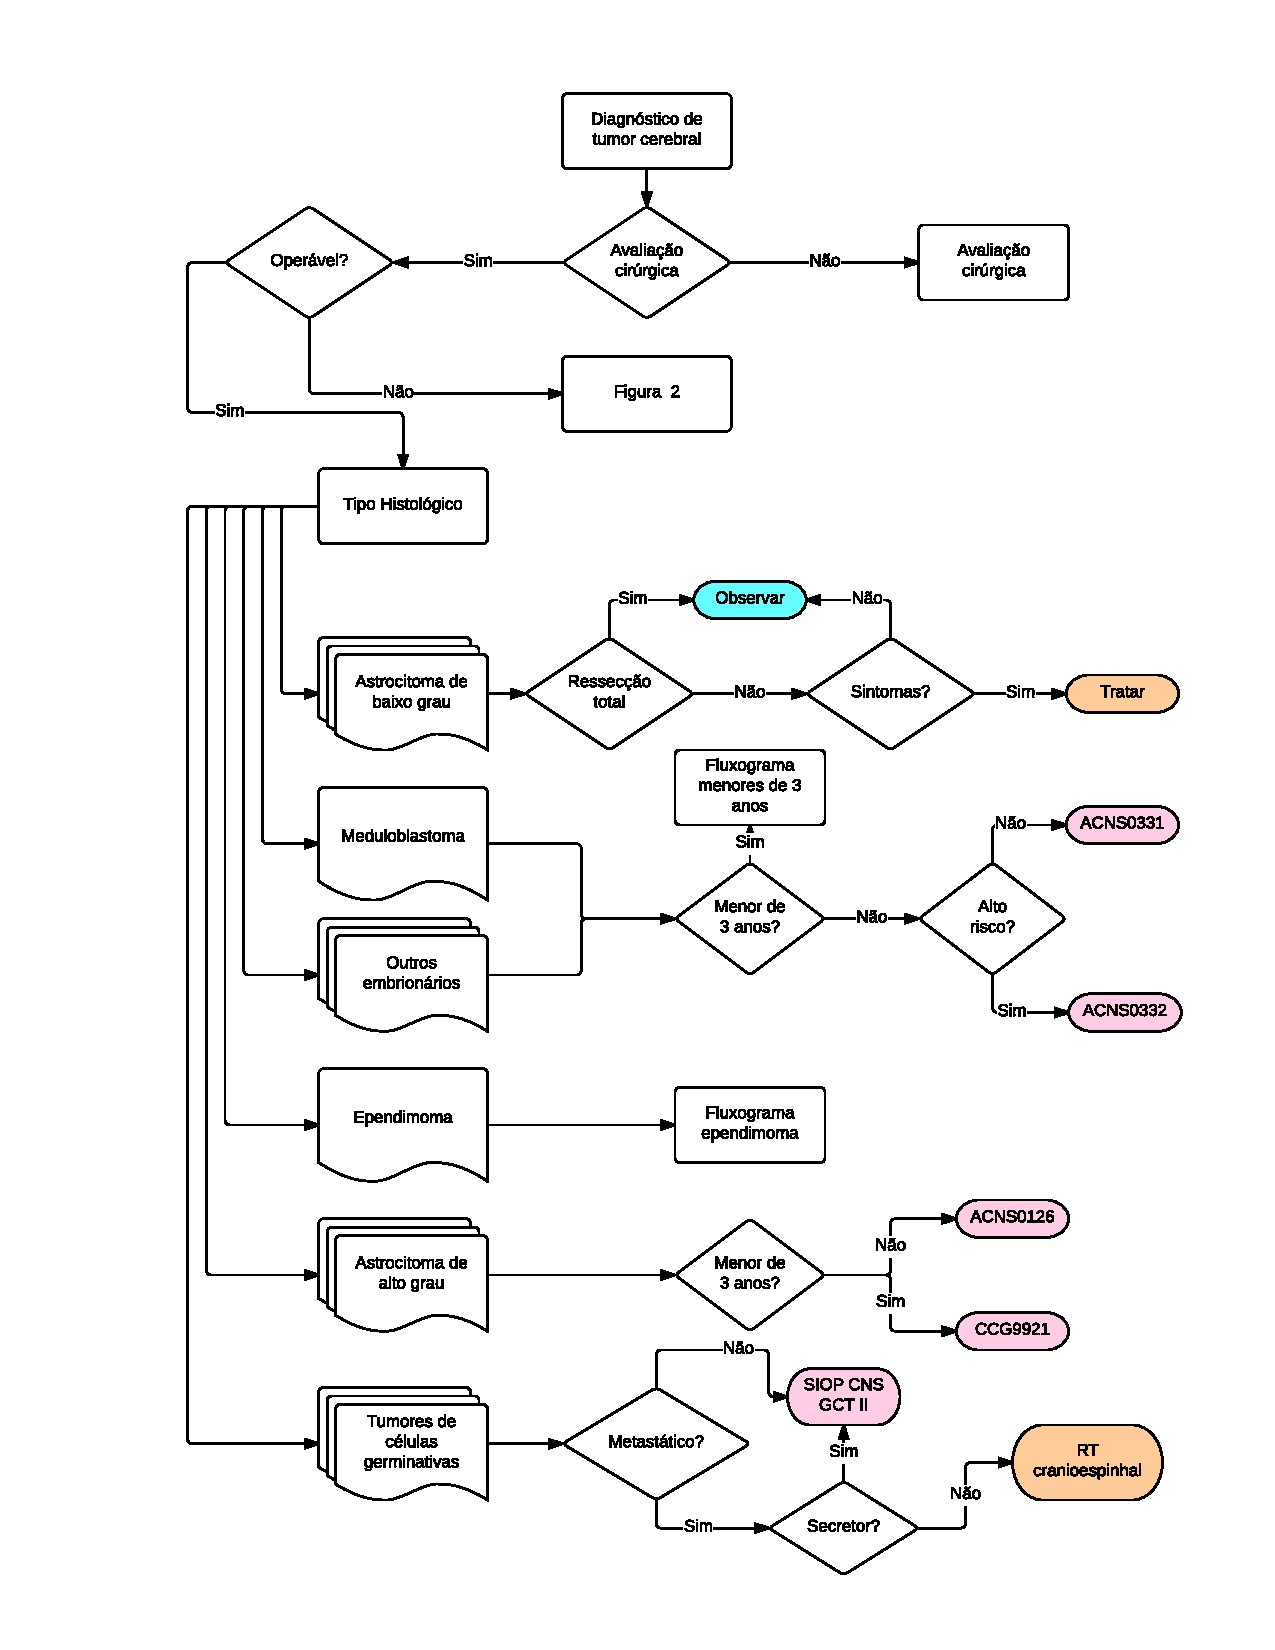
\includegraphics[scale=0.9,trim = 30mm 10mm 8mm 15mm,clip]{fig/fig1.pdf}
\caption{Tratamento de crianças com tumores cerebrais, com histologia}
%\label{Rotulo}
\end{figure}
\begin{figure}[!htb]
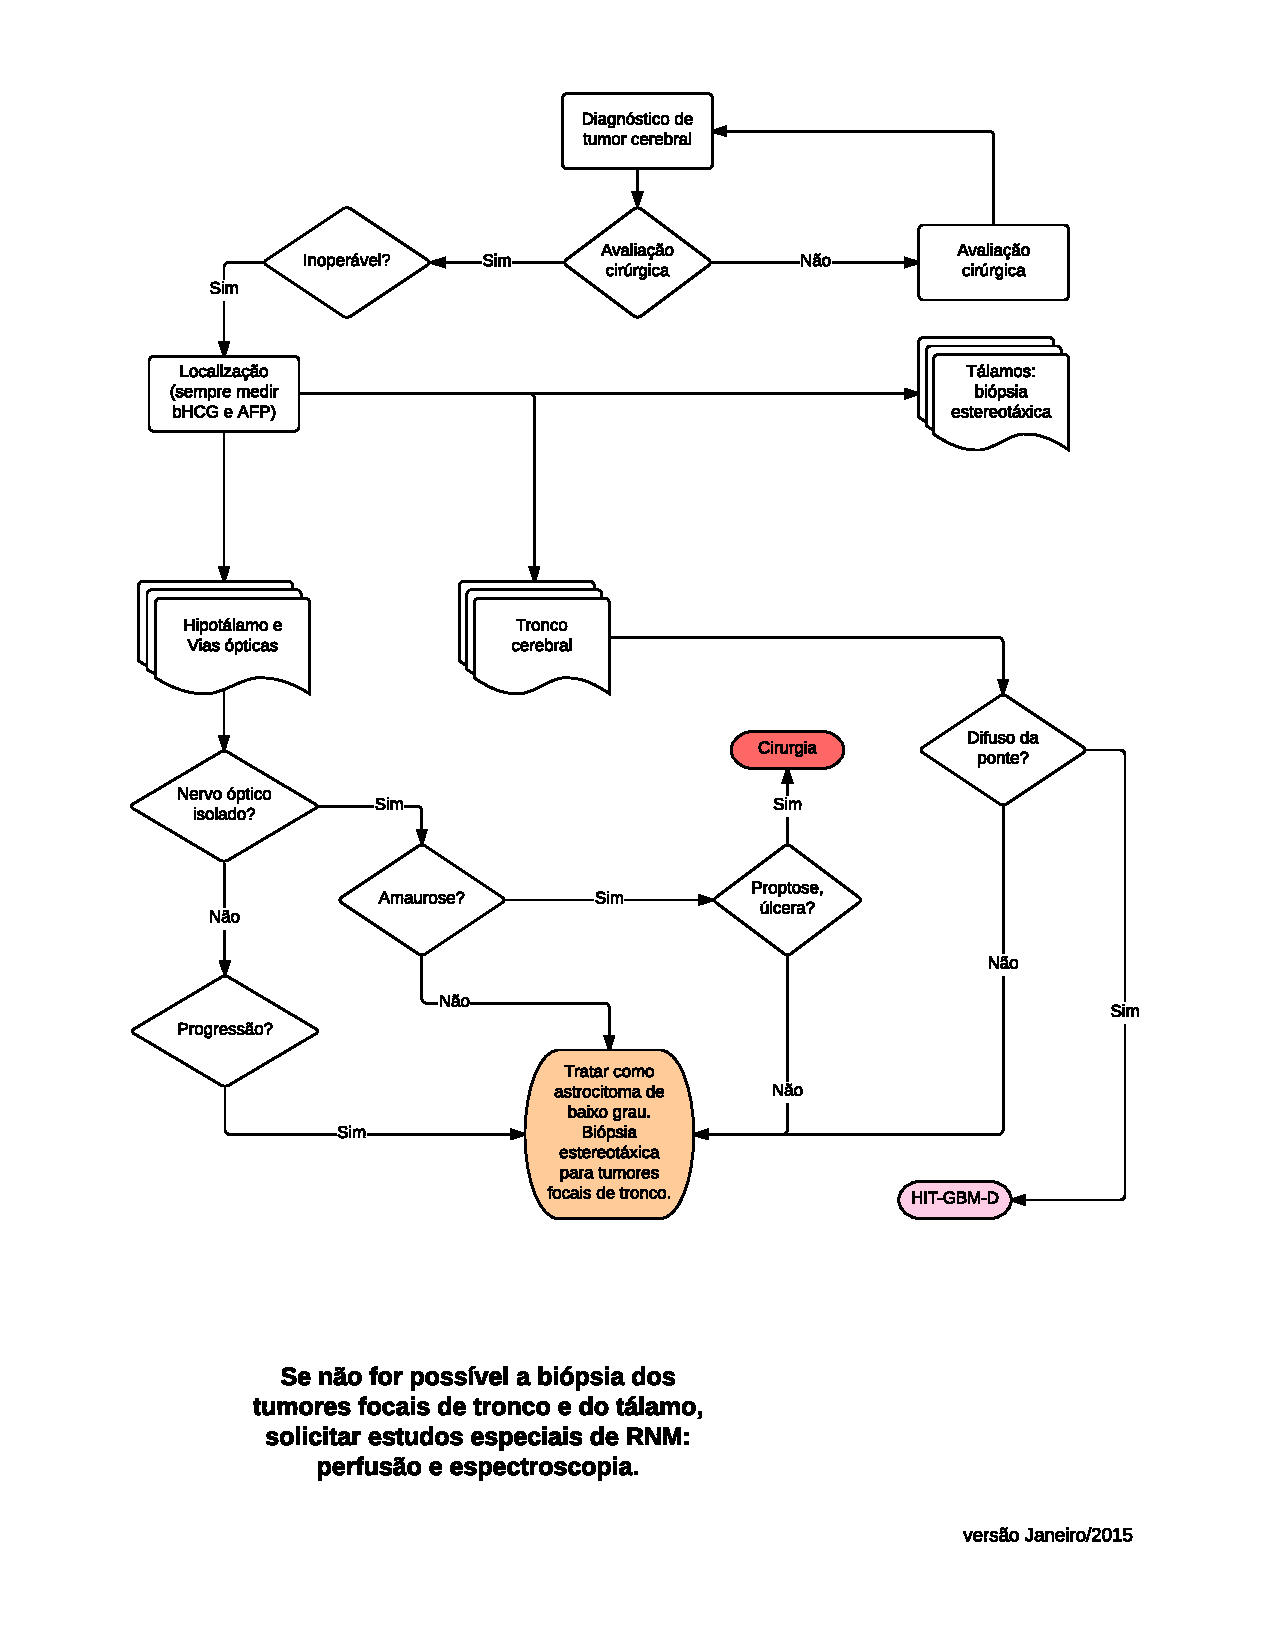
\includegraphics[scale=0.86,trim = 20mm 50mm 10mm 13mm,clip]{fig/fig2.pdf}
\caption{Tratamento de crianças com tumores cerebrais, sem histologia}
%\label{Rotulo}
\end{figure}
\end{center}

Os tumores cerebrais são um grupo heterogêneo de doenças neoplásicas de comportamento variável, com as características comuns de relativa raridade, elevada morbidade e elevada mortalidade. Dentre as neoplasias infantis, no entanto, constituem (como um grupo) o primeiro tumor sólido e a segunda neoplasia maligna mais frequente nas crianças, atrás apenas das leucemias, perfazendo em torno de \(20\%\) das neoplasias pediátricas. A sua incidência varia de acordo com a região do mundo. Nos EUA, a incidência anual ajustada para a idade de tumores cerebrais malignos primários na população de \(0-15\) anos foi de \(3,4\) por \(10^5\) pessoas-ano entre \(2004-2008\) \cite{Ostrom01102014}. Já na Europa, entre \(1988-1997\), a incidência reportada foi de \(2,99\) por \(10^5\) \cite{Peris-Bonet}. Esta incidência é mais alta do que a usualmente reportada na Ásia, onde relatos indicam entre \(1,8-2,2\) casos por \(10^5\) \cite{CNCR21430}. No Brasil, o primeiro relato do Registro de Câncer de Base Populacional indicou uma incidência de \(0,9\) a \(3,2\) por \(10^5\), semelhante à estatística do mundo desenvolvido ocidental \cite{IJC24799}. Fortaleza teve uma das menores incidências relatadas, \(1,3\) casos por \(10^5\), o que pode indicar subdiagnóstico. Hoje em dia, no entanto, já não é apropriado falar em “tumores cerebrais” infantis, sem separar as diversas entidades patológicas entre si, as quais têm incidência, tratamento e prognóstico muito díspares.

Os tumores cerebrais mais frequentes em crianças são os astrocitomas pilocíticos, tumores de comportamento incerto, ora classificados como benignos, ora como malignos. Eles representam em torno de 1\(8\%\) dos tumores cerebrais infantis. Em seguida, vem os tumores embrionários, a maior parte dos quais meduloblastomas, os tumores malignos mais comuns da infància, que representam em torno de \(15\%\) dos diagnósticos de tumor cerebral em crianças \cite{Ostrom01102014}. Astrocitomas pilocíticos são tumores indolentes, de crescimento lento, tratados principalmente pela ressecção cirúrgica, a qual é curativa na maioria dos casos, com pouca probabilidade de disseminação e virtualmente ausência de transformação maligna \cite{gan}. Já os meduloblastomas são tumores indiferenciados, com elevado índice mitótico, com acentuada propensão à disseminação e recidiva, necessitando de terapia adjuvante com radioquimioterapia após ressecção cirúrgica \cite{partap}. Estes dois tipos tumorais, que juntos correspondem a mais de \(30\%\) dos casos de tumores cerebrais em crianças, têm hoje um excelente prognóstico quando comparado ao passado. Outros tipos tumorais menos frequentes, todavia, têm resultados menos brilhantes com o tratamento atualmente disponível. Tumores de tronco cerebral, normalmente não biopsiados na sua maioria, constituem cerca de \(10\%\) dos tumores cerebrais infantis, e têm um prognóstico extremamente reservado, com apenas um subgrupo pequeno de pacientes com tumores neste sítio alcançando sobrevida prolongada.

O tratamento de tumores cerebrais em crianças e adolescentes evoluiu significantemente nas últimas décadas. Dos anos 80 até hoje, o conhecimento sobre o papel das várias modalidades de terapia (cirurgia, radioterapia e quimioterapia) ficou mais claro e programas terapêuticos específicos para cada tipo de doença puderam ser desenvolvidos. Hoje em dia, a maioria das crianças com um diagnóstico de tumor cerebral conseguirá ser adequadamente tratada e alcançará sobrevida prolongada. O manejo dos efeitos colaterais a longo prazo da terapia e das sequelas da doença são as principais preocupações na neuro-oncologia pediátrica moderna \cite{merchant}. No Brasil, estudos de sobrevida de pacientes pediátricos com tumores cerebrais são raros. Nosso grupo publicou recentemente uma análise de sobrevida de \(103\) pacientes pediátricos diagnosticados com tumores cerebrais entre 2000 e 2006 num único centro hospitalar, mostrando resultados que se assemelham aqueles dos registros populacionais dos EUA e Europa para as principais patologias \cite{araujo}.

Os protocolos listados foram avaliados e qualificados segundo a nova classificação de níveis de evidência da OCEBM \cite{ocebm}. A partir desta classificação, foram selecionados os tratamentos com maior qualidade de evidência, os quais podem ser recomendados rotineiramente. Lacunas no conhecimento atual foram listadas (não exaustivamente). De acordo com a classificação 2011 da OCEBM, os ensaios controlados e randomizados são considerados evidência de nível 2, enquanto os estudos não controlados e séries de casos (equivalentes) são considerados evidência de nível 4 (tratamento). Nenhum trabalho com nível 3 de evidência (controlados, porém não randomizados) foi encontrado. Alguns ensaios foram desenhados para obter informações sobre história natural da doença. Grandes coortes para estudo de prognóstico (\textit{inception cohort}) são consideradas nível 2 de evidência, enquanto coortes de qualidade menor ou grupos controle de ensaios randomizados são nível 3.

\section{Por quê criar um compêndio de protocolos de quimioterapia?}
O Hospital Infantil Albert Sabin (HIAS) é uma instituição hospitalar da administração direta da saúde da Secretaria de Saúde do Estado do Ceará, habilitado como unidade de assistência de alta complexidade em neurologia/neurocirurgia, UNACON exclusiva de oncologia pediátrica, UTI pediátrica nível II e hospital de ensino, nível de atenção de alta complexidade, atendendo pelo SUS \cite{cnes}. O Centro Pediátrico do Câncer é o anexo do HIAS onde o tratamento oncológico clínico é realizado, contando ainda com equipe multiprofissional de atenção às crianças com câncer. Tem \(22\) leitos de internação em enfermaria (\(2\) isolamentos), \(06\) leitos de UTIP, e \(05\) consultórios para atendimento ambulatorial. O ambulatório e a enfermaria contam com material para atendimento às urgências e emergências, incluindo carrinho de emergência completo com drogas e equipamento para reanimação. O CPC conta com plantão médico 24h por dia.

O HIAS-CPC é referência estadual para o tratamento de crianças com tumores cerebrais, servindo uma população de 8,8 milhões de habitantes (um e meio milhão de crianças e jovens até 18 anos) \cite{estat}. A incidência ajustada para a idade de tumores cerebrais pediátricos no Ceará foi estimada em \(1,3\) casos por \(10^5\), entre 1998 e 2002 \cite{inca}. Seu papel é fundamental para o diagnóstico, tratamento e acompanhamento de centenas de crianças com câncer, incluindo tumores cerebrais. O HIAS-CPC recebeu cerca de \(35\) novos pacientes com tumores cerebrais ao ano entre 2007 e 2013 (um total de \(250\)). Isto indica que a esmagadora maioria das crianças com esta doença no estado do Ceará são tratadas no HIAS-CPC. Dessa forma, torna-se imprescindível que a qualidade da atenção à saúde dispensada a estes pequenos pacientes em nosso serviço hospitalar seja continuamente revisada, avaliada e padronizada.

\chapter{O tratamento de tumores cerebrais em crianças}

\section{Tumores neuro-epiteliais de baixo grau}

\subsection{Avaliação crítica de ensaios clínicos}
\begin{figure}[!htb]
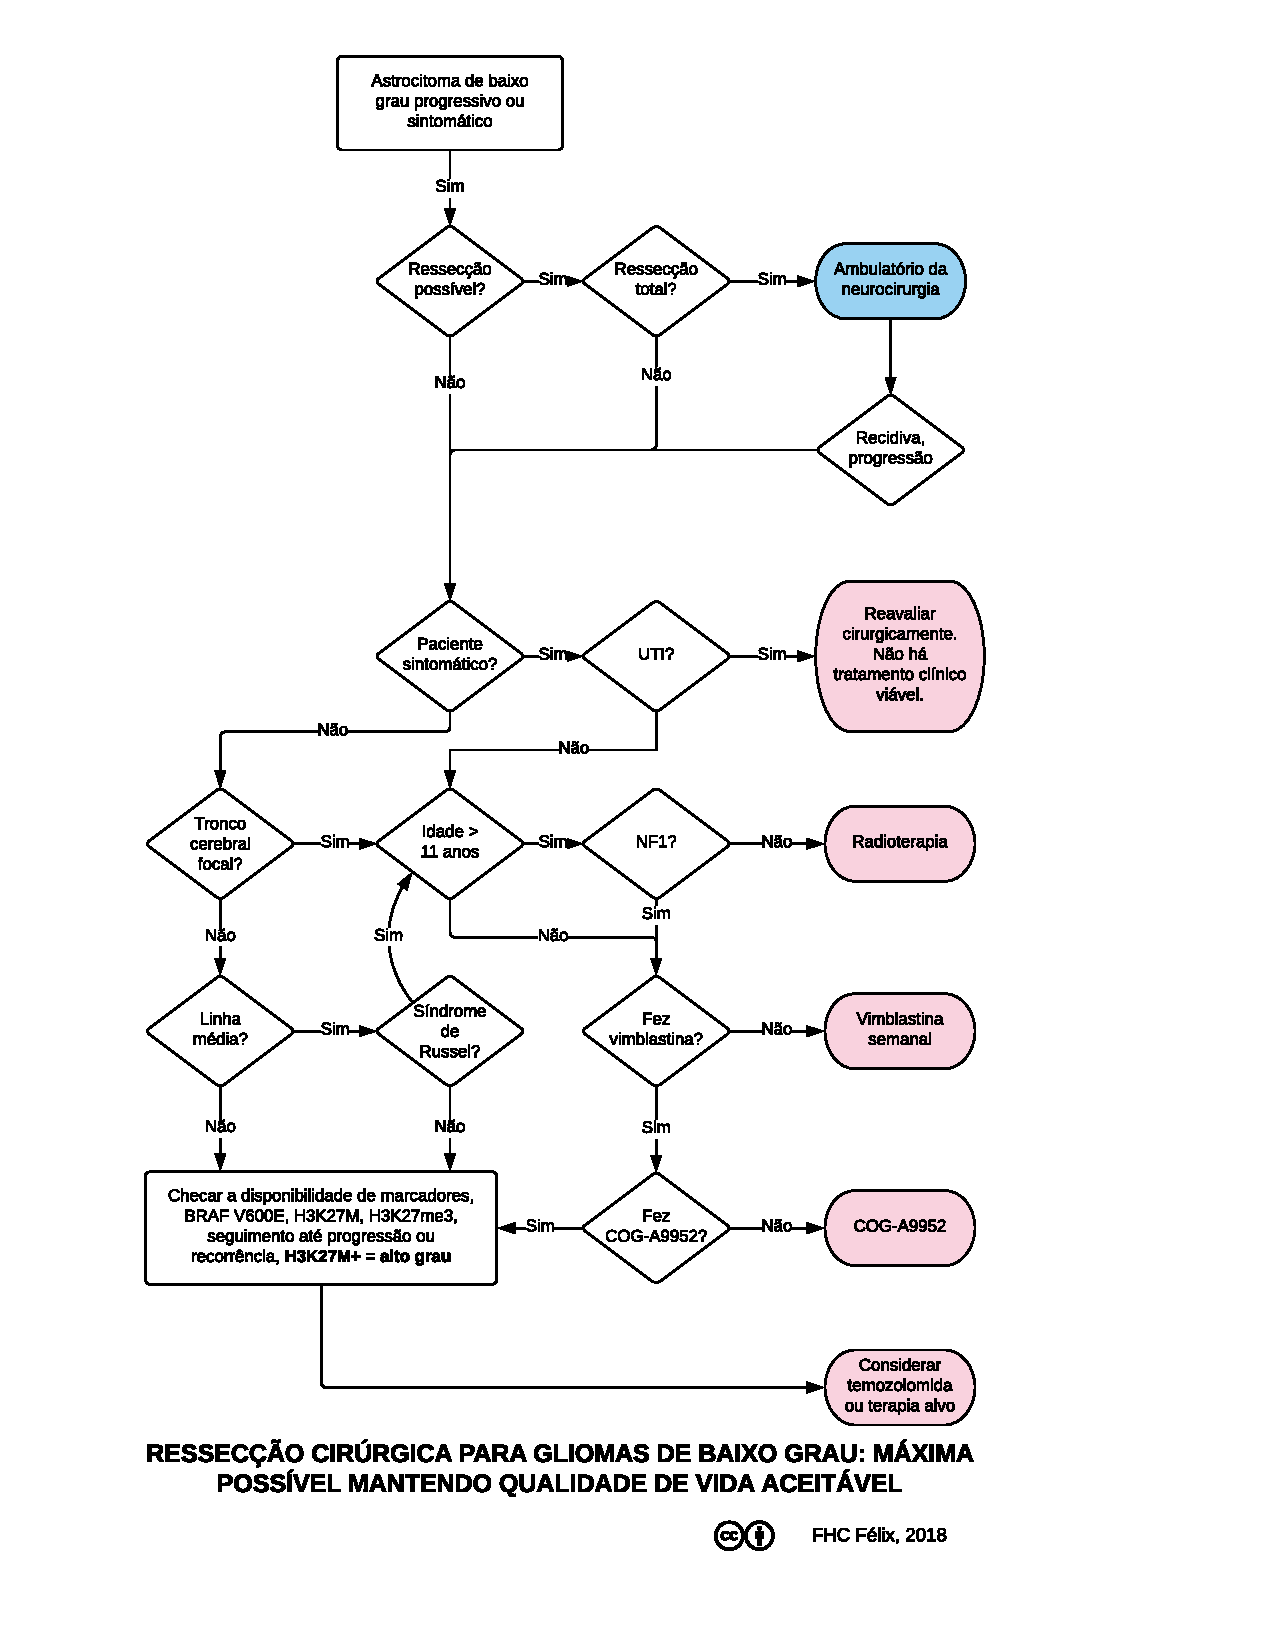
\includegraphics[scale=0.87,trim = 18mm 30mm 15mm 12mm,clip]{fig/fig3.pdf}
\caption{Tratamento de crianças com gliomas e outros tumores neuroepiteliais de baixo grau.}
%\label{Rotulo}
\end{figure}

Esse grupo inclui os astrocitomas, oligodendrogliomas, gangliogliomas e tumores neurogliais mistos ou variantes (grupos IIIa, b e d da ICCC3) \cite{CNCR20910}. A denominação de baixo grau refere-se à classificação da OMS para tumores do sistema nervoso central, a qual divide as neoplasias em 4 grupos, baseada em critérios histológicos. A classificação da OMS para tumores do sistema nervoso central constitui uma “escala de malignidade”, mais do que um esquema de estadiamento convencional \cite{louis}. Os tumores classificados como Grau I ou II são coletivamente denominados tumores de baixo grau de malignidade, enquanto aqueles classificados como Grau III ou IV são designados tumores de alto grau de malignidade. Os tumores de baixo grau são comumente tratados apenas cirurgicamente, com elevados índices de cura e sobrevida prolongada. Tumores astrocíticos e oligodendrogliais de baixo grau têm bom prognóstico associado à ressecção cirúrgica como única terapia. Todavia, a possibilidade de ressecção cirúrgica completa varia muito de acordo com o sítio tumoral \cite{wisof}.

Gliomas cerebelares são passíveis de ressecção completa em \(60-70\%\) dos casos, a maioria são astrocitomas pilocíticos (grau I) e seu comportamento é praticamente benigno \cite{gan}. A recidiva após ressecção e a progressão para tumores de maior grau de malignidade são muito raras. Mesmo tumores incompletamente ressecados mostram uma baixa propensão a progredir. A sobrevida livre de progressão em 5 anos após a cirurgia é de \(84-91\%\). A sobrevida livre de progressão em 5 anos em pacientes com doença residual é de \(54-63\%\) \cite{wisof}. 

Gliomas da via óptica e hipotálamo (e demais tumores diencefálicos ou da linha média) são lesões difusas, infiltrativas, em sua maioria astrocitomas de baixo grau (pilocítico ou difuso), com maior chance de disseminação e metástase no neuro-eixo, com maior incidência em pacientes com neurofibromatose tipo 1. Devido a sua natureza infiltrativa e ao risco de sequelas visuais e neuro-endócrinas, a ressecção cirúrgica não é realizada na maioria dos casos e a biópsia somente está indicada nos casos de imagem atípica. A maioria dos pacientes é tratada com base apenas em imagens sugestivas. Apesar de sua histologia, têm um prognóstico mais reservado do que os pacientes com lesões cerebelares \cite{gan}. A sobrevida livre de progressão em 5 anos é de \(47\%\) \cite{wisof}. 

Oligodendrogliomas, tumores mistos e variantes de tumores astrocíticos são raros em crianças (\(1\%\) ou menos de todos os tumores cerebrais). São tumores da substância branca supratentorial, infiltrativos, e o controle cirúrgico é curativo na maioria. Terapia adjuvante não está bem definida para estes tumores \cite{gan}. A sobrevida livre de progressão em 5 anos é de \(67\%\) \cite{wisof}.

O papel da cirurgia no controle dos gliomas de baixo grau está bem estabelecido. O estudo prospectivo multi-institucional do Children’s Oncology Group (COG) CCG9891 avaliou uma coorte de \(518\) pacientes diagnosticados com tumores de origem glial, tratados inicialmente com ressecção cirúrgica. Ocorreu revisão central da histologia de todos os casos incluídos. Do total, \(64\%\) dos pacientes não tinha evidência de doença residual após a cirurgia, \(20\%\) tinha doença residual limitada (\(< 1,5 cm^3\)) e \(16\%\) tinha doença residual significante (\(> 1,5 cm^3\)). A maioria dos pacientes (\(76\%\)) tinha astrocitoma pilocítico, \(6\%\) astrocitoma difuso, \(8\%\) ganglioglioma e \(10\%\) oligodendroglioma, tumores mistos ou variantes. A maioria dos pacientes (\(73\%\)) tinha 5 anos ou mais. A maioria (\(57\%\)) tinha tumores cerebelares, \(24\%\) de hemisférios cerebrais, \(14\%\) da linha média e \(4\%\) das vias ópticas ou hipotálamo. 

A sobrevida livre de progressão (SLP) em 5 anos de toda a coorte foi de \(80\%\), sendo \(84 \:a\: 91\%\) para tumores cerebelares, \(78\%\) para hemisférios cerebrais, \(65\%\) para a linha média e \(47\%\) para vias ópticas ou hipotálamo (\(p<0,001\)) (nível 2). A SLP em 5 anos foi de \(83\%\) para astrocitomas pilocíticos, \(88\%\) para gangliogliomas, \(66\%\) para astrocitomas difusos e \(67\%\) para outros tumores (\(p=0,64\)) (nível 2). Finalmente, a ressecção cirúrgica completa foi o fator isolado de maior impacto na progressão nesta coorte, \(94\%\) dos pacientes com ressecção completa estavam livres de progressão após 5 anos, enquanto \(59\%\) dos pacientes com doença residual limitada e \(53\%\) dos pacientes com doença residual significante alcançaram sobrevida livre de progressão prolongada (\(p<0,01\)) (nível 2). 

A conclusão é de que a ressecção completa deve ser tentada sempre que possível (ou seja, desde que não acarrete comprometimento funcional) para os pacientes pediátricos com gliomas de baixo grau (nível 4). Além disso, o fato de que mais de \(50\%\) dos pacientes com doença residual não progrediram em 5 anos indica que as intervenções terapêuticas adjuvantes devem ser postergadas até que ocorra progressão objetiva da doença. No entanto, apesar de sua histologia aparentemente benigna, \(44\%\) dos pacientes progrediram mesmo com doença residual muito limitada, o que indica a necessidade de monitorização dos pacientes com ressecção incompleta, independente da quantidade de tumor residual (nível 2) \cite{wisof}.

Fica evidente que um número significativo de pacientes pediátricos com gliomas de baixo grau sofre recidiva após controle cirúrgico ou não pode ter seu tumor ressecado. Nestes casos, indica-se terapia adjuvante com a intenção de evitar a progressão da doença. Vários estudos exploraram a contribuição da radioterapia e quimioterapia no tratamento de gliomas de baixo grau progressivos. 

Um ensaio fase II não controlado estudou 78 crianças com gliomas de baixo grau tratadas com radioterapia conformacional. Os pacientes tinham astrocitoma pilocítico (\(n=50\)), tumores de via óptica ou hipotálamo sem biópsia (\(n=13\)), astrocitoma difuso (\(n=4\)), ganglioglioma (\(n=3\)) e oligodendroglioma, tumores mistos ou variantes (\(n=8\)). A maioria dos tumores localizava-se no diencéfalo (\(47\)), \(17\) no cerebelo e \(3\) nos hemisférios cerebrais. Treze pacientes tinham NF-1, \(25\) receberam QT previamente e \(65\) sofreram cirurgia (biópsia ou ressecção incompleta). O tratamento foi indicado nos pacientes sintomáticos na avaliação inicial ou com evidência radiológica de progressão ou, ainda, com uma lesão residual numa área de risco para progressão. Dentre os pacientes cujo tratamento primário foi radioterapia, mais da metade iniciou o tratamento em menos de 90 dias após o diagnóstico. 

A SLP em 5 anos do grupo foi de \(87\%\). Treze pacientes apresentaram progressão com uma mediana de tempo de \(83\) meses. Quatro pacientes apresentaram falha terapêutica, desenvolvendo doença metastática. Não ocorreu diferença digna de nota entre os tipos histológicos (nível 2). Nenhum dos pacientes com NF-1 teve progressão ou malignização. Um paciente da série desenvolveu um glioma de alto grau na região do campo de irradiação, \(78\) meses após o tratamento. A incidência cumulativa de vasculopatia na série foi de cerca de \(5\%\) em 7 anos e o principal fator de risco para esta complicação foi a idade menor que 5 anos (nível 2) \cite{Merchant01082009}. Em relação aos efeitos cognitivos, um declínio de \(10\) pontos de QI foi estimado para crianças com 5 anos de idade ao tratamento, 5 anos após a radioterapia. O risco cumulativo de desenvolver insuficiência tireoidiana foi de \(64\%\) e de deficiência de GH foi de \(49\%\), em 10 anos. A incidência cumulativa de déficit auditivo foi de cerca de \(6\%\) em 10 anos. A presença de NF-1 foi um fator de risco para vasculopatia e déficit cognitivo (nível 2) \cite{Merchant01082009.2}. 

Em conclusão, esta série mostrou inequivocamente que a radioterapia pode controlar adequadamente os gliomas de baixo grau pediátricos não controlados cirurgicamente, com uma elevada proporção de pacientes tendo sobrevida prolongada sem progressão (nível 4). No entanto, isso ocorre às custas de frequentes efeitos colaterais, provavelmente permanentes. A radioterapia para gliomas de baixo grau deve ser evitada em pacientes com menos de 5 anos, devido ao risco de vasculopatia (nível 2). Apesar do risco cumulativo de déficit auditivo ser baixo e do fato do declínio cognitivo ser menor com o avançar da idade, adiar a radioterapia o quanto for possível parece razoável.

Com o intuito de atrasar o início da radioterapia, vários estudos foram realizados com diferentes esquemas de quimioterapia em crianças com gliomas de baixo grau recorrentes ou progressivos. As combinações mais utilizadas foram: carboplatina e vincristina \cite{packer,gnekow}; procarbazina, tioguanina, lomustina e vincristina (TPCV) \cite{prados}; cisplatina e etoposido \cite{mass}.

Packer \textit{et al} trataram \(78\) pacientes até 15 anos (idade média 3 anos, variando de 3 meses a 16 anos) com gliomas de baixo grau confirmados por histologia ou imagem típica, progressivos, reportando \(56\%\) de resposta radiológica objetiva e \(68 \pm 7\%\) de SLP em 3 anos (nível 4). A maioria dos pacientes (\(n=32\)) tinha astrocitoma fibrilar (difuso), \(17\) tinham astrocitoma pilocítico e \(26\) não tinham histologia. A maioria dos pacientes tinha tumores diencefálicos (\(n=58\)), \(12\) tinham no tronco e \(6\) em outros locais. Somente pacientes que sofreram ressecção de \(50\%\) ou menos das lesões foram admitidos. Não ocorreu revisão central de histologia ou imagens. Este ensaio clínico não avaliou se o esquema conseguia adiar o início da radioterapia, principal motivo do tratamento, devido ao curto tempo de seguimento \cite{packer}. 

A carboplatina fora testada pelo Pediatric Oncology Group (POG), em comparação com a iproplatina, num ensaio fase II, randomizado. Um grupo de pacientes pediátricos com tumores cerebrais histologicamente verificados, recorrentes ou progressivos, foi avaliado. O subgrupo de pacientes com astrocitoma de baixo grau (\(12\) pacientes, agregando pacientes de um ensaio não randomizado prévio do POG) não mostrou resposta radiológica objetiva, mas a maioria dos pacientes apresentou estabilização prolongada da doença com a carboplatina, o que motivou os pesquisadores a testá-la num grupo maior \cite{fried}. 

Prados \textit{et al}  trataram \(42\) crianças até 18 anos com gliomas de baixo grau histologicamente confirmados (exceto tumores de diencéfalo em pacientes com NF-1 ou de vias ópticas), com doença progressiva, utilizando a combinação TPCV. A SLP foi de \(45\%\) em 3 anos, com mediana de \(2,5\) anos para progressão (nível 4). A maioria dos pacientes tinha astrocitoma pilocítico (\(n=23\)), \(11\) tinham astrocitoma (sem outra especificação), \(6\) não tinham histologia e \(2\) tinham oligodendroglioma ou ganglioglioma. A maioria dos pacientes tinham tumores hipotalâmicos ou quiasmáticos (\(n=33\)), \(4\) talâmicos e \(5\) em outras localizações. A maioria dos pacientes sofreu ressecção parcial ou subtotal. Este esquema foi derivado de experimentos pré-clínicos que mostraram que a combinação das drogas utilizadas tinha efeitos sinérgicos nas células neoplásicas \cite{prados}. 

O ensaio não randomizado HIT-LGG 1996, do grupo de pediatria oncológica dos países de língua alemã (GPOH) utilizou um esquema de carboplatina e vincristina diferente daquele do COG. Um relato do subgrupo com gliomas hipotalâmico-quiasmáticos que recebeu quimioterapia (\(n=123\)) mostrou SLP de \(61\%\) em 5 anos \cite{gnekow} (nível 4). Os resultados completos do ensaio foram publicados em 2012 \cite{gnekow2}. Um total de \(1031\) pacientes foram recrutados, em um braço sem intervenção pós-cirurgia (ressecção total ou parcial, \(n = 668\)), e outro braço (não cirúrgico ou ressecção parcial) estratificado de acordo com a idade para receber vincristina-carboplatina (\(n = 216\)) ou radioterapia/braquiterapia convencional (\(n = 147\)). A idade média foi 6,9 anos, \(40\%\) dos pacientes tinha tumores de linha média e \(68\%\) tinha astrocitoma pilocítico. 

A sobrevida livre de eventos (SLE) em 5 e 10 anos relatada foi de \(47\%\) e \(44\%\) para o grupo tratado com quimioterapia e \(65\%\) e \(62\%\) para o grupo tratado com radioterapia. Entre os fatores afetando adversamente o prognóstico foram observados: ressecção cirúrgica imcompleta, idade < 1 ano ou > 11 anos, sítio tumoral de linha média (nível 4 para tratamento e nível 2 para prognóstico). Sessenta e um dos pacientes tratados com quimioterapia receberam radioterapia 0,3-8,7 anos após o primeiro tratamento. O ensaio não comparou o braço tratado apenas com cirurgia com aquele tratado com terapia adjuvante \cite{gnekow2}. 

Com o intuito de tentar melhorar estes resultados, a SIOP e o GPOH iniciaram conjuntamente o ensaio SIOP-LGG 2004, o qual terminou de cadastrar pacientes em 2012. Este ensaio randomizado compara carboplatina e vincristina com carboplatina, vincristina e etoposide \cite{gnekow3}. 

Em 2002, um grupo italiano relatou um grupo de 34 crianças com gliomas de baixo grau não ressecáveis, a maior parte hipotalâmico-quiasmáticos (\(n=29\)), tratadas com cisplatina e etoposide. Eles mostraram uma SLP de \(78\%\) em 3 anos, com \(11\) pacientes obtendo remissão parcial e 1 completa (nível 4). No entanto, uma quantidade significativa de pacientes apresentou toxicidade auditiva, um efeito colateral conhecido da cisplatina \cite{mass}.

Apesar da aparente superioridade da combinação carboplatina e vincristina, os ensaios tinham grandes diferenças entre si quanto aos diagnósticos histológicos e topográficos dos pacientes, além de diferenças na terapia prévia. Para definir qual o melhor dentre os dois esquemas, um ensaio fase III randomizado foi levado a cabo pelo COG e seus resultados publicados recentemente \cite{Ater20072012}. O estudo avaliou \(274\) pacientes com 10 anos ou menos, com gliomas de baixo grau e com doença residual (mais de \(5\%\) da lesão inicial ou \(1,5 cm^2\)) ou progressiva. Ocorreu revisão central das imagens e da patologia. Pacientes com tumores hipotalâmico-quiasmáticos foram incluídos com base nas imagens. 

A SLP em 5 anos foi de \(45\%\) para todo o grupo, sendo de \(39\%\) para o esquema carboplatina-vincristina e \(52\%\) para o esquema TPCV. Esta diferença não foi significante num teste de log-rank, mas mostrou-se significante num modelo de sobrevida com fração de cura (cure rate model), onde parte desta diferença deveu-se a pacientes com sobrevida prolongada (\(p<0,05\)) (nível 2). O ensaio encontrou dois preditores independentes da SLP: idade (menor risco entre 1 e 5 anos) e doença residual (menor risco se \(<3 cm^2\)) (nível 2).

Em 2016, o grupo de neuro-oncologia pediátrica do Canadá publicou os resultados de um ensaio fase II que testou a monoterapia com vimblastina semanal para pacientes pediátricos com tumores neuroepiteliais de baixo grau progressivos \cite{lassaletta}. Cinquenta e quatro pacientes (idade média 8 anos, variando de 0,7 a 17), a maioria (\(~ 50\%\)) com tumores da linha média anterior (quiasma óptico e hipotálamo) e astrocitoma pilocítico foram tratados com vimblastina semanal. Quarenta e sete pacientes (\(87\%\)) obtiveram pelo menos estabilização da doença. A SLP em 5 anos foi de \(53\%\) (intervalo ce confiança 95\% 41-68). Pacientes com NF-1 (17 pacientes) mostraram melhor sobrevida livre de progressão, \(85\% (IC95 68-100)\), do que pacientes sem NF-1 (\(42\%, IC95 29-60, p = 0.01\)). Não ocorreu diferença em relação à presença de alterações genéticas de BRAF (nível 4).

O resultado destes ensaios deve ser encarado com senso crítico. Apesar de todos os regimes terapêuticos aparentemente terem conseguido adiar a progressão nos pacientes estudados, nenhum estudo comparou os resultados com um grupo controle randomizado ou não. O fato de que o subgrupo com doença residual do ensaio CCG9891 também ter apresentado SLP equivalente indica que se deve ter cautela na indicação de tratamentos adjuvantes. Uma comparação entre os regimes e com um grupo controle não tratado parece estar justificada. Além disso, uma melhor caracterização dos subgrupos onde o tratamento farmacológico tem utilidade é necessário.

\subsection{O panorama molecular dos gliomas de baixo grau}

Até 2016, a classificação dos tumores do sistema nervoso central agregava o conhecimento anátomo-patológico e clínico acumulado em 130 anos de neuropatologia desde o trabalho pioneiro de Santiago de Ramón y Cajal \cite{pinero2014santiago}. Neste ano, a Organização Mundial da Saúde (OMS) publicou a revisão de sua quarta edição da Classificação dos Tumores do Sistema Nervoso Central \cite{Louis2016}. Pela primeira vez, a classificação incluiu dados moleculares oriundos de estudos genômicos empreendidos nos últimos 15 anos, desde a conclusão do Projeto Genoma Humano. Dessa forma, o conhecimento sobre as alterações moleculares mais frequentes em gliomas de baixo grau foram agregadas à avaliação clínico-patológica destes tumores, com valor prognóstico já demonstrado. Este novo conhecimento ainda não originou mudanças na prática clínica, tanto em termos de estratificação de grupos de risco, quanto em relação à terapia. No entanto, isso será somente questão de tempo. Até o momento, acumulam-se relatos de casos publicados mostrando resposta de pacientes com gliomas de baixo grau com alterações moleculares bem definidas à terapia alvo direcionada a estas alterações moleculares. Desa forma, é provável que os ensaios clínicos do futuro passem a estratificar os pacientes de acordo com a classificação molecular e que eles sejam tratados de acordo com medicações sem citotoxidade geral, como os inibidores de tirosina quinase \cite{now209}.

A principal doença desse grupo a ter seu panorama molecular definido também é a mais comum em crianças e adolescentes: astrocitoma piloćitico. Em 2008, foi descrita uma duplicação gênica em tandem no locus 7q34, a qual criava um gene quimérico pela fusão KIAA1549:BRAF em 29 de 44 casos de pacientes com astrocitoma pilocítico. O produto gênico é uma proteína com atividade proteína quinase constitutiva capaz de transformar células gliais \cite{Jones8673}. Essa foi a primeira mutação deste tipo (rearranjo gênico) afetando a via RAS/RAF documentada em um tumor esporádico. Uma avaliação de 64 casos pediátricos de astrocitoma pilocítico mostrou a presença da mutação pontual V600E do gene BRAF em 6 pacientes e uma mutação B-Raf\textsuperscript{insT}(inserção causando duplicação da treonina 599) em mais 2 pacientes\cite{IJC25893}. Somando-se o número de pacientes com astrocitoma pilocítico que comumente têm NF-1 ou fusões mais raras com RAF1, pode-se concluir que cerca de 80-90\% dos pacientes com esse tumor apresentam uma mutação da via MAPK/ERK (\textit{mitogen-activated protein kinase/extracellular signal-regulated kinase}, caracterizando esta via de sinalização celular como crítica para a gênese deste tumor \cite{Jones2012}. Aparentemente, as diversas mutações são mutuamente excludentes no astrocitoma pilocítico, ou seja os pacientes negativos para a fusão KIAA1549:BRAF ou têm o gene não mutado ou BRAF\textsuperscript{V600E} (ou ainda uma outra mutação mais rara de BRAF). O perfil molecular também influencia a localização dos tumores: NF1 e mutações pontuais de BRAF são mais comuns em tumores de linha média, já as fusões envolvendo BRAF ou RAF1 são mais encontradas no cerebelo \cite{Jones2012}. 

A fusão KIAA1549:BRAF nunca foi demonstrada de forma incontroversa em outros gliomas que não o astrocitoma pilocítico, o que parece indicar que é uma alteração genética praticamente exclusiva deste tumor. Isso dá valor diagnóstico importante em casos de dúvida. De fato, a tendência é considerar os raros casos de "outros gliomas" positivos para esta fusão como sendo, na verdade, variantes histológicas incomuns do astrocitoma pilocítico \cite{Jones2012}. Em contraste, a mutação BRAF\textsuperscript{V600E} não é exclusiva de um tipo tumoral apenas, ocorrendo em mairo frequência em casos de melanoma, carcinoma de cólon e de tireóide. Além de uma pequena porcentagem de astrocitomas pilocíticos, essa mutação é encontrada em vários gliomas de baixo grau menos comuns. Uma análise de 1320 casos de tumores primários do sistema nervoso central mostrou positividade de BRAF\textsuperscript{V600E} em 42 de 64 (66\%) de xantoastrocitomas pleomórficos, 15 de 23 (65\%) de xantoastrocitomas pleomórficos anaplásicos, 14 de 77 (18\%) de gangliogliomas e 9 de 97 (9\%) de astrocitomas pilocíticos. Neste último tumor, um terço foram detectados em tumores diencefálicos \cite{Schindler2011}. Dessa forma, a via MAPK/ERK de sinalização celular surge como a principal envolvida na gênese dos gliomas de baixo grau de uma forma em geral, especialmente astrocitoma pilocítico, ganglioglioma e xantoastrocitoma pleomórfico.

Outras alterações genéticas têm sido descritas neste grupo de tumores, sendo que uma das mais recentes é a presença de mutações dos genes MYB e MYBL1 no glioma angiocêntrico e astrocitoma difuso \cite{Tatevossian2010}. Uma avaliação genômica de 91 tumores neuroepiteliais de baixo grau menos comuns identificou um marcador genético único em 84\% dos casos. Uma fusão MYB-QKI foi identificada em 87\% dos gliomas angiocêntricos e rearranjos envolvendo MYB/MYBL1 foram encontradas em 41\% dos astrocitomas difusos. Esses dados comprovam alterações destes genes como as mais importantes nestes dois tipos de tumores gliais \cite{Qaddoumi2016}. Mutações pontuais de FGFR1 são as mais comuns em gliomas de baixo grau depois da mutação BRAF\textsuperscript{V600E} \cite{now209}. Uma alteração genética de FGFR1, incluindo mutações pontuais, duplicações internas do domínio quinase e fusões foram encontradas em 82\% de DNET (\textit{dysembrioplastic neuroepithelial tumors}) e 40\% de tumores oligodendrogliais, na mesma avaliação genômica.

Fica claro pelos dados de pesquisa genômica associada com clínica nos últimos 10-15 anos que as alterações moleculares mais frequentes em tumores neuroepiteliais de baixo grau ocorrem em 3 genes: BRAF, MYB e FGFR1 \cite{now209,Qaddoumi2016}. Outras alterações moleculares descritas parecem girar em torno das vias de sinalização molecular representadas por estes mesmos genes. Isso abre uma nova era de possibilidades para diagnóstico e terapia baseadas em biologia molecular. Os ensaios clínicos do futuro vão rapidamente agregar estes dados para definir subgrupos de prognóstico bem definido e validar o tratamento com terapia-alvo.

\subsection{Questões importantes ainda por responder}

A evidência apresentada até o momento deixa uma série de lacunas em nosso conhecimento sobre o tratamento clínico de tumores neuroepiteliais de baixo grau em crianças e adolescentes. Entre as diversas questões que podemos levantar, algumas podem ser apontadas como mais evidentes:

\begin{enumerate}
\item Pacientes com tumor residual maior que \(1,5 cm^2\) e menor que \(3,0 cm^2\) serão melhor seguidos com conduta expectante? 
\item Para pacientes com mais de 5 anos e mais de \(3,0 cm^2\) de tumor residual, deve-se indicar radioterapia precocemente? 
\item A quimioterapia tem papel restrito aos pacientes menores de 5 anos com progressão documentada e naqueles com gliomas hipotalâmico-quiasmáticos? 
\item Deve-se adaptar a estratégia terapêutica de acordo com o sítio tumoral?
\item A vimblastina semanal deve ser a primeira escolha de tratamento quimioterápico?
\item Qual o melhor tratamento após falha terapêutica múltipla (progressão após dois tratamentos com quimioterapia e/ou radioterapia)?
\end{enumerate}

A ausência de ensaios comparativos entre as abordagens terapêuticas e de ensaios com controles não tratados impede a resposta destas questões com certeza. A realização de ensaios clínicos com desenho e poder estatístico para responder estas questões com a maior certeza possível vai exigir uma inédita colaboração internacional, com a participação ativa de centros de tratamento ao redor do mundo. A partir desse esforço, será possível oferecer o melhor e mais eficiente tratamento a todas as crianças e adolescentes com esta patologia.

\subsection{Conclusões}

A conclusão sobre a terapia dos tumores neuroepiteliais de baixo grau é de que, hoje em dia, temos evidência de relativa boa qualidade documentando a história natural deste grupo de tumores, mas a ausência de adequados estudos controlados e randomizados ainda suscita dúvidas quanto à melhor conduta em cada situação. A partir dos dados que temos até o momento, um esquema racional de tratamento para gliomas de baixo grau pediátricos inclui:

\renewcommand{\labelenumi}{\Alph{enumi}}
\begin{enumerate}
\item - A melhor ressecção cirúrgica possível (mantendo ao máximo a função) (nível 2)
\item - Seguimento de todos os pacientes com doença residual (independente da quantidade) (nível 2)
\item - Aguardar a progressão (ou piora sintomática) para indicar terapia adjuvante (mesmo quando doença residual) (nível 2)
\item - Evitar radioterapia em menores de 5 anos e portadores de NF-1 através do uso de quimioterapia (TPCV um pouco superior a carboplatina-vincristina, vimblastina parece ser equivalente) (nível 4)
\item - Tratar com radioterapia lesões progressivas após cirurgia e/ou quimioterapia, em maiores de 8-10 anos (nível 4)
\end{enumerate}

Infelizmente, mesmo com essa abordagem baseada em evidência, uma quantidade significativa de pacientes terá doença progressiva apesar da melhor terapia, mostrando que o tratamento ótimo dos tumores neuro-epiteliais de baixo grau pediátricos ainda não foi atingido. A incorporação de marcadores moleculares e melhor definição de subgrupos de risco devem ser prioridades na agenda da pesquisa clínica.

\section{Tumores embrionários e pineoblastoma}

Tumores embrionários incluem o meduloblastoma (mais comum deste grupo e o tumor cerebral maligno mais frequente em crianças e adolescentes), tumor teratóide-rabdóide atípico, tumor embrionário formador de rosetas em multicamadas, tumor embrionário sem outra especificação (SOE) e outros tumores mais raros. 

\bibliographystyle{unsrt}
\bibliography{bib}

\chapter{Esquemas de tratamento}

\section{Introdução}
No Centro Pediátrico do Câncer do Hospital Infantil Albert Sabin, utilizamos um total de 16 (dezesseis) protocolos de tratamento farmacológico para tumores cerebrais em crianças e adolescentes, baseados na literatura que foi citada neste manual. Estes protocolos foram adaptados a partir dos racionais dos ensaios clínicos descritos, com modificações pertinentes à realidade e disponibilidade de recursos em nosso serviço hospitalar. Além disso, quaisquer conclusões oriundas dos resultados destes ensaios clínicos, bem como informações de outros trabalhos e de outras fontes, foram usadas para adaptar os esquemas de tratamento à luz da melhor evidência disponível no momento em que este manual foi escrito. Alguns dos ensaios clínicos utilizados como modelo para parametrizar nossos protocolos ainda estão em andamento. Neste caso, apenas a parte não randomizada, não experimental dos esquemas foi adaptada e utilizada, mas não os braços de tratamento experimental ou não comprovado por evidências científicas.

Pacientes com condições patológicas que não têm nenhum tratamento amplamente aceito, ou sobre as quais recaem controvérsias importantes quanto à terapêutica, não poderão ser tratados com os protocolos principais descritos, mas poderão entrar, mediante consentimento informado, em esquemas de tratamento \textit{off-label} (não padronizado). Estes esquemas incluem aqueles sobre os quais a evidência científica presente é inconclusiva ou preliminar. Tratamentos baseados em trabalhos observacionais, ensaios clínicos fase I ou II com número limitado de pacientes estão nesta condição. Os resultados favoráveis de ensaios fase II que tenham recrutado maior número de pacientes, mesmo que não randomizado, poderão servir de base para o tratamento de pacientes entre os protocolos principais, em vista da falta de evidências científicas de qualidade maior, como ficou exposto no texto deste manual.

\section{O que são estes protocolos}

Protocolo aqui significa um esquema de tratamento baseado em um ensaio clínico patrocinado por grandes grupos cooperativos de tratamento do câncer infantil. Nenhum destes protocolos inclui o texto completo ou trechos dos protocolos originais de pesquisa. Os pacientes tratados em nosso centro seguindo estes protocolos não estão sendo recrutados para pesquisa clínica. Estes protocolos também não constituem diretrizes terapêuticas, nem protocolos clínicos no sentido estrito, pois não foram elaborados por instituições ou grupos organizados, usando metodologia explícita. Nossos protocolos podem ser encarados como rotinas de manuseio dos pacientes e suas patologias, utilizados em nosso serviço hospitalar e baseados em ensaios clínicos dos grande grupos cooperativos.

Este manuscrito não necessariamente representa os pontos de vista ou é endossado pelo Hospital Infantil Albert Sabin ou pela Secretaria de Saúde do Estado do Ceará, sendo de iniciativa do responsável pela sua elaboração.

Apesar de tratados conforme os racionais de ensaios clínicos conhecidos, os pacientes não estão sendo recrutados para pesquisa, e isso é deixado claro antes do início do tratamento. Quaisquer esquemas alternativos de tratamento aceitáveis do ponto de vista de chances de sucesso e risco de efeitos adversos são informados aos responsáveis pelos pacientes. Estes podem escolher livremente entre os protocolos principais ou tratamentos alternativos aceitáveis.

\section{Como utilizar estes protocolos}

Este manuscrito tem fins educativos e é voltado para falantes da língua portuguesa.  Embora este documento seja usado pelo responsável deste projeto como rotina de tratamento dos seus pacientes, o autor não pode responsabilizar-se pelo seu uso em outros locais e para o tratamento de outros pacientes, que não aqueles sob sua estrita supervisão. Os procedimentos e doses de medicamentos descritos no documento são no máximo possível fiéis ao empregado na literatura científica utilizada. No entanto, o autor não pode se responsabilizar por estas doses e seu uso, incluindo o manuseio não criterioso por profissional não habilitado para prescrever e administrar tais medicamentos. Apenas médicos registrados de acordo com a legislação vigente em seu país e devidamente habilitados por sociedades de cancerologia (hemato-oncologia) pediátrica devem usar este documento, em parte, ou no todo, e segundo seu juízo, para o tratamento de pacientes. Neste caso, o autor isenta-se de responsabilidade legal sobre quaisquer resultados, incluindo complicações, eventos adversos, prejuízos ou custos, advindos do uso deste documento, ou parte dele, por qualquer outro que não ele mesmo. Ao obter este documento a partir deste projeto, o usuário dele (o documento) está tacitamente concordando com estes e outros termos explicitados aqui.

\section{Formato e contribuições}

Nas páginas que se seguem, apresentamos as folhas de acompanhamento ambulatorial dos pacientes que estão em tratamento quimioterápico em nosso serviço hospitalar. Estas folhas são anexadas a cada prontuário do paciente e são preenchidas de acordo com o andamento do tratamento, anotando doses administradas, principais complicações, atrasos, modificações de doses, atualização de informações, entre outros dados. As versões aqui mostradas são as mais atuais quando da publicação deste manual.

O manual foi escrito em LaTeX, usando ShareLatex e programas para desktop (Texmaker). Todo o código do projeto está disponível num repositório público do GitHub, que pode ser acessado neste endereço: \texttt{https://github.com/fhcflx/cpc-neuro.git}. O arquivo \texttt{*.tex} contém o código correspondente. Contribuições são bem-vindas. Visite o repositório ou a página do projeto em \texttt{https://fhcflx.github.io/cpc-neuro}. Se você ainda não tem uma conta no GitHub (gratuita), inscreva-se, abra uma pendência (\textit{issue}) ou faça uma cópia (\textit{fork}), modifique o que achar necessário e peça para integrar (\textit{pull request}) suas mudanças ao projeto.
\cleardoublepage

\appendix
\chapter{Protocolos principais}
\cleardoublepage
\section{GLIOMA DE BAIXO GRAU -- Adaptado do ensaio COG-A9952}

\textbf{Racional:} no estudo fase III do COG, a QT possibilitou adiar a RT em pacientes com gliomas de baixo grau recorrentes ou progressivos.\footnote{Ater \textit{et al}, 2012} Dois esquemas foram comparados: o TPCV, mais antigo, e carboplatina-vincristina. Embora o esquema TPCV tenha mostrado resultados algo superiores (não estatisticamente significantes), o segundo esquema ainda é o preferido pelo menor risco de efeitos a longo prazo.{\let\thefootnote\relax\footnotetext{Versão Outubro/2017}}

\textbf{Elegível:} pacientes com menos de 12 anos ou portadores de NF-1, com astrocitoma de baixo grau (pilocítico, difuso, outros), oligodendroglioma, ganglioglioma, tumores mistos (oligoastrocitomas, outros), tumores de vias ópticas/hipotálamo (imagem típica, mesmo sem biópsia). Incluir tumores focais de tronco, excluir DIPG, ou tumores difusos de linha média H3K27M+. NÃO INICIAR ESTE PROTOCOLO EM CRIANÇAS GRAVEMENTE ENFERMAS.


\textbf{Alternativa:} a conduta expectante é uma opção, uma vez que, via de regra, o crescimento destes tumores é lento e sua progressão demora anos, ou mesmo décadas. Pacientes de maior risco, como aqueles com lesões de vias ópticas ou hipotálamo, síndrome diencefálica ou com lesões de crescimento rápido devem ser tratados sem grande demora. Se possível, uma nova ressecção cirúrgica deve ser avaliada. O tratamento com vimblastina semanal também pode ser usado como primeira linha. A principal alternativa adjuvante para pacientes com mais de 5 anos e sem NF-1 é a RT local. Pacientes com astrocitomas difusos têm maior risco de transformação maligna após RT.
\\[0.4cm]
\entrywithlabel[1\hsize]{\textbf{Nome}}\hfill
\\[0.3cm]
\entrywithlabel[.45\hsize]{\textbf{Peso}}\hfill  \entrywithlabel[.45\hsize]{\textbf{Estatura}}

\subsection{Indução: 10 semanas}
\renewcommand{\arraystretch}{1.3}
\begin{center}
\begin{table}[H]
\begin{tabular}{p{1.3cm}p{4.9cm}|p{4.7cm}|p{3cm}}
    \hline
    \multicolumn{1}{c|}{Exames:}&{Neut(\(>1,5\times10^3\)):}&{Plaq(\(>10^5\)):}&{TGO:}\\
    \hline
    \multicolumn{1}{c|}{\multirow{2}{*}{\textbf{D1}}}&{Carboplatina \(175\)mg/m\(^2\)}&{Administrado: (  ) Sim (  ) Não}&{Rubrica}\\
    \multicolumn{1}{c|}{}&{Vincristina \(1,5\) mg/m\(^2\)}&{Data:}&\\
    \hline\\
    \hline
    \multicolumn{1}{c|}{\multirow{2}{*}{\textbf{D8}}}&{Carboplatina \(175\)mg/m\(^2\)}&{Administrado: (  ) Sim (  ) Não}&{Rubrica}\\
    \multicolumn{1}{c|}{}&{Vincristina \(1,5\) mg/m\(^2\)}&{Data:}&\\
    \hline
    \\
    \hline
    \multicolumn{1}{c|}{\multirow{2}{*}{\textbf{D15}}}&{Carboplatina \(175\)mg/m\(^2\)}&{Administrado: (  ) Sim (  ) Não}&{Rubrica}\\
    \multicolumn{1}{c|}{}&{Vincristina \(1,5\) mg/m\(^2\)}&{Data:}&\\
    \hline
    \\
    \hline
    \multicolumn{1}{c|}{\multirow{2}{*}{\textbf{D22}}}&{Carboplatina \(175\)mg/m\(^2\)}&{Administrado: (  ) Sim (  ) Não}&{Rubrica}\\
    \multicolumn{1}{c|}{}&{Vincristina \(1,5\) mg/m\(^2\)}&{Data:}&\\
    \hline
    \multicolumn{1}{c|}{Exames:}&{Neut(\(>1,5\times10^3\)):}&{Plaq(\(>10^5\)):}&{TGO:}
    \\
    \hline
\end{tabular}
\end{table}
\begin{table}[H]
\begin{tabular}{p{1.3cm}p{4.9cm}|p{4.7cm}|p{3cm}}
    \hline
    \multicolumn{1}{c|}{\multirow{2}{*}{\textbf{D29}}}&{Vincristina \(1,5\) mg/m\(^2\)}&{Administrado: (  ) Sim (  ) Não}&{Rubrica}\\
    \multicolumn{1}{c|}{}&&{Data:}&\\
    \hline
    \\
    \hline
    \multicolumn{1}{c|}{\multirow{2}{*}{\textbf{D36}}}&{Vincristina \(1,5\) mg/m\(^2\)}&{Administrado: (  ) Sim (  ) Não}&{Rubrica}\\
    \multicolumn{1}{c|}{}&&{Data:}&\\
    \hline
    \\
    \hline
    \multicolumn{1}{c|}{\multirow{2}{*}{\textbf{D43}}}&{Carboplatina \(175\)mg/m\(^2\)}&{Administrado: (  ) Sim (  ) Não}&{Rubrica}\\
    \multicolumn{1}{c|}{}&{Vincristina \(1,5\) mg/m\(^2\)}&{Data:}&\\
    \hline
    \multicolumn{1}{c|}{Exames:}&{Neut(\(>1,5\times10^3\)):}&{Plaq(\(>10^5\)):}&{TGO:}
    \\
    \hline
    \\
	\hline
    \multicolumn{1}{c|}{\multirow{2}{*}{\textbf{D50}}}&{Carboplatina \(175\)mg/m\(^2\)}&{Administrado: (  ) Sim (  ) Não}&{Rubrica}\\
    \multicolumn{1}{c|}{}&{Vincristina \(1,5\) mg/m\(^2\)}&{Data:}&\\
    \hline
    \\
    \hline
    \multicolumn{1}{c|}{\multirow{2}{*}{\textbf{D57}}}&{Carboplatina \(175\)mg/m\(^2\)}&{Administrado: (  ) Sim (  ) Não}&{Rubrica}\\
    \multicolumn{1}{c|}{}&{Vincristina \(1,5\) mg/m\(^2\)}&{Data:}&\\
    \hline
    \\
    \hline
    \multicolumn{1}{c|}{\multirow{2}{*}{\textbf{D64}}}&{Carboplatina \(175\)mg/m\(^2\)}&{Administrado: (  ) Sim (  ) Não}&{Rubrica}\\
    \multicolumn{1}{c|}{}&{Vincristina \(1,5\) mg/m\(^2\)}&{Data:}&\\
    \hline
\end{tabular}
\end{table}
\textbf{Intervalo de 21 dias.}
\end{center}

\subsection{Manutenção: 48 semanas (08 blocos de 6 semanas)}

\begin{center}
\begin{table}[H]
\begin{tabular}{p{1.3cm}p{4.9cm}|p{4.7cm}|p{3cm}}
    \hline
    \multicolumn{1}{c|}{\multirow{2}{*}{\textbf{D85}}}&{Carboplatina \(175\)mg/m\(^2\)}&{Administrado: (  ) Sim (  ) Não}&{Rubrica}\\
    \multicolumn{1}{c|}{}&{Vincristina \(1,5\) mg/m\(^2\)}&{Data:}&\\
    \hline
    \\
    \hline
    \multicolumn{1}{c|}{\multirow{2}{*}{\textbf{D92}}}&{Carboplatina \(175\)mg/m\(^2\)}&{Administrado: (  ) Sim (  ) Não}&{Rubrica}\\
    \multicolumn{1}{c|}{}&{Vincristina \(1,5\) mg/m\(^2\)}&{Data:}&\\
    \hline
    \multicolumn{1}{c|}{Exames:}&{Neut(\(>1,5\times10^3\)):}&{Plaq(\(>10^5\)):}&{TGO:}
    \\
    \hline
    \\
    \hline
    \multicolumn{1}{c|}{\multirow{2}{*}{\textbf{D99}}}&{Carboplatina \(175\)mg/m\(^2\)}&{Administrado: (  ) Sim (  ) Não}&{Rubrica}\\
    \multicolumn{1}{c|}{}&{Vincristina \(1,5\) mg/m\(^2\)}&{Data:}&\\
    \hline
    \\
    \hline
    \multicolumn{1}{c|}{\multirow{2}{*}{\textbf{D106}}}&{Carboplatina \(175\)mg/m\(^2\)}&{Administrado: (  ) Sim (  ) Não}&{Rubrica}\\
	\multicolumn{1}{c|}{}&&{Data:}&\\
    \hline
\end{tabular}
\end{table}
\textbf{Intervalo de 21 dias.}
\pagebreak

\noindent
\entrywithlabel[1\hsize]{\textbf{Nome}}\hfill
\\[0.3cm]
\entrywithlabel[.45\hsize]{\textbf{Peso}}\hfill  \entrywithlabel[.45\hsize]{\textbf{Estatura}}

\begin{table}[H]
\begin{tabular}{p{1.3cm}p{4.9cm}|p{4.7cm}|p{3cm}}
    \hline
    \multicolumn{1}{c|}{\multirow{2}{*}{\textbf{D127}}}&{Carboplatina \(175\)mg/m\(^2\)}&{Administrado: (  ) Sim (  ) Não}&{Rubrica}\\
    \multicolumn{1}{c|}{}&{Vincristina \(1,5\) mg/m\(^2\)}&{Data:}&\\
    \hline
    \\
    \hline
    \multicolumn{1}{c|}{\multirow{2}{*}{\textbf{D134}}}&{Carboplatina \(175\)mg/m\(^2\)}&{Administrado: (  ) Sim (  ) Não}&{Rubrica}\\
    \multicolumn{1}{c|}{}&{Vincristina \(1,5\) mg/m\(^2\)}&{Data:}&\\
    \hline
    \multicolumn{1}{c|}{Exames:}&{Neut(\(>1,5\times10^3\)):}&{Plaq(\(>10^5\)):}&{TGO:}
    \\
    \hline
    \\
    \hline
    \multicolumn{1}{c|}{\multirow{2}{*}{\textbf{D141}}}&{Carboplatina \(175\)mg/m\(^2\)}&{Administrado: (  ) Sim (  ) Não}&{Rubrica}\\
    \multicolumn{1}{c|}{}&{Vincristina \(1,5\) mg/m\(^2\)}&{Data:}&\\
    \hline
    \\
    \hline
    \multicolumn{1}{c|}{\multirow{2}{*}{\textbf{D148}}}&{Carboplatina \(175\)mg/m\(^2\)}&{Administrado: (  ) Sim (  ) Não}&{Rubrica}\\
	\multicolumn{1}{c|}{}&&{Data:}&\\
    \hline
\end{tabular}
\end{table}
\textbf{Intervalo de 21 dias.}
\begin{table}[H]
\begin{tabular}{p{1.3cm}p{4.9cm}|p{4.7cm}|p{3cm}}
    \hline
    \multicolumn{1}{c|}{\multirow{2}{*}{\textbf{D169}}}&{Carboplatina \(175\)mg/m\(^2\)}&{Administrado: (  ) Sim (  ) Não}&{Rubrica}\\
    \multicolumn{1}{c|}{}&{Vincristina \(1,5\) mg/m\(^2\)}&{Data:}&\\
    \hline
    \\
    \hline
    \multicolumn{1}{c|}{\multirow{2}{*}{\textbf{D176}}}&{Carboplatina \(175\)mg/m\(^2\)}&{Administrado: (  ) Sim (  ) Não}&{Rubrica}\\
    \multicolumn{1}{c|}{}&{Vincristina \(1,5\) mg/m\(^2\)}&{Data:}&\\
    \hline
    \multicolumn{1}{c|}{Exames:}&{Neut(\(>1,5\times10^3\)):}&{Plaq(\(>10^5\)):}&{TGO:}
    \\
    \hline
    \\
    \hline
    \multicolumn{1}{c|}{\multirow{2}{*}{\textbf{D183}}}&{Carboplatina \(175\)mg/m\(^2\)}&{Administrado: (  ) Sim (  ) Não}&{Rubrica}\\
    \multicolumn{1}{c|}{}&{Vincristina \(1,5\) mg/m\(^2\)}&{Data:}&\\
    \hline
    \\
    \hline
    \multicolumn{1}{c|}{\multirow{2}{*}{\textbf{D190}}}&{Carboplatina \(175\)mg/m\(^2\)}&{Administrado: (  ) Sim (  ) Não}&{Rubrica}\\
	\multicolumn{1}{c|}{}&&{Data:}&\\
    \hline
\end{tabular}
\end{table}
\textbf{Intervalo de 21 dias.}

\begin{table}[H]
\begin{tabular}{p{1.3cm}p{4.9cm}|p{4.7cm}|p{3cm}}
    \hline
    \multicolumn{1}{c|}{\multirow{2}{*}{\textbf{D211}}}&{Carboplatina \(175\)mg/m\(^2\)}&{Administrado: (  ) Sim (  ) Não}&{Rubrica}\\
    \multicolumn{1}{c|}{}&{Vincristina \(1,5\) mg/m\(^2\)}&{Data:}&\\
    \hline
    \\
    \hline
    \multicolumn{1}{c|}{\multirow{2}{*}{\textbf{D218}}}&{Carboplatina \(175\)mg/m\(^2\)}&{Administrado: (  ) Sim (  ) Não}&{Rubrica}\\
    \multicolumn{1}{c|}{}&{Vincristina \(1,5\) mg/m\(^2\)}&{Data:}&\\
    \hline
    \multicolumn{1}{c|}{Exames:}&{Neut(\(>1,5\times10^3\)):}&{Plaq(\(>10^5\)):}&{TGO:}
    \\
    \hline
    \\
    \hline
    \multicolumn{1}{c|}{\multirow{2}{*}{\textbf{D225}}}&{Carboplatina \(175\)mg/m\(^2\)}&{Administrado: (  ) Sim (  ) Não}&{Rubrica}\\
    \multicolumn{1}{c|}{}&{Vincristina \(1,5\) mg/m\(^2\)}&{Data:}&\\
    \hline
    \\
    \hline
    \multicolumn{1}{c|}{\multirow{2}{*}{\textbf{D232}}}&{Carboplatina \(175\)mg/m\(^2\)}&{Administrado: (  ) Sim (  ) Não}&{Rubrica}\\
	\multicolumn{1}{c|}{}&&{Data:}&\\
    \hline
\end{tabular}
\end{table}
\textbf{Intervalo de 21 dias.}
\begin{table}[H]
\begin{tabular}{p{1.3cm}p{4.9cm}|p{4.7cm}|p{3cm}}
    \hline
    \multicolumn{1}{c|}{\multirow{2}{*}{\textbf{D253}}}&{Carboplatina \(175\)mg/m\(^2\)}&{Administrado: (  ) Sim (  ) Não}&{Rubrica}\\
    \multicolumn{1}{c|}{}&{Vincristina \(1,5\) mg/m\(^2\)}&{Data:}&\\
    \hline
    \\
    \hline
    \multicolumn{1}{c|}{\multirow{2}{*}{\textbf{D260}}}&{Carboplatina \(175\)mg/m\(^2\)}&{Administrado: (  ) Sim (  ) Não}&{Rubrica}\\
    \multicolumn{1}{c|}{}&{Vincristina \(1,5\) mg/m\(^2\)}&{Data:}&\\
    \hline
    
{Exames:}&{Neut(\(>1,5\times10^3\)):}&{Plaq(\(>10^5\)):}&{TGO:}
    \\
    \hline
    \\
    \hline
    \multicolumn{1}{c|}{\multirow{2}{*}{\textbf{D267}}}&{Carboplatina \(175\)mg/m\(^2\)}&{Administrado: (  ) Sim (  ) Não}&{Rubrica}\\
    \multicolumn{1}{c|}{}&{Vincristina \(1,5\) mg/m\(^2\)}&{Data:}&\\
    \hline
    \\
    \hline
    \multicolumn{1}{c|}{\multirow{2}{*}{\textbf{D274}}}&{Carboplatina \(175\)mg/m\(^2\)}&{Administrado: (  ) Sim (  ) Não}&{Rubrica}\\
	\multicolumn{1}{c|}{}&&{Data:}&\\
    \hline
\end{tabular}
\end{table}
\textbf{Intervalo de 21 dias.}
\pagebreak

\noindent
\entrywithlabel[1\hsize]{\textbf{Nome}}\hfill
\\[0.3cm]
\entrywithlabel[.45\hsize]{\textbf{Peso}}\hfill  \entrywithlabel[.45\hsize]{\textbf{Estatura}}


\begin{table}[H]
\begin{tabular}{p{1.3cm}p{4.9cm}|p{4.7cm}|p{3cm}}
    \hline
    \multicolumn{1}{c|}{\multirow{2}{*}{\textbf{D295}}}&{Carboplatina \(175\)mg/m\(^2\)}&{Administrado: (  ) Sim (  ) Não}&{Rubrica}\\
    \multicolumn{1}{c|}{}&{Vincristina \(1,5\) mg/m\(^2\)}&{Data:}&\\
    \hline
    \\
    \hline
    \multicolumn{1}{c|}{\multirow{2}{*}{\textbf{D302}}}&{Carboplatina \(175\)mg/m\(^2\)}&{Administrado: (  ) Sim (  ) Não}&{Rubrica}\\
    \multicolumn{1}{c|}{}&{Vincristina \(1,5\) mg/m\(^2\)}&{Data:}&\\
    \hline
{Exames:}&{Neut(\(>1,5\times10^3\)):}&{Plaq(\(>10^5\)):}&{TGO:}
    \\
    \hline
    \\
    \hline
    \multicolumn{1}{c|}{\multirow{2}{*}{\textbf{D309}}}&{Carboplatina \(175\)mg/m\(^2\)}&{Administrado: (  ) Sim (  ) Não}&{Rubrica}\\
    \multicolumn{1}{c|}{}&{Vincristina \(1,5\) mg/m\(^2\)}&{Data:}&\\
    \hline
    \\
    \hline
    \multicolumn{1}{c|}{\multirow{2}{*}{\textbf{D316}}}&{Carboplatina \(175\)mg/m\(^2\)}&{Administrado: (  ) Sim (  ) Não}&{Rubrica}\\
	\multicolumn{1}{c|}{}&&{Data:}&\\
    \hline
\end{tabular}
\end{table}
\textbf{Intervalo de 21 dias.}

\begin{table}[H]
\begin{tabular}{p{1.3cm}p{4.9cm}|p{4.7cm}|p{3cm}}
    \hline
    \multicolumn{1}{c|}{\multirow{2}{*}{\textbf{D337}}}&{Carboplatina \(175\)mg/m\(^2\)}&{Administrado: (  ) Sim (  ) Não}&{Rubrica}\\
    \multicolumn{1}{c|}{}&{Vincristina \(1,5\) mg/m\(^2\)}&{Data:}&\\
    \hline
    \\
    \hline
    \multicolumn{1}{c|}{\multirow{2}{*}{\textbf{D344}}}&{Carboplatina \(175\)mg/m\(^2\)}&{Administrado: (  ) Sim (  ) Não}&{Rubrica}\\
    \multicolumn{1}{c|}{}&{Vincristina \(1,5\) mg/m\(^2\)}&{Data:}&\\
    \hline
{Exames:}&{Neut(\(>1,5\times10^3\)):}&{Plaq(\(>10^5\)):}&{TGO:}
    \\
    \hline
    \\
    \hline
    \multicolumn{1}{c|}{\multirow{2}{*}{\textbf{D351}}}&{Carboplatina \(175\)mg/m\(^2\)}&{Administrado: (  ) Sim (  ) Não}&{Rubrica}\\
    \multicolumn{1}{c|}{}&{Vincristina \(1,5\) mg/m\(^2\)}&{Data:}&\\
    \hline
    \\
        \hline
    \multicolumn{1}{c|}{\multirow{2}{*}{\textbf{D358}}}&{Carboplatina \(175\)mg/m\(^2\)}&{Administrado: (  ) Sim (  ) Não}&{Rubrica}\\
	\multicolumn{1}{c|}{}&&{Data:}&\\
    \hline
\end{tabular}
\end{table}

\textbf{Intervalo de 21 dias.}

\begin{table}[H]
\begin{tabular}{p{1.3cm}p{4.9cm}|p{4.7cm}|p{3cm}}
    \hline
    \multicolumn{1}{c|}{\multirow{2}{*}{\textbf{D379}}}&{Carboplatina \(175\)mg/m\(^2\)}&{Administrado: (  ) Sim (  ) Não}&{Rubrica}\\
    \multicolumn{1}{c|}{}&{Vincristina \(1,5\) mg/m\(^2\)}&{Data:}&\\
    \hline
    \\
    \hline
    \multicolumn{1}{c|}{\multirow{2}{*}{\textbf{D386}}}&{Carboplatina \(175\)mg/m\(^2\)}&{Administrado: (  ) Sim (  ) Não}&{Rubrica}\\
    \multicolumn{1}{c|}{}&{Vincristina \(1,5\) mg/m\(^2\)}&{Data:}&\\
    \hline
{Exames:}&{Neut(\(>1,5\times10^3\)):}&{Plaq(\(>10^5\)):}&{TGO:}
    \\
    \hline
    \\
    \hline
    \multicolumn{1}{c|}{\multirow{2}{*}{\textbf{D393}}}&{Carboplatina \(175\)mg/m\(^2\)}&{Administrado: (  ) Sim (  ) Não}&{Rubrica}\\
    \multicolumn{1}{c|}{}&{Vincristina \(1,5\) mg/m\(^2\)}&{Data:}&\\
    \hline
    \\
    \hline
    \multicolumn{1}{c|}{\multirow{2}{*}{\textbf{D400}}}&{Carboplatina \(175\)mg/m\(^2\)}&{Administrado: (  ) Sim (  ) Não}&{Rubrica}\\
	\multicolumn{1}{c|}{}&&{Data:}&\\
    \hline
\end{tabular}
\end{table}

\textbf{\textit{Final de Protocolo}}

\textbf{Solicitar imagem (RNM)}

\end{center}

\subsection{Modificações de dose:}
Iniciar a manutenção se Neut > 1000/mm\(^3\) e Plaq > 100 mil/mm\(^3\). Adiar ciclo 1 semana se Neut < 500mm\(^3\) ou Plaq > 50 mil/mm\(^3\). Qualquer paciente com febre ou neutropenia e/ ou infecção localizada terão tratamento in- terrompido até que estas complicações sejam resolvidas. Para os pacientes com mais do que um atraso de 2 semanas de tratamento, associados com sepse, neutropenia ou uma contagem de plaquetas inferior a 20000, a próxima dose de carboplatina será diminuída em 50\%. Para aqueles pacientes que desenvolverem neurotoxicidade significativa relacionada à vincristina  (queda do pé, íleo), a administração de vincristina será suspensa até que haja evidência de melhora neurológica e a próxima dose de vincristina será reduzida em 50\%.

\textbf{ATENÇÃO:} o objetivo deste protocolo é ADIAR O USO DA RT até a criança atingir uma idade onde os efeitos adversos da radiação sejam reduzidos. A principal resposta deste protocolo é ESTABILIZAÇÃO DA DOENÇA. Logo, é inadequado iniciar este esquema de QT em crianças em regime de internação prolongada, dependentes de cuidados hospitalares, visando "melhorar" sua condição clínica. Igualmente, é inadequado iniciar este protocolo em crianças com risco de complicações graves, como naquelas que têm sequelas importantes e muito limitantes.

\cleardoublepage

\section{GLIOMA DE BAIXO GRAU: TRATAMENTO ALTERNATIVO DE PRIMEIRA LINHA, SEGUNDA LINHA NA CONTRA-INDICAÇÃO AO USO DA CARBOPLATINA OU RECORRÊNCIA APÓS TRATAMENTO}
{\let\thefootnote\relax\footnotetext{Versão Outubro/2017}}
\textbf{Racional:} num estudo piloto de 2003, o grupo de Eric Bouffet mostrou a viabilidade e boa resposta do uso de vimblastina semanal em pacientes com reação à carboplatina. No estudo fase II do The Hospital for Sick Children, a vimblastina foi eficaz em induzir remissão parcial ou completa em 36\% de 51 pacientes com gliomas de baixo grau recorrentes ou progressivos, após esquemas prévios de quimioterapia e/ou radioterapia \footnote{Lafay-Cousin \textit{et al}, 2003; Bouffet \textit{et al}, 2012}. Um estudo fase II que incluiu 54 pacientes com gliomas de baixo grau progressivos usou a vimblastina como primeira linha, mostrando resultados aparentemente semelhantes a outros estudos (como o COG-A9952) \footnote{Lassaletta \textit{et al}, 2016}.

\textbf{Elegível:} astrocitoma de baixo grau (pilocítico, difuso, outros), oligodendroglioma, ganglioglioma, tumores mistos (oligoastrocitomas, outros), tumores de vias ópticas/hipotálamo (imagem típica, mesmo sem biópsia). Incluir tumores focais de tronco, excluir DIPG, ou tumores difusos de linha média H3K27M+. Pacientes com reação ou contraindicação ao uso de carboplatina; doença recorrente após prévio tratamento com quimioterapia e/ou radioterapia. Alternativa como primeira linha de tratamento. NÃO INICIAR ESTE PROTOCOLO EM CRIANÇAS GRAVEMENTE ENFERMAS.

\textbf{Alternativa:} a conduta expectante é uma opção, uma vez que, via de regra, o crescimento destes tumores é lento e sua progressão demora anos, ou mesmo décadas. Pacientes de maior risco, como aqueles com lesões de vias ópticas ou hipotálamo, síndrome diencefálica ou com lesões de crescimento rápido devem ser tratados sem grande demora. Se possível, uma nova ressecção cirúrgica deve ser avaliada. O protocolo baseado no estudo COG-A9952 (carboplatina e vincristina) pode ser usado como primeira linha. A principal alternativa adjuvante para pacientes com mais de 5 anos e sem NF-1 é a RT local. Pacientes com astrocitomas difusos têm maior risco de transformação maligna após RT.
\\[0.4cm]
\entrywithlabel[1\hsize]{\textbf{Nome}}\hfill
\\[0.3cm]
\entrywithlabel[.45\hsize]{\textbf{Peso}}\hfill  \entrywithlabel[.45\hsize]{\textbf{Estatura}}

\subsection{Quimioterapia adjuvante: 52 semanas ou 1 ano}
\begin{center}
\begin{table}[H]
\begin{tabular}{p{1,3cm}p{5,3cm}|p{4,7cm}|p{3cm}}
    \hline
    \multicolumn{1}{c|}{\multirow{2}{*}{\textbf{D1}}}&{Vimblastina \(6,0\)mg/m\(^2\)}&{Administrado: (  ) Sim (  ) Não}&{Rubrica}\\
    \multicolumn{1}{c|}{}&{EV em bolo (max 10mg)}&{Data:}&\\
    \hline
    {Exames:}&{Neut(\(>1,5\times10^3\)):}&{Plaq(\(>10^5\)):}&{TGO:}
    \\
    \hline
    \\
    \hline
    \multicolumn{1}{c|}{\multirow{2}{*}{\textbf{D8}}}&{Vimblastina \(6,0\)mg/m\(^2\)}&{Administrado: (  ) Sim (  ) Não}&{Rubrica}\\
    \multicolumn{1}{c|}{}&{EV em bolo (max 10mg)}&{Data:}&\\
    \hline
\end{tabular}
\end{table}
\begin{table}[H]
\begin{tabular}{p{1,3cm}p{5,3cm}|p{4,7cm}|p{3cm}}
    \hline
    \multicolumn{1}{c|}{\multirow{2}{*}{\textbf{D15}}}&{Vimblastina \(6,0\)mg/m\(^2\)}&{Administrado: (  ) Sim (  ) Não}&{Rubrica}\\
    \multicolumn{1}{c|}{}&{EV em bolo (max 10mg)}&{Data:}&\\
    \hline
    \\
    \hline
    \multicolumn{1}{c|}{\multirow{2}{*}{\textbf{D22}}}&{Vimblastina \(6,0\)mg/m\(^2\)}&{Administrado: (  ) Sim (  ) Não}&{Rubrica}\\
    \multicolumn{1}{c|}{}&{EV em bolo (max 10mg)}&{Data:}&\\
    \hline
    \\
    \hline
    \multicolumn{1}{c|}{\multirow{2}{*}{\textbf{D29}}}&{Vimblastina \(6,0\)mg/m\(^2\)}&{Administrado: (  ) Sim (  ) Não}&{Rubrica}\\
    \multicolumn{1}{c|}{}&{EV em bolo (max 10mg)}&{Data:}&\\
    \hline
    {Exames:}&{Neut(\(>1,5\times10^3\)):}&{Plaq(\(>10^5\)):}&{TGO:}
    \\
    \hline\\
    \hline
    \multicolumn{1}{c|}{\multirow{2}{*}{\textbf{D36}}}&{Vimblastina \(6,0\)mg/m\(^2\)}&{Administrado: (  ) Sim (  ) Não}&{Rubrica}\\
    \multicolumn{1}{c|}{}&{EV em bolo (max 10mg)}&{Data:}&\\
    \hline
    \\
    \hline
    \multicolumn{1}{c|}{\multirow{2}{*}{\textbf{D43}}}&{Vimblastina \(6,0\)mg/m\(^2\)}&{Administrado: (  ) Sim (  ) Não}&{Rubrica}\\
    \multicolumn{1}{c|}{}&{EV em bolo (max 10mg)}&{Data:}&\\
    \hline
    \\
    \hline
    \multicolumn{1}{c|}{\multirow{2}{*}{\textbf{D50}}}&{Vimblastina \(6,0\)mg/m\(^2\)}&{Administrado: (  ) Sim (  ) Não}&{Rubrica}\\
    \multicolumn{1}{c|}{}&{EV em bolo (max 10mg)}&{Data:}&\\
    \hline
    \\
    \hline
    \multicolumn{1}{c|}{\multirow{2}{*}{\textbf{D57}}}&{Vimblastina \(6,0\)mg/m\(^2\)}&{Administrado: (  ) Sim (  ) Não}&{Rubrica}\\
    \multicolumn{1}{c|}{}&{EV em bolo (max 10mg)}&{Data:}&\\
    \hline
    {Exames:}&{Neut(\(>1,5\times10^3\)):}&{Plaq(\(>10^5\)):}&{TGO:}
    \\
    \hline
    \\
    \hline
    \multicolumn{1}{c|}{\multirow{2}{*}{\textbf{D64}}}&{Vimblastina \(6,0\)mg/m\(^2\)}&{Administrado: (  ) Sim (  ) Não}&{Rubrica}\\
    \multicolumn{1}{c|}{}&{EV em bolo (max 10mg)}&{Data:}&\\
    \hline
    \\
    \hline
    \multicolumn{1}{c|}{\multirow{2}{*}{\textbf{D71}}}&{Vimblastina \(6,0\)mg/m\(^2\)}&{Administrado: (  ) Sim (  ) Não}&{Rubrica}\\
    \multicolumn{1}{c|}{}&{EV em bolo (max 10mg)}&{Data:}&\\
    \hline
    \\
    \hline
    \multicolumn{1}{c|}{\multirow{2}{*}{\textbf{D78}}}&{Vimblastina \(6,0\)mg/m\(^2\)}&{Administrado: (  ) Sim (  ) Não}&{Rubrica}\\
    \multicolumn{1}{c|}{}&{EV em bolo (max 10mg)}&{Data:}&\\
    \hline
    \\
    \hline
    \multicolumn{1}{c|}{\multirow{2}{*}{\textbf{D85}}}&{Vimblastina \(6,0\)mg/m\(^2\)}&{Administrado: (  ) Sim (  ) Não}&{Rubrica}\\
    \multicolumn{1}{c|}{}&{EV em bolo (max 10mg)}&{Data:}&\\
    \hline
    {Exames:}&{Neut(\(>1,5\times10^3\)):}&{Plaq(\(>10^5\)):}&{TGO:}
    \\
    \hline
    \\
    \hline
    \multicolumn{1}{c|}{\multirow{2}{*}{\textbf{D92}}}&{Vimblastina \(6,0\)mg/m\(^2\)}&{Administrado: (  ) Sim (  ) Não}&{Rubrica}\\
    \multicolumn{1}{c|}{}&{EV em bolo (max 10mg)}&{Data:}&\\
    \hline
\end{tabular}
\end{table}

\noindent{
\entrywithlabel[1\hsize]{\textbf{Nome}}\hfill
\\[0.3cm]
\entrywithlabel[.45\hsize]{\textbf{Peso}}\hfill  \entrywithlabel[.45\hsize]{\textbf{Estatura}}
}

\begin{table}[H]
\begin{tabular}{p{1,3cm}p{5,3cm}|p{4,7cm}|p{3cm}}
    \hline
    \multicolumn{1}{c|}{\multirow{2}{*}{\textbf{D99}}}&{Vimblastina \(6,0\)mg/m\(^2\)}&{Administrado: (  ) Sim (  ) Não}&{Rubrica}\\
    \multicolumn{1}{c|}{}&{EV em bolo (max 10mg)}&{Data:}&\\
    \hline
    \\
    \hline
    \multicolumn{1}{c|}{\multirow{2}{*}{\textbf{D106}}}&{Vimblastina \(6,0\)mg/m\(^2\)}&{Administrado: (  ) Sim (  ) Não}&{Rubrica}\\
    \multicolumn{1}{c|}{}&{EV em bolo (max 10mg)}&{Data:}&\\
    \hline
    \\
    \hline
    \multicolumn{1}{c|}{\multirow{2}{*}{\textbf{D113}}}&{Vimblastina \(6,0\)mg/m\(^2\)}&{Administrado: (  ) Sim (  ) Não}&{Rubrica}\\
    \multicolumn{1}{c|}{}&{EV em bolo (max 10mg)}&{Data:}&\\
    \hline
    {Exames:}&{Neut(\(>1,5\times10^3\)):}&{Plaq(\(>10^5\)):}&{TGO:}
    \\
    \hline
    \\
    \hline
    \multicolumn{1}{c|}{\multirow{2}{*}{\textbf{D120}}}&{Vimblastina \(6,0\)mg/m\(^2\)}&{Administrado: (  ) Sim (  ) Não}&{Rubrica}\\
    \multicolumn{1}{c|}{}&{EV em bolo (max 10mg)}&{Data:}&\\
    \hline\\
    \hline
    \multicolumn{1}{c|}{\multirow{2}{*}{\textbf{D127}}}&{Vimblastina \(6,0\)mg/m\(^2\)}&{Administrado: (  ) Sim (  ) Não}&{Rubrica}\\
    \multicolumn{1}{c|}{}&{EV em bolo (max 10mg)}&{Data:}&\\
    \hline
    \\
    \hline
    \multicolumn{1}{c|}{\multirow{2}{*}{\textbf{D134}}}&{Vimblastina \(6,0\)mg/m\(^2\)}&{Administrado: (  ) Sim (  ) Não}&{Rubrica}\\
    \multicolumn{1}{c|}{}&{EV em bolo (max 10mg)}&{Data:}&\\
    \hline
    \\
    \hline
    \multicolumn{1}{c|}{\multirow{2}{*}{\textbf{D141}}}&{Vimblastina \(6,0\)mg/m\(^2\)}&{Administrado: (  ) Sim (  ) Não}&{Rubrica}\\
    \multicolumn{1}{c|}{}&{EV em bolo (max 10mg)}&{Data:}&\\
    \hline
    {Exames:}&{Neut(\(>1,5\times10^3\)):}&{Plaq(\(>10^5\)):}&{TGO:}
    \\
    \hline
    \\
    \hline
    \multicolumn{1}{c|}{\multirow{2}{*}{\textbf{D148}}}&{Vimblastina \(6,0\)mg/m\(^2\)}&{Administrado: (  ) Sim (  ) Não}&{Rubrica}\\
    \multicolumn{1}{c|}{}&{EV em bolo (max 10mg)}&{Data:}&\\
    \hline
    \\
    \hline
    \multicolumn{1}{c|}{\multirow{2}{*}{\textbf{D155}}}&{Vimblastina \(6,0\)mg/m\(^2\)}&{Administrado: (  ) Sim (  ) Não}&{Rubrica}\\
    \multicolumn{1}{c|}{}&{EV em bolo (max 10mg)}&{Data:}&\\
    \hline
    \\
    \hline
    \multicolumn{1}{c|}{\multirow{2}{*}{\textbf{D162}}}&{Vimblastina \(6,0\)mg/m\(^2\)}&{Administrado: (  ) Sim (  ) Não}&{Rubrica}\\
    \multicolumn{1}{c|}{}&{EV em bolo (max 10mg)}&{Data:}&\\
    \hline

\end{tabular}
\end{table}
\clearpage
\begin{table}[H]
\begin{tabular}{p{1,3cm}p{5,3cm}|p{4,7cm}|p{3cm}}
    \hline
    \multicolumn{1}{c|}{\multirow{2}{*}{\textbf{D169}}}&{Vimblastina \(6,0\)mg/m\(^2\)}&{Administrado: (  ) Sim (  ) Não}&{Rubrica}\\
    \multicolumn{1}{c|}{}&{EV em bolo (max 10mg)}&{Data:}&\\
    \hline
    {Exames:}&{Neut(\(>1,5\times10^3\)):}&{Plaq(\(>10^5\)):}&{TGO:}
    \\
    \hline\\
    \hline
    \multicolumn{1}{c|}{\multirow{2}{*}{\textbf{D176}}}&{Vimblastina \(6,0\)mg/m\(^2\)}&{Administrado: (  ) Sim (  ) Não}&{Rubrica}\\
    \multicolumn{1}{c|}{}&{EV em bolo (max 10mg)}&{Data:}&\\
    \hline\\
    \hline
    \multicolumn{1}{c|}{\multirow{2}{*}{\textbf{D183}}}&{Vimblastina \(6,0\)mg/m\(^2\)}&{Administrado: (  ) Sim (  ) Não}&{Rubrica}\\
    \multicolumn{1}{c|}{}&{EV em bolo (max 10mg)}&{Data:}&\\
    \hline
    \\
    \hline
    \multicolumn{1}{c|}{\multirow{2}{*}{\textbf{D190}}}&{Vimblastina \(6,0\)mg/m\(^2\)}&{Administrado: (  ) Sim (  ) Não}&{Rubrica}\\
    \multicolumn{1}{c|}{}&{EV em bolo (max 10mg)}&{Data:}&\\
    \hline
    \\
    \hline
    \multicolumn{1}{c|}{\multirow{2}{*}{\textbf{D197}}}&{Vimblastina \(6,0\)mg/m\(^2\)}&{Administrado: (  ) Sim (  ) Não}&{Rubrica}\\
    \multicolumn{1}{c|}{}&{EV em bolo (max 10mg)}&{Data:}&\\
    \hline
    {Exames:}&{Neut(\(>1,5\times10^3\)):}&{Plaq(\(>10^5\)):}&{TGO:}
    \\
    \hline
    \\
    \hline
    \multicolumn{1}{c|}{\multirow{2}{*}{\textbf{D204}}}&{Vimblastina \(6,0\)mg/m\(^2\)}&{Administrado: (  ) Sim (  ) Não}&{Rubrica}\\
    \multicolumn{1}{c|}{}&{EV em bolo (max 10mg)}&{Data:}&\\
    \hline
    \\
    \hline
    \multicolumn{1}{c|}{\multirow{2}{*}{\textbf{D211}}}&{Vimblastina \(6,0\)mg/m\(^2\)}&{Administrado: (  ) Sim (  ) Não}&{Rubrica}\\
    \multicolumn{1}{c|}{}&{EV em bolo (max 10mg)}&{Data:}&\\
    \hline
   \\
    \hline
    \multicolumn{1}{c|}{\multirow{2}{*}{\textbf{D218}}}&{Vimblastina \(6,0\)mg/m\(^2\)}&{Administrado: (  ) Sim (  ) Não}&{Rubrica}\\
    \multicolumn{1}{c|}{}&{EV em bolo (max 10mg)}&{Data:}&\\
    \hline
    \\
    \hline
    \multicolumn{1}{c|}{\multirow{2}{*}{\textbf{225}}}&{Vimblastina \(6,0\)mg/m\(^2\)}&{Administrado: (  ) Sim (  ) Não}&{Rubrica}\\
    \multicolumn{1}{c|}{}&{EV em bolo (max 10mg)}&{Data:}&\\
    \hline
    {Exames:}&{Neut(\(>1,5\times10^3\)):}&{Plaq(\(>10^5\)):}&{TGO:}
    \\
    \hline
    \\
    \hline
    \multicolumn{1}{c|}{\multirow{2}{*}{\textbf{D232}}}&{Vimblastina \(6,0\)mg/m\(^2\)}&{Administrado: (  ) Sim (  ) Não}&{Rubrica}\\
    \multicolumn{1}{c|}{}&{EV em bolo (max 10mg)}&{Data:}&\\
    \hline
    \\
    \hline
    \multicolumn{1}{c|}{\multirow{2}{*}{\textbf{D239}}}&{Vimblastina \(6,0\)mg/m\(^2\)}&{Administrado: (  ) Sim (  ) Não}&{Rubrica}\\
    \multicolumn{1}{c|}{}&{EV em bolo (max 10mg)}&{Data:}&\\
    \hline
    \\
    \hline
    \multicolumn{1}{c|}{\multirow{2}{*}{\textbf{D246}}}&{Vimblastina \(6,0\)mg/m\(^2\)}&{Administrado: (  ) Sim (  ) Não}&{Rubrica}\\
    \multicolumn{1}{c|}{}&{EV em bolo (max 10mg)}&{Data:}&\\
    \hline
    
\end{tabular}
\end{table}

\noindent
\entrywithlabel[1\hsize]{\textbf{Nome}}\hfill
\\[0.3cm]
\entrywithlabel[.45\hsize]{\textbf{Peso}}\hfill  \entrywithlabel[.45\hsize]{\textbf{Estatura}}


\begin{table}[H]
\begin{tabular}{p{1,3cm}p{5,3cm}|p{4,7cm}|p{3cm}}
    \hline
    \multicolumn{1}{c|}{\multirow{2}{*}{\textbf{D253}}}&{Vimblastina \(6,0\)mg/m\(^2\)}&{Administrado: (  ) Sim (  ) Não}&{Rubrica}\\
    \multicolumn{1}{c|}{}&{EV em bolo (max 10mg)}&{Data:}&\\
    \hline
    {Exames:}&{Neut(\(>1,5\times10^3\)):}&{Plaq(\(>10^5\)):}&{TGO:}
    \\
    \hline
    \\
    \hline
    \multicolumn{1}{c|}{\multirow{2}{*}{\textbf{D260}}}&{Vimblastina \(6,0\)mg/m\(^2\)}&{Administrado: (  ) Sim (  ) Não}&{Rubrica}\\
    \multicolumn{1}{c|}{}&{EV em bolo (max 10mg)}&{Data:}&\\
    \hline
    \\
    \hline
    \multicolumn{1}{c|}{\multirow{2}{*}{\textbf{D267}}}&{Vimblastina \(6,0\)mg/m\(^2\)}&{Administrado: (  ) Sim (  ) Não}&{Rubrica}\\
    \multicolumn{1}{c|}{}&{EV em bolo (max 10mg)}&{Data:}&\\
    \hline
    \\
    \hline
    \multicolumn{1}{c|}{\multirow{2}{*}{\textbf{D274}}}&{Vimblastina \(6,0\)mg/m\(^2\)}&{Administrado: (  ) Sim (  ) Não}&{Rubrica}\\
    \multicolumn{1}{c|}{}&{EV em bolo (max 10mg)}&{Data:}&\\
    \hline
    \\
    \hline
    \multicolumn{1}{c|}{\multirow{2}{*}{\textbf{D281}}}&{Vimblastina \(6,0\)mg/m\(^2\)}&{Administrado: (  ) Sim (  ) Não}&{Rubrica}\\
    \multicolumn{1}{c|}{}&{EV em bolo (max 10mg)}&{Data:}&\\
    \hline
    {Exames:}&{Neut(\(>1,5\times10^3\)):}&{Plaq(\(>10^5\)):}&{TGO:}
    \\
    \hline
    \\
    \hline
    \multicolumn{1}{c|}{\multirow{2}{*}{\textbf{D288}}}&{Vimblastina \(6,0\)mg/m\(^2\)}&{Administrado: (  ) Sim (  ) Não}&{Rubrica}\\
    \multicolumn{1}{c|}{}&{EV em bolo (max 10mg)}&{Data:}&\\
    \hline
    \\
    \hline
    \multicolumn{1}{c|}{\multirow{2}{*}{\textbf{D295}}}&{Vimblastina \(6,0\)mg/m\(^2\)}&{Administrado: (  ) Sim (  ) Não}&{Rubrica}\\
    \multicolumn{1}{c|}{}&{EV em bolo (max 10mg)}&{Data:}&\\
    \hline
    \\
    \hline
    \multicolumn{1}{c|}{\multirow{2}{*}{\textbf{D302}}}&{Vimblastina \(6,0\)mg/m\(^2\)}&{Administrado: (  ) Sim (  ) Não}&{Rubrica}\\
    \multicolumn{1}{c|}{}&{EV em bolo (max 10mg)}&{Data:}&\\
    \hline
    \\
    \hline
    \multicolumn{1}{c|}{\multirow{2}{*}{\textbf{D309}}}&{Vimblastina \(6,0\)mg/m\(^2\)}&{Administrado: (  ) Sim (  ) Não}&{Rubrica}\\
    \multicolumn{1}{c|}{}&{EV em bolo (max 10mg)}&{Data:}&\\
    \hline
    {Exames:}&{Neut(\(>1,5\times10^3\)):}&{Plaq(\(>10^5\)):}&{TGO:}
    \\
    \hline
    \\
    \hline
    \multicolumn{1}{c|}{\multirow{2}{*}{\textbf{D316}}}&{Vimblastina \(6,0\)mg/m\(^2\)}&{Administrado: (  ) Sim (  ) Não}&{Rubrica}\\
    \multicolumn{1}{c|}{}&{EV em bolo (max 10mg)}&{Data:}&\\
    \hline
   \\
    \hline
    \multicolumn{1}{c|}{\multirow{2}{*}{\textbf{D323}}}&{Vimblastina \(6,0\)mg/m\(^2\)}&{Administrado: (  ) Sim (  ) Não}&{Rubrica}\\
    \multicolumn{1}{c|}{}&{EV em bolo (max 10mg)}&{Data:}&\\
    \hline

\end{tabular}
\end{table}
\clearpage
\begin{table}[H]
\begin{tabular}{p{1,3cm}p{5,3cm}|p{4,7cm}|p{3cm}}
    \hline
    \multicolumn{1}{c|}{\multirow{2}{*}{\textbf{D330}}}&{Vimblastina \(6,0\)mg/m\(^2\)}&{Administrado: (  ) Sim (  ) Não}&{Rubrica}\\
    \multicolumn{1}{c|}{}&{EV em bolo (max 10mg)}&{Data:}&\\
    \hline
    \\
    \hline
    \multicolumn{1}{c|}{\multirow{2}{*}{\textbf{D337}}}&{Vimblastina \(6,0\)mg/m\(^2\)}&{Administrado: (  ) Sim (  ) Não}&{Rubrica}\\
    \multicolumn{1}{c|}{}&{EV em bolo (max 10mg)}&{Data:}&\\
    \hline
    {Exames:}&{Neut(\(>1,5\times10^3\)):}&{Plaq(\(>10^5\)):}&{TGO:}
    \\
    \hline
    \\
    \hline
    \multicolumn{1}{c|}{\multirow{2}{*}{\textbf{D344}}}&{Vimblastina \(6,0\)mg/m\(^2\)}&{Administrado: (  ) Sim (  ) Não}&{Rubrica}\\
    \multicolumn{1}{c|}{}&{EV em bolo (max 10mg)}&{Data:}&\\
    \hline
    \\
    \hline
    \multicolumn{1}{c|}{\multirow{2}{*}{\textbf{D351}}}&{Vimblastina \(6,0\)mg/m\(^2\)}&{Administrado: (  ) Sim (  ) Não}&{Rubrica}\\
    \multicolumn{1}{c|}{}&{EV em bolo (max 10mg)}&{Data:}&\\
    \hline
    \\
    \hline
    \multicolumn{1}{c|}{\multirow{2}{*}{\textbf{D358}}}&{Vimblastina \(6,0\)mg/m\(^2\)}&{Administrado: (  ) Sim (  ) Não}&{Rubrica}\\
    \multicolumn{1}{c|}{}&{EV em bolo (max 10mg)}&{Data:}&\\
    \hline
    \\
    \hline
    \multicolumn{1}{c|}{\multirow{2}{*}{\textbf{D365}}}&{Vimblastina \(6,0\)mg/m\(^2\)}&{Administrado: (  ) Sim (  ) Não}&{Rubrica}\\
    \multicolumn{1}{c|}{}&{EV em bolo (max 10mg)}&{Data:}&\\
    \hline
    {Exames:}&{Neut(\(>1,5\times10^3\)):}&{Plaq(\(>10^5\)):}&{TGO:}
    \\
   \hline
\end{tabular}
\end{table}
\textbf{\textit{Final de Protocolo}}

\textbf{Solicitar imagem (RNM)}
\end{center}
\subsection{Modificações de dose:}
Se 750 $\geq$ Neut $\geq$ 500/mm\(^3\), reduzir dose para 5mg/m\textsuperscript{2}. Se Neut < 500mm\(^3\), interromper até subir para 750 ou mais. Se toxicidade hematológica recorrente, reduzir dose para 4mg/m\textsuperscript{2}.

\textbf{ATENÇÃO:} o objetivo deste protocolo é ADIAR O USO DA RT (se não tiver sido feita) até a criança atingir uma idade onde os efeitos adversos da radiação sejam reduzidos, ou controlar doença recidivada após a RT. A principal resposta deste protocolo é ESTABILIZAÇÃO DA DOENÇA. Logo, é inadequado iniciar este esquema de QT em crianças em regime de internação prolongada, dependentes de cuidados hospitalares, visando "melhorar" sua condição clínica. Igualmente, é inadequado iniciar este protocolo em crianças com risco de complicações graves, como naquelas que têm sequelas importantes e muito limitantes.

\cleardoublepage
\section{MEDULOBLASTOMA - RISCO PADRÃO -- Adaptado dos ensaios CCG-9961 e ACNS0331}
{\let\thefootnote\relax\footnotetext{Versão Outubro/2017}}
\textbf{Racional:} no estudo do COG, a QT possibilitou a redução da dose da RT para o neuro-eixo para 2340 cGY, com \textit{boost} para o sítio tumoral completando 54 Gy de dose total\footnote{Packer \textit{et al}, 2006}. O COG está testando agora uma nova redução da RT, com o ensaio fase III ACNS0331. O COG fez modificações na manutenção do protocolo. Utilizamos o esquema de QT segundo o braço controle do ensaio ACNS0331, derivado do CCG-9961.

\textbf{Elegível:} apenas meduloblastoma (fossa posterior), com menos de 1,5cm\textsuperscript{2} de tumor residual (RNM de controle até 21 dias pós-op, preferido 72h após); sem metástases (RNM de neuro-eixo e PL/MO); excluir tumores com anaplasia ou positivos para N-MYC/C-MYC. Tratamento precisa iniciar até 31 dias após cirurgia. Excluir pacientes com menos de 3 anos. NÃO INICIAR ESTE PROTOCOLO EM CRIANÇAS GRAVEMENTE ENFERMAS.

\textbf{Alternativa:} a principal alternativa é a RT para neuro-eixo sem redução de dose (36 Gy) com boost para a fossa posterior de 18-20 Gy, completando 54-56 Gy de dose total. Essa estratégia, na ausência de QT adjuvante, é capaz de evitar recidivas em pacientes de risco padrão.
\\[0.4cm]
\entrywithlabel[1\hsize]{\textbf{Nome}}\hfill
\\[0.3cm]
\entrywithlabel[.45\hsize]{\textbf{Peso}}\hfill  \entrywithlabel[.45\hsize]{\textbf{Estatura}}

\subsection{Radioquimioterapia: 7 semanas (43 dias)}

\begin{center}
\begin{tabular}{p{1cm}p{2cm}|p{2cm}|p{1cm}|p{4cm}|p{3cm}}
	\hline
	\multicolumn{6}{c}{\textbf{SEMANA 1}}\\
\hline
    \multicolumn{1}{c|}{\multirow{2}{*}{\textbf{Dia}}}&\multicolumn{2}{c|}{Dose RT}&\multicolumn{1}{c|}{\multirow{2}{*}{Data}}&\multicolumn{1}{c|}{\multirow{2}{*}{Quimioterapia}}&\multicolumn{1}{c}{\multirow{2}{*}{Rubrica}} \\
    \cline{2-3}
    \multicolumn{1}{c|}{\multirow{1}{*}{}}&{Neuro-eixo}&{Fossa poster}&& \\
	\hline
	\multicolumn{1}{c|}{\multirow{1}{*}{\textbf{D1}}}&\multicolumn{1}{c|}{}&{\(1,8\) Gy}&&{Vincristina \(1,5\) mg/m\(^2\)}&\\
    \multicolumn{1}{c|}{\multirow{1}{*}{\textbf{D2}}}&\multicolumn{1}{c|}{}&{\(1,8\) Gy}&&{}&\\
    \multicolumn{1}{c|}{\multirow{1}{*}{\textbf{D3}}}&\multicolumn{1}{c|}{}&{\(1,8\) Gy}&&{}&\\
    \multicolumn{1}{c|}{\multirow{1}{*}{\textbf{D4}}}&\multicolumn{1}{c|}{}&{\(1,8\) Gy}&&{}&\\
    \multicolumn{1}{c|}{\multirow{1}{*}{\textbf{D5}}}&\multicolumn{1}{c|}{}&{\(1,8\) Gy}&&{}&\\
    \hline
    \multicolumn{1}{c|}{\multirow{2}{*}{\textbf{Exames}}}&\multicolumn{2}{l|}{Neut (\(>7,5\times10^2\)):}&\multicolumn{2}{l|}{Plaq (\(>7,5\times10^4\)):}&\\
    \cline{2-6}
    \multicolumn{1}{c|}{\multirow{2}{*}{{}}}&\multicolumn{2}{l|}{BT(<1,9mg/dl):}&\multicolumn{2}{l|}{BD(\(<1,5\)mg/dl):}&
    \\
    \hline
\end{tabular}
\clearpage
\begin{table}[H]
\begin{tabular}{p{1cm}p{2cm}|p{2cm}|p{1cm}|p{4cm}|p{3cm}}
	\hline
	\multicolumn{6}{c}{\textbf{SEMANA 2}}\\
\hline
    \multicolumn{1}{c|}{\multirow{2}{*}{\textbf{Dia}}}&\multicolumn{2}{c|}{Dose RT}&\multicolumn{1}{c|}{\multirow{2}{*}{Data}}&\multicolumn{1}{c|}{\multirow{2}{*}{Quimioterapia}}&\multicolumn{1}{c}{\multirow{2}{*}{Rubrica}} \\
    \cline{2-3}
    \multicolumn{1}{c|}{\multirow{1}{*}{}}&{Neuro-eixo}&{Fossa poster}&& \\
	\hline
	\multicolumn{1}{c|}{\multirow{1}{*}{\textbf{D8}}}&\multicolumn{1}{c|}{}&{\(1,8\) Gy}&&{Vincristina \(1,5\) mg/m\(^2\)}&\\
    \multicolumn{1}{c|}{\multirow{1}{*}{\textbf{D9}}}&\multicolumn{1}{c|}{}&{\(1,8\) Gy}&&{}&\\
    \multicolumn{1}{c|}{\multirow{1}{*}{\textbf{D10}}}&\multicolumn{1}{c|}{}&{\(1,8\) Gy}&&{}&\\
    \multicolumn{1}{c|}{\multirow{1}{*}{\textbf{D11}}}&\multicolumn{1}{c|}{}&{\(1,8\) Gy}&&{}&\\
    \multicolumn{1}{c|}{\multirow{1}{*}{\textbf{D12}}}&\multicolumn{1}{c|}{}&{\(1,8\) Gy}&&{}&\\
    \hline
    \multicolumn{1}{c|}{\multirow{2}{*}{\textbf{Exames}}}&\multicolumn{2}{l|}{Neut (\(>7,5\times10^2\)):}&\multicolumn{2}{l|}{Plaq (\(>7,5\times10^4\)):}&\\
    \cline{2-6}
    \multicolumn{1}{c|}{\multirow{2}{*}{{}}}&\multicolumn{2}{l|}{BT(<1,9mg/dl):}&\multicolumn{2}{l|}{BD(\(<1,5\)mg/dl):}&
    \\
    \hline
\end{tabular}
\end{table}
\begin{table}[H]
\begin{tabular}{p{1cm}p{2cm}|p{2cm}|p{1cm}|p{4cm}|p{3cm}}
	\hline
	\multicolumn{6}{c}{\textbf{SEMANA 3}}\\
\hline
    \multicolumn{1}{c|}{\multirow{2}{*}{\textbf{Dia}}}&\multicolumn{2}{c|}{Dose RT}&\multicolumn{1}{c|}{\multirow{2}{*}{Data}}&\multicolumn{1}{c|}{\multirow{2}{*}{Quimioterapia}}&\multicolumn{1}{c}{\multirow{2}{*}{Rubrica}} \\
    \cline{2-3}
    \multicolumn{1}{c|}{\multirow{1}{*}{}}&{Neuro-eixo}&{Fossa poster}&& \\
	\hline
	\multicolumn{1}{c|}{\multirow{1}{*}{\textbf{D15}}}&\multicolumn{1}{c|}{}&{\(1,8\) Gy}&&{Vincristina \(1,5\) mg/m\(^2\)}&\\
    \multicolumn{1}{c|}{\multirow{1}{*}{\textbf{D16}}}&\multicolumn{1}{c|}{}&{\(1,8\) Gy}&&{}&\\    \multicolumn{1}{c|}{\multirow{1}{*}{\textbf{D17}}}&\multicolumn{1}{c|}{}&{\(1,8\) Gy}&&{}&\\
    \multicolumn{1}{c|}{\multirow{1}{*}{\textbf{D18}}}&\multicolumn{1}{c|}{}&{\(1,8\) Gy}&&{}&\\
    \multicolumn{1}{c|}{\multirow{1}{*}{\textbf{D19}}}&\multicolumn{1}{c|}{}&{\(1,8\) Gy}&&{}&\\
    \hline
    \multicolumn{1}{c|}{\multirow{2}{*}{\textbf{Exames}}}&\multicolumn{2}{l|}{Neut (\(>7,5\times10^2\)):}&\multicolumn{2}{l|}{Plaq (\(>7,5\times10^4\)):}&\\
    \cline{2-6}
    \multicolumn{1}{c|}{\multirow{2}{*}{{}}}&\multicolumn{2}{l|}{BT(<1,9mg/dl):}&\multicolumn{2}{l|}{BD(\(<1,5\)mg/dl):}&
    \\
    \hline
\end{tabular}
\end{table}
\begin{table}[H]
\begin{tabular}{p{1cm}p{2cm}|p{2cm}|p{1cm}|p{4cm}|p{3cm}}
	\hline
	\multicolumn{6}{c}{\textbf{SEMANA 4}}\\
\hline
    \multicolumn{1}{c|}{\multirow{2}{*}{\textbf{Dia}}}&\multicolumn{2}{c|}{Dose RT}&\multicolumn{1}{c|}{\multirow{2}{*}{Data}}&\multicolumn{1}{c|}{\multirow{2}{*}{Quimioterapia}}&\multicolumn{1}{c}{\multirow{2}{*}{Rubrica}} \\
    \cline{2-3}
    \multicolumn{1}{c|}{\multirow{1}{*}{}}&{Neuro-eixo}&{Fossa poster}&& \\
	\hline
	\multicolumn{1}{c|}{\multirow{1}{*}{\textbf{D22}}}&\multicolumn{1}{c|}{}&{\(1,8\) Gy}&&{Vincristina \(1,5\) mg/m\(^2\)}&\\
    \multicolumn{1}{c|}{\multirow{1}{*}{\textbf{D23}}}&\multicolumn{1}{c|}{}&{\(1,8\) Gy}&&{}&\\
    \multicolumn{1}{c|}{\multirow{1}{*}{\textbf{D24}}}&\multicolumn{1}{c|}{}&{\(1,8\) Gy}&&{}&\\
    \multicolumn{1}{c|}{\multirow{1}{*}{\textbf{D25}}}&\multicolumn{1}{c|}{\(1,8\) Gy}&&&{}&\\
    \multicolumn{1}{c|}{\multirow{1}{*}{\textbf{D26}}}&\multicolumn{1}{c|}{\(1,8\) Gy}&&&{}&\\
    \hline
    \multicolumn{1}{c|}{\multirow{2}{*}{\textbf{Exames}}}&\multicolumn{2}{l|}{Neut (\(>7,5\times10^2\)):}&\multicolumn{2}{l|}{Plaq (\(>7,5\times10^4\)):}&\\
    \cline{2-6}
    \multicolumn{1}{c|}{\multirow{2}{*}{{}}}&\multicolumn{2}{l|}{BT(<1,9mg/dl):}&\multicolumn{2}{l|}{BD(\(<1,5\)mg/dl):}&
    \\
    \hline
\end{tabular}
\end{table}
\pagebreak
\noindent
\entrywithlabel[1\hsize]{\textbf{Nome}}\hfill
\\[0.3cm]
\entrywithlabel[.45\hsize]{\textbf{Peso}}\hfill  \entrywithlabel[.45\hsize]{\textbf{Estatura}}

\begin{table}[H]
\begin{tabular}{p{1cm}p{2cm}|p{2cm}|p{1cm}|p{4cm}|p{3cm}}
	\hline
	\multicolumn{6}{c}{\textbf{SEMANA 5}}\\
\hline
    \multicolumn{1}{c|}{\multirow{2}{*}{\textbf{Dia}}}&\multicolumn{2}{c|}{Dose RT}&\multicolumn{1}{c|}{\multirow{2}{*}{Data}}&\multicolumn{1}{c|}{\multirow{2}{*}{Quimioterapia}}&\multicolumn{1}{c}{\multirow{2}{*}{Rubrica}} \\
    \cline{2-3}
    \multicolumn{1}{c|}{\multirow{1}{*}{}}&{Neuro-eixo}&{Fossa poster}&& \\
	\hline
	\multicolumn{1}{c|}{\multirow{1}{*}{\textbf{D29}}}&\multicolumn{1}{c|}{\(1,8\) Gy}&&&{Vincristina \(1,5\) mg/m\(^2\)}&\\
    \multicolumn{1}{c|}{\multirow{1}{*}{\textbf{D30}}}&\multicolumn{1}{c|}{\(1,8\) Gy}&&&{}&\\
    \multicolumn{1}{c|}{\multirow{1}{*}{\textbf{D31}}}&\multicolumn{1}{c|}{\(1,8\) Gy}&&&{}&\\
    \multicolumn{1}{c|}{\multirow{1}{*}{\textbf{D32}}}&\multicolumn{1}{c|}{\(1,8\) Gy}&&&{}&\\
    \multicolumn{1}{c|}{\multirow{1}{*}{\textbf{D33}}}&\multicolumn{1}{c|}{\(1,8\) Gy}&&&{}&\\
    \hline
    \multicolumn{1}{c|}{\multirow{2}{*}{\textbf{Exames}}}&\multicolumn{2}{l|}{Neut (\(>7,5\times10^2\)):}&\multicolumn{2}{l|}{Plaq (\(>7,5\times10^4\)):}&\\
    \cline{2-6}
    \multicolumn{1}{c|}{\multirow{2}{*}{{}}}&\multicolumn{2}{l|}{BT(<1,9mg/dl):}&\multicolumn{2}{l|}{BD(\(<1,5\)mg/dl):}&
    \\
    \hline
\end{tabular}
\end{table}
\begin{table}[H]
\begin{tabular}{p{1cm}p{2cm}|p{2cm}|p{1cm}|p{4cm}|p{3cm}}
	\hline
	\multicolumn{6}{c}{\textbf{SEMANA 6}}\\
\hline
    \multicolumn{1}{c|}{\multirow{2}{*}{\textbf{Dia}}}&\multicolumn{2}{c|}{Dose RT}&\multicolumn{1}{c|}{\multirow{2}{*}{Data}}&\multicolumn{1}{c|}{\multirow{2}{*}{Quimioterapia}}&\multicolumn{1}{c}{\multirow{2}{*}{Rubrica}} \\
    \cline{2-3}
    \multicolumn{1}{c|}{\multirow{1}{*}{}}&{Neuro-eixo}&{Fossa poster}&& \\
	\hline
	\multicolumn{1}{c|}{\multirow{1}{*}{\textbf{D36}}}&\multicolumn{1}{c|}{\(1,8\) Gy}&&&{Vincristina \(1,5\) mg/m\(^2\)}&\\
    \multicolumn{1}{c|}{\multirow{1}{*}{\textbf{D37}}}&\multicolumn{1}{c|}{\(1,8\) Gy}&&&{}&\\
    \multicolumn{1}{c|}{\multirow{1}{*}{\textbf{D38}}}&\multicolumn{1}{c|}{\(1,8\) Gy}&&&{}&\\
    \multicolumn{1}{c|}{\multirow{1}{*}{\textbf{D39}}}&\multicolumn{1}{c|}{\(1,8\) Gy}&&&{}&\\
    \multicolumn{1}{c|}{\multirow{1}{*}{\textbf{D40}}}&\multicolumn{1}{c|}{\(1,8\) Gy}&&&{}&\\
    \hline
    \multicolumn{1}{c|}{\multirow{2}{*}{\textbf{Exames}}}&\multicolumn{2}{l|}{Neut (\(>7,5\times10^2\)):}&\multicolumn{2}{l|}{Plaq (\(>7,5\times10^4\)):}&\\
    \cline{2-6}
    \multicolumn{1}{c|}{\multirow{2}{*}{{}}}&\multicolumn{2}{l|}{BT(<1,9mg/dl):}&\multicolumn{2}{l|}{BD(\(<1,5\)mg/dl):}&
    \\
    \hline
\end{tabular}
\end{table}
\begin{table}[H]
\begin{tabular}{p{1cm}p{2cm}|p{2cm}|p{1cm}|p{4cm}|p{3cm}}
	\hline
	\multicolumn{6}{c}{\textbf{SEMANA 7}}\\
\hline
    \multicolumn{1}{c|}{\multirow{2}{*}{\textbf{Dia}}}&\multicolumn{2}{c|}{Dose RT}&\multicolumn{1}{c|}{\multirow{2}{*}{Data}}&\multicolumn{1}{c|}{\multirow{2}{*}{Quimioterapia}}&\multicolumn{1}{c}{\multirow{2}{*}{Rubrica}} \\
    \cline{2-3}
    \multicolumn{1}{c|}{\multirow{1}{*}{}}&{Neuro-eixo}&{Fossa poster}&& \\
	\hline
	\multicolumn{1}{c|}{\multirow{1}{*}{\textbf{D43}}}&\multicolumn{1}{c|}{\(1,8\) Gy}&&&{Vincristina \(1,5\) mg/m\(^2\)}&\\
    \hline
    \multicolumn{1}{c|}{\multirow{2}{*}{\textbf{Exames}}}&\multicolumn{2}{l|}{Neut (\(>7,5\times10^2\)):}&\multicolumn{2}{l|}{Plaq (\(>7,5\times10^4\)):}&\\
    \cline{2-6}
    \multicolumn{1}{c|}{\multirow{2}{*}{{}}}&\multicolumn{2}{l|}{BT(<1,9mg/dl):}&\multicolumn{2}{l|}{BD(\(<1,5\)mg/dl):}&
    \\
    \hline
\end{tabular}
\end{table}
\textbf{Intervalo de 28 dias}\\
\end{center}
\textbf{Máximo de 8 doses de VCR, máximo de 20 dias recebendo RT cranioespinhal, máximo de 51 dias de RT no total}

\subsection{Manutenção: 04 ciclos A e 04 ciclos B}

\begin{center}
\begin{table}[H]
\begin{tabular}{p{1cm}p{6cm}|p{1cm}|p{3cm}|p{2.5cm}}
	\hline
	\multicolumn{5}{c}{\textbf{CICLO A}}\\
\hline
    \multicolumn{1}{c|}{\multirow{1}{*}{\textbf{Dia}}}&{Dose}&{Data}&{Administrado}&{Rubrica} \\
    \hline
    \multicolumn{1}{c|}{\multirow{1}{*}{\textbf{D71}}}&{Cisplatina \(75\) mg/m\(^2\) EV em 6h}&&{(  ) Sim (  ) Não}&\\
    \multicolumn{1}{c|}{\multirow{1}{*}{\textbf{D72}}}&{Vincristina \(1,5\) mg/m\(^2\), max \(2\) mg}&&{(  ) Sim (  ) Não}&\\
    \multicolumn{1}{c|}{\multirow{1}{*}{\textbf{}}}&&&&\\
    \hline
    \multicolumn{1}{c|}{\multirow{2}{*}{\textbf{Exames}}}&\multicolumn{2}{l|}{Neut(\(>10^3\)):}&{Plaq(\(>10^5\)):}&\\
    \cline{2-5}
    \multicolumn{1}{c|}{\multirow{2}{*}{{}}}&\multicolumn{2}{l|}{ClearCreat Neut (\(>7,5\times10^2\)):}&{}&{}\\
    \hline
    \\
    \hline
    \multicolumn{1}{c|}{\multirow{1}{*}{\textbf{D78}}}&{Vincristina \(1,5\) mg/m\(^2\), max \(2\) mg}&&{(  ) Sim (  ) Não}&\\
    \hline
    \\
    \hline
    \multicolumn{1}{c|}{\multirow{1}{*}{\textbf{D85}}}&{Vincristina \(1,5\) mg/m\(^2\), max \(2\) mg}&&{(  ) Sim (  ) Não}&\\
    \hline
    \end{tabular}
    \end{table}
    \textbf{Intervalo de 28 dias}
   \begin{table}[H]
    \begin{tabular}{p{1cm}p{6cm}|p{1cm}|p{3cm}|p{2.5cm}}
    \hline
	\multicolumn{5}{c}{\textbf{CICLO B}}\\
	\hline
    \multicolumn{1}{c|}{\multirow{1}{*}{\textbf{Dia}}}&{Dose}&{Data}&{Administrado}&{Rubrica} \\
    \hline
    \multicolumn{1}{c|}{\multirow{1}{*}{\textbf{D113}}}&{Ciclofosfamida \(1,0\) g/m\(^2\) EV em 6h}&&{(  ) Sim (  ) Não}&\\
    \multicolumn{1}{c|}{\multirow{1}{*}{\textbf{D114}}}&{Ciclofosfamida \(1,0\) g/m\(^2\) EV em 6h}&&{(  ) Sim (  ) Não}&\\
    \multicolumn{1}{c|}{\multirow{1}{*}{\textbf{}}}&{Vincristina \(1,5\) mg/m\(^2\), max \(2\) mg}&&{(  ) Sim (  ) Não}&\\
    \hline
    \multicolumn{1}{c|}{\multirow{2}{*}{\textbf{Exames}}}&\multicolumn{2}{l|}{Neut(\(>10^3\)):}&{Plaq(\(>10^5\)):}&\\
    \cline{2-5}
    \multicolumn{1}{c|}{\multirow{2}{*}{{}}}&\multicolumn{2}{l|}{ClearCreat Neut (\(>7,5\times10^2\)):}&{}&{}\\
    \hline
    \\
    \hline
    \multicolumn{1}{c|}{\multirow{1}{*}{\textbf{D120}}}&{Vincristina \(1,5\) mg/m\(^2\), max \(2\) mg}&&{(  ) Sim (  ) Não}&\\
    \hline
\end{tabular}
\end{table}
\textbf{Intervalo de 21 dias}
\begin{table}[H]
\begin{tabular}{p{1cm}p{6cm}|p{1cm}|p{3cm}|p{2.5cm}}
	\hline
	\multicolumn{5}{c}{\textbf{CICLO A}}\\
\hline
    \multicolumn{1}{c|}{\multirow{1}{*}{\textbf{Dia}}}&{Dose}&{Data}&{Administrado}&{Rubrica} \\
    \hline
    \multicolumn{1}{c|}{\multirow{1}{*}{\textbf{D141}}}&{Cisplatina \(75\) mg/m\(^2\) EV em 6h}&&{(  ) Sim (  ) Não}&\\
    \multicolumn{1}{c|}{\multirow{1}{*}{\textbf{D142}}}&{Vincristina \(1,5\) mg/m\(^2\), max \(2\) mg}&&{(  ) Sim (  ) Não}&\\
    \multicolumn{1}{c|}{\multirow{1}{*}{\textbf{}}}&&&&\\
    \hline
    \multicolumn{1}{c|}{\multirow{2}{*}{\textbf{Exames}}}&\multicolumn{2}{l|}{Neut(\(>10^3\)):}&{Plaq(\(>10^5\)):}&\\
    \cline{2-5}
    \multicolumn{1}{c|}{\multirow{2}{*}{{}}}&\multicolumn{2}{l|}{ClearCreat Neut (\(>7,5\times10^2\)):}&{}&{}\\
    \hline
    \\
    \hline
    \multicolumn{1}{c|}{\multirow{1}{*}{\textbf{D148}}}&{Vincristina \(1,5\) mg/m\(^2\), max \(2\) mg}&&{(  ) Sim (  ) Não}&\\
    \hline
    \\
    \hline
    \multicolumn{1}{c|}{\multirow{1}{*}{\textbf{D155}}}&{Vincristina \(1,5\) mg/m\(^2\), max \(2\) mg}&&{(  ) Sim (  ) Não}&\\
    \hline
    \end{tabular}
    \end{table}
    
    \noindent
\entrywithlabel[1\hsize]{\textbf{Nome}}\hfill
\\[0.3cm]
\entrywithlabel[.45\hsize]{\textbf{Peso}}\hfill  \entrywithlabel[.45\hsize]{\textbf{Estatura}}

    \textbf{Intervalo de 28 dias}
    \begin{table}[H]
    \begin{tabular}{p{1cm}p{6cm}|p{1cm}|p{3cm}|p{2.5cm}}
    \hline
	\multicolumn{5}{c}{\textbf{CICLO B}}\\
	\hline
    \multicolumn{1}{c|}{\multirow{1}{*}{\textbf{Dia}}}&{Dose}&{Data}&{Administrado}&{Rubrica} \\
    \hline
    \multicolumn{1}{c|}{\multirow{1}{*}{\textbf{D183}}}&{Ciclofosfamida \(1,0\) g/m\(^2\) EV em 6h}&&{(  ) Sim (  ) Não}&\\
    \multicolumn{1}{c|}{\multirow{1}{*}{\textbf{D184}}}&{Ciclofosfamida \(1,0\) g/m\(^2\) EV em 6h}&&{(  ) Sim (  ) Não}&\\
    \multicolumn{1}{c|}{\multirow{1}{*}{\textbf{}}}&{Vincristina \(1,5\) mg/m\(^2\), max \(2\) mg}&&{(  ) Sim (  ) Não}&\\
    \hline
    \multicolumn{1}{c|}{\multirow{2}{*}{\textbf{Exames}}}&\multicolumn{2}{l|}{Neut(\(>10^3\)):}&{Plaq(\(>10^5\)):}&\\
    \cline{2-5}
    \multicolumn{1}{c|}{\multirow{2}{*}{{}}}&\multicolumn{2}{l|}{ClearCreat Neut (\(>7,5\times10^2\)):}&{}&{}\\
    \hline
    \\
    \hline
    \multicolumn{1}{c|}{\multirow{1}{*}{\textbf{D190}}}&{Vincristina \(1,5\) mg/m\(^2\), max \(2\) mg}&&{(  ) Sim (  ) Não}&\\
    \hline
\end{tabular}
\end{table}
\textbf{Intervalo de 21 dias}
\begin{table}[H]
\begin{tabular}{p{1cm}p{6cm}|p{1cm}|p{3cm}|p{2.5cm}}
	\hline
	\multicolumn{5}{c}{\textbf{CICLO A}}\\
\hline
    \multicolumn{1}{c|}{\multirow{1}{*}{\textbf{Dia}}}&{Dose}&{Data}&{Administrado}&{Rubrica} \\
    \hline
    \multicolumn{1}{c|}{\multirow{1}{*}{\textbf{D211}}}&{Cisplatina \(75\) mg/m\(^2\) EV em 6h}&&{(  ) Sim (  ) Não}&\\
    \multicolumn{1}{c|}{\multirow{1}{*}{\textbf{D212}}}&{Vincristina \(1,5\) mg/m\(^2\), max \(2\) mg}&&{(  ) Sim (  ) Não}&\\
    \multicolumn{1}{c|}{\multirow{1}{*}{\textbf{}}}&&&&\\
    \hline
    \multicolumn{1}{c|}{\multirow{2}{*}{\textbf{Exames}}}&\multicolumn{2}{l|}{Neut(\(>10^3\)):}&{Plaq(\(>10^5\)):}&\\
    \cline{2-5}
    \multicolumn{1}{c|}{\multirow{2}{*}{{}}}&\multicolumn{2}{l|}{ClearCreat Neut (\(>7,5\times10^2\)):}&{}&{}\\
    \hline
    \\
    \hline
    \multicolumn{1}{c|}{\multirow{1}{*}{\textbf{D218}}}&{Vincristina \(1,5\) mg/m\(^2\), max \(2\) mg}&&{(  ) Sim (  ) Não}&\\
    \hline
    \\
    \hline
    \multicolumn{1}{c|}{\multirow{1}{*}{\textbf{D225}}}&{Vincristina \(1,5\) mg/m\(^2\), max \(2\) mg}&&{(  ) Sim (  ) Não}&\\
    \hline
    \end{tabular}
    \end{table}
    
    \textbf{Intervalo de 28 dias}
    \begin{table}[H]
    \begin{tabular}{p{1cm}p{6cm}|p{1cm}|p{3cm}|p{2.5cm}}
    \hline
	\multicolumn{5}{c}{\textbf{CICLO B}}\\
	\hline
    \multicolumn{1}{c|}{\multirow{1}{*}{\textbf{Dia}}}&{Dose}&{Data}&{Administrado}&{Rubrica} \\
    \hline
    \multicolumn{1}{c|}{\multirow{1}{*}{\textbf{D253}}}&{Ciclofosfamida \(1,0\) g/m\(^2\) EV em 6h}&&{(  ) Sim (  ) Não}&\\
    \multicolumn{1}{c|}{\multirow{1}{*}{\textbf{D254}}}&{Ciclofosfamida \(1,0\) g/m\(^2\) EV em 6h}&&{(  ) Sim (  ) Não}&\\
    \multicolumn{1}{c|}{\multirow{1}{*}{\textbf{}}}&{Vincristina \(1,5\) mg/m\(^2\), max \(2\) mg}&&{(  ) Sim (  ) Não}&\\
    \hline
    \multicolumn{1}{c|}{\multirow{2}{*}{\textbf{Exames}}}&\multicolumn{2}{l|}{Neut(\(>10^3\)):}&{Plaq(\(>10^5\)):}&\\
    \cline{2-5}
    \multicolumn{1}{c|}{\multirow{2}{*}{{}}}&\multicolumn{2}{l|}{ClearCreat Neut (\(>7,5\times10^2\)):}&{}&{}\\
    \hline
    \\
    \hline
    \multicolumn{1}{c|}{\multirow{1}{*}{\textbf{D260}}}&{Vincristina \(1,5\) mg/m\(^2\), max \(2\) mg}&&{(  ) Sim (  ) Não}&\\
    \hline
\end{tabular}
\end{table}
\textbf{Intervalo de 21 dias}
\begin{table}[H]
\begin{tabular}{p{1cm}p{6cm}|p{1cm}|p{3cm}|p{2.5cm}}
	\hline
	\multicolumn{5}{c}{\textbf{CICLO A}}\\
\hline
    \multicolumn{1}{c|}{\multirow{1}{*}{\textbf{Dia}}}&{Dose}&{Data}&{Administrado}&{Rubrica} \\
    \hline
    \multicolumn{1}{c|}{\multirow{1}{*}{\textbf{D281}}}&{Cisplatina \(75\) mg/m\(^2\) EV em 6h}&&{(  ) Sim (  ) Não}&\\
    \multicolumn{1}{c|}{\multirow{1}{*}{\textbf{D282}}}&{Vincristina \(1,5\) mg/m\(^2\), max \(2\) mg}&&{(  ) Sim (  ) Não}&\\
    \multicolumn{1}{c|}{\multirow{1}{*}{\textbf{}}}&&&&\\
    \hline
    \multicolumn{1}{c|}{\multirow{2}{*}{\textbf{Exames}}}&\multicolumn{2}{l|}{Neut(\(>10^3\)):}&{Plaq(\(>10^5\)):}&\\
    \cline{2-5}
    \multicolumn{1}{c|}{\multirow{2}{*}{{}}}&\multicolumn{2}{l|}{ClearCreat Neut (\(>7,5\times10^2\)):}&{}&{}\\
    \hline
    \\
    \hline
    \multicolumn{1}{c|}{\multirow{1}{*}{\textbf{D288}}}&{Vincristina \(1,5\) mg/m\(^2\), max \(2\) mg}&&{(  ) Sim (  ) Não}&\\
    \hline
    \\
    \hline
    \multicolumn{1}{c|}{\multirow{1}{*}{\textbf{D295}}}&{Vincristina \(1,5\) mg/m\(^2\), max \(2\) mg}&&{(  ) Sim (  ) Não}&\\
    \hline
    \end{tabular}
    \end{table}
    \textbf{Intervalo de 28 dias}
    \begin{table}[H]
    \begin{tabular}{p{1cm}p{6cm}|p{1cm}|p{3cm}|p{2.5cm}}
    \hline
	\multicolumn{5}{c}{\textbf{CICLO B}}\\
	\hline
    \multicolumn{1}{c|}{\multirow{1}{*}{\textbf{Dia}}}&{Dose}&{Data}&{Administrado}&{Rubrica} \\
    \hline
    \multicolumn{1}{c|}{\multirow{1}{*}{\textbf{D323}}}&{Ciclofosfamida \(1,0\) g/m\(^2\) EV em 6h}&&{(  ) Sim (  ) Não}&\\
    \multicolumn{1}{c|}{\multirow{1}{*}{\textbf{D324}}}&{Ciclofosfamida \(1,0\) g/m\(^2\) EV em 6h}&&{(  ) Sim (  ) Não}&\\
    \multicolumn{1}{c|}{\multirow{1}{*}{\textbf{}}}&{Vincristina \(1,5\) mg/m\(^2\), max \(2\) mg}&&{(  ) Sim (  ) Não}&\\
    \hline
    \multicolumn{1}{c|}{\multirow{2}{*}{\textbf{Exames}}}&\multicolumn{2}{l|}{Neut (\(>10^3\)):}&{Plaq (\(>10^5\)):}&\\
    \cline{2-5}
    \multicolumn{1}{c|}{\multirow{2}{*}{{}}}&\multicolumn{2}{l|}{ClearCreat  Neut (\(>7,5\times10^2\)):}&{}&{}\\
    \hline
   \\
    \hline
    \multicolumn{1}{c|}{\multirow{1}{*}{\textbf{D330}}}&{Vincristina \(1,5\) mg/m\(^2\), max \(2\) mg}&&{(  ) Sim (  ) Não}&\\
    \hline
\end{tabular}
\end{table}
\textbf{FIM DE PROTOCOLO}

\end{center}

\subsection{Modificações de dose:}
Se tiver que adiar a CTX por neutropenia, reduzir em 50\% a dose, mesmo após recuperação.\\
Toxicidade grau 3-4 pela VCR, suspender dose seguinte. Reiniciar com dose normal. Recorrência: reduzir dose.
Se ocorrer redução de 20dB ou mais em frequências auditivas baixas (500-2000Hz), reduzir CDDP em 50\%. Se ocorrer redução de 30dB na faixa de 4000-8000 Hz), reduzir CDDP em 50\%. Ototoxicidade grau IV: interromper CDDP até nível de lesão retornar ao grau II.\\
\noindent{
\textbf{Avaliação:} imagem a cada 3 ciclos (3 meses), se progressão, interromper protocolo.
\\
\textbf{ATENÇÃO:} o objetivo deste protocolo é REDUZIR A DOSE DA RT PARA O NEURO-EIXO, visando reduzir os efeitos adversos da radiação, sem aumentar a taxa de recidiva. Logo, é inadequado iniciar este esquema de QT em crianças com risco de complicações graves, como naquelas que têm sequelas importantes e muito limitantes.}
\cleardoublepage
\section{TUMORES MALIGNOS DO SNC EM MENORES DE 3 ANOS -- Adaptado do ensaio CCG 9921}
{\let\thefootnote\relax\footnotetext{Versão Outubro/2017}}
\small
\textbf{Racional:} no estudo do COG, a QT foi capaz de adiar e até tornar desnecessária a RT. Essa tem sido a principal estratégia de tratamento na maioria dos ensaios clínicos em crianças com esse perfil\footnote{Geyer, 2005}. Pacientes com sPNET e ATRT têm prognóstico bem inferior que os outros.

\textbf{Elegível:} gliomas de alto grau, ependimoma, tumores embrionários, tumores de células germinativas. Independente se metástase. Estadiamento: citologia LCR e imagem do neuro-eixo (RNM) para ependimomas e tumores embrionários (meduloblastoma, PNET, ATRT, pineoblastoma, outros); marcadores para TCG. NÃO INICIAR ESTE PROTOCOLO EM CRIANÇAS GRAVEMENTE ENFERMAS.

\textbf{Alternativa:} não existe tratamento padrão para crianças menores de 3 anos com tumores cerebrais malignos. Os pacientes com ressecção incompleta têm um prognóstico insatisfatório e sobrevida livre de progressão prolongada reduzida.
\\[0.4cm]
\entrywithlabel[1\hsize]{\textbf{Nome}}\hfill
\\[0.3cm]
\entrywithlabel[.45\hsize]{\textbf{Peso}}\hfill  \entrywithlabel[.45\hsize]{\textbf{Estatura}}

\subsection{Indução: 5 ciclos (VCEC)}
\begin{center}
\begin{table}[H] \small
\begin{tabular}{p{1cm}c|p{4.8cm}|p{1.5cm}p{1.5cm}|c|c}
	\hline
	\multicolumn{7}{c}{Ciclo 1} \\
	\hline
	\multicolumn{1}{c|}{\multirow{1}{*}{\textbf{Dia}}}&{Data}&{}&\multicolumn{1}{c|}{Leuco}&\multicolumn{1}{c|}{Plaq}&{Administrado}&{Rubrica} \\
    \hline
    \multicolumn{1}{c|}{\multirow{3}{*}{\textbf{1}}}&&{Vincristina \(0,05\) mg/kg}&\multicolumn{1}{c|}{\(>10^3/mm^3\)}&\multicolumn{1}{c|}{\(>10^5/mm^3\)}&{(  ) Sim (  ) Não}&\\
    \cline{4-5}
    \multicolumn{1}{c|}{}&&{Etoposido \(1,5\) mg/kg/dia}&\multicolumn{1}{c|}{}&&{(  ) Sim (  ) Não}&\\
    \cline{4-5}
    \multicolumn{1}{c|}{}&\multirow{1}{*}{}&{Cisplatina \(3,5mg/kg\)}&&&{(  ) Sim (  ) Não}&\\
    \hline
    \multicolumn{1}{c|}{\multirow{3}{*}{\textbf{2}}}&&{Ciclofosfamida \(55\) mg/kg/dia}&{}&&{(  ) Sim (  ) Não}&\\
    \multicolumn{1}{c|}{}&&{MESNA \(55\) mg/kg/dia \(\times 0,1 \:e\: 5\)h}&&&{(  ) Sim (  ) Não}&\\
    \multicolumn{1}{c|}{}&&{Etoposido \(1,5\) mg/kg/dia}&&&{(  ) Sim (  ) Não}&\\
    \hline
    \multicolumn{1}{c|}{\multirow{3}{*}{\textbf{3}}}&&{Ciclofosfamida \(55\) mg/kg/dia}&{}&&{(  ) Sim (  ) Não}&\\
    \multicolumn{1}{c|}{}&&{MESNA \(55\) mg/kg/dia \(\times 0,1 \:e\: 5\)h}&&&{(  ) Sim (  ) Não}&\\
    \multicolumn{1}{c|}{}&\multirow{1}{*}{}&{Etoposido \(1,5\) mg/kg/dia}&{}&&{(  ) Sim (  ) Não}&\\
    \hline
    \multicolumn{1}{c|}{\textbf{4-13}}&&{G-CSF \(5 \mu\)g/kg/dia }&&&{(  ) Sim (  ) Não}&\\
    \hline
\end{tabular}
\end{table}
\begin{table}[H] \small
\begin{tabular}{p{1cm}c|p{4.8cm}|p{1.9cm}p{1.9cm}|c|c}
	\hline
	\multicolumn{1}{c|}{\multirow{1}{*}{\textbf{Dia}}}&{Data}&{}&{}&&{Administrado}&{Rubrica} \\
    \hline
    \multicolumn{1}{c|}{\textbf{8}}&&{Vincristina \(1,5\) mg/m\(^2\)/dia}&\multicolumn{1}{c}{}&&{(  ) Sim (  ) Não}&\\
    \hline
    \multicolumn{1}{c|}{\textbf{15}}&&{Vincristina \(1,5\) mg/m\(^2\)/dia}&\multicolumn{1}{c}{}&&{(  ) Sim (  ) Não}&\\
    \hline
\end{tabular}
\end{table}
\begin{table}[H] \small
\begin{tabular}{p{1cm}c|p{4.6cm}|p{1.4cm}p{1.4cm}|c|c}
	\hline
	\multicolumn{7}{c}{Ciclo 2} \\
	\hline
	\multicolumn{1}{c|}{\multirow{1}{*}{\textbf{Dia}}}&{Data}&{}&\multicolumn{1}{c|}{Leuco}&\multicolumn{1}{c|}{Plaq}&{Administrado}&{Rubrica} \\
    \hline
    \multicolumn{1}{c|}{\multirow{3}{*}{\textbf{22}}}&&{Vincristina \(0,05\) mg/kg}&\multicolumn{1}{c|}{\(>10^3/mm^3\)}&\multicolumn{1}{c|}{\(>10^5/mm^3\)}&{(  ) Sim (  ) Não}&\\
    \cline{4-5}
    \multicolumn{1}{c|}{}&&{Etoposido \(1,5\) mg/kg/dia}&\multicolumn{1}{c|}{}&&{(  ) Sim (  ) Não}&\\
    \cline{4-5}
    \multicolumn{1}{c|}{}&\multirow{1}{*}{}&{Cisplatina \(3,5mg/kg\)}&&&{(  ) Sim (  ) Não}&\\
    \hline
    \multicolumn{1}{c|}{\multirow{3}{*}{\textbf{23}}}&&{Ciclofosfamida \(55\) mg/kg/dia}&{}&&{(  ) Sim (  ) Não}&\\
    \multicolumn{1}{c|}{}&&{MESNA \(55\) mg/kg/dia \(\times 0,1 \:e\: 5\)h}&&&{(  ) Sim (  ) Não}&\\
    \multicolumn{1}{c|}{}&&{Etoposido \(1,5\) mg/kg/dia}&&&{(  ) Sim (  ) Não}&\\
    \hline
    \multicolumn{1}{c|}{\multirow{3}{*}{\textbf{24}}}&&{Ciclofosfamida \(55\) mg/kg/dia}&{}&&{(  ) Sim (  ) Não}&\\
    \multicolumn{1}{c|}{}&&{MESNA \(55\) mg/kg/dia \(\times 0,1 \:e\: 5\)h}&&&{(  ) Sim (  ) Não}&\\
    \multicolumn{1}{c|}{}&\multirow{1}{*}{}&{Etoposido \(1,5\) mg/kg/dia}&{}&&{(  ) Sim (  ) Não}&\\
    \hline
    \multicolumn{1}{c|}{\textbf{25-34}}&&{G-CSF \(5 \mu\)g/kg/dia }&&&{(  ) Sim (  ) Não}&\\
    \hline
\end{tabular}
\end{table}
\begin{table}[H] \small
\begin{tabular}{p{1cm}c|p{4.6cm}|p{2cm}p{2cm}|c|c}
	\hline
	\multicolumn{1}{c|}{\multirow{1}{*}{\textbf{Dia}}}&{Data}&{}&{}&&{Administrado}&{Rubrica} \\
    \hline
    \multicolumn{1}{c|}{\textbf{29}}&&{Vincristina \(1,5\) mg/m\(^2\)/dia}&\multicolumn{1}{c}{}&&{(  ) Sim (  ) Não}&\\
    \hline
    \multicolumn{1}{c|}{\textbf{36}}&&{Vincristina \(1,5\) mg/m\(^2\)/dia}&\multicolumn{1}{c}{}&&{(  ) Sim (  ) Não}&\\
    \hline
\end{tabular}
\end{table}
\begin{table}[H] \small
\begin{tabular}{p{1cm}c|p{4.6cm}|p{1.4cm}p{1.4cm}|c|c}
	\hline
	\multicolumn{7}{c}{Ciclo 3} \\
	\hline
	\multicolumn{1}{c|}{\multirow{1}{*}{\textbf{Dia}}}&{Data}&{}&\multicolumn{1}{c|}{Leuco}&\multicolumn{1}{c|}{Plaq}&{Administrado}&{Rubrica} \\
    \hline
    \multicolumn{1}{c|}{\multirow{3}{*}{\textbf{43}}}&&{Vincristina \(0,05\) mg/kg}&\multicolumn{1}{c|}{\(>10^3/mm^3\)}&\multicolumn{1}{c|}{\(>10^5/mm^3\)}&{(  ) Sim (  ) Não}&\\
    \cline{4-5}
    \multicolumn{1}{c|}{}&&{Etoposido \(1,5\) mg/kg/dia}&\multicolumn{1}{c|}{}&&{(  ) Sim (  ) Não}&\\
    \cline{4-5}
    \multicolumn{1}{c|}{}&\multirow{1}{*}{}&{Cisplatina \(3,5mg/kg\)}&&&{(  ) Sim (  ) Não}&\\
    \hline
    \multicolumn{1}{c|}{\multirow{3}{*}{\textbf{44}}}&&{Ciclofosfamida \(55\) mg/kg/dia}&{}&&{(  ) Sim (  ) Não}&\\
    \multicolumn{1}{c|}{}&&{MESNA \(55\) mg/kg/dia \(\times 0,1 \:e\: 5\)h}&&&{(  ) Sim (  ) Não}&\\
    \multicolumn{1}{c|}{}&&{Etoposido \(1,5\) mg/kg/dia}&&&{(  ) Sim (  ) Não}&\\
    \hline
    \multicolumn{1}{c|}{\multirow{3}{*}{\textbf{45}}}&&{Ciclofosfamida \(55\) mg/kg/dia}&{}&&{(  ) Sim (  ) Não}&\\
    \multicolumn{1}{c|}{}&&{MESNA \(55\) mg/kg/dia \(\times 0,1 \:e\: 5\)h}&&&{(  ) Sim (  ) Não}&\\
    \multicolumn{1}{c|}{}&\multirow{1}{*}{}&{Etoposido \(1,5\) mg/kg/dia}&{}&&{(  ) Sim (  ) Não}&\\
    \hline
    \multicolumn{1}{c|}{\textbf{46-55}}&&{G-CSF \(5 \mu\)g/kg/dia }&&&{(  ) Sim (  ) Não}&\\
    \hline
\end{tabular}
\end{table}
\begin{table}[H] \small
\begin{tabular}{p{1cm}c|p{4.6cm}|p{2cm}p{2cm}|c|c}
	\hline
	\multicolumn{1}{c|}{\multirow{1}{*}{\textbf{Dia}}}&{Data}&{}&{}&&{Administrado}&{Rubrica} \\
    \hline
    \multicolumn{1}{c|}{\textbf{50}}&&{Vincristina \(1,5\) mg/m\(^2\)/dia}&\multicolumn{1}{c}{}&&{(  ) Sim (  ) Não}&\\
    \hline
    \multicolumn{1}{c|}{\textbf{57}}&&{Vincristina \(1,5\) mg/m\(^2\)/dia}&\multicolumn{1}{c}{}&&{(  ) Sim (  ) Não}&\\
    \hline
\end{tabular}
\end{table}
\pagebreak
    \noindent
\entrywithlabel[1\hsize]{\textbf{Nome}}\hfill
\\[0.3cm]
\entrywithlabel[.45\hsize]{\textbf{Peso}}\hfill  \entrywithlabel[.45\hsize]{\textbf{Estatura}}

\begin{table}[H] \small
\begin{tabular}{p{1cm}c|p{4.7cm}|p{1.8cm}p{1.8cm}|c|c}
	\hline
	\multicolumn{7}{c}{Ciclo 4} \\
	\hline
	\multicolumn{1}{c|}{\multirow{1}{*}{\textbf{Dia}}}&{Data}&{}&\multicolumn{1}{c|}{Leuco}&\multicolumn{1}{c|}{Plaq}&{Administrado}&{Rubrica} \\
    \hline
    \multicolumn{1}{c|}{\multirow{2}{*}{\textbf{64}}}&&{Etoposido \(1,5\) mg/kg/dia}&\multicolumn{1}{c|}{}&&{(  ) Sim (  ) Não}&\\
    \cline{4-5}
    \multicolumn{1}{c|}{}&\multirow{1}{*}{}&{Cisplatina \(3,5mg/kg\)}&&&{(  ) Sim (  ) Não}&\\
    \hline
    \multicolumn{1}{c|}{\multirow{3}{*}{\textbf{65}}}&&{Ciclofosfamida \(55\) mg/kg/dia}&{}&&{(  ) Sim (  ) Não}&\\
    \multicolumn{1}{c|}{}&&{MESNA \(55\) mg/kg/dia \(\times 0,1 \:e\: 5\)h}&&&{(  ) Sim (  ) Não}&\\
    \multicolumn{1}{c|}{}&&{Etoposido \(1,5\) mg/kg/dia}&&&{(  ) Sim (  ) Não}&\\
    \hline
    \multicolumn{1}{c|}{\multirow{3}{*}{\textbf{66}}}&&{Ciclofosfamida \(55\) mg/kg/dia}&{}&&{(  ) Sim (  ) Não}&\\
    \multicolumn{1}{c|}{}&&{MESNA \(55\) mg/kg/dia \(\times 0,1 \:e\: 5\)h}&&&{(  ) Sim (  ) Não}&\\
    \multicolumn{1}{c|}{}&\multirow{1}{*}{}&{Etoposido \(1,5\) mg/kg/dia}&{}&&{(  ) Sim (  ) Não}&\\
    \hline
    \multicolumn{1}{c|}{\textbf{67-76}}&&{G-CSF \(5 \mu\)g/kg/dia }&&&{(  ) Sim (  ) Não}&\\
    \hline
\end{tabular}
\end{table}
\begin{table}[H] \small
\begin{tabular}{p{1cm}c|p{4.7cm}|p{1.8cm}p{1.8cm}|c|c}
	\hline
	\multicolumn{7}{c}{Ciclo 5} \\
	\hline
	\multicolumn{1}{c|}{\multirow{1}{*}{\textbf{Dia}}}&{Data}&{}&\multicolumn{1}{c|}{Leuco}&\multicolumn{1}{c|}{Plaq}&{Administrado}&{Rubrica} \\
    \hline
    \multicolumn{1}{c|}{\multirow{2}{*}{\textbf{85}}}&&{Etoposido \(1,5\) mg/kg/dia}&\multicolumn{1}{c|}{}&&{(  ) Sim (  ) Não}&\\
    \cline{4-5}
    \multicolumn{1}{c|}{}&\multirow{1}{*}{}&{Cisplatina \(3,5mg/kg\)}&&&{(  ) Sim (  ) Não}&\\
    \hline
    \multicolumn{1}{c|}{\multirow{3}{*}{\textbf{86}}}&&{Ciclofosfamida \(55\) mg/kg/dia}&{}&&{(  ) Sim (  ) Não}&\\
    \multicolumn{1}{c|}{}&&{MESNA \(55\) mg/kg/dia \(\times 0,1 \:e\: 5\)h}&&&{(  ) Sim (  ) Não}&\\
    \multicolumn{1}{c|}{}&&{Etoposido \(1,5\) mg/kg/dia}&&&{(  ) Sim (  ) Não}&\\
    \hline
    \multicolumn{1}{c|}{\multirow{3}{*}{\textbf{87}}}&&{Ciclofosfamida \(55\) mg/kg/dia}&{}&&{(  ) Sim (  ) Não}&\\
    \multicolumn{1}{c|}{}&&{MESNA \(55\) mg/kg/dia \(\times 0,1 \:e\: 5\)h}&&&{(  ) Sim (  ) Não}&\\
    \multicolumn{1}{c|}{}&\multirow{1}{*}{}&{Etoposido \(1,5\) mg/kg/dia}&{}&&{(  ) Sim (  ) Não}&\\
    \hline
    \multicolumn{1}{c|}{\textbf{88-97}}&&{G-CSF \(5 \mu\)g/kg/dia }&&&{(  ) Sim (  ) Não}&\\
    \hline
\end{tabular}
\end{table}
\normalsize
\textbf{REAVALIAR}
\end{center}
\textbf{Menos de 36 meses de idade ao terminar indução:} Sem doença residual – ir para manutenção. Doença residual: considerar \textit{second look surgery}.\\
\textbf{Mais de 36 meses de idade ao terminar a indução:} Sem doença residual, nem metástase – manutenção. Doença residual/metástase – RT antes da manutenção. Reiniciar QT 4 semanas após o fim da RT e completar a manutenção.

\clearpage
\subsection{Manutenção: 08 ciclos}
\begin{center}
\begin{table}[H] \small
\begin{tabular}{p{1cm}c|p{4.8cm}|p{1.8cm}p{1.8cm}|c|c}
	\hline
	\multicolumn{7}{c}{Ciclo 1} \\
	\hline
	\multicolumn{1}{c|}{\multirow{1}{*}{\textbf{Dia}}}&{Data}&{}&\multicolumn{1}{c|}{Leuco}&\multicolumn{1}{c|}{Plaq}&{Administrado}&{Rubrica} \\
    \hline
    \multicolumn{1}{c|}{\multirow{3}{*}{\textbf{1}}}&\multirow{2}{*}{}&{Carboplatina \(10\) mg/kg}&\multicolumn{1}{c|}{\(>10^3\)}&\multicolumn{1}{c|}{\(>10^5\)}&{(  ) Sim (  ) Não}&\\
    \cline{4-5}
    \multicolumn{1}{c|}{}&&{Vincristina \(0,05\) mg/kg}&\multicolumn{1}{c|}{}&&{(  ) Sim (  ) Não}&\\
    \cline{4-5}
    \multicolumn{1}{c|}{}&\multirow{1}{*}{}&{Etoposido \(1,5\) mg/kg/dia}&{}&&{(  ) Sim (  ) Não}&\\
    \cline{1-3}\cline{6-6}
    \multicolumn{1}{c|}{\textbf{2}}&\multirow{1}{*}{}&{Etoposido \(1,5\) mg/kg/dia}&{}&&{(  ) Sim (  ) Não}&\\
    \hline
\end{tabular}
\end{table}
\begin{table}[H] \small
\begin{tabular}{p{1cm}c|p{4.8cm}|p{1.8cm}p{1.8cm}|c|c}
	\hline
	\multicolumn{1}{c|}{\multirow{1}{*}{\textbf{Dia}}}&{Data}&{}&{}&&{Administrado}&{Rubrica} \\
    \hline
    \multicolumn{1}{c|}{\textbf{8}}&&{Vincristina \(0,05\) mg/kg}&\multicolumn{1}{c}{}&&{(  ) Sim (  ) Não}&\\
    \hline
    \multicolumn{1}{c|}{\textbf{15}}&&{Vincristina \(0,05\) mg/kg}&\multicolumn{1}{c}{}&&{(  ) Sim (  ) Não}&\\
    \hline
    \multicolumn{1}{c|}{\textbf{22}}&&{Vincristina \(0,05\) mg/kg}&\multicolumn{1}{c}{}&&{(  ) Sim (  ) Não}&\\
    \hline
\end{tabular}
\end{table}
\begin{table}[H] \small
\begin{tabular}{p{1cm}c|p{4.8cm}|p{1.8cm}p{1.8cm}|c|c}
	\hline
	\multicolumn{1}{c|}{\multirow{1}{*}{\textbf{Dia}}}&{Data}&{}&\multicolumn{1}{c|}{Leuco}&\multicolumn{1}{c|}{Plaq}&{Administrado}&{Rubrica} \\
    \hline
    \multicolumn{1}{c|}{\multirow{3}{*}{\textbf{29}}}&&{Ciclofosfamida \(55\) mg/kg/dia}&\multicolumn{1}{c|}{}&&{(  ) Sim (  ) Não}&\\
    \cline{4-5}
    \multicolumn{1}{c|}{}&&{MESNA \(55\) mg/kg/dia \(\times 0,1 \:e\: 5\)h}&&&{(  ) Sim (  ) Não}&\\
    \multicolumn{1}{c|}{}&&{Etoposido \(1,5\) mg/kg/dia}&&&{(  ) Sim (  ) Não}&\\
    \hline
    \multicolumn{1}{c|}{\multirow{1}{*}{\textbf{30}}}&&{Etoposido \(1,5\) mg/kg/dia)}&{}&&{(  ) Sim (  ) Não}&\\
    \hline
\end{tabular}
\end{table}
\begin{table}[H] \small
\begin{tabular}{p{1cm}c|p{4.8cm}|p{1.8cm}p{1.8cm}|c|c}
	\hline
	\multicolumn{7}{c}{Ciclo 2} \\
	\hline
	\multicolumn{1}{c|}{\multirow{1}{*}{\textbf{Dia}}}&{Data}&{}&\multicolumn{1}{c|}{Leuco}&\multicolumn{1}{c|}{Plaq}&{Administrado}&{Rubrica} \\
    \hline
    \multicolumn{1}{c|}{\multirow{3}{*}{\textbf{50}}}&\multirow{2}{*}{}&{Carboplatina \(10\) mg/kg}&\multicolumn{1}{c|}{\(>10^3\)}&\multicolumn{1}{c|}{\(>10^5\)}&{(  ) Sim (  ) Não}&\\
    \cline{4-5}
    \multicolumn{1}{c|}{}&&{Vincristina \(0,05\) mg/kg}&\multicolumn{1}{c|}{}&&{(  ) Sim (  ) Não}&\\
    \cline{4-5}
    \multicolumn{1}{c|}{}&\multirow{1}{*}{}&{Etoposido \(1,5\) mg/kg/dia}&{}&&{(  ) Sim (  ) Não}&\\
    \cline{1-3}\cline{6-6}
    \multicolumn{1}{c|}{\textbf{51}}&\multirow{1}{*}{}&{Etoposido \(1,5\) mg/kg/dia}&{}&&{(  ) Sim (  ) Não}&\\
    \hline
\end{tabular}
\end{table}
\begin{table}[H] \small
\begin{tabular}{p{1cm}c|p{4.8cm}|p{1.8cm}p{1.8cm}|c|c}
	\hline
	\multicolumn{1}{c|}{\multirow{1}{*}{\textbf{Dia}}}&{Data}&{}&{}&&{Administrado}&{Rubrica} \\
    \hline
    \multicolumn{1}{c|}{\textbf{57}}&&{Vincristina \(0,05\) mg/kg}&\multicolumn{1}{c}{}&&{(  ) Sim (  ) Não}&\\
    \hline
    \multicolumn{1}{c|}{\textbf{64}}&&{Vincristina \(0,05\) mg/kg}&\multicolumn{1}{c}{}&&{(  ) Sim (  ) Não}&\\
    \hline
    \multicolumn{1}{c|}{\textbf{71}}&&{Vincristina \(0,05\) mg/kg}&\multicolumn{1}{c}{}&&{(  ) Sim (  ) Não}&\\
    \hline
\end{tabular}
\end{table}
\begin{table}[H] \small
\begin{tabular}{p{1cm}c|p{4.8cm}|p{1.8cm}p{1.8cm}|c|c}
	\hline
	\multicolumn{1}{c|}{\multirow{1}{*}{\textbf{Dia}}}&{Data}&{}&\multicolumn{1}{c|}{Leuco}&\multicolumn{1}{c|}{Plaq}&{Administrado}&{Rubrica} \\
    \hline
    \multicolumn{1}{c|}{\multirow{3}{*}{\textbf{78}}}&&{Ciclofosfamida \(55\) mg/kg/dia}&\multicolumn{1}{c|}{}&&{(  ) Sim (  ) Não}&\\
    \cline{4-5}
    \multicolumn{1}{c|}{}&&{MESNA \(55\) mg/kg/dia \(\times 0,1 \:e\: 5\)h}&&&{(  ) Sim (  ) Não}&\\
    \multicolumn{1}{c|}{}&&{Etoposido \(1,5\) mg/kg/dia}&&&{(  ) Sim (  ) Não}&\\
    \hline
    \multicolumn{1}{c|}{\multirow{1}{*}{\textbf{79}}}&&{Etoposido \(1,5\) mg/kg/dia)}&{}&&{(  ) Sim (  ) Não}&\\
    \hline
\end{tabular}
\end{table}
\pagebreak
    \noindent
\entrywithlabel[1\hsize]{\textbf{Nome}}\hfill
\\[0.3cm]
\entrywithlabel[.45\hsize]{\textbf{Peso}}\hfill  \entrywithlabel[.45\hsize]{\textbf{Estatura}}

\begin{table}[H] \small
\begin{tabular}{p{1cm}c|p{4.8cm}|p{1.8cm}p{1.8cm}|c|c}
	\hline
	\multicolumn{7}{c}{Ciclo 3} \\
	\hline
	\multicolumn{1}{c|}{\multirow{1}{*}{\textbf{Dia}}}&{Data}&{}&\multicolumn{1}{c|}{Leuco}&\multicolumn{1}{c|}{Plaq}&{Administrado}&{Rubrica} \\
    \hline
    \multicolumn{1}{c|}{\multirow{3}{*}{\textbf{99}}}&\multirow{2}{*}{}&{Carboplatina \(10\) mg/kg}&\multicolumn{1}{c|}{\(>10^3\)}&\multicolumn{1}{c|}{\(>10^5\)}&{(  ) Sim (  ) Não}&\\
    \cline{4-5}
    \multicolumn{1}{c|}{}&&{Vincristina \(0,05\) mg/kg}&\multicolumn{1}{c|}{}&&{(  ) Sim (  ) Não}&\\
    \cline{4-5}
    \multicolumn{1}{c|}{}&\multirow{1}{*}{}&{Etoposido \(1,5\) mg/kg/dia}&{}&&{(  ) Sim (  ) Não}&\\
    \cline{1-3}\cline{6-6}
    \multicolumn{1}{c|}{\textbf{100}}&\multirow{1}{*}{}&{Etoposido \(1,5\) mg/kg/dia}&{}&&{(  ) Sim (  ) Não}&\\
    \hline
\end{tabular}
\end{table}
\begin{table}[H] \small
\begin{tabular}{p{1cm}c|p{4.8cm}|p{1.8cm}p{1.8cm}|c|c}
	\hline
	\multicolumn{1}{c|}{\multirow{1}{*}{\textbf{Dia}}}&{Data}&{}&{}&&{Administrado}&{Rubrica} \\
    \hline
    \multicolumn{1}{c|}{\textbf{106}}&&{Vincristina \(0,05\) mg/kg}&\multicolumn{1}{c}{}&&{(  ) Sim (  ) Não}&\\
    \hline
    \multicolumn{1}{c|}{\textbf{113}}&&{Vincristina \(0,05\) mg/kg}&\multicolumn{1}{c}{}&&{(  ) Sim (  ) Não}&\\
    \hline
    \multicolumn{1}{c|}{\textbf{120}}&&{Vincristina \(0,05\) mg/kg}&\multicolumn{1}{c}{}&&{(  ) Sim (  ) Não}&\\
    \hline
\end{tabular}
\end{table}
\begin{table}[H] \small
\begin{tabular}{p{1cm}c|p{4.8cm}|p{1.8cm}p{1.8cm}|c|c}
	\hline
	\multicolumn{1}{c|}{\multirow{1}{*}{\textbf{Dia}}}&{Data}&{}&\multicolumn{1}{c|}{Leuco}&\multicolumn{1}{c|}{Plaq}&{Administrado}&{Rubrica} \\
    \hline
    \multicolumn{1}{c|}{\multirow{3}{*}{\textbf{127}}}&&{Ciclofosfamida \(55\) mg/kg/dia}&\multicolumn{1}{c|}{}&&{(  ) Sim (  ) Não}&\\
    \cline{4-5}
    \multicolumn{1}{c|}{}&&{MESNA \(55\) mg/kg/dia \(\times 0,1 \:e\: 5\)h}&&&{(  ) Sim (  ) Não}&\\
    \multicolumn{1}{c|}{}&&{Etoposido \(1,5\) mg/kg/dia}&&&{(  ) Sim (  ) Não}&\\
    \hline
    \multicolumn{1}{c|}{\multirow{1}{*}{\textbf{128}}}&&{Etoposido \(1,5\) mg/kg/dia)}&{}&&{(  ) Sim (  ) Não}&\\
    \hline
\end{tabular}
\end{table}
\begin{table}[H] \small
\begin{tabular}{p{1cm}c|p{4.8cm}|p{1.8cm}p{1.8cm}|c|c}
	\hline
	\multicolumn{7}{c}{Ciclo 4} \\
	\hline
	\multicolumn{1}{c|}{\multirow{1}{*}{\textbf{Dia}}}&{Data}&{}&\multicolumn{1}{c|}{Leuco}&\multicolumn{1}{c|}{Plaq}&{Administrado}&{Rubrica} \\
    \hline
    \multicolumn{1}{c|}{\multirow{3}{*}{\textbf{148}}}&\multirow{2}{*}{}&{Carboplatina \(10\) mg/kg}&\multicolumn{1}{c|}{\(>10^3\)}&\multicolumn{1}{c|}{\(>10^5\)}&{(  ) Sim (  ) Não}&\\
    \cline{4-5}
    \multicolumn{1}{c|}{}&&{Vincristina \(0,05\) mg/kg}&\multicolumn{1}{c|}{}&&{(  ) Sim (  ) Não}&\\
    \cline{4-5}
    \multicolumn{1}{c|}{}&\multirow{1}{*}{}&{Etoposido \(1,5\) mg/kg/dia}&{}&&{(  ) Sim (  ) Não}&\\
    \cline{1-3}\cline{6-6}
    \multicolumn{1}{c|}{\textbf{149}}&\multirow{1}{*}{}&{Etoposido \(1,5\) mg/kg/dia}&{}&&{(  ) Sim (  ) Não}&\\
    \hline
\end{tabular}
\end{table}
\begin{table}[H] \small
\begin{tabular}{p{1cm}c|p{4.8cm}|p{1.8cm}p{1.8cm}|c|c}
	\hline
	\multicolumn{1}{c|}{\multirow{1}{*}{\textbf{Dia}}}&{Data}&{}&{}&&{Administrado}&{Rubrica} \\
    \hline
    \multicolumn{1}{c|}{\textbf{155}}&&{Vincristina \(0,05\) mg/kg}&\multicolumn{1}{c}{}&&{(  ) Sim (  ) Não}&\\
    \hline
    \multicolumn{1}{c|}{\textbf{162}}&&{Vincristina \(0,05\) mg/kg}&\multicolumn{1}{c}{}&&{(  ) Sim (  ) Não}&\\
    \hline
    \multicolumn{1}{c|}{\textbf{169}}&&{Vincristina \(0,05\) mg/kg}&\multicolumn{1}{c}{}&&{(  ) Sim (  ) Não}&\\
    \hline
\end{tabular}
\end{table}
\begin{table}[H] \small
\begin{tabular}{p{1cm}c|p{4.8cm}|p{1.8cm}p{1.8cm}|c|c}
	\hline
	\multicolumn{1}{c|}{\multirow{1}{*}{\textbf{Dia}}}&{Data}&{}&\multicolumn{1}{c|}{Leuco}&\multicolumn{1}{c|}{Plaq}&{Administrado}&{Rubrica} \\
    \hline
    \multicolumn{1}{c|}{\multirow{3}{*}{\textbf{176}}}&&{Ciclofosfamida \(55\) mg/kg/dia}&\multicolumn{1}{c|}{}&&{(  ) Sim (  ) Não}&\\
    \cline{4-5}
    \multicolumn{1}{c|}{}&&{MESNA \(55\) mg/kg/dia \(\times 0,1 \:e\: 5\)h}&&&{(  ) Sim (  ) Não}&\\
    \multicolumn{1}{c|}{}&&{Etoposido \(1,5\) mg/kg/dia}&&&{(  ) Sim (  ) Não}&\\
    \hline
    \multicolumn{1}{c|}{\multirow{1}{*}{\textbf{177}}}&&{Etoposido \(1,5\) mg/kg/dia)}&{}&&{(  ) Sim (  ) Não}&\\
    \hline
\end{tabular}
\end{table}
\begin{table}[H] \small
\begin{tabular}{p{1cm}c|p{4.8cm}|p{1.8cm}p{1.8cm}|c|c}
	\hline
	\multicolumn{7}{c}{Ciclo 5} \\
	\hline
	\multicolumn{1}{c|}{\multirow{1}{*}{\textbf{Dia}}}&{Data}&{}&\multicolumn{1}{c|}{Leuco}&\multicolumn{1}{c|}{Plaq}&{Administrado}&{Rubrica} \\
    \hline
    \multicolumn{1}{c|}{\multirow{3}{*}{\textbf{197}}}&\multirow{2}{*}{}&{Carboplatina \(10\) mg/kg}&\multicolumn{1}{c|}{\(>10^3\)}&\multicolumn{1}{c|}{\(>10^5\)}&{(  ) Sim (  ) Não}&\\
    \cline{4-5}
    \multicolumn{1}{c|}{}&&{Vincristina \(0,05\) mg/kg}&\multicolumn{1}{c|}{}&&{(  ) Sim (  ) Não}&\\
    \cline{4-5}
    \multicolumn{1}{c|}{}&\multirow{1}{*}{}&{Etoposido \(1,5\) mg/kg/dia}&{}&&{(  ) Sim (  ) Não}&\\
    \cline{1-3}\cline{6-6}
    \multicolumn{1}{c|}{\textbf{198}}&\multirow{1}{*}{}&{Etoposido \(1,5\) mg/kg/dia}&{}&&{(  ) Sim (  ) Não}&\\
    \hline
\end{tabular}
\end{table}
\begin{table}[H] \small
\begin{tabular}{p{1cm}c|p{4.8cm}|p{1.8cm}p{1.8cm}|c|c}
	\hline
	\multicolumn{1}{c|}{\multirow{1}{*}{\textbf{Dia}}}&{Data}&{}&{}&&{Administrado}&{Rubrica} \\
    \hline
    \multicolumn{1}{c|}{\textbf{204}}&&{Vincristina \(0,05\) mg/kg}&\multicolumn{1}{c}{}&&{(  ) Sim (  ) Não}&\\
    \hline
    \multicolumn{1}{c|}{\textbf{211}}&&{Vincristina \(0,05\) mg/kg}&\multicolumn{1}{c}{}&&{(  ) Sim (  ) Não}&\\
    \hline
    \multicolumn{1}{c|}{\textbf{218}}&&{Vincristina \(0,05\) mg/kg}&\multicolumn{1}{c}{}&&{(  ) Sim (  ) Não}&\\
    \hline
\end{tabular}
\end{table}
\begin{table}[H] \small
\begin{tabular}{p{1cm}c|p{4.8cm}|p{1.8cm}p{1.8cm}|c|c}
	\hline
	\multicolumn{1}{c|}{\multirow{1}{*}{\textbf{Dia}}}&{Data}&{}&\multicolumn{1}{c|}{Leuco}&\multicolumn{1}{c|}{Plaq}&{Administrado}&{Rubrica} \\
    \hline
    \multicolumn{1}{c|}{\multirow{3}{*}{\textbf{225}}}&&{Ciclofosfamida \(55\) mg/kg/dia}&\multicolumn{1}{c|}{}&&{(  ) Sim (  ) Não}&\\
    \cline{4-5}
    \multicolumn{1}{c|}{}&&{MESNA \(55\) mg/kg/dia \(\times 0,1 \:e\: 5\)h}&&&{(  ) Sim (  ) Não}&\\
    \multicolumn{1}{c|}{}&&{Etoposido \(1,5\) mg/kg/dia}&&&{(  ) Sim (  ) Não}&\\
    \hline
    \multicolumn{1}{c|}{\multirow{1}{*}{\textbf{226}}}&&{Etoposido \(1,5\) mg/kg/dia)}&{}&&{(  ) Sim (  ) Não}&\\
    \hline
\end{tabular}
\end{table}
\begin{table}[H] \small
\begin{tabular}{p{1cm}c|p{4.8cm}|p{1.8cm}p{1.8cm}|c|c}
	\hline
	\multicolumn{7}{c}{Ciclo 6} \\
	\hline
	\multicolumn{1}{c|}{\multirow{1}{*}{\textbf{Dia}}}&{Data}&{}&\multicolumn{1}{c|}{Leuco}&\multicolumn{1}{c|}{Plaq}&{Administrado}&{Rubrica} \\
    \hline
    \multicolumn{1}{c|}{\multirow{3}{*}{\textbf{246}}}&\multirow{2}{*}{}&{Carboplatina \(10\) mg/kg}&\multicolumn{1}{c|}{\(>10^3\)}&\multicolumn{1}{c|}{\(>10^5\)}&{(  ) Sim (  ) Não}&\\
    \cline{4-5}
    \multicolumn{1}{c|}{}&&{Vincristina \(0,05\) mg/kg}&\multicolumn{1}{c|}{}&&{(  ) Sim (  ) Não}&\\
    \cline{4-5}
    \multicolumn{1}{c|}{}&\multirow{1}{*}{}&{Etoposido \(1,5\) mg/kg/dia}&{}&&{(  ) Sim (  ) Não}&\\
    \cline{1-3}\cline{6-6}
    \multicolumn{1}{c|}{\textbf{247}}&\multirow{1}{*}{}&{Etoposido \(1,5\) mg/kg/dia}&{}&&{(  ) Sim (  ) Não}&\\
    \hline
\end{tabular}
\end{table}
\begin{table}[H] \small
\begin{tabular}{p{1cm}c|p{4.8cm}|p{1.8cm}p{1.8cm}|c|c}
	\hline
	\multicolumn{1}{c|}{\multirow{1}{*}{\textbf{Dia}}}&{Data}&{}&{}&&{Administrado}&{Rubrica} \\
    \hline
    \multicolumn{1}{c|}{\textbf{253}}&&{Vincristina \(0,05\) mg/kg}&\multicolumn{1}{c}{}&&{(  ) Sim (  ) Não}&\\
    \hline
    \multicolumn{1}{c|}{\textbf{260}}&&{Vincristina \(0,05\) mg/kg}&\multicolumn{1}{c}{}&&{(  ) Sim (  ) Não}&\\
    \hline
    \multicolumn{1}{c|}{\textbf{267}}&&{Vincristina \(0,05\) mg/kg}&\multicolumn{1}{c}{}&&{(  ) Sim (  ) Não}&\\
    \hline
\end{tabular}
\end{table}
\begin{table}[H] \small
\begin{tabular}{p{1cm}c|p{4.8cm}|p{1.8cm}p{1.8cm}|c|c}
	\hline
	\multicolumn{1}{c|}{\multirow{1}{*}{\textbf{Dia}}}&{Data}&{}&\multicolumn{1}{c|}{Leuco}&\multicolumn{1}{c|}{Plaq}&{Administrado}&{Rubrica} \\
    \hline
    \multicolumn{1}{c|}{\multirow{3}{*}{\textbf{274}}}&&{Ciclofosfamida \(55\) mg/kg/dia}&\multicolumn{1}{c|}{}&&{(  ) Sim (  ) Não}&\\
    \cline{4-5}
    \multicolumn{1}{c|}{}&&{MESNA \(55\) mg/kg/dia \(\times 0,1 \:e\: 5\)h}&&&{(  ) Sim (  ) Não}&\\
    \multicolumn{1}{c|}{}&&{Etoposido \(1,5\) mg/kg/dia}&&&{(  ) Sim (  ) Não}&\\
    \hline
    \multicolumn{1}{c|}{\multirow{1}{*}{\textbf{275}}}&&{Etoposido \(1,5\) mg/kg/dia)}&{}&&{(  ) Sim (  ) Não}&\\
    \hline
\end{tabular}
\end{table}
\pagebreak
    \noindent
\entrywithlabel[1\hsize]{\textbf{Nome}}\hfill
\\[0.3cm]
\entrywithlabel[.45\hsize]{\textbf{Peso}}\hfill  \entrywithlabel[.45\hsize]{\textbf{Estatura}}

\begin{table}[H] \small
\begin{tabular}{p{1cm}c|p{4.8cm}|p{1.8cm}p{1.8cm}|c|c}
	\hline
	\multicolumn{7}{c}{Ciclo 7} \\
	\hline
	\multicolumn{1}{c|}{\multirow{1}{*}{\textbf{Dia}}}&{Data}&{}&\multicolumn{1}{c|}{Leuco}&\multicolumn{1}{c|}{Plaq}&{Administrado}&{Rubrica} \\
    \hline
    \multicolumn{1}{c|}{\multirow{3}{*}{\textbf{295}}}&\multirow{2}{*}{}&{Carboplatina \(10\) mg/kg}&\multicolumn{1}{c|}{\(>10^3\)}&\multicolumn{1}{c|}{\(>10^5\)}&{(  ) Sim (  ) Não}&\\
    \cline{4-5}
    \multicolumn{1}{c|}{}&&{Vincristina \(0,05\) mg/kg}&\multicolumn{1}{c|}{}&&{(  ) Sim (  ) Não}&\\
    \cline{4-5}
    \multicolumn{1}{c|}{}&\multirow{1}{*}{}&{Etoposido \(1,5\) mg/kg/dia}&{}&&{(  ) Sim (  ) Não}&\\
    \cline{1-3}\cline{6-6}
    \multicolumn{1}{c|}{\textbf{296}}&\multirow{1}{*}{}&{Etoposido \(1,5\) mg/kg/dia}&{}&&{(  ) Sim (  ) Não}&\\
    \hline
\end{tabular}
\end{table}
\begin{table}[H] \small
\begin{tabular}{p{1cm}c|p{4.8cm}|p{1.8cm}p{1.8cm}|c|c}
	\hline
	\multicolumn{1}{c|}{\multirow{1}{*}{\textbf{Dia}}}&{Data}&{}&{}&&{Administrado}&{Rubrica} \\
    \hline
    \multicolumn{1}{c|}{\textbf{302}}&&{Vincristina \(0,05\) mg/kg}&\multicolumn{1}{c}{}&&{(  ) Sim (  ) Não}&\\
    \hline
    \multicolumn{1}{c|}{\textbf{309}}&&{Vincristina \(0,05\) mg/kg}&\multicolumn{1}{c}{}&&{(  ) Sim (  ) Não}&\\
    \hline
    \multicolumn{1}{c|}{\textbf{316}}&&{Vincristina \(0,05\) mg/kg}&\multicolumn{1}{c}{}&&{(  ) Sim (  ) Não}&\\
    \hline
\end{tabular}
\end{table}
\begin{table}[H] \small
\begin{tabular}{p{1cm}c|p{4.8cm}|p{1.8cm}p{1.8cm}|c|c}
	\hline
	\multicolumn{1}{c|}{\multirow{1}{*}{\textbf{Dia}}}&{Data}&{}&\multicolumn{1}{c|}{Leuco}&\multicolumn{1}{c|}{Plaq}&{Administrado}&{Rubrica} \\
    \hline
    \multicolumn{1}{c|}{\multirow{3}{*}{\textbf{323}}}&&{Ciclofosfamida \(55\) mg/kg/dia}&\multicolumn{1}{c|}{}&&{(  ) Sim (  ) Não}&\\
    \cline{4-5}
    \multicolumn{1}{c|}{}&&{MESNA \(55\) mg/kg/dia \(\times 0,1 \:e\: 5\)h}&&&{(  ) Sim (  ) Não}&\\
    \multicolumn{1}{c|}{}&&{Etoposido \(1,5\) mg/kg/dia}&&&{(  ) Sim (  ) Não}&\\
    \hline
    \multicolumn{1}{c|}{\multirow{1}{*}{\textbf{324}}}&&{Etoposido \(1,5\) mg/kg/dia)}&{}&&{(  ) Sim (  ) Não}&\\
    \hline
\end{tabular}
\end{table}
\begin{table}[H] \small
\begin{tabular}{p{1cm}c|p{4.8cm}|p{1.8cm}p{1.8cm}|c|c}
	\hline
	\multicolumn{7}{c}{Ciclo 8} \\
	\hline
	\multicolumn{1}{c|}{\multirow{1}{*}{\textbf{Dia}}}&{Data}&{}&\multicolumn{1}{c|}{Leuco}&\multicolumn{1}{c|}{Plaq}&{Administrado}&{Rubrica} \\
    \hline
    \multicolumn{1}{c|}{\multirow{3}{*}{\textbf{344}}}&\multirow{2}{*}{}&{Carboplatina \(10\) mg/kg}&\multicolumn{1}{c|}{\(>10^3\)}&\multicolumn{1}{c|}{\(>10^5\)}&{(  ) Sim (  ) Não}&\\
    \cline{4-5}
    \multicolumn{1}{c|}{}&&{Vincristina \(0,05\) mg/kg}&\multicolumn{1}{c|}{}&&{(  ) Sim (  ) Não}&\\
    \cline{4-5}
    \multicolumn{1}{c|}{}&\multirow{1}{*}{}&{Etoposido \(1,5\) mg/kg/dia}&{}&&{(  ) Sim (  ) Não}&\\
    \cline{1-3}\cline{6-6}
    \multicolumn{1}{c|}{\textbf{345}}&\multirow{1}{*}{}&{Etoposido \(1,5\) mg/kg/dia}&{}&&{(  ) Sim (  ) Não}&\\
    \hline
\end{tabular}
\end{table}
\begin{table}[H] \small
\begin{tabular}{p{1cm}c|p{4.8cm}|p{1.8cm}p{1.8cm}|c|c}
	\hline
	\multicolumn{1}{c|}{\multirow{1}{*}{\textbf{Dia}}}&{Data}&{}&{}&&{Administrado}&{Rubrica} \\
    \hline
    \multicolumn{1}{c|}{\textbf{351}}&&{Vincristina \(0,05\) mg/kg}&\multicolumn{1}{c}{}&&{(  ) Sim (  ) Não}&\\
    \hline
    \multicolumn{1}{c|}{\textbf{358}}&&{Vincristina \(0,05\) mg/kg}&\multicolumn{1}{c}{}&&{(  ) Sim (  ) Não}&\\
    \hline
    \multicolumn{1}{c|}{\textbf{365}}&&{Vincristina \(0,05\) mg/kg}&\multicolumn{1}{c}{}&&{(  ) Sim (  ) Não}&\\
    \hline
\end{tabular}
\end{table}
\begin{table}[H] \small
\begin{tabular}{p{1cm}c|p{4.8cm}|p{1.8cm}p{1.8cm}|c|c}
	\hline
	\multicolumn{1}{c|}{\multirow{1}{*}{\textbf{Dia}}}&{Data}&{}&\multicolumn{1}{c|}{Leuco}&\multicolumn{1}{c|}{Plaq}&{Administrado}&{Rubrica} \\
    \hline
    \multicolumn{1}{c|}{\multirow{3}{*}{\textbf{372}}}&&{Ciclofosfamida \(55\) mg/kg/dia}&\multicolumn{1}{c|}{}&&{(  ) Sim (  ) Não}&\\
    \cline{4-5}
    \multicolumn{1}{c|}{}&&{MESNA \(55\) mg/kg/dia \(\times 0,1 \:e\: 5\)h}&&&{(  ) Sim (  ) Não}&\\
    \multicolumn{1}{c|}{}&&{Etoposido \(1,5\) mg/kg/dia}&&&{(  ) Sim (  ) Não}&\\
    \hline
    \multicolumn{1}{c|}{\multirow{1}{*}{\textbf{373}}}&&{Etoposido \(1,5\) mg/kg/dia)}&{}&&{(  ) Sim (  ) Não}&\\
    \hline
\end{tabular}
\end{table}
\textit{\textbf{Reavaliar com imagem – Re-operação se possível}}

\textit{\textbf{Encaminhar para Radioterapia}}

\textit{\textbf{Final de Protocolo}}
\end{center}
\subsection{Modificações de dose:}

Adiar se L < 1000/mm\(^3\) ou P < 100000/mm\(^3\). Se atraso maior que 7 dias, reduzir dose de ciclofosfamida em 20%.
Toxicidade grau 3-4 pela VCR, suspender dose seguinte. Reiniciar com dose normal. Recorrência: reduzir dose.
Bilirrunina total de 1,5-1,9 mg/dl, reduzir VCR para 1,0 mg/m2; se bilirrubina > 1,9 mg/dl, suspender uma dose de VCR.

G-CSF: se ocorrer atraso maior que 1 semana no início do próximo ciclo, fazer G-CSF imediatamente após a droga que causou neutropenia. Se ocorrer infecção grave com neutropenia, tratar a infecção e iniciar G-CSF imediatamente e fazer no próximo ciclo. Se novo episódio infeccioso ocorrer apesar de usar G-CSF, reduzir dose em 25\% da droga causadora da neutropenia.

Se o clearance de creatinina <50\% basal ou <60, suspender CDDP. No ciclo seguinte, se exames normalizados, fazer 50\% da dose de CDDP. Aumente novamente para 100\% somente no terceiro ciclo, se exames mantiverem-se normais.
Se ocorrer redução de 20dB ou mais em freqüências auditivas baixas (500-2000Hz), reduzir carboplatina em 50\%. Se ocorrer redução de 30dB na faixa de 4000-8000 Hz), reduzir carboplatina em 50\%. Ototoxicidade grau IV: interromper carboplatina até nível de lesão retornar ao grau II.

\textbf{ATENÇÃO:} este protocolo é \textit{off-label} (não padronizado) e não tem eficácia comprovada quando comparado com tratamento padrão sem QT. Dessa forma, é inadequado iniciar este protocolo em crianças com risco de complicações graves, como naquelas que têm sequelas importantes e muito limitantes.
\cleardoublepage
\section{EPENDIMOMA  -- Adaptado dos ensaios do COG e SIOP e de dados combinados da literatura}
{\let\thefootnote\relax\footnotetext{Versão Outubro/2017}}
\small{
\textbf{Racional:} nos estudos do COG, os pacientes foram estratificados em 4 grupos \footnote{Merchant \textit{et al}, 2015}:
\begin{itemize}
\item[Estrato 1] - Paciente com ependimomas clássicos supratentoriais com ressecção microscopicamente completa.
\item[Estrato 2] - Pacientes com ressecção parcial.
\item[Estrato 3] - Pacientes com ressecção total macroscópica ou subtotal (até 5 mm de tumor residual).
\item[Estrato 4] - Pacientes com ependimomas anaplásicos supratentoriais com ressecção total ou infratentoriais (qualquer histologia) com ressecção total.
\end{itemize}

Dados combinados da literatura {Ramaswamy \textit{et al}, 2016} confirmam o impacto da ressecção tumoral e da radioterapia no tratamento do ependimoma, mas relativizam a importância do grau da OMS. Os resultados dos estudos do SIOP parecem indicar uma pequena influência da anaplasia no prognóstico, porém eles não levaram em conta os novos dados moleculares \footnote{Massimino  \textit{et al}, 2016}. Até o momento, não existem dados comprovando a eficácia do uso rotineiro de QT adjuvante pré ou pós-RT. Além disso, os resultados do ensaio ACNS0121 parecem indicar que a RT não deve ser postergada após a cirurgia, nem mesmo para tentar a realização de \textit{second-look surgery} para diminuir o tumor residual. 

Assim, o principal tratamento para pacientes com ependimoma mantém-se a ressecção mais ampla possível e RT logo em seguida, idealmente até 30 dias depois. Da mesma forma, os dados combinados da literatura sugerem que a dose de RT deve ser idealmente não menor que 59.4 Gy em crianças maiores que 3 anos \footnote{Merchant \textit{et al}, 2017}. Um consenso de conduta clínica baseado nas novas informações moleculares sugere o seguinte para pacientes com ependimoma intracraniano \footnote{Pajtler \textit{et al}, 2017}:
\begin{itemize}
\item[1]. O \textbf{tratamento não deve se basear no grau histológico da OMS}, exceto em ensaios clínicos.
\item[2]. Ependimomas supratentoriais e da fossa posterior são doenças molecularmente diferentes (mas isso não impacta na clínica ainda).
\item[3]. Revisão central de imagens e histologia e estadiamento molecular devem ser componentes centrais em ensaios clínicos.
\item[4]. O \textbf{padrão de tratamento fora de ensaios clínicos é a máxima ressecção segura para o paciente, seguida de RT focal}. 
\end{itemize}

\textbf{Elegível:}Estadiamento pré-tratamento: até 0,5cm de tumor residual (RNM de controle até 21 dias pós-op, preferido 72h após); sem metástases (RNM de neuro-eixo e PL/MO). Tratamento precisa iniciar até 56 dias após cirurgia. Apenas EPENDIMOMA (excluindo espinhal). Pacientes com mais de 3 anos de idade. NÃO INICIAR ESTE PROTOCOLO EM CRIANÇAS GRAVEMENTE ENFERMAS.

\textbf{Alternativa:} não existe esquema de QT amplamente aceito para tratar crianças com ependimoma. O tratamento padrão é RT no leito tumoral. Os pacientes com ressecção incompleta têm um prognóstico insatisfatório e sobrevida livre de progressão prolongada reduzida.}

\tikzset{
>=stealth',
  punktchain/.style={
    rectangle, 
    rounded corners, 
    % fill=black!10,
    draw=black, very thick,
    text width=10em, 
    minimum height=3em, 
    text centered, 
    on chain},
  line/.style={draw, thick, <-},
  element/.style={
    tape,
    top color=white,
    bottom color=blue!50!black!60!,
    minimum width=8em,
    draw=blue!40!black!90, very thick,
    text width=10em, 
    minimum height=3.5em, 
    text centered, 
    on chain},
  every join/.style={->, thick,shorten >=1pt},
  decoration={brace},
  tuborg/.style={decorate},
  tubnode/.style={midway, right=2pt},
}
\begin{tikzpicture}
  [node distance=.8cm,
  start chain=going below,]
    \node[punktchain, join] (tc) {Ependimoma};
    \node[punktchain, join] (ine)      {Imagem de neuro-eixo};
    \node[punktchain, join] (rc)      {Ressecção cirúrgica};
    \node[punktchain, join] (ipo) {Imagem pós-operatória};
    \node[punktchain, join] (ta) {Terapia adjuvante};
    \node (rco) [punktchain ]  {Ressecção completa};
    \begin{scope}[start branch=venstre,
        %We need to redefine the join-style to have the -> turn out right
        every join/.style={->, thick, shorten <=1pt}, ]
        \node[punktchain, on chain=going left, join=by {<-}]
            (nme) {Não metastático};
    \end{scope}
    \begin{scope}[start branch=hoejre,]
        \node (excspin) [punktchain, on chain=going right] {Exclui tumor espinhal};
    \end{scope}
    \node[punktchain, join,] (rt) {RT local 59.4 Gy};
    \node[punktchain, join,] (reav) {Reavaliação};
    \node[punktchain, join] (seg) {Seguimento};
    \node[punktchain] (reav2) {Reavaliação};
    \node[punktchain] (rtne) {RT NE 36 Gy e boost local 59.4 Gy};
    \node (dor) [punktchain ]  {Doença residual};
    \begin{scope}[start branch=venstre,
        %We need to redefine the join-style to have the -> turn out right
        every join/.style={->, thick, shorten <=1pt}, ]
        \node[punktchain, on chain=going left, join=by {<-}]
            (me) {Metastático};
    \end{scope}
    \begin{scope}[start branch=hoejre,]
        \node (rci) [punktchain, on chain=going right] 
            {Mais que 0,5 cm de tumor residual};
    \end{scope}
    
  % Now that we have finished the main figure let us add some "after-drawings"
  %% First, let us connect (finans) with (disk). We want it to have
  %% square corners.
  \draw[|-,-|,->, thick,] (excspin.south) |-+(0,-1em)-| (rt.north);
  \draw[-|,|-,->, thick,] (rci.east) -|+(1em,0)|- (excspin.east);
  \draw[-,->, thick,] (dor.north) -|+(0,0)|- (rtne.south);
  \draw[-,->, thick,] (rtne.north) -|+(0,0)|- (reav2.south);
  \draw[-,->, thick,] (reav2.north) -|+(0,0)|- (seg.south);
  % Now, let us add some braches. 
  %% No. 1
  \draw[tuborg] let
    \p1=(nme.west), \p2=(excspin.east) in
    ($(\x1,\y1+2.5em)$) -- ($(\x2,\y2+2.5em)$) node[above, midway]  {Protocolo de tratamento};
  %% No. 2
  \draw[tuborg, decoration={brace}] let \p1=(reav.north), \p2=(reav2.south) in
    ($(2, \y1)$) -- ($(2, \y2)$) node[tubnode] {Remissão completa};
  %% No. 3
  \draw[tuborg, decoration={brace}] let \p1=(ipo.north), \p2=(ta.south) in
    ($(2, \y1)$) -- ($(2, \y2)$) node[tubnode] {Estratificação};
  \end{tikzpicture}
  
\cleardoublepage
\chapter{Protocolos \textit{off-label} (não padronizados)}

\cleardoublepage

\section{PNET - ALTO RISCO -- Adaptado dos ensaios COG-A99701 e ACNS0332 - protocolo \textit{off-label}}
{\let\thefootnote\relax\footnotetext{Versão Outubro/2017}}
\textbf{Racional:} no estudo piloto do COG\footnote{Jakacki \textit{et al}, 2012}, a QT durante a RT possibilitou a melhora da sobrevida de pacientes com tumor residual ou metástase. O COG está testando agora essa estratégia no ensaio fase III ACNS0332. Não existe tratamento quimioterápico padrão para estes pacientes, porém os resultados do COG são os melhores publicados até o momento. Reforço deve ser feito também sobre as metástases espinhais, até 45Gy dose total acima do cone medular e 50,4 Gy abaixo dele. Reavaliar com imagens 4 semanas após terminar RT.

\textbf{Elegível:} meduloblastoma (fossa posterior) e PNET, com mais de 1,5cm\textsuperscript{2} de tumor residual (RNM de controle até 21 dias pós-op, preferido 72h após); e/ou com metástases (RNM de neuro-eixo e PL/MO); incluir tumores com anaplasia ou positivos para N-MYC/C-MYC. Excluir pacientes com marcador INI-1 negativo ou menores de 3 anos. Tratamento precisa iniciar até 31 dias após cirurgia. NÃO INICIAR ESTE PROTOCOLO EM CRIANÇAS GRAVEMENTE ENFERMAS.

\textbf{Alternativa:} não existe alternativa de QT amplamente aceita para este grupo de pacientes. Invariavelmente, os pacientes com doença metastática e fatores de risco molecular têm prognóstico insatisfatório, com reduzida sobrevida livre de progressão prolongada.
\\[0.4cm]
\entrywithlabel[1\hsize]{\textbf{Nome}}\hfill
\\[0.3cm]
\entrywithlabel[.45\hsize]{\textbf{Peso}}\hfill  \entrywithlabel[.45\hsize]{\textbf{Estatura}}

\subsection{Radioquimioterapia: 7 semanas (43 dias)}

\begin{center}
\begin{table}[H]
\begin{tabular}{p{1cm}p{2cm}|p{2cm}|p{1cm}|p{4cm}|p{3cm}}
	\hline
	\multicolumn{6}{c}{\textbf{SEMANA 1}}\\
\hline
    \multicolumn{1}{c|}{\multirow{2}{*}{\textbf{Dia}}}&\multicolumn{2}{c|}{Dose RT}&\multicolumn{1}{c|}{\multirow{2}{*}{Data}}&\multicolumn{1}{c|}{\multirow{2}{*}{Quimioterapia}}&\multicolumn{1}{c}{\multirow{2}{*}{Rubrica}} \\
    \cline{2-3}
    \multicolumn{1}{c|}{\multirow{1}{*}{}}&{Neuro-eixo}&{Fossa poster}&& \\
	\hline
	\multicolumn{1}{c|}{\multirow{1}{*}{\textbf{D1}}}&\multicolumn{1}{c|}{}&{\(1,8\) Gy}&&{Vincristina \(1,5\) mg/m\(^2\)}&\\
	\multicolumn{1}{c|}{\multirow{1}{*}{\textbf{}}}&\multicolumn{1}{c|}{}&&&{Carboplatina 35mg/m\textsuperscript{2}}&\\
    \multicolumn{1}{c|}{\multirow{1}{*}{\textbf{D2}}}&\multicolumn{1}{c|}{}&{\(1,8\) Gy}&&{Carboplatina 35mg/m\textsuperscript{2}}&\\
    \multicolumn{1}{c|}{\multirow{1}{*}{\textbf{D3}}}&\multicolumn{1}{c|}{}&{\(1,8\) Gy}&&{Carboplatina 35mg/m\textsuperscript{2}}&\\
    \multicolumn{1}{c|}{\multirow{1}{*}{\textbf{D4}}}&\multicolumn{1}{c|}{}&{\(1,8\) Gy}&&{Carboplatina 35mg/m\textsuperscript{2}}&\\
    \multicolumn{1}{c|}{\multirow{1}{*}{\textbf{D5}}}&\multicolumn{1}{c|}{}&{\(1,8\) Gy}&&{Carboplatina 35mg/m\textsuperscript{2}}&\\
    \hline
    \multicolumn{1}{c|}{\multirow{2}{*}{\textbf{Exames}}}&\multicolumn{2}{l|}{Neut (\(>7,5\times10^2\)):}&\multicolumn{2}{l|}{Plaq (\(>7,5\times10^4\)):}&\\
    \cline{2-6}
    \multicolumn{1}{c|}{\multirow{2}{*}{{}}}&\multicolumn{2}{l|}{BT(<1,9mg/dl):}&\multicolumn{2}{l|}{BD(\(<1,5\)mg/dl):}&\\
    \hline
\end{tabular}
\end{table}
\begin{table}[H]
\begin{tabular}{p{1cm}p{2cm}|p{2cm}|p{1cm}|p{4cm}|p{3cm}}
	\hline
	\multicolumn{6}{c}{\textbf{SEMANA 2}}\\
\hline
    \multicolumn{1}{c|}{\multirow{2}{*}{\textbf{Dia}}}&\multicolumn{2}{c|}{Dose RT}&\multicolumn{1}{c|}{\multirow{2}{*}{Data}}&\multicolumn{1}{c|}{\multirow{2}{*}{Quimioterapia}}&\multicolumn{1}{c}{\multirow{2}{*}{Rubrica}} \\
    \cline{2-3}
    \multicolumn{1}{c|}{\multirow{1}{*}{}}&{Neuro-eixo}&{Fossa poster}&& \\
	\hline
	\multicolumn{1}{c|}{\multirow{1}{*}{\textbf{D8}}}&\multicolumn{1}{c|}{}&{\(1,8\) Gy}&&{Vincristina \(1,5\) mg/m\(^2\)}&\\
	\multicolumn{1}{c|}{\multirow{1}{*}{\textbf{}}}&\multicolumn{1}{c|}{}&&&{Carboplatina 35mg/m\textsuperscript{2}}&\\
    \multicolumn{1}{c|}{\multirow{1}{*}{\textbf{D9}}}&\multicolumn{1}{c|}{}&{\(1,8\) Gy}&&{Carboplatina 35mg/m\textsuperscript{2}}&\\
    \multicolumn{1}{c|}{\multirow{1}{*}{\textbf{D10}}}&\multicolumn{1}{c|}{}&{\(1,8\) Gy}&&{Carboplatina 35mg/m\textsuperscript{2}}&\\
    \multicolumn{1}{c|}{\multirow{1}{*}{\textbf{D11}}}&\multicolumn{1}{c|}{}&{\(1,8\) Gy}&&{Carboplatina 35mg/m\textsuperscript{2}}&\\
    \multicolumn{1}{c|}{\multirow{1}{*}{\textbf{D12}}}&\multicolumn{1}{c|}{}&{\(1,8\) Gy}&&{Carboplatina 35mg/m\textsuperscript{2}}&\\
    \hline
    \multicolumn{1}{c|}{\multirow{2}{*}{\textbf{Exames}}}&\multicolumn{2}{l|}{Neut (\(>7,5\times10^2\)):}&\multicolumn{2}{l|}{Plaq (\(>7,5\times10^4\)):}&\\
    \cline{2-6}
    \multicolumn{1}{c|}{\multirow{2}{*}{{}}}&\multicolumn{2}{l|}{BT(<1,9mg/dl):}&\multicolumn{2}{l|}{BD(\(<1,5\)mg/dl):}&\\
    \hline
\end{tabular}
\end{table}
\begin{table}[H]
\begin{tabular}{p{1cm}p{2cm}|p{2cm}|p{1cm}|p{4cm}|p{3cm}}
	\hline
	\multicolumn{6}{c}{\textbf{SEMANA 3}}\\
\hline
    \multicolumn{1}{c|}{\multirow{2}{*}{\textbf{Dia}}}&\multicolumn{2}{c|}{Dose RT}&\multicolumn{1}{c|}{\multirow{2}{*}{Data}}&\multicolumn{1}{c|}{\multirow{2}{*}{Quimioterapia}}&\multicolumn{1}{c}{\multirow{2}{*}{Rubrica}} \\
    \cline{2-3}
    \multicolumn{1}{c|}{\multirow{1}{*}{}}&{Neuro-eixo}&{Fossa poster}&& \\
	\hline
	\multicolumn{1}{c|}{\multirow{1}{*}{\textbf{D15}}}&\multicolumn{1}{c|}{\(1,8\) Gy}&&&{Vincristina \(1,5\) mg/m\(^2\)}&\\
	\multicolumn{1}{c|}{\multirow{1}{*}{\textbf{}}}&\multicolumn{1}{c|}{}&&&{Carboplatina 35mg/m\textsuperscript{2}}&\\
    \multicolumn{1}{c|}{\multirow{1}{*}{\textbf{D16}}}&\multicolumn{1}{c|}{\(1,8\) Gy}&&&{Carboplatina 35mg/m\textsuperscript{2}}&\\
    \multicolumn{1}{c|}{\multirow{1}{*}{\textbf{D17}}}&\multicolumn{1}{c|}{\(1,8\) Gy}&&&{Carboplatina 35mg/m\textsuperscript{2}}&\\
    \multicolumn{1}{c|}{\multirow{1}{*}{\textbf{D18}}}&\multicolumn{1}{c|}{\(1,8\) Gy}&&&{Carboplatina 35mg/m\textsuperscript{2}}&\\
    \multicolumn{1}{c|}{\multirow{1}{*}{\textbf{D19}}}&\multicolumn{1}{c|}{\(1,8\) Gy}&&&{Carboplatina 35mg/m\textsuperscript{2}}&\\
    \hline
    \multicolumn{1}{c|}{\multirow{2}{*}{\textbf{Exames}}}&\multicolumn{2}{l|}{Neut (\(>7,5\times10^2\)):}&\multicolumn{2}{l|}{Plaq (\(>7,5\times10^4\)):}&\\
    \cline{2-6}
    \multicolumn{1}{c|}{\multirow{2}{*}{{}}}&\multicolumn{2}{l|}{BT(<1,9mg/dl):}&\multicolumn{2}{l|}{BD(\(<1,5\)mg/dl):}&
    \\
    \hline
\end{tabular}
\end{table}
\begin{table}[H]
\begin{tabular}{p{1cm}p{2cm}|p{2cm}|p{1cm}|p{4cm}|p{3cm}}
	\hline
	\multicolumn{6}{c}{\textbf{SEMANA 4}}\\
\hline
    \multicolumn{1}{c|}{\multirow{2}{*}{\textbf{Dia}}}&\multicolumn{2}{c|}{Dose RT}&\multicolumn{1}{c|}{\multirow{2}{*}{Data}}&\multicolumn{1}{c|}{\multirow{2}{*}{Quimioterapia}}&\multicolumn{1}{c}{\multirow{2}{*}{Rubrica}} \\
    \cline{2-3}
    \multicolumn{1}{c|}{\multirow{1}{*}{}}&{Neuro-eixo}&{Fossa poster}&& \\
	\hline
	\multicolumn{1}{c|}{\multirow{1}{*}{\textbf{D22}}}&\multicolumn{1}{c|}{\(1,8\) Gy}&&&{Vincristina \(1,5\) mg/m\(^2\)}&\\
	\multicolumn{1}{c|}{\multirow{1}{*}{\textbf{}}}&\multicolumn{1}{c|}{}&&&{Carboplatina 35mg/m\textsuperscript{2}}&\\
    \multicolumn{1}{c|}{\multirow{1}{*}{\textbf{D23}}}&\multicolumn{1}{c|}{\(1,8\) Gy}&&&{Carboplatina 35mg/m\textsuperscript{2}}&\\
    \multicolumn{1}{c|}{\multirow{1}{*}{\textbf{D24}}}&\multicolumn{1}{c|}{\(1,8\) Gy}&&&{Carboplatina 35mg/m\textsuperscript{2}}&\\
    \multicolumn{1}{c|}{\multirow{1}{*}{\textbf{D25}}}&\multicolumn{1}{c|}{\(1,8\) Gy}&&&{Carboplatina 35mg/m\textsuperscript{2}}&\\
    \multicolumn{1}{c|}{\multirow{1}{*}{\textbf{D26}}}&\multicolumn{1}{c|}{\(1,8\) Gy}&&&{Carboplatina 35mg/m\textsuperscript{2}}&\\
    \hline
    \multicolumn{1}{c|}{\multirow{2}{*}{\textbf{Exames}}}&\multicolumn{2}{l|}{Neut (\(>7,5\times10^2\)):}&\multicolumn{2}{l|}{Plaq (\(>7,5\times10^4\)):}&\\
    \cline{2-6}
    \multicolumn{1}{c|}{\multirow{2}{*}{{}}}&\multicolumn{2}{l|}{BT(<1,9mg/dl):}&\multicolumn{2}{l|}{BD(\(<1,5\)mg/dl):}&
    \\
    \hline
\end{tabular}
\end{table}
\pagebreak
    \noindent
\entrywithlabel[1\hsize]{\textbf{Nome}}\hfill
\\[0.3cm]
\entrywithlabel[.45\hsize]{\textbf{Peso}}\hfill  \entrywithlabel[.45\hsize]{\textbf{Estatura}}

\begin{table}[H]
\begin{tabular}{p{1cm}p{2cm}|p{2cm}|p{1cm}|p{4cm}|p{3cm}}
	\hline
	\multicolumn{6}{c}{\textbf{SEMANA 5}}\\
\hline
    \multicolumn{1}{c|}{\multirow{2}{*}{\textbf{Dia}}}&\multicolumn{2}{c|}{Dose RT}&\multicolumn{1}{c|}{\multirow{2}{*}{Data}}&\multicolumn{1}{c|}{\multirow{2}{*}{Quimioterapia}}&\multicolumn{1}{c}{\multirow{2}{*}{Rubrica}} \\
    \cline{2-3}
    \multicolumn{1}{c|}{\multirow{1}{*}{}}&{Neuro-eixo}&{Fossa poster}&& \\
	\hline
	\multicolumn{1}{c|}{\multirow{1}{*}{\textbf{D29}}}&\multicolumn{1}{c|}{\(1,8\) Gy}&&&{Vincristina \(1,5\) mg/m\(^2\)}&\\
	\multicolumn{1}{c|}{\multirow{1}{*}{\textbf{}}}&\multicolumn{1}{c|}{}&&&{Carboplatina 35mg/m\textsuperscript{2}}&\\
    \multicolumn{1}{c|}{\multirow{1}{*}{\textbf{D30}}}&\multicolumn{1}{c|}{\(1,8\) Gy}&&&{Carboplatina 35mg/m\textsuperscript{2}}&\\
    \multicolumn{1}{c|}{\multirow{1}{*}{\textbf{D31}}}&\multicolumn{1}{c|}{\(1,8\) Gy}&&&{Carboplatina 35mg/m\textsuperscript{2}}&\\
    \multicolumn{1}{c|}{\multirow{1}{*}{\textbf{D32}}}&\multicolumn{1}{c|}{\(1,8\) Gy}&&&{Carboplatina 35mg/m\textsuperscript{2}}&\\
    \multicolumn{1}{c|}{\multirow{1}{*}{\textbf{D33}}}&\multicolumn{1}{c|}{\(1,8\) Gy}&&&{Carboplatina 35mg/m\textsuperscript{2}}&\\
    \hline
    \multicolumn{1}{c|}{\multirow{2}{*}{\textbf{Exames}}}&\multicolumn{2}{l|}{Neut (\(>7,5\times10^2\)):}&\multicolumn{2}{l|}{Plaq (\(>7,5\times10^4\)):}&\\
    \cline{2-6}
    \multicolumn{1}{c|}{\multirow{2}{*}{{}}}&\multicolumn{2}{l|}{BT(<1,9mg/dl):}&\multicolumn{2}{l|}{BD(\(<1,5\)mg/dl):}&
    \\
    \hline
\end{tabular}
\end{table}
\begin{table}[H]
\begin{tabular}{p{1cm}p{2cm}|p{2cm}|p{1cm}|p{4cm}|p{3cm}}
	\hline
	\multicolumn{6}{c}{\textbf{SEMANA 6}}\\
\hline
    \multicolumn{1}{c|}{\multirow{2}{*}{\textbf{Dia}}}&\multicolumn{2}{c|}{Dose RT}&\multicolumn{1}{c|}{\multirow{2}{*}{Data}}&\multicolumn{1}{c|}{\multirow{2}{*}{Quimioterapia}}&\multicolumn{1}{c}{\multirow{2}{*}{Rubrica}} \\
    \cline{2-3}
    \multicolumn{1}{c|}{\multirow{1}{*}{}}&{Neuro-eixo}&{Fossa poster}&& \\
	\hline
	\multicolumn{1}{c|}{\multirow{1}{*}{\textbf{D36}}}&\multicolumn{1}{c|}{\(1,8\) Gy}&&&{Vincristina \(1,5\) mg/m\(^2\)}&\\
	\multicolumn{1}{c|}{\multirow{1}{*}{\textbf{}}}&\multicolumn{1}{c|}{}&&&{Carboplatina 35mg/m\textsuperscript{2}}&\\
    \multicolumn{1}{c|}{\multirow{1}{*}{\textbf{D37}}}&\multicolumn{1}{c|}{\(1,8\) Gy}&&&{Carboplatina 35mg/m\textsuperscript{2}}&\\
    \multicolumn{1}{c|}{\multirow{1}{*}{\textbf{D38}}}&\multicolumn{1}{c|}{\(1,8\) Gy}&&&{Carboplatina 35mg/m\textsuperscript{2}}&\\
    \multicolumn{1}{c|}{\multirow{1}{*}{\textbf{D39}}}&\multicolumn{1}{c|}{\(1,8\) Gy}&&&{Carboplatina 35mg/m\textsuperscript{2}}&\\
    \multicolumn{1}{c|}{\multirow{1}{*}{\textbf{D40}}}&\multicolumn{1}{c|}{\(1,8\) Gy}&&&{Carboplatina 35mg/m\textsuperscript{2}}&\\
    \hline
    \multicolumn{1}{c|}{\multirow{2}{*}{\textbf{Exames}}}&\multicolumn{2}{l|}{Neut (\(>7,5\times10^2\)):}&\multicolumn{2}{l|}{Plaq (\(>7,5\times10^4\)):}&\\
    \cline{2-6}
    \multicolumn{1}{c|}{\multirow{2}{*}{{}}}&\multicolumn{2}{l|}{BT(<1,9mg/dl):}&\multicolumn{2}{l|}{BD(\(<1,5\)mg/dl):}&
    \\
    \hline
\end{tabular}
\end{table}
\begin{table}[H]
\begin{tabular}{p{1cm}p{2cm}|p{2cm}|p{1cm}|p{4cm}|p{3cm}}
	\hline
	\multicolumn{6}{c}{\textbf{SEMANA 7}}\\
\hline
    \multicolumn{1}{c|}{\multirow{2}{*}{\textbf{Dia}}}&\multicolumn{2}{c|}{Dose RT}&\multicolumn{1}{c|}{\multirow{2}{*}{Data}}&\multicolumn{1}{c|}{\multirow{2}{*}{Quimioterapia}}&\multicolumn{1}{c}{\multirow{2}{*}{Rubrica}} \\
    \cline{2-3}
    \multicolumn{1}{c|}{\multirow{1}{*}{}}&{Neuro-eixo}&{Fossa poster}&& \\
	\hline
	\multicolumn{1}{c|}{\multirow{1}{*}{\textbf{D43}}}&\multicolumn{1}{c|}{\(1,8\) Gy}&&&{Vincristina \(1,5\) mg/m\(^2\)}&\\
    \hline
    \multicolumn{1}{c|}{\multirow{2}{*}{\textbf{Exames}}}&\multicolumn{2}{l|}{Neut (\(>7,5\times10^2\)):}&\multicolumn{2}{l|}{Plaq (\(>7,5\times10^4\)):}&\\
    \cline{2-6}
    \multicolumn{1}{c|}{\multirow{2}{*}{{}}}&\multicolumn{2}{l|}{BT(<1,9mg/dl):}&\multicolumn{2}{l|}{BD(\(<1,5\)mg/dl):}&
    \\
    \hline
\end{tabular}
\end{table}
\textbf{Intervalo de 42 dias}\\
\end{center}

\subsection{Manutenção: 06 ciclos}

\begin{center}
\begin{table}[H]
    \begin{tabular}{p{1cm}p{6cm}|p{1cm}|p{3cm}|p{2.5cm}}
    \hline
	\multicolumn{5}{c}{\textbf{CICLO 1}}\\
	\hline
    \multicolumn{1}{c|}{\multirow{1}{*}{\textbf{Dia}}}&{Dose}&{Data}&{Administrado}&{Rubrica} \\
    \hline
    \multicolumn{1}{c|}{\multirow{1}{*}{\textbf{D85}}}&{Ciclofosfamida \(1,0\) g/m\(^2\) EV em 6h}&&{(  ) Sim (  ) Não}&\\
    \multicolumn{1}{c|}{\multirow{1}{*}{\textbf{D86}}}&{Ciclofosfamida \(1,0\) g/m\(^2\) EV em 6h}&&{(  ) Sim (  ) Não}&\\
    \multicolumn{1}{c|}{\multirow{1}{*}{\textbf{}}}&{Vincristina \(1,5\) mg/m\(^2\), max \(2\) mg}&&{(  ) Sim (  ) Não}&\\
    \hline
    \multicolumn{1}{c|}{\multirow{2}{*}{\textbf{Exames}}}&\multicolumn{2}{l|}{Neut(\(>10^3\)):}&{Plaq(\(>10^5\)):}&\\
    \cline{2-5}
    \multicolumn{1}{c|}{\multirow{2}{*}{{}}}&\multicolumn{2}{l|}{ClearCreat Neut (\(>7,5\times10^2\)):}&{}&{}\\
    \hline
    \\
    \hline
    \multicolumn{1}{c|}{\multirow{1}{*}{\textbf{D92}}}&{Vincristina \(1,5\) mg/m\(^2\), max \(2\) mg}&&{(  ) Sim (  ) Não}&\\
    \hline
\end{tabular}
\end{table}
\textbf{Intervalo de 21 dias}
\begin{table}[H]
\begin{tabular}{p{1cm}p{6cm}|p{1cm}|p{3cm}|p{2.5cm}}
    \hline
	\multicolumn{5}{c}{\textbf{CICLO 2}}\\
	\hline
    \multicolumn{1}{c|}{\multirow{1}{*}{\textbf{Dia}}}&{Dose}&{Data}&{Administrado}&{Rubrica} \\
    \hline
    \multicolumn{1}{c|}{\multirow{1}{*}{\textbf{D113}}}&{Ciclofosfamida \(1,0\) g/m\(^2\) EV em 6h}&&{(  ) Sim (  ) Não}&\\
    \multicolumn{1}{c|}{\multirow{1}{*}{\textbf{D114}}}&{Ciclofosfamida \(1,0\) g/m\(^2\) EV em 6h}&&{(  ) Sim (  ) Não}&\\
    \multicolumn{1}{c|}{\multirow{1}{*}{\textbf{}}}&{Vincristina \(1,5\) mg/m\(^2\), max \(2\) mg}&&{(  ) Sim (  ) Não}&\\
    \hline
    \multicolumn{1}{c|}{\multirow{2}{*}{\textbf{Exames}}}&\multicolumn{2}{l|}{Neut(\(>10^3\)):}&{Plaq(\(>10^5\)):}&\\
    \cline{2-5}
    \multicolumn{1}{c|}{\multirow{2}{*}{{}}}&\multicolumn{2}{l|}{ClearCreat Neut (\(>7,5\times10^2\)):}&{}&{}\\
    \hline
    \\
    \hline
    \multicolumn{1}{c|}{\multirow{1}{*}{\textbf{D120}}}&{Vincristina \(1,5\) mg/m\(^2\), max \(2\) mg}&&{(  ) Sim (  ) Não}&\\
    \hline
\end{tabular}
\end{table}
\textbf{Intervalo de 21 dias}

\begin{table}[H]
\begin{tabular}{p{1cm}p{6cm}|p{1cm}|p{3cm}|p{2.5cm}}
    \hline
	\multicolumn{5}{c}{\textbf{CICLO 3}}\\
	\hline
    \multicolumn{1}{c|}{\multirow{1}{*}{\textbf{Dia}}}&{Dose}&{Data}&{Administrado}&{Rubrica} \\
    \hline
    \multicolumn{1}{c|}{\multirow{1}{*}{\textbf{141}}}&{Ciclofosfamida \(1,0\) g/m\(^2\) EV em 6h}&&{(  ) Sim (  ) Não}&\\
    \multicolumn{1}{c|}{\multirow{1}{*}{\textbf{D142}}}&{Ciclofosfamida \(1,0\) g/m\(^2\) EV em 6h}&&{(  ) Sim (  ) Não}&\\
    \multicolumn{1}{c|}{\multirow{1}{*}{\textbf{}}}&{Vincristina \(1,5\) mg/m\(^2\), max \(2\) mg}&&{(  ) Sim (  ) Não}&\\
    \hline
    \multicolumn{1}{c|}{\multirow{2}{*}{\textbf{Exames}}}&\multicolumn{2}{l|}{Neut(\(>10^3\)):}&{Plaq(\(>10^5\)):}&\\
    \cline{2-5}
    \multicolumn{1}{c|}{\multirow{2}{*}{{}}}&\multicolumn{2}{l|}{ClearCreat Neut (\(>7,5\times10^2\)):}&{}&{}\\
    \hline
    \\
    \hline
    \multicolumn{1}{c|}{\multirow{1}{*}{\textbf{D148}}}&{Vincristina \(1,5\) mg/m\(^2\), max \(2\) mg}&&{(  ) Sim (  ) Não}&\\
    \hline
\end{tabular}
\end{table}
\textbf{Intervalo de 21 dias}

\pagebreak
    \noindent
\entrywithlabel[1\hsize]{\textbf{Nome}}\hfill
\\[0.3cm]
\entrywithlabel[.45\hsize]{\textbf{Peso}}\hfill  \entrywithlabel[.45\hsize]{\textbf{Estatura}}

\begin{table}[H]
\begin{tabular}{p{1cm}p{6cm}|p{1cm}|p{3cm}|p{2.5cm}}
    \hline
	\multicolumn{5}{c}{\textbf{CICLO 4}}\\
	\hline
    \multicolumn{1}{c|}{\multirow{1}{*}{\textbf{Dia}}}&{Dose}&{Data}&{Administrado}&{Rubrica} \\
    \hline
    \multicolumn{1}{c|}{\multirow{1}{*}{\textbf{D169}}}&{Ciclofosfamida \(1,0\) g/m\(^2\) EV em 6h}&&{(  ) Sim (  ) Não}&\\
    \multicolumn{1}{c|}{\multirow{1}{*}{\textbf{D170}}}&{Ciclofosfamida \(1,0\) g/m\(^2\) EV em 6h}&&{(  ) Sim (  ) Não}&\\
    \multicolumn{1}{c|}{\multirow{1}{*}{\textbf{}}}&{Vincristina \(1,5\) mg/m\(^2\), max \(2\) mg}&&{(  ) Sim (  ) Não}&\\
    \hline
    \multicolumn{1}{c|}{\multirow{2}{*}{\textbf{Exames}}}&\multicolumn{2}{l|}{Neut(\(>10^3\)):}&{Plaq(\(>10^5\)):}&\\
    \cline{2-5}
    \multicolumn{1}{c|}{\multirow{2}{*}{{}}}&\multicolumn{2}{l|}{ClearCreat Neut (\(>7,5\times10^2\)):}&{}&{}\\
    \hline\\
    \hline
    \multicolumn{1}{c|}{\multirow{1}{*}{\textbf{D176}}}&{Vincristina \(1,5\) mg/m\(^2\), max \(2\) mg}&&{(  ) Sim (  ) Não}&\\
    \hline
\end{tabular}
\end{table}
\textbf{Intervalo de 21 dias}
\begin{table}[H]
\begin{tabular}{p{1cm}p{6cm}|p{1cm}|p{3cm}|p{2.5cm}}
    \hline
	\multicolumn{5}{c}{\textbf{CICLO 5}}\\
	\hline
    \multicolumn{1}{c|}{\multirow{1}{*}{\textbf{Dia}}}&{Dose}&{Data}&{Administrado}&{Rubrica} \\
    \hline
    \multicolumn{1}{c|}{\multirow{1}{*}{\textbf{D197}}}&{Ciclofosfamida \(1,0\) g/m\(^2\) EV em 6h}&&{(  ) Sim (  ) Não}&\\
    \multicolumn{1}{c|}{\multirow{1}{*}{\textbf{D198}}}&{Ciclofosfamida \(1,0\) g/m\(^2\) EV em 6h}&&{(  ) Sim (  ) Não}&\\
    \multicolumn{1}{c|}{\multirow{1}{*}{\textbf{}}}&{Vincristina \(1,5\) mg/m\(^2\), max \(2\) mg}&&{(  ) Sim (  ) Não}&\\
    \hline
    \multicolumn{1}{c|}{\multirow{2}{*}{\textbf{Exames}}}&\multicolumn{2}{l|}{Neut(\(>10^3\)):}&{Plaq(\(>10^5\)):}&\\
    \cline{2-5}
    \multicolumn{1}{c|}{\multirow{2}{*}{{}}}&\multicolumn{2}{l|}{ClearCreat Neut (\(>7,5\times10^2\)):}&{}&{}\\
    \hline
    \\
    \hline
    \multicolumn{1}{c|}{\multirow{1}{*}{\textbf{D204}}}&{Vincristina \(1,5\) mg/m\(^2\), max \(2\) mg}&&{(  ) Sim (  ) Não}&\\
    \hline
\end{tabular}
\end{table}
\textbf{Intervalo de 21 dias}
\begin{table}[H]
\begin{tabular}{p{1cm}p{6cm}|p{1cm}|p{3cm}|p{2.5cm}}
    \hline
	\multicolumn{5}{c}{\textbf{CICLO 6}}\\
	\hline
    \multicolumn{1}{c|}{\multirow{1}{*}{\textbf{Dia}}}&{Dose}&{Data}&{Administrado}&{Rubrica} \\
    \hline
    \multicolumn{1}{c|}{\multirow{1}{*}{\textbf{D225}}}&{Ciclofosfamida \(1,0\) g/m\(^2\) EV em 6h}&&{(  ) Sim (  ) Não}&\\
    \multicolumn{1}{c|}{\multirow{1}{*}{\textbf{D226}}}&{Ciclofosfamida \(1,0\) g/m\(^2\) EV em 6h}&&{(  ) Sim (  ) Não}&\\
    \multicolumn{1}{c|}{\multirow{1}{*}{\textbf{}}}&{Vincristina \(1,5\) mg/m\(^2\), max \(2\) mg}&&{(  ) Sim (  ) Não}&\\
    \hline
    \multicolumn{1}{c|}{\multirow{2}{*}{\textbf{Exames}}}&\multicolumn{2}{l|}{Neut(\(>10^3\)):}&{Plaq(\(>10^5\)):}&\\
    \cline{2-5}
    \multicolumn{1}{c|}{\multirow{2}{*}{{}}}&\multicolumn{2}{l|}{ClearCreat Neut (\(>7,5\times10^2\)):}&{}&{}\\
    \hline
    \\
    \hline
    \multicolumn{1}{c|}{\multirow{1}{*}{\textbf{D232}}}&{Vincristina \(1,5\) mg/m\(^2\), max \(2\) mg}&&{(  ) Sim (  ) Não}&\\
    \hline
\end{tabular}
\end{table}
\textbf{FIM DE PROTOCOLO}

\end{center}
\subsection{Modificações de dose:}
Se tiver que adiar a CTX por neutropenia, reduzir em 25\% a dose, mesmo após recuperação.Toxicidade grau 3-4 pela VCR, suspender dose seguinte. Reiniciar com dose normal. Recorrência: reduzir dose.

\textbf{Avaliação:} imagem a cada 3 ciclos (3 meses), se progressão, interromper protocolo.

\textbf{ATENÇÃO:} este protocolo é \textit{off-label} (não padronizado) e não tem eficácia comprovada. Dessa forma, é inadequado iniciar este protocolo em crianças com risco de complicações graves, como naquelas que têm sequelas importantes e muito limitantes.

\cleardoublepage

\section{GLIOMA DE ALTO GRAU E DIPG -- Adaptado do ensaio ACNS0423 - protocolo \textit{off-label}}
{\let\thefootnote\relax\footnotetext{Versão Outubro/2017}}
\textbf{Racional:} no estudo do COG, a temozolomida (TMZ) associada à lomustina mostraram superioridade em relação ao controle histórico (ACNS0126)\footnote{Jakacki \textit{et al}, 2016}. Deve-se levar em conta a disponibilidade e custo do esquema. Não foi realizada comparação com os dados do estudo CCG-945.

\textbf{Elegível:} extensão da ressecção cirúrgica (RNM de controle até 21 dias pós-op, preferido 72h após); não é necessário pesquisar metástases de rotina (RNM de neuro-eixo e PL/MO). Tratamento precisa iniciar até 42 dias após cirurgia. Inclui glioblastoma multiforme, astrocitoma anaplásico, oligodendroglioma anaplásico, gliossarcoma, gliomas difusos de linha média H3K27M+ (DIPG). Pacientes com mais de 3 anos de idade. Somente iniciar o protocolo após a assinatura do TERMO DE CONSENTIMENTO INFORMADO, conforme acordado. NÃO INICIAR ESTE PROTOCOLO EM CRIANÇAS GRAVEMENTE ENFERMAS.

\textbf{Alternativa:} não existe esquema de QT amplamente aceito para tratar crianças com gliomas de alto grau, incluindo gliomas pontinos intrínsecos difusos (DIPG). O tratamento padrão é RT craniana. Os pacientes com mais de 3 anos têm um prognóstico insatisfatório e sobrevida mediana de pouco mais de 12 meses.
\\[0.4cm]
\entrywithlabel[1\hsize]{\textbf{Nome}}\hfill
\\[0.3cm]
\entrywithlabel[.45\hsize]{\textbf{Peso}}\hfill  \entrywithlabel[.45\hsize]{\textbf{Estatura}}

\subsection{Indução: 6 semanas (radioquimioterapia)}

\renewcommand{\arraystretch}{1.5}

\begin{center}
\begin{table}[H]
\begin{tabular}{p{1cm}c|c|c|c|c|c}
	\hline
\multicolumn{1}{c|}{\multirow{1}{*}{\textbf{Semana}}}&{Dose}&{Data}&{Neut}&{Plaq}&{Administrado}&{Rubrica} \\
    \hline
    \multicolumn{1}{c|}{\multirow{1}{*}{\textbf{1}}}&{Temozolomida 90mg/m\textsuperscript{2}/dia Seg-Sex}&{}&&&{(  ) Sim (  ) Não}&\\
    \cline{3-5}
    \multicolumn{1}{c|}{\multirow{1}{*}{{\textbf{2}}}}&{Temozolomida 90mg/m\textsuperscript{2}/dia Seg-Sex}&{}&&&{(  ) Sim (  ) Não}&\\
    \cline{3-5}
    \multicolumn{1}{c|}{\multirow{1}{*}{{\textbf{3}}}}&{Temozolomida 90mg/m\textsuperscript{2}/dia Seg-Sex}&{}&&&{(  ) Sim (  ) Não}&\\
    \cline{3-5}
    \multicolumn{1}{c|}{\multirow{1}{*}{{\textbf{4}}}}&{Temozolomida 90mg/m\textsuperscript{2}/dia Seg-Sex}&{}&&&{(  ) Sim (  ) Não}&\\
    \cline{3-5}
    \multicolumn{1}{c|}{\multirow{1}{*}{{\textbf{5}}}}&{Temozolomida 90mg/m\textsuperscript{2}/dia Seg-Sex}&{}&&&{(  ) Sim (  ) Não}&\\
    \cline{3-5}
    \multicolumn{1}{c|}{\multirow{1}{*}{{\textbf{6}}}}&{Temozolomida 90mg/m\textsuperscript{2}/dia Seg-Sex}&{}&&&{(  ) Sim (  ) Não}&\\
    \hline
\end{tabular}
\end{table}
\textbf{Intervalo de 28 dias.}
\end{center}
\pagebreak
\subsection{Manutenção: 06 ciclos}

\begin{center}
\begin{table}[H]
\begin{tabular}{p{1cm}p{5cm}|p{1cm}|p{4.5cm}|p{2cm}}
	\hline
	\multicolumn{5}{c}{\textbf{CICLO 1}}\\
\hline
    \multicolumn{1}{c|}{\multirow{1}{*}{\textbf{Dia}}}&{Dose}&{Data}&{Administrado}&{Rubrica} \\
    \hline
    \multicolumn{1}{c|}{\multirow{1}{*}{\textbf{D1}}}&{Temozolomida \(160\) mg/m\(^2\)}&&{(  ) Sim (  ) Não}&\\
    \multicolumn{1}{c|}{\multirow{1}{*}{\textbf{}}}&{Lomustina \(90\) mg/m\(^2\)}&&{(  ) Sim (  ) Não}&\\
    \multicolumn{1}{c|}{\multirow{1}{*}{\textbf{D2}}}&{Temozolomida \(160\) mg/m\(^2\)}&&{(  ) Sim (  ) Não}&\\
    \multicolumn{1}{c|}{\multirow{1}{*}{\textbf{D3}}}&{Temozolomida \(160\) mg/m\(^2\)}&&{(  ) Sim (  ) Não}&\\
    \multicolumn{1}{c|}{\multirow{1}{*}{\textbf{D4}}}&{Temozolomida \(160\) mg/m\(^2\)}&&{(  ) Sim (  ) Não}&\\
    \multicolumn{1}{c|}{\multirow{1}{*}{\textbf{D5}}}&{Temozolomida \(160\) mg/m\(^2\)}&&{(  ) Sim (  ) Não}&\\
    \hline
    \multicolumn{1}{c|}{\multirow{2}{*}{\textbf{Exames}}}&\multicolumn{2}{l|}{Neut (\(>7,5\times10^2\)):}&{Plaq (\(>7,5\times10^4\)):}&{TGO:}\\
    \cline{2-5}
    \multicolumn{1}{c|}{\multirow{2}{*}{{}}}&\multicolumn{2}{l|}{Creat(\(<1,5\) vezes)}&{BT(\(<1,5\) vezes):}&{TGP:}
    \\
    \hline
\end{tabular}
\end{table}
\textbf{Intervalo de 14 dias.}
\begin{table}[H]
\begin{tabular}{p{5cm}|p{5cm}|p{4.7cm}}
    \hline
    \textbf{Exames (data):}&{Neut (\(>7,5\times10^2\)):}&{Plaq (\(>7,5\times10^4\)):}
    \\
    \hline
\end{tabular}
\end{table}
\textbf{Intervalo de 28 dias.}
\begin{table}[H]
\begin{tabular}{p{1cm}p{5cm}|p{1cm}|p{4.5cm}|p{2cm}}
	\hline
	\multicolumn{5}{c}{\textbf{CICLO 2}}\\
\hline
    \multicolumn{1}{c|}{\multirow{1}{*}{\textbf{Dia}}}&{Dose}&{Data}&{Administrado}&{Rubrica} \\
    \hline
    \multicolumn{1}{c|}{\multirow{1}{*}{\textbf{D1}}}&{Temozolomida \(160\) mg/m\(^2\)}&&{(  ) Sim (  ) Não}&\\
    \multicolumn{1}{c|}{\multirow{1}{*}{\textbf{}}}&{Lomustina \(90\) mg/m\(^2\)}&&{(  ) Sim (  ) Não}&\\
    \multicolumn{1}{c|}{\multirow{1}{*}{\textbf{D2}}}&{Temozolomida \(160\) mg/m\(^2\)}&&{(  ) Sim (  ) Não}&\\
    \multicolumn{1}{c|}{\multirow{1}{*}{\textbf{D3}}}&{Temozolomida \(160\) mg/m\(^2\)}&&{(  ) Sim (  ) Não}&\\
    \multicolumn{1}{c|}{\multirow{1}{*}{\textbf{D4}}}&{Temozolomida \(160\) mg/m\(^2\)}&&{(  ) Sim (  ) Não}&\\
    \multicolumn{1}{c|}{\multirow{1}{*}{\textbf{D5}}}&{Temozolomida \(160\) mg/m\(^2\)}&&{(  ) Sim (  ) Não}&\\
    \hline
    \multicolumn{1}{c|}{\multirow{2}{*}{\textbf{Exames}}}&\multicolumn{2}{l|}{Neut (\(>7,5\times10^2\)):}&{Plaq (\(>7,5\times10^4\)):}&{TGO:}\\
    \cline{2-5}
    \multicolumn{1}{c|}{\multirow{2}{*}{{}}}&\multicolumn{2}{l|}{Creat(\(<1,5\) vezes)}&{BT(\(<1,5\) vezes):}&{TGP:}
    \\
    \hline
\end{tabular}
\end{table}
\textbf{Intervalo de 14 dias.}
\begin{table}[H]
\begin{tabular}{p{5cm}|p{5cm}|p{4.7cm}}
    \hline
    \textbf{Exames (data):}&{Neut (\(>7,5\times10^2\)):}&{Plaq (\(>7,5\times10^4\)):}
    \\
    \hline
\end{tabular}
\end{table}
\textbf{Intervalo de 28 dias.}

\pagebreak
    \noindent
\entrywithlabel[1\hsize]{\textbf{Nome}}\hfill
\\[0.3cm]
\entrywithlabel[.45\hsize]{\textbf{Peso}}\hfill  \entrywithlabel[.45\hsize]{\textbf{Estatura}}

\begin{table}[H]
\begin{tabular}{p{1cm}p{5cm}|p{1cm}|p{4.5cm}|p{2cm}}
	\hline
	\multicolumn{5}{c}{\textbf{CICLO 3}}\\
\hline
    \multicolumn{1}{c|}{\multirow{1}{*}{\textbf{Dia}}}&{Dose}&{Data}&{Administrado}&{Rubrica} \\
    \hline
    \multicolumn{1}{c|}{\multirow{1}{*}{\textbf{D1}}}&{Temozolomida \(160\) mg/m\(^2\)}&&{(  ) Sim (  ) Não}&\\
    \multicolumn{1}{c|}{\multirow{1}{*}{\textbf{}}}&{Lomustina \(90\) mg/m\(^2\)}&&{(  ) Sim (  ) Não}&\\
    \multicolumn{1}{c|}{\multirow{1}{*}{\textbf{D2}}}&{Temozolomida \(160\) mg/m\(^2\)}&&{(  ) Sim (  ) Não}&\\
    \multicolumn{1}{c|}{\multirow{1}{*}{\textbf{D3}}}&{Temozolomida \(160\) mg/m\(^2\)}&&{(  ) Sim (  ) Não}&\\
    \multicolumn{1}{c|}{\multirow{1}{*}{\textbf{D4}}}&{Temozolomida \(160\) mg/m\(^2\)}&&{(  ) Sim (  ) Não}&\\
    \multicolumn{1}{c|}{\multirow{1}{*}{\textbf{D5}}}&{Temozolomida \(160\) mg/m\(^2\)}&&{(  ) Sim (  ) Não}&\\
    \hline
    \multicolumn{1}{c|}{\multirow{2}{*}{\textbf{Exames}}}&\multicolumn{2}{l|}{Neut (\(>7,5\times10^2\)):}&{Plaq (\(>7,5\times10^4\)):}&{TGO:}\\
    \cline{2-5}
    \multicolumn{1}{c|}{\multirow{2}{*}{{}}}&\multicolumn{2}{l|}{Creat(\(<1,5\) vezes)}&{BT(\(<1,5\) vezes):}&{TGP:}
    \\
    \hline
\end{tabular}
\end{table}
\textbf{Intervalo de 14 dias.}
\begin{table}[H]
\begin{tabular}{p{5cm}|p{5cm}|p{4.7cm}}
    \hline
    \textbf{Exames (data):}&{Neut (\(>7,5\times10^2\)):}&{Plaq (\(>7,5\times10^4\)):}
    \\
    \hline
\end{tabular}
\end{table}
\textbf{Intervalo de 28 dias.}
\begin{table}[H]
\begin{tabular}{p{1cm}p{5cm}|p{1cm}|p{4.5cm}|p{2cm}}
	\hline
	\multicolumn{5}{c}{\textbf{CICLO 4}}\\
\hline
    \multicolumn{1}{c|}{\multirow{1}{*}{\textbf{Dia}}}&{Dose}&{Data}&{Administrado}&{Rubrica} \\
    \hline
    \multicolumn{1}{c|}{\multirow{1}{*}{\textbf{D1}}}&{Temozolomida \(160\) mg/m\(^2\)}&&{(  ) Sim (  ) Não}&\\
    \multicolumn{1}{c|}{\multirow{1}{*}{\textbf{}}}&{Lomustina \(90\) mg/m\(^2\)}&&{(  ) Sim (  ) Não}&\\
    \multicolumn{1}{c|}{\multirow{1}{*}{\textbf{D2}}}&{Temozolomida \(160\) mg/m\(^2\)}&&{(  ) Sim (  ) Não}&\\
    \multicolumn{1}{c|}{\multirow{1}{*}{\textbf{D3}}}&{Temozolomida \(160\) mg/m\(^2\)}&&{(  ) Sim (  ) Não}&\\
    \multicolumn{1}{c|}{\multirow{1}{*}{\textbf{D4}}}&{Temozolomida \(160\) mg/m\(^2\)}&&{(  ) Sim (  ) Não}&\\
    \multicolumn{1}{c|}{\multirow{1}{*}{\textbf{D5}}}&{Temozolomida \(160\) mg/m\(^2\)}&&{(  ) Sim (  ) Não}&\\
    \hline
    \multicolumn{1}{c|}{\multirow{2}{*}{\textbf{Exames}}}&\multicolumn{2}{l|}{Neut (\(>7,5\times10^2\)):}&{Plaq (\(>7,5\times10^4\)):}&{TGO:}\\
    \cline{2-5}
    \multicolumn{1}{c|}{\multirow{2}{*}{{}}}&\multicolumn{2}{l|}{Creat(\(<1,5\) vezes)}&{BT(\(<1,5\) vezes):}&{TGP:}
    \\
    \hline
\end{tabular}
\end{table}
\textbf{Intervalo de 14 dias.}
\begin{table}[H]
\begin{tabular}{p{5cm}|p{5cm}|p{4.7cm}}
    \hline
    \textbf{Exames (data):}&{Neut (\(>7,5\times10^2\)):}&{Plaq (\(>7,5\times10^4\)):}
    \\
    \hline
\end{tabular}
\end{table}
\textbf{Intervalo de 28 dias.}
\begin{table}[H]
\begin{tabular}{p{1cm}p{5cm}|p{1cm}|p{4.5cm}|p{2cm}}
	\hline
	\multicolumn{5}{c}{\textbf{CICLO 5}}\\
\hline
    \multicolumn{1}{c|}{\multirow{1}{*}{\textbf{Dia}}}&{Dose}&{Data}&{Administrado}&{Rubrica} \\
    \hline
    \multicolumn{1}{c|}{\multirow{1}{*}{\textbf{D1}}}&{Temozolomida \(160\) mg/m\(^2\)}&&{(  ) Sim (  ) Não}&\\
    \multicolumn{1}{c|}{\multirow{1}{*}{\textbf{}}}&{Lomustina \(90\) mg/m\(^2\)}&&{(  ) Sim (  ) Não}&\\
    \multicolumn{1}{c|}{\multirow{1}{*}{\textbf{D2}}}&{Temozolomida \(160\) mg/m\(^2\)}&&{(  ) Sim (  ) Não}&\\
    \multicolumn{1}{c|}{\multirow{1}{*}{\textbf{D3}}}&{Temozolomida \(160\) mg/m\(^2\)}&&{(  ) Sim (  ) Não}&\\
    \multicolumn{1}{c|}{\multirow{1}{*}{\textbf{D4}}}&{Temozolomida \(160\) mg/m\(^2\)}&&{(  ) Sim (  ) Não}&\\
    \multicolumn{1}{c|}{\multirow{1}{*}{\textbf{D5}}}&{Temozolomida \(160\) mg/m\(^2\)}&&{(  ) Sim (  ) Não}&\\
    \hline
    \multicolumn{1}{c|}{\multirow{2}{*}{\textbf{Exames}}}&\multicolumn{2}{l|}{Neut (\(>7,5\times10^2\)):}&{Plaq (\(>7,5\times10^4\)):}&{TGO:}\\
    \cline{2-5}
    \multicolumn{1}{c|}{\multirow{2}{*}{{}}}&\multicolumn{2}{l|}{Creat(\(<1,5\) vezes)}&{BT(\(<1,5\) vezes):}&{TGP:}
    \\
    \hline
\end{tabular}
\end{table}
\textbf{Intervalo de 14 dias.}
\begin{table}[H]
\begin{tabular}{p{5cm}|p{5cm}|p{4.7cm}}
    \hline
    \textbf{Exames (data):}&{Neut (\(>7,5\times10^2\)):}&{Plaq (\(>7,5\times10^4\)):}
    \\
    \hline
\end{tabular}
\end{table}
\textbf{Intervalo de 28 dias.}
\begin{table}[H]
\begin{tabular}{p{1cm}p{5cm}|p{1cm}|p{4.5cm}|p{2cm}}
	\hline
	\multicolumn{5}{c}{\textbf{CICLO 6}}\\
\hline
    \multicolumn{1}{c|}{\multirow{1}{*}{\textbf{Dia}}}&{Dose}&{Data}&{Administrado}&{Rubrica} \\
    \hline
    \multicolumn{1}{c|}{\multirow{1}{*}{\textbf{D1}}}&{Temozolomida \(160\) mg/m\(^2\)}&&{(  ) Sim (  ) Não}&\\
    \multicolumn{1}{c|}{\multirow{1}{*}{\textbf{}}}&{Lomustina \(90\) mg/m\(^2\)}&&{(  ) Sim (  ) Não}&\\
    \multicolumn{1}{c|}{\multirow{1}{*}{\textbf{D2}}}&{Temozolomida \(160\) mg/m\(^2\)}&&{(  ) Sim (  ) Não}&\\
    \multicolumn{1}{c|}{\multirow{1}{*}{\textbf{D3}}}&{Temozolomida \(160\) mg/m\(^2\)}&&{(  ) Sim (  ) Não}&\\
    \multicolumn{1}{c|}{\multirow{1}{*}{\textbf{D4}}}&{Temozolomida \(160\) mg/m\(^2\)}&&{(  ) Sim (  ) Não}&\\
    \multicolumn{1}{c|}{\multirow{1}{*}{\textbf{D5}}}&{Temozolomida \(160\) mg/m\(^2\)}&&{(  ) Sim (  ) Não}&\\
    \hline
    \multicolumn{1}{c|}{\multirow{2}{*}{\textbf{Exames}}}&\multicolumn{2}{l|}{Neut (\(>7,5\times10^2\)):}&{Plaq (\(>7,5\times10^4\)):}&{TGO:}\\
    \cline{2-5}
    \multicolumn{1}{c|}{\multirow{2}{*}{{}}}&\multicolumn{2}{l|}{Creat(\(<1,5\) vezes)}&{BT(\(<1,5\) vezes):}&{TGP:}
    \\
    \hline
\end{tabular}
\end{table}
\textbf{Intervalo de 14 dias.}
\begin{table}[H]
\begin{tabular}{p{5cm}|p{5cm}|p{4.7cm}}
    \hline
    \textbf{Exames (data):}&{Neut (\(>7,5\times10^2\)):}&{Plaq (\(>7,5\times10^4\)):}
    \\
    \hline
\end{tabular}
\end{table}
\textbf{Intervalo de 28 dias.}
\end{center}


\subsection{Modificações de dose:}
Se atraso maior que 7 dias por toxicidade, reduzir os ciclos subsequentes para 150 mg/m\textsuperscript{2}/dia

\textbf{Avaliação:} imagem a cada 3 ciclos (3 meses), se progressão, interromper protocolo.

\textbf{APRESENTAÇÕES DE TEMOZOLOMIDA NO HIAS:} cápsulas de 100mg

\textbf{APRESENTAÇÕES DE LOMUSTINA NO HIAS:} cápsulas de 10mg

\textbf{ADVERTÊNCIA:} SMZ+TMP não deve ser administrada juntamente com a temozolomida!

\textbf{ATENÇÃO:} este protocolo é \textit{off-label} (não padronizado) e mostrou eficácia quando comparado com tratamento padrão sem QT em um ensaio fase II com número limitado de pacientes. Dessa forma, é inadequado iniciar este protocolo em crianças com risco de complicações graves, como naquelas que têm sequelas importantes e muito limitantes.

\cleardoublepage

\section{GLIOMA DE ALTO GRAU E DIPG -- Adaptado do ensaio HIT-GBM-D - protocolo \textit{off-label}}
{\let\thefootnote\relax\footnotetext{Versão Outubro/2017}}

\textbf{Racional:} no estudo fase II do GPOH, a manutenção simplificada com prednisona, vincristina e lomustina foi tão eficaz quanto a manutenção intensiva do HIT-GBM-C \footnote{Wolff et al, 2011}. Optamos por não usar a lomustina, apenas a manutenção com prednisona e VCR. O braço experimental com MTX não foi utilizado, apenas o braço controle.

\textbf{Elegível:} extensão da ressecção cirúrgica (RNM de controle 24-48h pós-op, máximo 72h após); citologia do LCR 10-14 dias pós-op. Iniciar 2 semanas após a cirurgia. Inclui glioblastoma multiforme, astrocitoma anaplásico, oligodendroglioma anaplásico, gliossarcoma. Pacientes com mais de 3 anos de idade. Somente iniciar o protocolo após a assinatura do TERMO DE CONSENTIMENTO INFORMADO, conforme acordado. NÃO INICIAR ESTE PROTOCOLO EM CRIANÇAS GRAVEMENTE ENFERMAS.

\textbf{Alternativa:} não existe esquema de QT amplamente aceito para tratar crianças com gliomas de alto grau, incluindo gliomas pontinos intrínsecos difusos (DIPG). O tratamento padrão é RT craniana. Os pacientes com mais de 3 anos têm um prognóstico insatisfatório e sobrevida mediana de pouco mais de 12 meses.
\\[0.4cm]
\entrywithlabel[1\hsize]{\textbf{Nome}}\hfill
\\[0.3cm]
\entrywithlabel[.45\hsize]{\textbf{Peso}}\hfill  \entrywithlabel[.45\hsize]{\textbf{Estatura}}

\subsection{Indução: 6 semanas (radioquimioterapia)}
\textbf{Radioterapia:} 54 Gy para crianças 3-5 anos e 59,4 Gy para crianças a partir de 6 anos. DIPG: dose máxima 54 Gy.

\textbf{Síndrome pós-RT:} sonolência, fadiga e alterações do EEG podem ocorrer semanas a meses após a RT. Trata-se de uma síndrome reversível, o tratamento não deve ser modificado.

\textbf{Atraso no início da RT:} janela de vincristina semanal 1,5 mg/m\textsuperscript{2}, máximo 2mg, até iniciar RT.

\renewcommand{\arraystretch}{1.5}

\begin{center}
\begin{table}[H] \small
\begin{tabular}{p{1cm}c|p{4cm}|p{2cm}p{2cm}|c|c}
	\hline
	\multicolumn{7}{c}{PEV} \\
	\hline
	\multicolumn{1}{c|}{\multirow{1}{*}{\textbf{Dia}}}&{Data}&{}&\multicolumn{1}{c|}{Leuco}&\multicolumn{1}{c|}{Plaq}&{Administrado}&{Rubrica} \\
    \hline
    \multicolumn{1}{c|}{\multirow{2}{*}{\textbf{1}}}&\multirow{2}{*}{}&{Cisplatina \(20\) mg/m\(^2\)/dia}&\multicolumn{1}{c|}{\(>2000\)}&\multicolumn{1}{c|}{\(>10^5\)}&{(  ) Sim (  ) Não}&\\
    \cline{4-5}
    \multicolumn{1}{c|}{}&&{Etoposido \(100\) mg/m\(^2\)/dia)}&\multicolumn{1}{c|}{}&&{(  ) Sim (  ) Não}&\\
    \cline{2-6}
    \multicolumn{1}{c|}{\multirow{2}{*}{\textbf{2}}}&\multirow{2}{*}{}&{Cisplatina \(20\) mg/m\(^2\)/dia}&{}&&{(  ) Sim (  ) Não}&\\
    \multicolumn{1}{c|}{}&&{Etoposido \(100\) mg/m\(^2\)/dia)}&&&{(  ) Sim (  ) Não}&\\
    \cline{2-3}\cline{6-6}
    \multicolumn{1}{c|}{\multirow{2}{*}{\textbf{3}}}&\multirow{2}{*}{}&{Cisplatina \(20\) mg/m\(^2\)/dia}&{}&&{(  ) Sim (  ) Não}&\\
    \multicolumn{1}{c|}{}&&{Etoposido \(100\) mg/m\(^2\)/dia)}&&&{(  ) Sim (  ) Não}&\\
    \cline{2-3}\cline{6-6}
    \multicolumn{1}{c|}{\multirow{1}{*}{{\textbf{4}}}}&{}&{Cisplatina \(20\) mg/m\(^2\)/dia}&{}&&{(  ) Sim (  ) Não}&\\
    \cline{2-3}\cline{6-6}
    \multicolumn{1}{c|}{\multirow{2}{*}{\textbf{5}}}&\multirow{2}{*}{}&{Cisplatina \(20\) mg/m\(^2\)/dia}&{}&&{(  ) Sim (  ) Não}&\\
    \multicolumn{1}{c|}{}&&{Vincristina \(1,5\) mg/m\(^2\)/dia}&&&{(  ) Sim (  ) Não}&\\
    \hline
\end{tabular}
\end{table}
\begin{table}[H] \small
\begin{tabular}{p{1cm}c|p{4cm}|p{2cm}p{2cm}|c|c}
	\hline
	\multicolumn{7}{c}{Vincristina semanal} \\
	\hline
	\multicolumn{1}{c|}{\multirow{1}{*}{\textbf{Dia}}}&{Data}&{}&{}&&{Administrado}&{Rubrica} \\
    \hline
    \multicolumn{1}{c|}{\textbf{12}}&&{Vincristina \(1,5\) mg/m\(^2\)/dia}&\multicolumn{1}{c}{}&&{(  ) Sim (  ) Não}&\\
    \cline{1-3}\cline{6-6}
    \multicolumn{1}{c|}{\textbf{19}}&&{Vincristina \(1,5\) mg/m\(^2\)/dia}&\multicolumn{1}{c}{}&&{(  ) Sim (  ) Não}&\\
    \cline{1-3}\cline{6-6}
    \multicolumn{1}{c|}{\textbf{26}}&&{Vincristina \(1,5\) mg/m\(^2\)/dia}&\multicolumn{1}{c}{}&&{(  ) Sim (  ) Não}&\\
    \hline
\end{tabular}
\end{table}
\begin{table}[H] \small
\begin{tabular}{p{1cm}c|p{4cm}|p{2cm}p{2cm}|c|c}
	\hline
	\multicolumn{7}{c}{PEIV} \\
	\hline
	\multicolumn{1}{c|}{\multirow{1}{*}{\textbf{Dia}}}&{Data}&{}&\multicolumn{1}{c|}{Leuco}&\multicolumn{1}{c|}{Plaq}&{Administrado}&{Rubrica} \\
    \hline
    \multicolumn{1}{c|}{\multirow{3}{*}{\textbf{35}}}&\multirow{3}{*}{}&{Cisplatina \(20\) mg/m\(^2\)/dia}&\multicolumn{1}{c|}{\(>2000\)}&\multicolumn{1}{c|}{\(>10^5\)}&{(  ) Sim (  ) Não}&\\
    \cline{4-5}
    \multicolumn{1}{c|}{}&&{Etoposido \(100\) mg/m\(^2\)/dia)}&\multicolumn{1}{c|}{}&&{(  ) Sim (  ) Não}&\\
    \multicolumn{1}{c|}{}&&{Ifosfamida \(1500\) mg/m\(^2\)/dia}&\multicolumn{1}{c|}{}&&{(  ) Sim (  ) Não}&\\
    \cline{2-6}
    \multicolumn{1}{c|}{\multirow{3}{*}{\textbf{36}}}&\multirow{3}{*}{}&{Cisplatina \(20\) mg/m\(^2\)/dia}&{}&&{(  ) Sim (  ) Não}&\\
    \multicolumn{1}{c|}{}&&{Etoposido \(100\) mg/m\(^2\)/dia)}&&&{(  ) Sim (  ) Não}&\\
    \multicolumn{1}{c|}{}&&{Ifosfamida \(1500\) mg/m\(^2\)/dia}&&&{(  ) Sim (  ) Não}&\\
    \cline{2-3}\cline{6-6}
    \multicolumn{1}{c|}{\multirow{3}{*}{\textbf{37}}}&\multirow{3}{*}{}&{Cisplatina \(20\) mg/m\(^2\)/dia}&{}&&{(  ) Sim (  ) Não}&\\
    \multicolumn{1}{c|}{}&&{Etoposido \(100\) mg/m\(^2\)/dia)}&&&{(  ) Sim (  ) Não}&\\
    \multicolumn{1}{c|}{}&&{Ifosfamida \(1500\) mg/m\(^2\)/dia}&&&{(  ) Sim (  ) Não}&\\
    \cline{2-3}\cline{6-6}
    \multicolumn{1}{c|}{\multirow{2}{*}{{\textbf{38}}}}&\multirow{2}{*}{}&{Cisplatina \(20\) mg/m\(^2\)/dia}&{}&&{(  ) Sim (  ) Não}&\\
    \multicolumn{1}{c|}{}&&{Ifosfamida \(1500\) mg/m\(^2\)/dia}&&&{(  ) Sim (  ) Não}&\\
    \cline{2-3}\cline{6-6}
    \multicolumn{1}{c|}{\multirow{3}{*}{\textbf{39}}}&\multirow{3}{*}{}&{Cisplatina \(20\) mg/m\(^2\)/dia}&{}&&{(  ) Sim (  ) Não}&\\
    \multicolumn{1}{c|}{}&&{Ifosfamida \(1500\) mg/m\(^2\)/dia}&&&{(  ) Sim (  ) Não}&\\
    \multicolumn{1}{c|}{}&&{Vincristina \(1,5\) mg/m\(^2\)/dia}&&&{(  ) Sim (  ) Não}&\\
    \hline
\end{tabular}
\end{table}
\textbf{RNM após radioquimioterapia: considerar segunda cirurgia.}

\textbf{Intervalo de 28 dias}
\end{center}
\pagebreak

\pagebreak
    \noindent
\entrywithlabel[1\hsize]{\textbf{Nome}}\hfill
\\[0.3cm]
\entrywithlabel[.45\hsize]{\textbf{Peso}}\hfill  \entrywithlabel[.45\hsize]{\textbf{Estatura}}

\subsection{Manutenção: 08 ciclos}

\begin{center}
\begin{table}[H] \small
\begin{tabular}{p{1cm}c|p{5cm}|p{1cm}p{2cm}|c|c}
	\hline
	\multicolumn{7}{c}{Vincristina semanal} \\
	\hline
	\multicolumn{1}{c|}{\multirow{1}{*}{\textbf{Dia}}}&{Data}&{}&{}&&{Administrado}&{Rubrica} \\
    \hline
    \multicolumn{1}{c|}{\multirow{4}{*}{\textbf{63}}}&&{Prednisona \(40\) mg/m\(^2\)/dia por 11 dias}&\multicolumn{1}{c}{}&&{(  ) Sim (  ) Não}&\\
    \multicolumn{1}{c|}{}&&{Prednisona \(20\) mg/m\(^2\)/dia por 3 dias}&\multicolumn{1}{c}{}&&{(  ) Sim (  ) Não}&\\
    \multicolumn{1}{c|}{}&&{Prednisona \(10\) mg/m\(^2\)/dia por 3 dias}&\multicolumn{1}{c}{}&&{(  ) Sim (  ) Não}&\\
    \multicolumn{1}{c|}{\textbf{}}&&{Vincristina \(1,5\) mg/m\(^2\)/dia}&\multicolumn{1}{c}{}&&{(  ) Sim (  ) Não}&\\
    \cline{1-6}
    \multicolumn{1}{c|}{\textbf{70}}&&{Vincristina \(1,5\) mg/m\(^2\)/dia}&\multicolumn{1}{c}{}&&{(  ) Sim (  ) Não}&\\
    \cline{1-3}\cline{6-6}
    \multicolumn{1}{c|}{\textbf{77}}&&{Vincristina \(1,5\) mg/m\(^2\)/dia}&\multicolumn{1}{c}{}&&{(  ) Sim (  ) Não}&\\
    \hline
\end{tabular}
\end{table}
\textbf{Intervalo de 21 dias}
\begin{table}[H] \small
\begin{tabular}{p{1cm}c|p{5cm}|p{1cm}p{2cm}|c|c}
	\hline
	\multicolumn{7}{c}{Vincristina semanal} \\
	\hline
	\multicolumn{1}{c|}{\multirow{1}{*}{\textbf{Dia}}}&{Data}&{}&{}&&{Administrado}&{Rubrica} \\
    \hline
    \multicolumn{1}{c|}{\multirow{4}{*}{\textbf{98}}}&&{Prednisona \(40\) mg/m\(^2\)/dia por 11 dias}&\multicolumn{1}{c}{}&&{(  ) Sim (  ) Não}&\\
    \multicolumn{1}{c|}{}&&{Prednisona \(20\) mg/m\(^2\)/dia por 3 dias}&\multicolumn{1}{c}{}&&{(  ) Sim (  ) Não}&\\
    \multicolumn{1}{c|}{}&&{Prednisona \(10\) mg/m\(^2\)/dia por 3 dias}&\multicolumn{1}{c}{}&&{(  ) Sim (  ) Não}&\\
    \multicolumn{1}{c|}{\textbf{}}&&{Vincristina \(1,5\) mg/m\(^2\)/dia}&\multicolumn{1}{c}{}&&{(  ) Sim (  ) Não}&\\
    \cline{1-6}
    \multicolumn{1}{c|}{\textbf{105}}&&{Vincristina \(1,5\) mg/m\(^2\)/dia}&\multicolumn{1}{c}{}&&{(  ) Sim (  ) Não}&\\
    \cline{1-3}\cline{6-6}
    \multicolumn{1}{c|}{\textbf{112}}&&{Vincristina \(1,5\) mg/m\(^2\)/dia}&\multicolumn{1}{c}{}&&{(  ) Sim (  ) Não}&\\
    \hline
\end{tabular}
\end{table}
\textbf{Intervalo de 21 dias}
\begin{table}[H] \small
\begin{tabular}{p{1cm}c|p{5cm}|p{1cm}p{2cm}|c|c}
	\hline
	\multicolumn{7}{c}{Vincristina semanal} \\
	\hline
	\multicolumn{1}{c|}{\multirow{1}{*}{\textbf{Dia}}}&{Data}&{}&{}&&{Administrado}&{Rubrica} \\
    \hline
    \multicolumn{1}{c|}{\multirow{4}{*}{\textbf{133}}}&&{Prednisona \(40\) mg/m\(^2\)/dia por 11 dias}&\multicolumn{1}{c}{}&&{(  ) Sim (  ) Não}&\\
    \multicolumn{1}{c|}{}&&{Prednisona \(20\) mg/m\(^2\)/dia por 3 dias}&\multicolumn{1}{c}{}&&{(  ) Sim (  ) Não}&\\
    \multicolumn{1}{c|}{}&&{Prednisona \(10\) mg/m\(^2\)/dia por 3 dias}&\multicolumn{1}{c}{}&&{(  ) Sim (  ) Não}&\\
    \multicolumn{1}{c|}{\textbf{}}&&{Vincristina \(1,5\) mg/m\(^2\)/dia}&\multicolumn{1}{c}{}&&{(  ) Sim (  ) Não}&\\
    \cline{1-6}
    \multicolumn{1}{c|}{\textbf{140}}&&{Vincristina \(1,5\) mg/m\(^2\)/dia}&\multicolumn{1}{c}{}&&{(  ) Sim (  ) Não}&\\
    \cline{1-3}\cline{6-6}
    \multicolumn{1}{c|}{\textbf{147}}&&{Vincristina \(1,5\) mg/m\(^2\)/dia}&\multicolumn{1}{c}{}&&{(  ) Sim (  ) Não}&\\
    \hline
\end{tabular}
\end{table}
\textbf{Intervalo de 21 dias}
\begin{table}[H] \small
\begin{tabular}{p{1cm}c|p{5cm}|p{1cm}p{2cm}|c|c}
	\hline
	\multicolumn{7}{c}{Vincristina semanal} \\
	\hline
	\multicolumn{1}{c|}{\multirow{1}{*}{\textbf{Dia}}}&{Data}&{}&{}&&{Administrado}&{Rubrica} \\
    \hline
    \multicolumn{1}{c|}{\multirow{4}{*}{\textbf{168}}}&&{Prednisona \(40\) mg/m\(^2\)/dia por 11 dias}&\multicolumn{1}{c}{}&&{(  ) Sim (  ) Não}&\\
    \multicolumn{1}{c|}{}&&{Prednisona \(20\) mg/m\(^2\)/dia por 3 dias}&\multicolumn{1}{c}{}&&{(  ) Sim (  ) Não}&\\
    \multicolumn{1}{c|}{}&&{Prednisona \(10\) mg/m\(^2\)/dia por 3 dias}&\multicolumn{1}{c}{}&&{(  ) Sim (  ) Não}&\\
    \multicolumn{1}{c|}{\textbf{}}&&{Vincristina \(1,5\) mg/m\(^2\)/dia}&\multicolumn{1}{c}{}&&{(  ) Sim (  ) Não}&\\
    \cline{1-6}
    \multicolumn{1}{c|}{\textbf{175}}&&{Vincristina \(1,5\) mg/m\(^2\)/dia}&\multicolumn{1}{c}{}&&{(  ) Sim (  ) Não}&\\
    \cline{1-3}\cline{6-6}
    \multicolumn{1}{c|}{\textbf{182}}&&{Vincristina \(1,5\) mg/m\(^2\)/dia}&\multicolumn{1}{c}{}&&{(  ) Sim (  ) Não}&\\
    \hline
\end{tabular}
\end{table}
\textbf{Intervalo de 21 dias}
\begin{table}[H] \small
\begin{tabular}{p{1cm}c|p{5cm}|p{1cm}p{2cm}|c|c}
	\hline
	\multicolumn{7}{c}{Vincristina semanal} \\
	\hline
	\multicolumn{1}{c|}{\multirow{1}{*}{\textbf{Dia}}}&{Data}&{}&{}&&{Administrado}&{Rubrica} \\
    \hline
    \multicolumn{1}{c|}{\multirow{4}{*}{\textbf{203}}}&&{Prednisona \(40\) mg/m\(^2\)/dia por 11 dias}&\multicolumn{1}{c}{}&&{(  ) Sim (  ) Não}&\\
    \multicolumn{1}{c|}{}&&{Prednisona \(20\) mg/m\(^2\)/dia por 3 dias}&\multicolumn{1}{c}{}&&{(  ) Sim (  ) Não}&\\
    \multicolumn{1}{c|}{}&&{Prednisona \(10\) mg/m\(^2\)/dia por 3 dias}&\multicolumn{1}{c}{}&&{(  ) Sim (  ) Não}&\\
    \multicolumn{1}{c|}{\textbf{}}&&{Vincristina \(1,5\) mg/m\(^2\)/dia}&\multicolumn{1}{c}{}&&{(  ) Sim (  ) Não}&\\
    \cline{1-6}
    \multicolumn{1}{c|}{\textbf{210}}&&{Vincristina \(1,5\) mg/m\(^2\)/dia}&\multicolumn{1}{c}{}&&{(  ) Sim (  ) Não}&\\
    \cline{1-3}\cline{6-6}
    \multicolumn{1}{c|}{\textbf{217}}&&{Vincristina \(1,5\) mg/m\(^2\)/dia}&\multicolumn{1}{c}{}&&{(  ) Sim (  ) Não}&\\
    \hline
\end{tabular}
\end{table}
\textbf{Intervalo de 21 dias}
\begin{table}[H] \small
\begin{tabular}{p{1cm}c|p{5cm}|p{1cm}p{2cm}|c|c}
	\hline
	\multicolumn{7}{c}{Vincristina semanal} \\
	\hline
	\multicolumn{1}{c|}{\multirow{1}{*}{\textbf{Dia}}}&{Data}&{}&{}&&{Administrado}&{Rubrica} \\
    \hline
    \multicolumn{1}{c|}{\multirow{4}{*}{\textbf{238}}}&&{Prednisona \(40\) mg/m\(^2\)/dia por 11 dias}&\multicolumn{1}{c}{}&&{(  ) Sim (  ) Não}&\\
    \multicolumn{1}{c|}{}&&{Prednisona \(20\) mg/m\(^2\)/dia por 3 dias}&\multicolumn{1}{c}{}&&{(  ) Sim (  ) Não}&\\
    \multicolumn{1}{c|}{}&&{Prednisona \(10\) mg/m\(^2\)/dia por 3 dias}&\multicolumn{1}{c}{}&&{(  ) Sim (  ) Não}&\\
    \multicolumn{1}{c|}{\textbf{}}&&{Vincristina \(1,5\) mg/m\(^2\)/dia}&\multicolumn{1}{c}{}&&{(  ) Sim (  ) Não}&\\
    \cline{1-6}
    \multicolumn{1}{c|}{\textbf{245}}&&{Vincristina \(1,5\) mg/m\(^2\)/dia}&\multicolumn{1}{c}{}&&{(  ) Sim (  ) Não}&\\
    \cline{1-3}\cline{6-6}
    \multicolumn{1}{c|}{\textbf{252}}&&{Vincristina \(1,5\) mg/m\(^2\)/dia}&\multicolumn{1}{c}{}&&{(  ) Sim (  ) Não}&\\
    \hline
\end{tabular}
\end{table}
\textbf{Intervalo de 21 dias}

\pagebreak
    \noindent
\entrywithlabel[1\hsize]{\textbf{Nome}}\hfill
\\[0.3cm]
\entrywithlabel[.45\hsize]{\textbf{Peso}}\hfill  \entrywithlabel[.45\hsize]{\textbf{Estatura}}

\begin{table}[H] \small
\begin{tabular}{p{1cm}c|p{5cm}|p{1cm}p{2cm}|c|c}
	\hline
	\multicolumn{7}{c}{Vincristina semanal} \\
	\hline
	\multicolumn{1}{c|}{\multirow{1}{*}{\textbf{Dia}}}&{Data}&{}&{}&&{Administrado}&{Rubrica} \\
    \hline
    \multicolumn{1}{c|}{\multirow{4}{*}{\textbf{273}}}&&{Prednisona \(40\) mg/m\(^2\)/dia por 11 dias}&\multicolumn{1}{c}{}&&{(  ) Sim (  ) Não}&\\
    \multicolumn{1}{c|}{}&&{Prednisona \(20\) mg/m\(^2\)/dia por 3 dias}&\multicolumn{1}{c}{}&&{(  ) Sim (  ) Não}&\\
    \multicolumn{1}{c|}{}&&{Prednisona \(10\) mg/m\(^2\)/dia por 3 dias}&\multicolumn{1}{c}{}&&{(  ) Sim (  ) Não}&\\
    \multicolumn{1}{c|}{\textbf{}}&&{Vincristina \(1,5\) mg/m\(^2\)/dia}&\multicolumn{1}{c}{}&&{(  ) Sim (  ) Não}&\\
    \cline{1-6}
    \multicolumn{1}{c|}{\textbf{280}}&&{Vincristina \(1,5\) mg/m\(^2\)/dia}&\multicolumn{1}{c}{}&&{(  ) Sim (  ) Não}&\\
    \cline{1-3}\cline{6-6}
    \multicolumn{1}{c|}{\textbf{287}}&&{Vincristina \(1,5\) mg/m\(^2\)/dia}&\multicolumn{1}{c}{}&&{(  ) Sim (  ) Não}&\\
    \hline
\end{tabular}
\end{table}
\textbf{Intervalo de 21 dias}
\begin{table}[H] \small
\begin{tabular}{p{1cm}c|p{5cm}|p{1cm}p{2cm}|c|c}
	\hline
	\multicolumn{7}{c}{Vincristina semanal} \\
	\hline
	\multicolumn{1}{c|}{\multirow{1}{*}{\textbf{Dia}}}&{Data}&{}&{}&&{Administrado}&{Rubrica} \\
    \hline
    \multicolumn{1}{c|}{\multirow{4}{*}{\textbf{308}}}&&{Prednisona \(40\) mg/m\(^2\)/dia por 11 dias}&\multicolumn{1}{c}{}&&{(  ) Sim (  ) Não}&\\
    \multicolumn{1}{c|}{}&&{Prednisona \(20\) mg/m\(^2\)/dia por 3 dias}&\multicolumn{1}{c}{}&&{(  ) Sim (  ) Não}&\\
    \multicolumn{1}{c|}{}&&{Prednisona \(10\) mg/m\(^2\)/dia por 3 dias}&\multicolumn{1}{c}{}&&{(  ) Sim (  ) Não}&\\
    \multicolumn{1}{c|}{\textbf{}}&&{Vincristina \(1,5\) mg/m\(^2\)/dia}&\multicolumn{1}{c}{}&&{(  ) Sim (  ) Não}&\\
    \cline{1-6}
    \multicolumn{1}{c|}{\textbf{315}}&&{Vincristina \(1,5\) mg/m\(^2\)/dia}&\multicolumn{1}{c}{}&&{(  ) Sim (  ) Não}&\\
    \cline{1-3}\cline{6-6}
    \multicolumn{1}{c|}{\textbf{322}}&&{Vincristina \(1,5\) mg/m\(^2\)/dia}&\multicolumn{1}{c}{}&&{(  ) Sim (  ) Não}&\\
    \hline
\end{tabular}
\end{table}

\textbf{FIM DE PROTOCOLO}

\end{center}
\subsection{Modificações de dose:}
\textbf{ATENÇÃO:} este protocolo é off-label (não padronizado) e não tem eficácia comprovada quando comparado com tratamento padrão sem QT. Dessa forma, é inadequado iniciar este protocolo em crianças com risco de complicações graves, como naquelas que têm sequelas importantes e muito limitantes.

\textbf{Avaliação:} imagem a cada 3 ciclos (3 meses), se progressão, interromper protocolo. RNM após fim do protocolo (30 semanas): considerar segunda cirurgia.

\textbf{Evitar dexametasona} durante a radioquimioterapia. Se necessário, na fase de RT apenas (entre PEV e PEIV), usar 1 mg/m\textsuperscript{2}/dia cada 8h.

\textbf{Profilaxia textit{P. carinii:}} sulfametoxazol + trimetoprima durante todo o tratamento.

\noindent{\textbf{Ajustes de dose:}}\\
Durante a radioterapia:\\
1. Não interromper por alterações do hemograma
2. Transfundir plaquetas para manter \(>20\) mil/m\(^3\)\\
3. Transfundir hemoglobina para manter igual ou acima de \(10\) mg/dl\\
4. Tratar leucopenia com G-CSF\\
5. Interromper radioterapia apenasse sintomas clínicos ameaçadores\\
6. Não deixar de fazer as doses de vincristina do D12, 19 e 26
\begin{center}
\textbf{Critérios de controle para radioquimioterapia (PEV):}

\begin{table}[H]
\begin{tabular}{p{5cm}|p{6cm}}
\hline
{\textbf{Critérios}}&{\textbf{Recomendações de tratamento}}\\
\hline
{Leucócitos \(> 2000\)/mm\(^3\) e Plaquetas > 100 mil/ mm\(^3\)}&{Iniciar radioquimioterapia concomitante}\\
\hline
{Leucócitos: \(1500-2000\)/ mm\(^3\) e/ou Plaquetas: \(50-100\) mil/ mm\(^3\)}&{\(100\)\% da dose de radioterapia \(66\)\% da dose de quimioterapia}\\
\hline
{Leucócitos: \(1000-1500\)/ mm\(^3\) e/ou Plaquetas: \(30-50\) mil/ mm\(^3\)}&{\(100\)\% da dose de radioterapia Adiar a quimioterapia 1 semana}\\
\hline
{Leucócitos: \(<1000\)/ mm\(^3\) e/ou Plaquetas: \(<30\) mil/ mm\(^3\)}&{Adiar ambos os tratamentos por 1 semana}\\
\hline
{Convulsões na semana anterior}&{Adiar vincristina por 1 semana Iniciar anti-epiléptico}\\
\hline
{Obstipação}&{Adiar vincristina por 1 semana Lactulose \(0,1\) g/kg cada 12h profilática}\\
\hline
\end{tabular}
\end{table}
\textbf{Antes do segundo bloco (PEIV):}

\begin{table}[H]
\begin{tabular}{p{5cm}|p{6cm}}
\hline
{\textbf{Critérios}}&{\textbf{Recomendações de tratamento}}\\
\hline
{Leucócitos \(> 2000\)/mm\(^3\) e Plaquetas \(> 100\) mil/ mm\(^3\)}&{Iniciar radioquimioterapia concomitante}\\
\hline
{Leucócitos: \(1500-2000\)/ mm\(^3\) e/ou Plaquetas: \(50-100\) mil/ mm\(^3\)}&{\(100\)\% da dose de cisplatina \(50\)\% da dose de etoposido/ifosfamida}\\
\hline
{Perda de audição de \(>25\) dB a \(6000\) Hz após 1 bloco de cisplatina}&{Trocar a cisplatina por carboplatina \(200\) mg/m\(^2\) D1-3, infundir diluído em 1h}\\
\hline
{Perda de audição de \(>40\) dB a \(4000\) Hz}&{Evitar qualquer composto de platina}\\
\hline
{Clearance de creatinina de \(50-80\) ml/min}&{Trocar a cisplatina por carboplatina \(200\) mg/m\(^2\) D1-3, infundir diluído em 1h}\\
\hline
{Clearance de creatinina menor que \(50\) ml/min}&{Sem compostos de platina \(30\)\% da dose de ifosfamida}\\
\hline
{Hematúria}&{Sem ifosfamida}\\
\hline
\end{tabular}
\end{table}

\end{center}

\textbf{Reação ao etoposido:}
Na reação aguda: interromper a infusão, administrar anti-histamínicos e corticóide, re-iniciar infusão na metade da velocidade.
Antes da próxima dose: anti-histamínicos e corticóide pré-quimioterapia e metade da velocidade de infusão.

\cleardoublepage
\chapter{Quimioterapia de resgate (doença recorrente/progressiva)}

\cleardoublepage

\section{TUMORES PEDIÁTRICOS DO SISTEMA NERVOSO CENTRAL RECORRENTES (protocolo \textit{off-label})}
{\let\thefootnote\relax\footnotetext{Versão Outubro/2017}}
\textbf{Racional:} em 2007, Nicholson et al publicaram um ensaio fase II do COG de pacientes pediátricos com tumores recorrentes tratados com ciclos mensais de temozolomida. A série incluía 104 pacientes com tumores cerebrais, sendo que 25 tinham tumores embrionários, 22 tinham astrocitomas de baixo grau recorrentes e 8 tinham outros tumores de baixo grau. Dentre as respostas objetivas (parcial ou completa), 4 de 6 pacientes respondedores tinham tumores embrionários. No subgrupo de tumores de baixo grau, os pacientes mostraram uma sobrevida livre de progressão prolongada, com cerca de 40\% dos pacientes mostrando estabilidade de doença. Um estudo fase II mostrou sobrevida global de 43\% em 1 ano após o tratamento de pacientes com tumores embrionários recorrentes com temozolomida (Cefalo, 2014).

\textbf{Elegível:} pacientes com glioma de baixo grau (astrocitoma pilocítico, pilomixóide, difuso (ou fibrilar), oligodendroglioma, ganglioglioma, tumores mistos, tumores de vias ópticas/hipotálamo, tumores focais de tronco). Todos os pacientes devem ter feito, pelo menos, 2 (dois) esquemas de QT previamente (recorrência múltipla). Pacientes com contra-indicação à RT (menores de 5 anos e portadores de NF-1) podem ser incluídos. Paciente com tumores embrionários (meduloblastoma, pineoblastoma, ATRT, outros) na primeira recidiva. Somente iniciar o protocolo após a assinatura do TERMO DE CONSENTIMENTO INFORMADO, conforme acordado. NÃO INICIAR ESTE PROTOCOLO EM CRIANÇAS GRAVEMENTE ENFERMAS.

\textbf{Alternativa:} para pacientes com tumores de baixo grau, a conduta expectante é uma opção, uma vez que, via de regra, o crescimento destes tumores é lento e sua progressão demora anos, ou mesmo décadas. Pacientes de maior risco, como aqueles com lesões de vias ópticas ou hipotálamo, síndrome diencefálica ou com lesões de crescimento rápido devem ser tratados sem grande demora. Se possível, uma nova ressecção cirúrgica deve ser avaliada. A principal alternativa adjuvante para pacientes com mais de 5 anos e sem NF-1 é a RT local. Pacientes com astrocitomas difusos têm maior risco de transformação maligna após RT. Pacientes com tumores embrionários recorrentes não tem alternativa estabelecida de tratamento.
\\[0.4cm]
\entrywithlabel[1\hsize]{\textbf{Nome}}\hfill
\\[0.3cm]
\entrywithlabel[.45\hsize]{\textbf{Peso}}\hfill  \entrywithlabel[.45\hsize]{\textbf{Estatura}}

\subsection{Quimioterapia: 10 ciclos}
\begin{center}
\begin{table}[H]
\begin{tabular}{p{1cm}p{5cm}|p{1cm}|p{4.5cm}|p{2cm}}
	\hline
	\multicolumn{5}{c}{\textbf{CICLO 1}}\\
\hline
    \multicolumn{1}{c|}{\multirow{1}{*}{\textbf{Dia}}}&{Dose}&{Data}&{Administrado}&{Rubrica} \\
    \hline
    \multicolumn{1}{c|}{\multirow{1}{*}{\textbf{D1}}}&{Temozolomida \(200\) mg/m\(^2\)}&&{(  ) Sim (  ) Não}&\\
    \multicolumn{1}{c|}{\multirow{1}{*}{\textbf{D2}}}&{Temozolomida \(200\) mg/m\(^2\)}&&{(  ) Sim (  ) Não}&\\
    \multicolumn{1}{c|}{\multirow{1}{*}{\textbf{D3}}}&{Temozolomida \(200\) mg/m\(^2\)}&&{(  ) Sim (  ) Não}&\\
    \multicolumn{1}{c|}{\multirow{1}{*}{\textbf{D4}}}&{Temozolomida \(200\) mg/m\(^2\)}&&{(  ) Sim (  ) Não}&\\
    \multicolumn{1}{c|}{\multirow{1}{*}{\textbf{D5}}}&{Temozolomida \(200\) mg/m\(^2\)}&&{(  ) Sim (  ) Não}&\\
    \hline
    \multicolumn{1}{c|}{\multirow{2}{*}{\textbf{Exames}}}&\multicolumn{2}{l|}{Neut (\(>7,5\times10^2\)):}&{Plaq (\(>7,5\times10^4\)):}&{TGO:}\\
    \cline{2-5}
    \multicolumn{1}{c|}{\multirow{2}{*}{{}}}&\multicolumn{2}{l|}{Creat(\(<1,5\) vezes)}&{BT(\(<1,5\) vezes):}&{TGP:}
    \\
    \hline
\end{tabular}
\end{table}
\textbf{Intervalo de 14 dias.}
\begin{table}[H]
\begin{tabular}{p{5cm}|p{5cm}|p{4.7cm}}
    \hline
    \textbf{Exames (data):}&{Neut (\(>7,5\times10^2\)):}&{Plaq (\(>7,5\times10^4\)):}\\
    \hline
\end{tabular}
\end{table}
\textbf{Intervalo de 14 dias.}
\begin{table}[H]
\begin{tabular}{p{1cm}p{5cm}|p{1cm}|p{4.5cm}|p{2cm}}
	\hline
	\multicolumn{5}{c}{\textbf{CICLO 2}}\\
\hline
    \multicolumn{1}{c|}{\multirow{1}{*}{\textbf{Dia}}}&{Dose}&{Data}&{Administrado}&{Rubrica} \\
    \hline
    \multicolumn{1}{c|}{\multirow{1}{*}{\textbf{D1}}}&{Temozolomida \(200\) mg/m\(^2\)}&&{(  ) Sim (  ) Não}&\\
    \multicolumn{1}{c|}{\multirow{1}{*}{\textbf{D2}}}&{Temozolomida \(200\) mg/m\(^2\)}&&{(  ) Sim (  ) Não}&\\
    \multicolumn{1}{c|}{\multirow{1}{*}{\textbf{D3}}}&{Temozolomida \(200\) mg/m\(^2\)}&&{(  ) Sim (  ) Não}&\\
    \multicolumn{1}{c|}{\multirow{1}{*}{\textbf{D4}}}&{Temozolomida \(200\) mg/m\(^2\)}&&{(  ) Sim (  ) Não}&\\
    \multicolumn{1}{c|}{\multirow{1}{*}{\textbf{D5}}}&{Temozolomida \(200\) mg/m\(^2\)}&&{(  ) Sim (  ) Não}&\\
    \hline
    \multicolumn{1}{c|}{\multirow{2}{*}{\textbf{Exames}}}&\multicolumn{2}{l|}{Neut (\(>7,5\times10^2\)):}&{Plaq (\(>7,5\times10^4\)):}&{TGO:}\\
    \cline{2-5}
    \multicolumn{1}{c|}{\multirow{2}{*}{{}}}&\multicolumn{2}{l|}{Creat(\(<1,5\) vezes)}&{BT(\(<1,5\) vezes):}&{TGP:}
    \\
    \hline
\end{tabular}
\end{table}
\textbf{Intervalo de 14 dias.}
\begin{table}[H]
\begin{tabular}{p{5cm}|p{5cm}|p{4.7cm}}
    \hline
    \textbf{Exames (data):}&{Neut (\(>7,5\times10^2\)):}&{Plaq (\(>7,5\times10^4\)):}
    \\
    \hline
\end{tabular}
\end{table}
\textbf{Intervalo de 14 dias.}
\begin{table}[H]
\begin{tabular}{p{1cm}p{5cm}|p{1cm}|p{4.5cm}|p{2cm}}
	\hline
	\multicolumn{5}{c}{\textbf{CICLO 3}}\\
\hline
    \multicolumn{1}{c|}{\multirow{1}{*}{\textbf{Dia}}}&{Dose}&{Data}&{Administrado}&{Rubrica} \\
    \hline
    \multicolumn{1}{c|}{\multirow{1}{*}{\textbf{D1}}}&{Temozolomida \(200\) mg/m\(^2\)}&&{(  ) Sim (  ) Não}&\\
    \multicolumn{1}{c|}{\multirow{1}{*}{\textbf{D2}}}&{Temozolomida \(200\) mg/m\(^2\)}&&{(  ) Sim (  ) Não}&\\
    \multicolumn{1}{c|}{\multirow{1}{*}{\textbf{D3}}}&{Temozolomida \(200\) mg/m\(^2\)}&&{(  ) Sim (  ) Não}&\\
    \multicolumn{1}{c|}{\multirow{1}{*}{\textbf{D4}}}&{Temozolomida \(200\) mg/m\(^2\)}&&{(  ) Sim (  ) Não}&\\
    \multicolumn{1}{c|}{\multirow{1}{*}{\textbf{D5}}}&{Temozolomida \(200\) mg/m\(^2\)}&&{(  ) Sim (  ) Não}&\\
    \hline
    \multicolumn{1}{c|}{\multirow{2}{*}{\textbf{Exames}}}&\multicolumn{2}{l|}{Neut (\(>7,5\times10^2\)):}&{Plaq (\(>7,5\times10^4\)):}&{TGO:}\\
    \cline{2-5}
    \multicolumn{1}{c|}{\multirow{2}{*}{{}}}&\multicolumn{2}{l|}{Creat(\(<1,5\) vezes)}&{BT(\(<1,5\) vezes):}&{TGP:}
    \\
    \hline
\end{tabular}
\end{table}
\textbf{Intervalo de 14 dias.}
\begin{table}[H]
\begin{tabular}{p{5cm}|p{5cm}|p{4.7cm}}
    \hline
    \textbf{Exames (data):}&{Neut (\(>7,5\times10^2\)):}&{Plaq (\(>7,5\times10^4\)):}
    \\
    \hline
\end{tabular}
\end{table}
\textbf{Intervalo de 14 dias.}

\pagebreak
    \noindent
\entrywithlabel[1\hsize]{\textbf{Nome}}\hfill
\\[0.3cm]
\entrywithlabel[.45\hsize]{\textbf{Peso}}\hfill  \entrywithlabel[.45\hsize]{\textbf{Estatura}}

\begin{table}[H]
\begin{tabular}{p{1cm}p{5cm}|p{1cm}|p{4.5cm}|p{2cm}}
	\hline
	\multicolumn{5}{c}{\textbf{CICLO 4}}\\
\hline
    \multicolumn{1}{c|}{\multirow{1}{*}{\textbf{Dia}}}&{Dose}&{Data}&{Administrado}&{Rubrica} \\
    \hline
    \multicolumn{1}{c|}{\multirow{1}{*}{\textbf{D1}}}&{Temozolomida \(200\) mg/m\(^2\)}&&{(  ) Sim (  ) Não}&\\
    \multicolumn{1}{c|}{\multirow{1}{*}{\textbf{D2}}}&{Temozolomida \(200\) mg/m\(^2\)}&&{(  ) Sim (  ) Não}&\\
    \multicolumn{1}{c|}{\multirow{1}{*}{\textbf{D3}}}&{Temozolomida \(200\) mg/m\(^2\)}&&{(  ) Sim (  ) Não}&\\
    \multicolumn{1}{c|}{\multirow{1}{*}{\textbf{D4}}}&{Temozolomida \(200\) mg/m\(^2\)}&&{(  ) Sim (  ) Não}&\\
    \multicolumn{1}{c|}{\multirow{1}{*}{\textbf{D5}}}&{Temozolomida \(200\) mg/m\(^2\)}&&{(  ) Sim (  ) Não}&\\
    \hline
    \multicolumn{1}{c|}{\multirow{2}{*}{\textbf{Exames}}}&\multicolumn{2}{l|}{Neut (\(>7,5\times10^2\)):}&{Plaq (\(>7,5\times10^4\)):}&{TGO:}\\
    \cline{2-5}
    \multicolumn{1}{c|}{\multirow{2}{*}{{}}}&\multicolumn{2}{l|}{Creat(\(<1,5\) vezes)}&{BT(\(<1,5\) vezes):}&{TGP:}
    \\
    \hline
\end{tabular}
\end{table}
\textbf{Intervalo de 14 dias.}
\begin{table}[H]
\begin{tabular}{p{5cm}|p{5cm}|p{4.7cm}}
    \hline
    \textbf{Exames (data):}&{Neut (\(>7,5\times10^2\)):}&{Plaq (\(>7,5\times10^4\)):}
    \\
    \hline
\end{tabular}
\end{table}
\textbf{Intervalo de 14 dias.}
\begin{table}[H]
\begin{tabular}{p{1cm}p{5cm}|p{1cm}|p{4.5cm}|p{2cm}}
	\hline
	\multicolumn{5}{c}{\textbf{CICLO 5}}\\
\hline
    \multicolumn{1}{c|}{\multirow{1}{*}{\textbf{Dia}}}&{Dose}&{Data}&{Administrado}&{Rubrica} \\
    \hline
    \multicolumn{1}{c|}{\multirow{1}{*}{\textbf{D1}}}&{Temozolomida \(200\) mg/m\(^2\)}&&{(  ) Sim (  ) Não}&\\
    \multicolumn{1}{c|}{\multirow{1}{*}{\textbf{D2}}}&{Temozolomida \(200\) mg/m\(^2\)}&&{(  ) Sim (  ) Não}&\\
    \multicolumn{1}{c|}{\multirow{1}{*}{\textbf{D3}}}&{Temozolomida \(200\) mg/m\(^2\)}&&{(  ) Sim (  ) Não}&\\
    \multicolumn{1}{c|}{\multirow{1}{*}{\textbf{D4}}}&{Temozolomida \(200\) mg/m\(^2\)}&&{(  ) Sim (  ) Não}&\\
    \multicolumn{1}{c|}{\multirow{1}{*}{\textbf{D5}}}&{Temozolomida \(200\) mg/m\(^2\)}&&{(  ) Sim (  ) Não}&\\
    \hline
    \multicolumn{1}{c|}{\multirow{2}{*}{\textbf{Exames}}}&\multicolumn{2}{l|}{Neut (\(>7,5\times10^2\)):}&{Plaq (\(>7,5\times10^4\)):}&{TGO:}\\
    \cline{2-5}
    \multicolumn{1}{c|}{\multirow{2}{*}{{}}}&\multicolumn{2}{l|}{Creat(\(<1,5\) vezes)}&{BT(\(<1,5\) vezes):}&{TGP:}
    \\
    \hline
\end{tabular}
\end{table}
\textbf{Intervalo de 14 dias.}
\begin{table}[H]
\begin{tabular}{p{5cm}|p{5cm}|p{4.7cm}}
    \hline
    \textbf{Exames (data):}&{Neut (\(>7,5\times10^2\)):}&{Plaq (\(>7,5\times10^4\)):}
    \\
    \hline
\end{tabular}
\end{table}
\textbf{Intervalo de 14 dias.}
\begin{table}[H]
\begin{tabular}{p{1cm}p{5cm}|p{1cm}|p{4.5cm}|p{2cm}}
	\hline
	\multicolumn{5}{c}{\textbf{CICLO 6}}\\
\hline
    \multicolumn{1}{c|}{\multirow{1}{*}{\textbf{Dia}}}&{Dose}&{Data}&{Administrado}&{Rubrica} \\
    \hline
    \multicolumn{1}{c|}{\multirow{1}{*}{\textbf{D1}}}&{Temozolomida \(200\) mg/m\(^2\)}&&{(  ) Sim (  ) Não}&\\
    \multicolumn{1}{c|}{\multirow{1}{*}{\textbf{D2}}}&{Temozolomida \(200\) mg/m\(^2\)}&&{(  ) Sim (  ) Não}&\\
    \multicolumn{1}{c|}{\multirow{1}{*}{\textbf{D3}}}&{Temozolomida \(200\) mg/m\(^2\)}&&{(  ) Sim (  ) Não}&\\
    \multicolumn{1}{c|}{\multirow{1}{*}{\textbf{D4}}}&{Temozolomida \(200\) mg/m\(^2\)}&&{(  ) Sim (  ) Não}&\\
    \multicolumn{1}{c|}{\multirow{1}{*}{\textbf{D5}}}&{Temozolomida \(200\) mg/m\(^2\)}&&{(  ) Sim (  ) Não}&\\
    \hline
    \multicolumn{1}{c|}{\multirow{2}{*}{\textbf{Exames}}}&\multicolumn{2}{l|}{Neut (\(>7,5\times10^2\)):}&{Plaq (\(>7,5\times10^4\)):}&{TGO:}\\
    \cline{2-5}
    \multicolumn{1}{c|}{\multirow{2}{*}{{}}}&\multicolumn{2}{l|}{Creat(\(<1,5\) vezes)}&{BT(\(<1,5\) vezes):}&{TGP:}
    \\
    \hline
\end{tabular}
\end{table}
\textbf{Intervalo de 14 dias.}
\begin{table}[H]
\begin{tabular}{p{5cm}|p{5cm}|p{4.7cm}}
    \hline
    \textbf{Exames (data):}&{Neut (\(>7,5\times10^2\)):}&{Plaq (\(>7,5\times10^4\)):}
    \\
    \hline
\end{tabular}
\end{table}
\textbf{Intervalo de 14 dias.}
\begin{table}[H]
\begin{tabular}{p{1cm}p{5cm}|p{1cm}|p{4.5cm}|p{2cm}}
	\hline
	\multicolumn{5}{c}{\textbf{CICLO 7}}\\
\hline
    \multicolumn{1}{c|}{\multirow{1}{*}{\textbf{Dia}}}&{Dose}&{Data}&{Administrado}&{Rubrica} \\
    \hline
    \multicolumn{1}{c|}{\multirow{1}{*}{\textbf{D1}}}&{Temozolomida \(200\) mg/m\(^2\)}&&{(  ) Sim (  ) Não}&\\
    \multicolumn{1}{c|}{\multirow{1}{*}{\textbf{D2}}}&{Temozolomida \(200\) mg/m\(^2\)}&&{(  ) Sim (  ) Não}&\\
    \multicolumn{1}{c|}{\multirow{1}{*}{\textbf{D3}}}&{Temozolomida \(200\) mg/m\(^2\)}&&{(  ) Sim (  ) Não}&\\
    \multicolumn{1}{c|}{\multirow{1}{*}{\textbf{D4}}}&{Temozolomida \(200\) mg/m\(^2\)}&&{(  ) Sim (  ) Não}&\\
    \multicolumn{1}{c|}{\multirow{1}{*}{\textbf{D5}}}&{Temozolomida \(200\) mg/m\(^2\)}&&{(  ) Sim (  ) Não}&\\
    \hline
    \multicolumn{1}{c|}{\multirow{2}{*}{\textbf{Exames}}}&\multicolumn{2}{l|}{Neut (\(>7,5\times10^2\)):}&{Plaq (\(>7,5\times10^4\)):}&{TGO:}\\
    \cline{2-5}
    \multicolumn{1}{c|}{\multirow{2}{*}{{}}}&\multicolumn{2}{l|}{Creat(\(<1,5\) vezes)}&{BT(\(<1,5\) vezes):}&{TGP:}
    \\
    \hline
\end{tabular}
\end{table}
\textbf{Intervalo de 14 dias.}
\begin{table}[H]
\begin{tabular}{p{5cm}|p{5cm}|p{4.7cm}}
    \hline
    \textbf{Exames (data):}&{Neut (\(>7,5\times10^2\)):}&{Plaq (\(>7,5\times10^4\)):}
    \\
    \hline
\end{tabular}
\end{table}
\textbf{Intervalo de 14 dias.}

\pagebreak
    \noindent
\entrywithlabel[1\hsize]{\textbf{Nome}}\hfill
\\[0.3cm]
\entrywithlabel[.45\hsize]{\textbf{Peso}}\hfill  \entrywithlabel[.45\hsize]{\textbf{Estatura}}

\begin{table}[H]
\begin{tabular}{p{1cm}p{5cm}|p{1cm}|p{4.5cm}|p{2cm}}
	\hline
	\multicolumn{5}{c}{\textbf{CICLO 8}}\\
\hline
    \multicolumn{1}{c|}{\multirow{1}{*}{\textbf{Dia}}}&{Dose}&{Data}&{Administrado}&{Rubrica} \\
    \hline
    \multicolumn{1}{c|}{\multirow{1}{*}{\textbf{D1}}}&{Temozolomida \(200\) mg/m\(^2\)}&&{(  ) Sim (  ) Não}&\\
    \multicolumn{1}{c|}{\multirow{1}{*}{\textbf{D2}}}&{Temozolomida \(200\) mg/m\(^2\)}&&{(  ) Sim (  ) Não}&\\
    \multicolumn{1}{c|}{\multirow{1}{*}{\textbf{D3}}}&{Temozolomida \(200\) mg/m\(^2\)}&&{(  ) Sim (  ) Não}&\\
    \multicolumn{1}{c|}{\multirow{1}{*}{\textbf{D4}}}&{Temozolomida \(200\) mg/m\(^2\)}&&{(  ) Sim (  ) Não}&\\
    \multicolumn{1}{c|}{\multirow{1}{*}{\textbf{D5}}}&{Temozolomida \(200\) mg/m\(^2\)}&&{(  ) Sim (  ) Não}&\\
    \hline
    \multicolumn{1}{c|}{\multirow{2}{*}{\textbf{Exames}}}&\multicolumn{2}{l|}{Neut (\(>7,5\times10^2\)):}&{Plaq (\(>7,5\times10^4\)):}&{TGO:}\\
    \cline{2-5}
    \multicolumn{1}{c|}{\multirow{2}{*}{{}}}&\multicolumn{2}{l|}{Creat(\(<1,5\) vezes)}&{BT(\(<1,5\) vezes):}&{TGP:}
    \\
    \hline
\end{tabular}
\end{table}
\textbf{Intervalo de 14 dias.}
\begin{table}[H]
\begin{tabular}{p{5cm}|p{5cm}|p{4.7cm}}
    \hline
    \textbf{Exames (data):}&{Neut (\(>7,5\times10^2\)):}&{Plaq (\(>7,5\times10^4\)):}
    \\
    \hline
\end{tabular}
\end{table}
\textbf{Intervalo de 14 dias.}
\begin{table}[H]
\begin{tabular}{p{1cm}p{5cm}|p{1cm}|p{4.5cm}|p{2cm}}
	\hline
	\multicolumn{5}{c}{\textbf{CICLO 9}}\\
\hline
    \multicolumn{1}{c|}{\multirow{1}{*}{\textbf{Dia}}}&{Dose}&{Data}&{Administrado}&{Rubrica} \\
    \hline
    \multicolumn{1}{c|}{\multirow{1}{*}{\textbf{D1}}}&{Temozolomida \(200\) mg/m\(^2\)}&&{(  ) Sim (  ) Não}&\\
    \multicolumn{1}{c|}{\multirow{1}{*}{\textbf{D2}}}&{Temozolomida \(200\) mg/m\(^2\)}&&{(  ) Sim (  ) Não}&\\
    \multicolumn{1}{c|}{\multirow{1}{*}{\textbf{D3}}}&{Temozolomida \(200\) mg/m\(^2\)}&&{(  ) Sim (  ) Não}&\\
    \multicolumn{1}{c|}{\multirow{1}{*}{\textbf{D4}}}&{Temozolomida \(200\) mg/m\(^2\)}&&{(  ) Sim (  ) Não}&\\
    \multicolumn{1}{c|}{\multirow{1}{*}{\textbf{D5}}}&{Temozolomida \(200\) mg/m\(^2\)}&&{(  ) Sim (  ) Não}&\\
    \hline
    \multicolumn{1}{c|}{\multirow{2}{*}{\textbf{Exames}}}&\multicolumn{2}{l|}{Neut (\(>7,5\times10^2\)):}&{Plaq (\(>7,5\times10^4\)):}&{TGO:}\\
    \cline{2-5}
    \multicolumn{1}{c|}{\multirow{2}{*}{{}}}&\multicolumn{2}{l|}{Creat(\(<1,5\) vezes)}&{BT(\(<1,5\) vezes):}&{TGP:}
    \\
    \hline
\end{tabular}
\end{table}
\textbf{Intervalo de 14 dias.}
\begin{table}[H]
\begin{tabular}{p{5cm}|p{5cm}|p{4.7cm}}
    \hline
    \textbf{Exames (data):}&{Neut (\(>7,5\times10^2\)):}&{Plaq (\(>7,5\times10^4\)):}
    \\
    \hline
\end{tabular}
\end{table}
\textbf{Intervalo de 14 dias.}
\begin{table}[H]
\begin{tabular}{p{1cm}p{5cm}|p{1cm}|p{4.5cm}|p{2cm}}
	\hline
	\multicolumn{5}{c}{\textbf{CICLO 10}}\\
\hline
    \multicolumn{1}{c|}{\multirow{1}{*}{\textbf{Dia}}}&{Dose}&{Data}&{Administrado}&{Rubrica} \\
    \hline
    \multicolumn{1}{c|}{\multirow{1}{*}{\textbf{D1}}}&{Temozolomida \(200\) mg/m\(^2\)}&&{(  ) Sim (  ) Não}&\\
    \multicolumn{1}{c|}{\multirow{1}{*}{\textbf{D2}}}&{Temozolomida \(200\) mg/m\(^2\)}&&{(  ) Sim (  ) Não}&\\
    \multicolumn{1}{c|}{\multirow{1}{*}{\textbf{D3}}}&{Temozolomida \(200\) mg/m\(^2\)}&&{(  ) Sim (  ) Não}&\\
    \multicolumn{1}{c|}{\multirow{1}{*}{\textbf{D4}}}&{Temozolomida \(200\) mg/m\(^2\)}&&{(  ) Sim (  ) Não}&\\
    \multicolumn{1}{c|}{\multirow{1}{*}{\textbf{D5}}}&{Temozolomida \(200\) mg/m\(^2\)}&&{(  ) Sim (  ) Não}&\\
    \hline
    \multicolumn{1}{c|}{\multirow{2}{*}{\textbf{Exames}}}&\multicolumn{2}{l|}{Neut (\(>7,5\times10^2\)):}&{Plaq (\(>7,5\times10^4\)):}&{TGO:}\\
    \cline{2-5}
    \multicolumn{1}{c|}{\multirow{2}{*}{{}}}&\multicolumn{2}{l|}{Creat(\(<1,5\) vezes)}&{BT(\(<1,5\) vezes):}&{TGP:}
    \\
    \hline
\end{tabular}
\end{table}
\textbf{Intervalo de 14 dias.}
\begin{table}[H]
\begin{tabular}{p{5cm}|p{5cm}|p{4.7cm}}
    \hline
    \textbf{Exames (data):}&{Neut (\(>7,5\times10^2\)):}&{Plaq (\(>7,5\times10^4\)):}
    \\
    \hline
\end{tabular}
\end{table}

\textbf{FIM DE PROTOCOLO}

\end{center}
\subsection{Modificações de dose:}
Se atraso maior que 7 dias por toxicidade, reduzir os ciclos subsequentes para 150 mg/m\textsuperscript{2}/dia.

\textbf{Avaliação:} imagem a cada 3 ciclos (3 meses), se progressão, interromper protocolo.

\textbf{APRESENTAÇÕES DE TEMOZOLOMIDA NO HIAS:} cápsulas de 100mg

\textbf{ADVERTÊNCIA:} SMZ+TMP não deve ser administrada juntamente com a temozolomida!

\textbf{ATENÇÃO:} o objetivo deste protocolo é ADIAR O USO DA RT (se não tiver sido feita) até a criança atingir uma idade onde os efeitos adversos da radiação sejam reduzidos, ou controlar doença recidivada após a RT. A principal resposta deste protocolo é ESTABILIZAÇÃO DA DOENÇA. Logo, é inadequado iniciar este esquema de QT em crianças em regime de internação prolongada, dependentes de cuidados hospitalares, visando "melhorar" sua condição clínica. Igualmente, é inadequado iniciar este protocolo em crianças com risco de complicações graves, como naquelas que têm sequelas importantes e muito limitantes.

\cleardoublepage
\section{IFOSFAMIDA/ETOPOSIDO - protocolo \textit{off-label}}
{\let\thefootnote\relax\footnotetext{Versão Outubro/2017}}
\textbf{Racional:} o Pediatric Oncology Group (POG) publicou os resultados de um ensaio fase II que incluiu 294 pacientes com tumores sólidos previamente tratados (mais de 70\% metastáticos) que receberam uma mediana de 4 ciclos, dos quais 30\% obtiveram resposta parcial ou completa. Este ensaio não incluiu pacientes com tumores cerebrais \footnote{Kung \textit{et al}, 1993}. No entanto, esta combinação tem sido usada em vários protocolos no tratamento de pacientes pediátricos com tumores cerebrais, em vários cenários diferentes.

\textbf{Elegível:} Inclui meduloblastoma, outros tumores embrionários, ependimoma clássico ou anaplásico, gliomas difusos de linha média H3K27M+ (DIPG), glioblastoma multiforme, astrocitoma anaplásico, oligodendroglioma anaplásico, tumores malignos raros do SNC. Pacientes com doença recorrente e/ou progressiva após 1 ou mais esquemas de tratamento. Somente iniciar o protocolo após a assinatura do TERMO DE CONSENTIMENTO INFORMADO, conforme acordado. NÃO INICIAR ESTE PROTOCOLO EM CRIANÇAS GRAVEMENTE ENFERMAS.

\textbf{Alternativa:} não existe esquema de QT amplamente aceito para tratar crianças com tumores malignos do SNC recorrentes e/ou progressivos. Verificar a possibilidade de incluir o paciente em algum estudo investigacional. Outra alternativa é repetir RT craniana.
\\[0.4cm]
\entrywithlabel[1\hsize]{\textbf{Nome}}\hfill
\\[0.3cm]
\entrywithlabel[.45\hsize]{\textbf{Peso}}\hfill  \entrywithlabel[.45\hsize]{\textbf{Estatura}}

\subsection{Resgate: 03 ciclos - repetir enquanto não houver progressão}

\begin{center}
\begin{table}[H]
\begin{tabular}{p{1cm}p{5cm}|p{1.4cm}|p{3cm}|p{3cm}}
	\hline
	\multicolumn{5}{c}{\textbf{CICLO 1}}\\
\hline
    \multicolumn{1}{c|}{\multirow{1}{*}{\textbf{Dia}}}&{Dose}&{Data}&{Administrado}&{Rubrica} \\
    \hline
    \multicolumn{1}{c|}{\multirow{1}{*}{\textbf{D1}}}&{Ifosfamida \(2000\) mg/m\(^2\)}&&{(  ) Sim (  ) Não}&\\
    \multicolumn{1}{c|}{\multirow{1}{*}{\textbf{}}}&{Etoposido \(100\) mg/m\(^2\)}&&{(  ) Sim (  ) Não}&\\
    \multicolumn{1}{c|}{\multirow{1}{*}{\textbf{}}}&{MESNA \(1500\) mg/m\(^2\)}&&{(  ) Sim (  ) Não}&\\
    \multicolumn{1}{c|}{\multirow{1}{*}{\textbf{D2}}}&{Ifosfamida \(2000\) mg/m\(^2\)}&&{(  ) Sim (  ) Não}&\\
    \multicolumn{1}{c|}{\multirow{1}{*}{\textbf{}}}&{Etoposido \(100\) mg/m\(^2\)}&&{(  ) Sim (  ) Não}&\\
    \multicolumn{1}{c|}{\multirow{1}{*}{\textbf{}}}&{MESNA \(1500\) mg/m\(^2\)}&&{(  ) Sim (  ) Não}&\\
    \multicolumn{1}{c|}{\multirow{1}{*}{\textbf{D3}}}&{Ifosfamida \(2000\) mg/m\(^2\)}&&{(  ) Sim (  ) Não}&\\
    \multicolumn{1}{c|}{\multirow{1}{*}{\textbf{}}}&{Etoposido \(100\) mg/m\(^2\)}&&{(  ) Sim (  ) Não}&\\
    \multicolumn{1}{c|}{\multirow{1}{*}{\textbf{}}}&{MESNA \(1500\) mg/m\(^2\)}&&{(  ) Sim (  ) Não}&\\

    \hline
    \multicolumn{1}{c|}{\multirow{2}{*}{\textbf{Exames}}}&\multicolumn{2}{l|}{Neut (\(>1,0\times10^3\)):}&{Plaq (\(>7,5\times10^4\)):}&{TGO:}\\
    \cline{2-5}
    \multicolumn{1}{c|}{\multirow{2}{*}{{}}}&\multicolumn{2}{l|}{Creat(\(<1,5\) vezes)}&{BT(\(<1,5\) vezes):}&{TGP:}
    \\
    \hline
\end{tabular}
\end{table}
\textbf{Intervalo de 14-21 dias.}
\begin{table}[H]
\begin{tabular}{p{1cm}p{5cm}|p{1.4cm}|p{3cm}|p{3cm}}
	\hline
	\multicolumn{5}{c}{\textbf{CICLO 2}}\\
\hline
    \multicolumn{1}{c|}{\multirow{1}{*}{\textbf{Dia}}}&{Dose}&{Data}&{Administrado}&{Rubrica} \\
    \hline
    \multicolumn{1}{c|}{\multirow{1}{*}{\textbf{D1}}}&{Ifosfamida \(2000\) mg/m\(^2\)}&&{(  ) Sim (  ) Não}&\\
    \multicolumn{1}{c|}{\multirow{1}{*}{\textbf{}}}&{Etoposido \(100\) mg/m\(^2\)}&&{(  ) Sim (  ) Não}&\\
    \multicolumn{1}{c|}{\multirow{1}{*}{\textbf{}}}&{MESNA \(1500\) mg/m\(^2\)}&&{(  ) Sim (  ) Não}&\\
    \multicolumn{1}{c|}{\multirow{1}{*}{\textbf{D2}}}&{Ifosfamida \(2000\) mg/m\(^2\)}&&{(  ) Sim (  ) Não}&\\
    \multicolumn{1}{c|}{\multirow{1}{*}{\textbf{}}}&{Etoposido \(100\) mg/m\(^2\)}&&{(  ) Sim (  ) Não}&\\
    \multicolumn{1}{c|}{\multirow{1}{*}{\textbf{}}}&{MESNA \(1500\) mg/m\(^2\)}&&{(  ) Sim (  ) Não}&\\
    \multicolumn{1}{c|}{\multirow{1}{*}{\textbf{D3}}}&{Ifosfamida \(2000\) mg/m\(^2\)}&&{(  ) Sim (  ) Não}&\\
    \multicolumn{1}{c|}{\multirow{1}{*}{\textbf{}}}&{Etoposido \(100\) mg/m\(^2\)}&&{(  ) Sim (  ) Não}&\\
    \multicolumn{1}{c|}{\multirow{1}{*}{\textbf{}}}&{MESNA \(1500\) mg/m\(^2\)}&&{(  ) Sim (  ) Não}&\\

    \hline
    \multicolumn{1}{c|}{\multirow{2}{*}{\textbf{Exames}}}&\multicolumn{2}{l|}{Neut (\(>1,0\times10^3\)):}&{Plaq (\(>7,5\times10^4\)):}&{TGO:}\\
    \cline{2-5}
    \multicolumn{1}{c|}{\multirow{2}{*}{{}}}&\multicolumn{2}{l|}{Creat(\(<1,5\) vezes)}&{BT(\(<1,5\) vezes):}&{TGP:}
    \\
    \hline
\end{tabular}
\end{table}
\textbf{Intervalo de 14-21 dias.}
\begin{table}[H]
\begin{tabular}{p{1cm}p{5cm}|p{1.4cm}|p{3cm}|p{3cm}}
	\hline
	\multicolumn{5}{c}{\textbf{CICLO 3}}\\
\hline
    \multicolumn{1}{c|}{\multirow{1}{*}{\textbf{Dia}}}&{Dose}&{Data}&{Administrado}&{Rubrica} \\
    \hline
    \multicolumn{1}{c|}{\multirow{1}{*}{\textbf{D1}}}&{Ifosfamida \(2000\) mg/m\(^2\)}&&{(  ) Sim (  ) Não}&\\
    \multicolumn{1}{c|}{\multirow{1}{*}{\textbf{}}}&{Etoposido \(100\) mg/m\(^2\)}&&{(  ) Sim (  ) Não}&\\
    \multicolumn{1}{c|}{\multirow{1}{*}{\textbf{}}}&{MESNA \(1500\) mg/m\(^2\)}&&{(  ) Sim (  ) Não}&\\
    \multicolumn{1}{c|}{\multirow{1}{*}{\textbf{D2}}}&{Ifosfamida \(2000\) mg/m\(^2\)}&&{(  ) Sim (  ) Não}&\\
    \multicolumn{1}{c|}{\multirow{1}{*}{\textbf{}}}&{Etoposido \(100\) mg/m\(^2\)}&&{(  ) Sim (  ) Não}&\\
    \multicolumn{1}{c|}{\multirow{1}{*}{\textbf{}}}&{MESNA \(1500\) mg/m\(^2\)}&&{(  ) Sim (  ) Não}&\\
    \multicolumn{1}{c|}{\multirow{1}{*}{\textbf{D3}}}&{Ifosfamida \(2000\) mg/m\(^2\)}&&{(  ) Sim (  ) Não}&\\
    \multicolumn{1}{c|}{\multirow{1}{*}{\textbf{}}}&{Etoposido \(100\) mg/m\(^2\)}&&{(  ) Sim (  ) Não}&\\
    \multicolumn{1}{c|}{\multirow{1}{*}{\textbf{}}}&{MESNA \(1500\) mg/m\(^2\)}&&{(  ) Sim (  ) Não}&\\

    \hline
    \multicolumn{1}{c|}{\multirow{2}{*}{\textbf{Exames}}}&\multicolumn{2}{l|}{Neut (\(>1,0\times10^3\)):}&{Plaq (\(>7,5\times10^4\)):}&{TGO:}\\
    \cline{2-5}
    \multicolumn{1}{c|}{\multirow{2}{*}{{}}}&\multicolumn{2}{l|}{Creat(\(<1,5\) vezes)}&{BT(\(<1,5\) vezes):}&{TGP:}
    \\
    \hline
\end{tabular}
\end{table}

\textbf{REAVALIAR A CADA 3 CICLOS}
\end{center}

\subsection{Modificações de dose:}
Se atraso maior que 7 dias por toxicidade, reduzir os ciclos subsequentes em 25% (ambas as drogas).

\textbf{Avaliação:} imagem a cada 3 ciclos, se progressão, interromper protocolo.

\textbf{ATENÇÃO:} este protocolo é \textit{off-label} (não padronizado) e não tem eficácia comprovada quando comparado com tratamento padrão sem QT. Dessa forma, é inadequado iniciar este protocolo em crianças com risco de complicações graves, como naquelas que têm sequelas importantes e muito limitantes.
\cleardoublepage

\section{IFOSFAMIDA, CARBOPLATINA E ETOPOSIDO (ICE) - protocolo \textit{off-label}}
{\let\thefootnote\relax\footnotetext{Versão Outubro/2017}}
\textbf{Racional:} o Children's Cancer Group (CCG) publicou os resultados de alguns ensaios fase II que incluíram, conjuntamente, 229 pacientes com tumores previamente tratados (43 com tumores cerebrais) que receberam uma mediana de 1 ciclo. Dos pacientes com sarcomas, cerca de 50\% obtiveram resposta parcial ou completa \footnote{Davenport \textit{et al}, 2000; Winkle \textit{et al}, 2005}.

\textbf{Elegível:} Inclui meduloblastoma, outros tumores embrionários, ependimoma clássico ou anaplásico, gliomas difusos de linha média H3K27M+ (DIPG), glioblastoma multiforme, astrocitoma anaplásico, oligodendroglioma anaplásico, tumores malignos raros do SNC. Pacientes com doença recorrente e/ou progressiva após 1 ou mais esquemas de tratamento. Somente iniciar o protocolo após a assinatura do TERMO DE CONSENTIMENTO INFORMADO, conforme acordado. NÃO INICIAR ESTE PROTOCOLO EM CRIANÇAS GRAVEMENTE ENFERMAS.

\textbf{Alternativa:} não existe esquema de QT amplamente aceito para tratar crianças com tumores malignos do SNC recorrentes e/ou progressivos. Verificar a possibilidade de incluir o paciente em algum estudo investigacional. Outra alternativa é repetir RT craniana.
\\[0.4cm]
\entrywithlabel[1\hsize]{\textbf{Nome}}\hfill
\\[0.3cm]
\entrywithlabel[.45\hsize]{\textbf{Peso}}\hfill  \entrywithlabel[.45\hsize]{\textbf{Estatura}}

\subsection{Resgate: 02 ciclos - repetir enquanto não houver progressão}

\begin{center}
\begin{table}[H]
\begin{tabular}{c|p{5cm}|p{1.4cm}|p{4cm}|p{2.8cm}}
	\hline
	\multicolumn{5}{c}{\textbf{CICLO 1}}\\
\hline
    \multicolumn{1}{c|}{\multirow{1}{*}{\textbf{Dia}}}&{Dose}&{Data}&{Administrado}&{Rubrica} \\
    \hline
    \multicolumn{1}{c|}{\multirow{1}{*}{\textbf{D1}}}&{Ifosfamida \(1800\) mg/m\(^2\)}&&{(  ) Sim (  ) Não}&\\
    \multicolumn{1}{c|}{\multirow{1}{*}{\textbf{}}}&{Carboplatina \(400\) mg/m\(^2\)}&&{(  ) Sim (  ) Não}&\\
    \multicolumn{1}{c|}{\multirow{1}{*}{\textbf{}}}&{Etoposido \(100\) mg/m\(^2\)}&&{(  ) Sim (  ) Não}&\\
    \multicolumn{1}{c|}{\multirow{1}{*}{\textbf{}}}&{MESNA \(1500\) mg/m\(^2\)}&&{(  ) Sim (  ) Não}&\\
    \multicolumn{1}{c|}{\multirow{1}{*}{\textbf{D2}}}&{Ifosfamida \(1800\) mg/m\(^2\)}&&{(  ) Sim (  ) Não}&\\
    \multicolumn{1}{c|}{\multirow{1}{*}{\textbf{}}}&{Carboplatina \(400\) mg/m\(^2\)}&&{(  ) Sim (  ) Não}&\\
    \multicolumn{1}{c|}{\multirow{1}{*}{\textbf{}}}&{Etoposido \(100\) mg/m\(^2\)}&&{(  ) Sim (  ) Não}&\\
    \multicolumn{1}{c|}{\multirow{1}{*}{\textbf{}}}&{MESNA \(1500\) mg/m\(^2\)}&&{(  ) Sim (  ) Não}&\\
    \multicolumn{1}{c|}{\multirow{1}{*}{\textbf{D3}}}&{Ifosfamida \(1800\) mg/m\(^2\)}&&{(  ) Sim (  ) Não}&\\
    \multicolumn{1}{c|}{\multirow{1}{*}{\textbf{}}}&{Etoposido \(100\) mg/m\(^2\)}&&{(  ) Sim (  ) Não}&\\
    \multicolumn{1}{c|}{\multirow{1}{*}{\textbf{}}}&{MESNA \(1500\) mg/m\(^2\)}&&{(  ) Sim (  ) Não}&\\
    \multicolumn{1}{c|}{\multirow{1}{*}{\textbf{D4}}}&{Ifosfamida \(1800\) mg/m\(^2\)}&&{(  ) Sim (  ) Não}&\\
    \multicolumn{1}{c|}{\multirow{1}{*}{\textbf{}}}&{Etoposido \(100\) mg/m\(^2\)}&&{(  ) Sim (  ) Não}&\\
    \multicolumn{1}{c|}{\multirow{1}{*}{\textbf{}}}&{MESNA \(1500\) mg/m\(^2\)}&&{(  ) Sim (  ) Não}&\\
    \hline
\end{tabular}
\end{table}
\begin{table}[H]
\begin{tabular}{c|p{4cm}|p{1.3cm}|p{3cm}|p{2.7cm}}
   \hline
    \multicolumn{1}{c|}{\multirow{1}{*}{\textbf{D5}}}&{Ifosfamida \(1800\) mg/m\(^2\)}&&{(  ) Sim (  ) Não}&\\
    \multicolumn{1}{c|}{\multirow{1}{*}{\textbf{}}}&{Etoposido \(100\) mg/m\(^2\)}&&{(  ) Sim (  ) Não}&\\
    \multicolumn{1}{c|}{\multirow{1}{*}{\textbf{}}}&{MESNA \(1500\) mg/m\(^2\)}&&{(  ) Sim (  ) Não}&\\
    \multicolumn{1}{c|}{\multirow{1}{*}{\textbf{D6 até recuperar}}}&{Filgrastima \(0,01\) mg/m\(^2\)}&&{(  ) Sim (  ) Não}&\\

    \hline
    \multicolumn{1}{c|}{\multirow{1}{*}{\textbf{Exames}}}&\multicolumn{2}{l|}{Neut (\(>1,0\times10^3\)):}&{Plaq (\(>7,5\times10^4\)):}&{}\\
    \hline
\end{tabular}
\end{table}
\textbf{Intervalo de 21 dias.}
\begin{table}[H]
\begin{tabular}{c|p{4cm}|p{1.3cm}|p{3cm}|p{2.7cm}}
	\hline
	\multicolumn{5}{c}{\textbf{CICLO 2}}\\
\hline
    \multicolumn{1}{c|}{\multirow{1}{*}{\textbf{Dia}}}&{Dose}&{Data}&{Administrado}&{Rubrica} \\
    \hline
    \multicolumn{1}{c|}{\multirow{1}{*}{\textbf{D1}}}&{Ifosfamida \(1800\) mg/m\(^2\)}&&{(  ) Sim (  ) Não}&\\
    \multicolumn{1}{c|}{\multirow{1}{*}{\textbf{}}}&{Carboplatina \(400\) mg/m\(^2\)}&&{(  ) Sim (  ) Não}&\\
    \multicolumn{1}{c|}{\multirow{1}{*}{\textbf{}}}&{Etoposido \(100\) mg/m\(^2\)}&&{(  ) Sim (  ) Não}&\\
    \multicolumn{1}{c|}{\multirow{1}{*}{\textbf{}}}&{MESNA \(1500\) mg/m\(^2\)}&&{(  ) Sim (  ) Não}&\\
    \multicolumn{1}{c|}{\multirow{1}{*}{\textbf{D2}}}&{Ifosfamida \(1800\) mg/m\(^2\)}&&{(  ) Sim (  ) Não}&\\
    \multicolumn{1}{c|}{\multirow{1}{*}{\textbf{}}}&{Carboplatina \(400\) mg/m\(^2\)}&&{(  ) Sim (  ) Não}&\\
    \multicolumn{1}{c|}{\multirow{1}{*}{\textbf{}}}&{Etoposido \(100\) mg/m\(^2\)}&&{(  ) Sim (  ) Não}&\\
    \multicolumn{1}{c|}{\multirow{1}{*}{\textbf{}}}&{MESNA \(1500\) mg/m\(^2\)}&&{(  ) Sim (  ) Não}&\\
    \multicolumn{1}{c|}{\multirow{1}{*}{\textbf{D3}}}&{Ifosfamida \(1800\) mg/m\(^2\)}&&{(  ) Sim (  ) Não}&\\
    \multicolumn{1}{c|}{\multirow{1}{*}{\textbf{}}}&{Etoposido \(100\) mg/m\(^2\)}&&{(  ) Sim (  ) Não}&\\
    \multicolumn{1}{c|}{\multirow{1}{*}{\textbf{}}}&{MESNA \(1500\) mg/m\(^2\)}&&{(  ) Sim (  ) Não}&\\
    \multicolumn{1}{c|}{\multirow{1}{*}{\textbf{D4}}}&{Ifosfamida \(1800\) mg/m\(^2\)}&&{(  ) Sim (  ) Não}&\\
    \multicolumn{1}{c|}{\multirow{1}{*}{\textbf{}}}&{Etoposido \(100\) mg/m\(^2\)}&&{(  ) Sim (  ) Não}&\\
    \multicolumn{1}{c|}{\multirow{1}{*}{\textbf{}}}&{MESNA \(1500\) mg/m\(^2\)}&&{(  ) Sim (  ) Não}&\\
    \multicolumn{1}{c|}{\multirow{1}{*}{\textbf{D5}}}&{Ifosfamida \(1800\) mg/m\(^2\)}&&{(  ) Sim (  ) Não}&\\
    \multicolumn{1}{c|}{\multirow{1}{*}{\textbf{}}}&{Etoposido \(100\) mg/m\(^2\)}&&{(  ) Sim (  ) Não}&\\
    \multicolumn{1}{c|}{\multirow{1}{*}{\textbf{}}}&{MESNA \(1500\) mg/m\(^2\)}&&{(  ) Sim (  ) Não}&\\
    \multicolumn{1}{c|}{\multirow{1}{*}{\textbf{D6 até recuperar}}}&{Filgrastima \(0,01\) mg/m\(^2\)}&&{(  ) Sim (  ) Não}&\\

    \hline
    \multicolumn{1}{c|}{\multirow{1}{*}{\textbf{Exames}}}&\multicolumn{2}{l|}{Neut (\(>1,0\times10^3\)):}&{Plaq (\(>7,5\times10^4\)):}&{}\\
    \hline
\end{tabular}
\end{table}
\textbf{REAVALIAR A CADA 2 CICLOS}
\end{center}


\subsection{Modificações de dose:}
Se recuperação hematológica nâo ocorrer até o D21, reduzir os ciclos subsequentes em 25% (todas as drogas). Caso não ocorra recuperação após o D35, o protocolo deve ser interrompido.

\textbf{Avaliação:} imagem a cada 4 ciclos, se progressão, interromper protocolo.

\textbf{ATENÇÃO:} este protocolo é \textit{off-label} (não padronizado) e não tem eficácia comprovada quando comparado com tratamento padrão sem QT. Dessa forma, é inadequado iniciar este protocolo em crianças com risco de complicações graves, como naquelas que têm sequelas importantes e muito limitantes.

\cleardoublepage
\chapter{Quimioterapia neoadjuvante}
\cleardoublepage

\section{VIMBLASTINA METRONÔMICA NEOADJUVANTE - protocolo \textit{off-label}}
{\let\thefootnote\relax\footnotetext{Versão Outubro/2017}}
\textbf{Racional:} Estudos mostraram a utilidade da vimblastina como monoterapia ou associada à terapia convencional em pacientes pediátricos com linfoma anaplásico de grandes células, na primeira linha ou após recorrência.  \footnote{Le Deley \textit{et al}, 2010; Brugières \textit{et al}, 2009}. Um estudo fase II piloto que incluiu 33 pacientes pediátricos com tumores sólidos recorrentes usou a vimblastina como terapia metronômica, associada ou não à ciclofosfamida, mostrando resultados objetivos num subgrupo pequeno \footnote{Stempak \textit{et al}, 2006}. Um outro estudo tratou 64 pacientes pediátricos com tumores sólidos recorrentes (incluindo 9 pacientes com tumor cerebral) com vimblastina metronômica e radioterapia, obtendo resposta objetiva em quase 50\% \footnote{Ali \textit{et al}, 2016}. Os esquemas variam na dose ($1-6 mg/m^2$), na frequência (1 a 3 vezes por semana) e na associação com outras terapias (celecoxibe, quimioterapia convencional, radioterapia). 

\textbf{Elegível:} pacientes pediátricos com tumores cerebelares estadiamento de Chang T3 ou T4. NÃO INICIAR ESTE PROTOCOLO EM CRIANÇAS GRAVEMENTE ENFERMAS.

\textbf{Alternativa:}  O tratamento padrão é a cirurgia com ressecção máxima possível, mantendo com segurança uma mínima incidência de complicações. Este tratamento é experimental e somente deve ser iniciado após aprovação pelo Comitê de Ética em Pesquisa da unidade proponente.
\\[0.4cm]
\entrywithlabel[1\hsize]{\textbf{Nome}}\hfill
\\[0.3cm]
\entrywithlabel[.45\hsize]{\textbf{Peso}}\hfill  \entrywithlabel[.45\hsize]{\textbf{Estatura}}

\subsection{Esquema: 6 semanas}
\begin{center}
\textbf{Solicitar imagem (RNM com perfusão se disponível)}
\begin{table}[H]
\begin{tabular}{p{1.3cm}p{5cm}|p{5cm}|p{3cm}}
    \hline
    \multicolumn{1}{c|}{\multirow{2}{*}{\textbf{D1}}}&{Vimblastina \(1,0\)mg/m\(^2\)}&{Administrado: (  ) Sim (  ) Não}&{Rubrica}\\
    \multicolumn{1}{c|}{}&{EV em bolo (max 10mg)}&{Data:}&\\
    \hline
    {Exames:}&{Neut(\(>1,5\times10^3\)):}&{Plaq(\(>10^5\)):}&{TGO:}
    \\
    \hline
    \\
    \hline
    \multicolumn{1}{c|}{\multirow{2}{*}{\textbf{D3}}}&{Vimblastina \(1,0\)mg/m\(^2\)}&{Administrado: (  ) Sim (  ) Não}&{Rubrica}\\
    \multicolumn{1}{c|}{}&{EV em bolo (max 10mg)}&{Data:}&\\
    \hline
    \\
    \hline
    \multicolumn{1}{c|}{\multirow{2}{*}{\textbf{D5}}}&{Vimblastina \(1,0\)mg/m\(^2\)}&{Administrado: (  ) Sim (  ) Não}&{Rubrica}\\
    \multicolumn{1}{c|}{}&{EV em bolo (max 10mg)}&{Data:}&\\
    \hline
    \\
    \hline
    \multicolumn{1}{c|}{\multirow{2}{*}{\textbf{D8}}}&{Vimblastina \(1,0\)mg/m\(^2\)}&{Administrado: (  ) Sim (  ) Não}&{Rubrica}\\
    \multicolumn{1}{c|}{}&{EV em bolo (max 10mg)}&{Data:}&\\
    \hline
\end{tabular}
\end{table}
\begin{table}[H]
\begin{tabular}{p{1.3cm}p{5cm}|p{5cm}|p{3cm}}
    \hline
    \multicolumn{1}{c|}{\multirow{2}{*}{\textbf{D10}}}&{Vimblastina \(1,0\)mg/m\(^2\)}&{Administrado: (  ) Sim (  ) Não}&{Rubrica}\\
    \multicolumn{1}{c|}{}&{EV em bolo (max 10mg)}&{Data:}&\\
    \hline
    {Exames:}&{Neut(\(>1,5\times10^3\)):}&{Plaq(\(>10^5\)):}&{TGO:}
    \\
    \hline\\
    \hline
    \multicolumn{1}{c|}{\multirow{2}{*}{\textbf{D12}}}&{Vimblastina \(1,0\)mg/m\(^2\)}&{Administrado: (  ) Sim (  ) Não}&{Rubrica}\\
    \multicolumn{1}{c|}{}&{EV em bolo (max 10mg)}&{Data:}&\\
    \hline
    \\
   \hline
       \multicolumn{1}{c|}{\multirow{2}{*}{\textbf{D15}}}&{Vimblastina \(1,0\)mg/m\(^2\)}&{Administrado: (  ) Sim (  ) Não}&{Rubrica}\\
    \multicolumn{1}{c|}{}&{EV em bolo (max 10mg)}&{Data:}&\\
    \hline
    {Exames:}&{Neut(\(>1,5\times10^3\)):}&{Plaq(\(>10^5\)):}&{TGO:}
    \\
    \hline
    \\
    \hline
    \multicolumn{1}{c|}{\multirow{2}{*}{\textbf{D17}}}&{Vimblastina \(1,0\)mg/m\(^2\)}&{Administrado: (  ) Sim (  ) Não}&{Rubrica}\\
    \multicolumn{1}{c|}{}&{EV em bolo (max 10mg)}&{Data:}&\\
    \hline
   \\
    \hline
    \multicolumn{1}{c|}{\multirow{2}{*}{\textbf{D19}}}&{Vimblastina \(1,0\)mg/m\(^2\)}&{Administrado: (  ) Sim (  ) Não}&{Rubrica}\\
    \multicolumn{1}{c|}{}&{EV em bolo (max 10mg)}&{Data:}&\\
    \hline
    \\
    \hline
    \multicolumn{1}{c|}{\multirow{2}{*}{\textbf{D22}}}&{Vimblastina \(1,0\)mg/m\(^2\)}&{Administrado: (  ) Sim (  ) Não}&{Rubrica}\\
    \multicolumn{1}{c|}{}&{EV em bolo (max 10mg)}&{Data:}&\\
    \hline
    \\
    \hline
    \multicolumn{1}{c|}{\multirow{2}{*}{\textbf{D24}}}&{Vimblastina \(1,0\)mg/m\(^2\)}&{Administrado: (  ) Sim (  ) Não}&{Rubrica}\\
    \multicolumn{1}{c|}{}&{EV em bolo (max 10mg)}&{Data:}&\\
    \hline
    {Exames:}&{Neut(\(>1,5\times10^3\)):}&{Plaq(\(>10^5\)):}&{TGO:}
    \\
    \hline\\
    \hline
    \multicolumn{1}{c|}{\multirow{2}{*}{\textbf{D26}}}&{Vimblastina \(1,0\)mg/m\(^2\)}&{Administrado: (  ) Sim (  ) Não}&{Rubrica}\\
    \multicolumn{1}{c|}{}&{EV em bolo (max 10mg)}&{Data:}&\\
    \hline
    \\
   \hline
          \multicolumn{1}{c|}{\multirow{2}{*}{\textbf{D29}}}&{Vimblastina \(1,0\)mg/m\(^2\)}&{Administrado: (  ) Sim (  ) Não}&{Rubrica}\\
    \multicolumn{1}{c|}{}&{EV em bolo (max 10mg)}&{Data:}&\\
    \hline
    {Exames:}&{Neut(\(>1,5\times10^3\)):}&{Plaq(\(>10^5\)):}&{TGO:}
    \\
    \hline
    \\
    \hline
    \multicolumn{1}{c|}{\multirow{2}{*}{\textbf{D31}}}&{Vimblastina \(1,0\)mg/m\(^2\)}&{Administrado: (  ) Sim (  ) Não}&{Rubrica}\\
    \multicolumn{1}{c|}{}&{EV em bolo (max 10mg)}&{Data:}&\\
    \hline
\end{tabular}
\end{table}

\pagebreak
    \noindent
\entrywithlabel[1\hsize]{\textbf{Nome}}\hfill
\\[0.3cm]
\entrywithlabel[.45\hsize]{\textbf{Peso}}\hfill  \entrywithlabel[.45\hsize]{\textbf{Estatura}}

\begin{table}[H]
\begin{tabular}{p{1cm}p{5cm}|p{5cm}|p{3cm}}
    \hline
    \multicolumn{1}{c|}{\multirow{2}{*}{\textbf{D33}}}&{Vimblastina \(1,0\)mg/m\(^2\)}&{Administrado: (  ) Sim (  ) Não}&{Rubrica}\\
    \multicolumn{1}{c|}{}&{EV em bolo (max 10mg)}&{Data:}&\\
    \hline
    \\
    \hline
    \multicolumn{1}{c|}{\multirow{2}{*}{\textbf{D36}}}&{Vimblastina \(1,0\)mg/m\(^2\)}&{Administrado: (  ) Sim (  ) Não}&{Rubrica}\\
    \multicolumn{1}{c|}{}&{EV em bolo (max 10mg)}&{Data:}&\\
    \hline
    \\
    \hline
    \multicolumn{1}{c|}{\multirow{2}{*}{\textbf{D38}}}&{Vimblastina \(1,0\)mg/m\(^2\)}&{Administrado: (  ) Sim (  ) Não}&{Rubrica}\\
    \multicolumn{1}{c|}{}&{EV em bolo (max 10mg)}&{Data:}&\\
    \hline
    {Exames:}&{Neut(\(>1,5\times10^3\)):}&{Plaq(\(>10^5\)):}&{TGO:}
    \\
    \hline
    \\
    \hline
    \multicolumn{1}{c|}{\multirow{2}{*}{\textbf{D40}}}&{Vimblastina \(1,0\)mg/m\(^2\)}&{Administrado: (  ) Sim (  ) Não}&{Rubrica}\\
    \multicolumn{1}{c|}{}&{EV em bolo (max 10mg)}&{Data:}&\\
    \hline
    \\
   \hline
\end{tabular}
\end{table}
\textbf{\textit{Reavaliar e encaminhar à cirurgia}}

\textbf{Solicitar imagem (RNM com perfusão se disponível)}
\end{center}
\subsection{Modificações de dose:}
Se 750 $\geq$ Neut $\geq$ 500/mm\(^3\), reduzir dose para 5mg/m\textsuperscript{2}. Se Neut < 500mm\(^3\), interromper até subir para 750 ou mais. Se toxicidade hematológica recorrente, reduzir dose para 4mg/m\textsuperscript{2}.

\textbf{ATENÇÃO:} o objetivo deste protocolo é permitir a máxima ressecção possível em tumores cerebelares de difícil abordagem. Seu desfecho principal mensurável é a quantidade de pacientes com ressecção total ou subtotal. Logo, deve-se considerar caso a caso a possibilidade de iniciar este esquema de QT em crianças em regime de internação prolongada, dependentes de cuidados hospitalares intensivos, ou com risco de complicações graves, como naquelas que têm sequelas importantes e muito limitantes.
\clearpage

\section{IFOSFAMIDA, CARBOPLATINA E ETOPOSIDO (ICE) NEOADJUVANTE PARA TUMORES DE PLEXO CORÓIDE - protocolo \textit{off-label}}
{\let\thefootnote\relax\footnotetext{Versão Outubro/2017}}
\textbf{Racional:} o Children's Cancer Group (CCG) publicou os resultados de alguns ensaios fase II que incluíram, conjuntamente, 229 pacientes com tumores previamente tratados (43 com tumores cerebrais) que receberam uma mediana de 1 ciclo. Dos pacientes com sarcomas, cerca de 50\% obtiveram resposta parcial ou completa \footnote{Davenport \textit{et al}, 2000; Winkle \textit{et al}, 2005}.

\textbf{Elegível:} Inclui meduloblastoma, outros tumores embrionários, ependimoma clássico ou anaplásico, gliomas difusos de linha média H3K27M+ (DIPG), glioblastoma multiforme, astrocitoma anaplásico, oligodendroglioma anaplásico, tumores malignos raros do SNC. Pacientes com doença recorrente e/ou progressiva após 1 ou mais esquemas de tratamento. Somente iniciar o protocolo após a assinatura do TERMO DE CONSENTIMENTO INFORMADO, conforme acordado. NÃO INICIAR ESTE PROTOCOLO EM CRIANÇAS GRAVEMENTE ENFERMAS.

\textbf{Alternativa:} não existe esquema de QT amplamente aceito para tratar crianças com tumores malignos do SNC recorrentes e/ou progressivos. Verificar a possibilidade de incluir o paciente em algum estudo investigacional. Outra alternativa é repetir RT craniana.
\\[0.4cm]
\entrywithlabel[1\hsize]{\textbf{Nome}}\hfill
\\[0.3cm]
\entrywithlabel[.45\hsize]{\textbf{Peso}}\hfill  \entrywithlabel[.45\hsize]{\textbf{Estatura}}

\subsection{Dois ciclos - repetir uma vez se necessário e não houver progressão}

\begin{center}
\begin{table}[H]
\begin{tabular}{c|p{5cm}|p{1.4cm}|p{4cm}|p{2.8cm}}
	\hline
	\multicolumn{5}{c}{\textbf{CICLO 1}}\\
\hline
    \multicolumn{1}{c|}{\multirow{1}{*}{\textbf{Dia}}}&{Dose}&{Data}&{Administrado}&{Rubrica} \\
    \hline
    \multicolumn{1}{c|}{\multirow{1}{*}{\textbf{D1}}}&{Ifosfamida \(1800\) mg/m\(^2\)}&&{(  ) Sim (  ) Não}&\\
    \multicolumn{1}{c|}{\multirow{1}{*}{\textbf{}}}&{Carboplatina \(400\) mg/m\(^2\)}&&{(  ) Sim (  ) Não}&\\
    \multicolumn{1}{c|}{\multirow{1}{*}{\textbf{}}}&{Etoposido \(100\) mg/m\(^2\)}&&{(  ) Sim (  ) Não}&\\
    \multicolumn{1}{c|}{\multirow{1}{*}{\textbf{}}}&{MESNA \(1500\) mg/m\(^2\)}&&{(  ) Sim (  ) Não}&\\
    \multicolumn{1}{c|}{\multirow{1}{*}{\textbf{D2}}}&{Ifosfamida \(1800\) mg/m\(^2\)}&&{(  ) Sim (  ) Não}&\\
    \multicolumn{1}{c|}{\multirow{1}{*}{\textbf{}}}&{Carboplatina \(400\) mg/m\(^2\)}&&{(  ) Sim (  ) Não}&\\
    \multicolumn{1}{c|}{\multirow{1}{*}{\textbf{}}}&{Etoposido \(100\) mg/m\(^2\)}&&{(  ) Sim (  ) Não}&\\
    \multicolumn{1}{c|}{\multirow{1}{*}{\textbf{}}}&{MESNA \(1500\) mg/m\(^2\)}&&{(  ) Sim (  ) Não}&\\
    \multicolumn{1}{c|}{\multirow{1}{*}{\textbf{D3}}}&{Ifosfamida \(1800\) mg/m\(^2\)}&&{(  ) Sim (  ) Não}&\\
    \multicolumn{1}{c|}{\multirow{1}{*}{\textbf{}}}&{Etoposido \(100\) mg/m\(^2\)}&&{(  ) Sim (  ) Não}&\\
    \multicolumn{1}{c|}{\multirow{1}{*}{\textbf{}}}&{MESNA \(1500\) mg/m\(^2\)}&&{(  ) Sim (  ) Não}&\\
    \multicolumn{1}{c|}{\multirow{1}{*}{\textbf{D4}}}&{Ifosfamida \(1800\) mg/m\(^2\)}&&{(  ) Sim (  ) Não}&\\
    \multicolumn{1}{c|}{\multirow{1}{*}{\textbf{}}}&{Etoposido \(100\) mg/m\(^2\)}&&{(  ) Sim (  ) Não}&\\
    \multicolumn{1}{c|}{\multirow{1}{*}{\textbf{}}}&{MESNA \(1500\) mg/m\(^2\)}&&{(  ) Sim (  ) Não}&\\
    \hline
\end{tabular}
\end{table}
\begin{table}[H]
\begin{tabular}{c|p{4cm}|p{1.3cm}|p{3cm}|p{2.7cm}}
   \hline
    \multicolumn{1}{c|}{\multirow{1}{*}{\textbf{D5}}}&{Ifosfamida \(1800\) mg/m\(^2\)}&&{(  ) Sim (  ) Não}&\\
    \multicolumn{1}{c|}{\multirow{1}{*}{\textbf{}}}&{Etoposido \(100\) mg/m\(^2\)}&&{(  ) Sim (  ) Não}&\\
    \multicolumn{1}{c|}{\multirow{1}{*}{\textbf{}}}&{MESNA \(1500\) mg/m\(^2\)}&&{(  ) Sim (  ) Não}&\\
    \multicolumn{1}{c|}{\multirow{1}{*}{\textbf{D6 até recuperar}}}&{Filgrastima \(0,01\) mg/m\(^2\)}&&{(  ) Sim (  ) Não}&\\

    \hline
    \multicolumn{1}{c|}{\multirow{1}{*}{\textbf{Exames}}}&\multicolumn{2}{l|}{Neut (\(>1,0\times10^3\)):}&{Plaq (\(>7,5\times10^4\)):}&{}\\
    \hline
\end{tabular}
\end{table}
\textbf{Intervalo de 21 dias.}
\begin{table}[H]
\begin{tabular}{c|p{4cm}|p{1.3cm}|p{3cm}|p{2.7cm}}
	\hline
	\multicolumn{5}{c}{\textbf{CICLO 2}}\\
\hline
    \multicolumn{1}{c|}{\multirow{1}{*}{\textbf{Dia}}}&{Dose}&{Data}&{Administrado}&{Rubrica} \\
    \hline
    \multicolumn{1}{c|}{\multirow{1}{*}{\textbf{D1}}}&{Ifosfamida \(1800\) mg/m\(^2\)}&&{(  ) Sim (  ) Não}&\\
    \multicolumn{1}{c|}{\multirow{1}{*}{\textbf{}}}&{Carboplatina \(400\) mg/m\(^2\)}&&{(  ) Sim (  ) Não}&\\
    \multicolumn{1}{c|}{\multirow{1}{*}{\textbf{}}}&{Etoposido \(100\) mg/m\(^2\)}&&{(  ) Sim (  ) Não}&\\
    \multicolumn{1}{c|}{\multirow{1}{*}{\textbf{}}}&{MESNA \(1500\) mg/m\(^2\)}&&{(  ) Sim (  ) Não}&\\
    \multicolumn{1}{c|}{\multirow{1}{*}{\textbf{D2}}}&{Ifosfamida \(1800\) mg/m\(^2\)}&&{(  ) Sim (  ) Não}&\\
    \multicolumn{1}{c|}{\multirow{1}{*}{\textbf{}}}&{Carboplatina \(400\) mg/m\(^2\)}&&{(  ) Sim (  ) Não}&\\
    \multicolumn{1}{c|}{\multirow{1}{*}{\textbf{}}}&{Etoposido \(100\) mg/m\(^2\)}&&{(  ) Sim (  ) Não}&\\
    \multicolumn{1}{c|}{\multirow{1}{*}{\textbf{}}}&{MESNA \(1500\) mg/m\(^2\)}&&{(  ) Sim (  ) Não}&\\
    \multicolumn{1}{c|}{\multirow{1}{*}{\textbf{D3}}}&{Ifosfamida \(1800\) mg/m\(^2\)}&&{(  ) Sim (  ) Não}&\\
    \multicolumn{1}{c|}{\multirow{1}{*}{\textbf{}}}&{Etoposido \(100\) mg/m\(^2\)}&&{(  ) Sim (  ) Não}&\\
    \multicolumn{1}{c|}{\multirow{1}{*}{\textbf{}}}&{MESNA \(1500\) mg/m\(^2\)}&&{(  ) Sim (  ) Não}&\\
    \multicolumn{1}{c|}{\multirow{1}{*}{\textbf{D4}}}&{Ifosfamida \(1800\) mg/m\(^2\)}&&{(  ) Sim (  ) Não}&\\
    \multicolumn{1}{c|}{\multirow{1}{*}{\textbf{}}}&{Etoposido \(100\) mg/m\(^2\)}&&{(  ) Sim (  ) Não}&\\
    \multicolumn{1}{c|}{\multirow{1}{*}{\textbf{}}}&{MESNA \(1500\) mg/m\(^2\)}&&{(  ) Sim (  ) Não}&\\
    \multicolumn{1}{c|}{\multirow{1}{*}{\textbf{D5}}}&{Ifosfamida \(1800\) mg/m\(^2\)}&&{(  ) Sim (  ) Não}&\\
    \multicolumn{1}{c|}{\multirow{1}{*}{\textbf{}}}&{Etoposido \(100\) mg/m\(^2\)}&&{(  ) Sim (  ) Não}&\\
    \multicolumn{1}{c|}{\multirow{1}{*}{\textbf{}}}&{MESNA \(1500\) mg/m\(^2\)}&&{(  ) Sim (  ) Não}&\\
    \multicolumn{1}{c|}{\multirow{1}{*}{\textbf{D6 até recuperar}}}&{Filgrastima \(0,01\) mg/m\(^2\)}&&{(  ) Sim (  ) Não}&\\

    \hline
    \multicolumn{1}{c|}{\multirow{1}{*}{\textbf{Exames}}}&\multicolumn{2}{l|}{Neut (\(>1,0\times10^3\)):}&{Plaq (\(>7,5\times10^4\)):}&{}\\
    \hline
\end{tabular}
\end{table}
\textbf{REAVALIAR A CADA 2 CICLOS}
\end{center}

\subsection{Modificações de dose:}
Se recuperação hematológica nâo ocorrer até o D21, reduzir os ciclos subsequentes em 25% (todas as drogas). Caso não ocorra recuperação após o D35, o protocolo deve ser interrompido.

\textbf{Avaliação:} imagem a cada 4 ciclos, se progressão, interromper protocolo.

\textbf{ATENÇÃO:} este protocolo é \textit{off-label} (não padronizado) e não tem eficácia comprovada quando comparado com tratamento padrão sem QT. Dessa forma, é inadequado iniciar este protocolo em crianças com risco de complicações graves, como naquelas que têm sequelas importantes e muito limitantes.

\cleardoublepage
\chapter{Quimioterapia metronômica}
\cleardoublepage

\section{VIMBLASTINA SEMANAL METRONÔMICA - protocolo \textit{off-label}}
{\let\thefootnote\relax\footnotetext{Versão Outubro/2017}}
\textbf{Racional:} Estudos mostraram a utilidade da vimblastina como monoterapia ou associada à terapia convencional em pacientes pediátricos com linfoma anaplásico de grandes células, na primeira linha ou após recorrência.  \footnote{Le Deley \textit{et al}, 2010; Brugières \textit{et al}, 2009}. Um estudo fase II piloto que incluiu 33 pacientes pediátricos com tumores sólidos recorrentes usou a vimblastina como terapia metronômica, associada ou não à ciclofosfamida, mostrando resultados objetivos num subgrupo pequeno \footnote{Stempak \textit{et al}, 2006}. Um outro estudo tratou 64 pacientes pediátricos com tumores sólidos recorrentes (incluindo 9 pacientes com tumor cerebral) com vimblastina metronômica e radioterapia, obtendo resposta objetiva em quase 50\% \footnote{Ali \textit{et al}, 2016}. Os esquemas variam na dose ($1-6 mg/m^2$), na frequência (1 a 3 vezes por semana) e na associação com outras terapias (celecoxibe, quimioterapia convencional, radioterapia). 

\textbf{Elegível:} pacientes pediátricos com tumores solidos recorrentes ou progressivos após múltiplos tratamentos. Este protocolo não tem objetivo curativo e somente deve ser utilizado em pacientes para os quais se contraindica QT de resgate ou se os pais ou responsáveis do paciente preferirem. Radioterapia concomitante a critério clínico. NÃO INICIAR ESTE PROTOCOLO EM CRIANÇAS GRAVEMENTE ENFERMAS.

\textbf{Alternativa:}  Não existe alternativa amplamente aceita para este perfil de paciente. Apenas paliação é uma alternativa aceitável.
\\[0.4cm]
\entrywithlabel[1\hsize]{\textbf{Nome}}\hfill
\\[0.3cm]
\entrywithlabel[.45\hsize]{\textbf{Peso}}\hfill  \entrywithlabel[.45\hsize]{\textbf{Estatura}}

\subsection{Esquema 1: 6 semanas - usar esquema 1 ou 2, não ambos}
\begin{center}
\begin{table}[H]
\begin{tabular}{p{1.3cm}p{5cm}|p{5cm}|p{3cm}}
    \hline
    \multicolumn{1}{c|}{\multirow{2}{*}{\textbf{D1}}}&{Vimblastina \(6,0\)mg/m\(^2\)}&{Administrado: (  ) Sim (  ) Não}&{Rubrica}\\
    \multicolumn{1}{c|}{}&{EV em bolo (max 10mg)}&{Data:}&\\
    \hline
    {Exames:}&{Neut(\(>1,5\times10^3\)):}&{Plaq(\(>10^5\)):}&{TGO:}
    \\
    \hline
    \\
    \hline
    \multicolumn{1}{c|}{\multirow{2}{*}{\textbf{D8}}}&{Vimblastina \(6,0\)mg/m\(^2\)}&{Administrado: (  ) Sim (  ) Não}&{Rubrica}\\
    \multicolumn{1}{c|}{}&{EV em bolo (max 10mg)}&{Data:}&\\
    \hline
    \\
    \hline
    \multicolumn{1}{c|}{\multirow{2}{*}{\textbf{D15}}}&{Vimblastina \(6,0\)mg/m\(^2\)}&{Administrado: (  ) Sim (  ) Não}&{Rubrica}\\
    \multicolumn{1}{c|}{}&{EV em bolo (max 10mg)}&{Data:}&\\
    \hline
    \\
    \hline
    \multicolumn{1}{c|}{\multirow{2}{*}{\textbf{D22}}}&{Vimblastina \(6,0\)mg/m\(^2\)}&{Administrado: (  ) Sim (  ) Não}&{Rubrica}\\
    \multicolumn{1}{c|}{}&{EV em bolo (max 10mg)}&{Data:}&\\
    \hline\\
\end{tabular}
\end{table}
\begin{table}[H]
\begin{tabular}{p{1.3cm}p{5cm}|p{5cm}|p{3cm}}
    \hline
    \multicolumn{1}{c|}{\multirow{2}{*}{\textbf{D29}}}&{Vimblastina \(6,0\)mg/m\(^2\)}&{Administrado: (  ) Sim (  ) Não}&{Rubrica}\\
    \multicolumn{1}{c|}{}&{EV em bolo (max 10mg)}&{Data:}&\\
    \hline
    {Exames:}&{Neut(\(>1,5\times10^3\)):}&{Plaq(\(>10^5\)):}&{TGO:}
    \\
    \hline\\
    \hline
    \multicolumn{1}{c|}{\multirow{2}{*}{\textbf{D36}}}&{Vimblastina \(6,0\)mg/m\(^2\)}&{Administrado: (  ) Sim (  ) Não}&{Rubrica}\\
    \multicolumn{1}{c|}{}&{EV em bolo (max 10mg)}&{Data:}&\\
    \hline
    \end{tabular}
    \end{table}
\textbf{\textit{Reavaliar e repetir se resposta objetiva}}
\begin{table}[H]   
    \begin{tabular}{p{1.3cm}p{5cm}|p{5cm}|p{3cm}}
    \hline
       \multicolumn{1}{c|}{\multirow{2}{*}{\textbf{D43}}}&{Vimblastina \(6,0\)mg/m\(^2\)}&{Administrado: (  ) Sim (  ) Não}&{Rubrica}\\
    \multicolumn{1}{c|}{}&{EV em bolo (max 10mg)}&{Data:}&\\
    \hline
    {Exames:}&{Neut(\(>1,5\times10^3\)):}&{Plaq(\(>10^5\)):}&{TGO:}
    \\
    \hline
    \\
    \hline
    \multicolumn{1}{c|}{\multirow{2}{*}{\textbf{D50}}}&{Vimblastina \(6,0\)mg/m\(^2\)}&{Administrado: (  ) Sim (  ) Não}&{Rubrica}\\
    \multicolumn{1}{c|}{}&{EV em bolo (max 10mg)}&{Data:}&\\
    \hline
    \\
    \hline
    \multicolumn{1}{c|}{\multirow{2}{*}{\textbf{D57}}}&{Vimblastina \(6,0\)mg/m\(^2\)}&{Administrado: (  ) Sim (  ) Não}&{Rubrica}\\
    \multicolumn{1}{c|}{}&{EV em bolo (max 10mg)}&{Data:}&\\
    \hline
    \\
    \hline
    \multicolumn{1}{c|}{\multirow{2}{*}{\textbf{D64}}}&{Vimblastina \(6,0\)mg/m\(^2\)}&{Administrado: (  ) Sim (  ) Não}&{Rubrica}\\
    \multicolumn{1}{c|}{}&{EV em bolo (max 10mg)}&{Data:}&\\
    \hline
    \\
    \hline
    \multicolumn{1}{c|}{\multirow{2}{*}{\textbf{D71}}}&{Vimblastina \(6,0\)mg/m\(^2\)}&{Administrado: (  ) Sim (  ) Não}&{Rubrica}\\
    \multicolumn{1}{c|}{}&{EV em bolo (max 10mg)}&{Data:}&\\
    \hline
    {Exames:}&{Neut(\(>1,5\times10^3\)):}&{Plaq(\(>10^5\)):}&{TGO:}
    \\
    \hline\\
    \hline
    \multicolumn{1}{c|}{\multirow{2}{*}{\textbf{D78}}}&{Vimblastina \(6,0\)mg/m\(^2\)}&{Administrado: (  ) Sim (  ) Não}&{Rubrica}\\
    \multicolumn{1}{c|}{}&{EV em bolo (max 10mg)}&{Data:}&\\
    \hline
    \\
\end{tabular}
\end{table}

\pagebreak
\noindent
\entrywithlabel[1\hsize]{\textbf{Nome}}\hfill
\\[0.3cm]
\entrywithlabel[.45\hsize]{\textbf{Peso}}\hfill  \entrywithlabel[.45\hsize]{\textbf{Estatura}}
\end{center}
\subsection{Esquema 2: 6 semanas - usar esquema 1 ou 2, não ambos}
\begin{center}
\begin{table}[H]
\begin{tabular}{p{1.3cm}p{5cm}|p{5cm}|p{3cm}}
    \hline
    \multicolumn{1}{c|}{\multirow{2}{*}{\textbf{D1}}}&{Vimblastina \(1,0\)mg/m\(^2\)}&{Administrado: (  ) Sim (  ) Não}&{Rubrica}\\
    \multicolumn{1}{c|}{}&{EV em bolo (max 10mg)}&{Data:}&\\
    \hline
    {Exames:}&{Neut(\(>1,5\times10^3\)):}&{Plaq(\(>10^5\)):}&{TGO:}
    \\
    \hline
    \\
    \hline
    \multicolumn{1}{c|}{\multirow{2}{*}{\textbf{D3}}}&{Vimblastina \(1,0\)mg/m\(^2\)}&{Administrado: (  ) Sim (  ) Não}&{Rubrica}\\
    \multicolumn{1}{c|}{}&{EV em bolo (max 10mg)}&{Data:}&\\
    \hline
    \\
    \hline
    \multicolumn{1}{c|}{\multirow{2}{*}{\textbf{D5}}}&{Vimblastina \(1,0\)mg/m\(^2\)}&{Administrado: (  ) Sim (  ) Não}&{Rubrica}\\
    \multicolumn{1}{c|}{}&{EV em bolo (max 10mg)}&{Data:}&\\
    \hline
    \\
    \hline
    \multicolumn{1}{c|}{\multirow{2}{*}{\textbf{D8}}}&{Vimblastina \(1,0\)mg/m\(^2\)}&{Administrado: (  ) Sim (  ) Não}&{Rubrica}\\
    \multicolumn{1}{c|}{}&{EV em bolo (max 10mg)}&{Data:}&\\
    \hline
    \\
    \hline
    \multicolumn{1}{c|}{\multirow{2}{*}{\textbf{D10}}}&{Vimblastina \(1,0\)mg/m\(^2\)}&{Administrado: (  ) Sim (  ) Não}&{Rubrica}\\
    \multicolumn{1}{c|}{}&{EV em bolo (max 10mg)}&{Data:}&\\
    \hline
    {Exames:}&{Neut(\(>1,5\times10^3\)):}&{Plaq(\(>10^5\)):}&{TGO:}
    \\
    \hline\\
    \hline
    \multicolumn{1}{c|}{\multirow{2}{*}{\textbf{D12}}}&{Vimblastina \(1,0\)mg/m\(^2\)}&{Administrado: (  ) Sim (  ) Não}&{Rubrica}\\
    \multicolumn{1}{c|}{}&{EV em bolo (max 10mg)}&{Data:}&\\
    \hline
    \\
   \hline
       \multicolumn{1}{c|}{\multirow{2}{*}{\textbf{D15}}}&{Vimblastina \(1,0\)mg/m\(^2\)}&{Administrado: (  ) Sim (  ) Não}&{Rubrica}\\
    \multicolumn{1}{c|}{}&{EV em bolo (max 10mg)}&{Data:}&\\
    \hline
    {Exames:}&{Neut(\(>1,5\times10^3\)):}&{Plaq(\(>10^5\)):}&{TGO:}
    \\
    \hline
    \\
    \hline
    \multicolumn{1}{c|}{\multirow{2}{*}{\textbf{D17}}}&{Vimblastina \(1,0\)mg/m\(^2\)}&{Administrado: (  ) Sim (  ) Não}&{Rubrica}\\
    \multicolumn{1}{c|}{}&{EV em bolo (max 10mg)}&{Data:}&\\
    \hline
\end{tabular}
\end{table}
\begin{table}[H]
\begin{tabular}{p{1.3cm}p{5cm}|p{5cm}|p{3cm}}
    \hline
    \multicolumn{1}{c|}{\multirow{2}{*}{\textbf{D19}}}&{Vimblastina \(1,0\)mg/m\(^2\)}&{Administrado: (  ) Sim (  ) Não}&{Rubrica}\\
    \multicolumn{1}{c|}{}&{EV em bolo (max 10mg)}&{Data:}&\\
    \hline
    \\
    \hline
    \multicolumn{1}{c|}{\multirow{2}{*}{\textbf{D22}}}&{Vimblastina \(1,0\)mg/m\(^2\)}&{Administrado: (  ) Sim (  ) Não}&{Rubrica}\\
    \multicolumn{1}{c|}{}&{EV em bolo (max 10mg)}&{Data:}&\\
    \hline
    \\
    \hline
    \multicolumn{1}{c|}{\multirow{2}{*}{\textbf{D24}}}&{Vimblastina \(1,0\)mg/m\(^2\)}&{Administrado: (  ) Sim (  ) Não}&{Rubrica}\\
    \multicolumn{1}{c|}{}&{EV em bolo (max 10mg)}&{Data:}&\\
    \hline
    {Exames:}&{Neut(\(>1,5\times10^3\)):}&{Plaq(\(>10^5\)):}&{TGO:}
    \\
    \hline\\
    \hline
    \multicolumn{1}{c|}{\multirow{2}{*}{\textbf{D26}}}&{Vimblastina \(1,0\)mg/m\(^2\)}&{Administrado: (  ) Sim (  ) Não}&{Rubrica}\\
    \multicolumn{1}{c|}{}&{EV em bolo (max 10mg)}&{Data:}&\\
    \hline
    \\
   \hline
          \multicolumn{1}{c|}{\multirow{2}{*}{\textbf{D29}}}&{Vimblastina \(1,0\)mg/m\(^2\)}&{Administrado: (  ) Sim (  ) Não}&{Rubrica}\\
    \multicolumn{1}{c|}{}&{EV em bolo (max 10mg)}&{Data:}&\\
    \hline
    {Exames:}&{Neut(\(>1,5\times10^3\)):}&{Plaq(\(>10^5\)):}&{TGO:}
    \\
    \hline
    \\
    \hline
    \multicolumn{1}{c|}{\multirow{2}{*}{\textbf{D31}}}&{Vimblastina \(1,0\)mg/m\(^2\)}&{Administrado: (  ) Sim (  ) Não}&{Rubrica}\\
    \multicolumn{1}{c|}{}&{EV em bolo (max 10mg)}&{Data:}&\\
    \hline
    \\
    \hline
    \multicolumn{1}{c|}{\multirow{2}{*}{\textbf{D33}}}&{Vimblastina \(1,0\)mg/m\(^2\)}&{Administrado: (  ) Sim (  ) Não}&{Rubrica}\\
    \multicolumn{1}{c|}{}&{EV em bolo (max 10mg)}&{Data:}&\\
    \hline
    \\
    \hline
    \multicolumn{1}{c|}{\multirow{2}{*}{\textbf{D36}}}&{Vimblastina \(1,0\)mg/m\(^2\)}&{Administrado: (  ) Sim (  ) Não}&{Rubrica}\\
    \multicolumn{1}{c|}{}&{EV em bolo (max 10mg)}&{Data:}&\\
    \hline
    \\
    \hline
    \multicolumn{1}{c|}{\multirow{2}{*}{\textbf{D38}}}&{Vimblastina \(1,0\)mg/m\(^2\)}&{Administrado: (  ) Sim (  ) Não}&{Rubrica}\\
    \multicolumn{1}{c|}{}&{EV em bolo (max 10mg)}&{Data:}&\\
    \hline
    {Exames:}&{Neut(\(>1,5\times10^3\)):}&{Plaq(\(>10^5\)):}&{TGO:}
    \\
    \hline
\end{tabular}
\end{table}
\begin{table}[H]
\begin{tabular}{p{1cm}p{5cm}|p{5cm}|p{3cm}}
    \hline
    \multicolumn{1}{c|}{\multirow{2}{*}{\textbf{D40}}}&{Vimblastina \(1,0\)mg/m\(^2\)}&{Administrado: (  ) Sim (  ) Não}&{Rubrica}\\
    \multicolumn{1}{c|}{}&{EV em bolo (max 10mg)}&{Data:}&\\
    \hline
    \\
   \hline
\end{tabular}
\end{table}
\textbf{\textit{Reavaliar e repetir se resposta objetiva}}

\textbf{Solicitar imagem (RNM)}
\end{center}
\subsection{Modificações de dose:}
Se 750 $\geq$ Neut $\geq$ 500/mm\(^3\), reduzir dose para 5mg/m\textsuperscript{2}. Se Neut < 500mm\(^3\), interromper até subir para 750 ou mais. Se toxicidade hematológica recorrente, reduzir dose para 4mg/m\textsuperscript{2}.

\textbf{ATENÇÃO:} o objetivo deste protocolo é controlar doença recidivada após diversos tratamentos anteriores, quando não existem outras alternativas. A principal resposta esperada deste protocolo é ESTABILIZAÇÃO DA DOENÇA. Logo, é inadequado iniciar este esquema de QT em crianças em regime de internação prolongada, dependentes de cuidados hospitalares, visando "melhorar" sua condição clínica. Igualmente, é inadequado iniciar este protocolo em crianças com risco de complicações graves, como naquelas que têm sequelas importantes e muito limitantes.

\cleardoublepage
\chapter{Protocolos depreciados (substituídos por atualizações)}
\cleardoublepage
\section{GLIOMA DE ALTO GRAU E DIPG -- Adaptado do ensaio ACNS0126}
{\let\thefootnote\relax\footnotetext{Versão Outubro/2017}}
\textbf{Racional:} no estudo do COG, a temozolomida (TMZ) não mostrou aumento de sobrevida em relação ao controle histórico (CCG-945), porém é proposta como alternativa principal por suas vantagens \footnote{Cohen \textit{et al}, 2011}. Deve-se levar em conta a disponibilidade e custo do esquema. Este protocolo foi substituído em 2017 pelo ACNS-0423, que mostrou resultados superiores.

\textbf{Elegível:} extensão da ressecção cirúrgica (RNM de controle até 21 dias pós-op, preferido 72h após); não é necessário pesquisar metástases de rotina (RNM de neuro-eixo e PL/MO). Tratamento precisa iniciar até 42 dias após cirurgia. Inclui glioblastoma multiforme, astrocitoma anaplásico, oligodendroglioma anaplásico, gliossarcoma. Pacientes com mais de 3 anos de idade. Somente iniciar o protocolo após a assinatura do TERMO DE CONSENTIMENTO INFORMADO, conforme acordado. NÃO INICIAR ESTE PROTOCOLO EM CRIANÇAS GRAVEMENTE ENFERMAS.

\textbf{Alternativa:} não existe esquema de QT amplamente aceito para tratar crianças com gliomas de alto grau, incluindo gliomas pontinos intrínsecos difusos (DIPG). O tratamento padrão é RT craniana. Os pacientes com mais de 3 anos têm um prognóstico insatisfatório e sobrevida mediana de pouco mais de 12 meses.
\\[0.4cm]
\entrywithlabel[1\hsize]{\textbf{Nome}}\hfill
\\[0.3cm]
\entrywithlabel[.45\hsize]{\textbf{Peso}}\hfill  \entrywithlabel[.45\hsize]{\textbf{Estatura}}

\subsection{Indução: 6 semanas (radioquimioterapia)}

\begin{center}
\begin{table}[H]
\begin{tabular}{p{1cm}c|c|c|c|c|c}
	\hline
\multicolumn{1}{c|}{\multirow{1}{*}{\textbf{Semana}}}&{Dose}&{Data}&{Neut}&{Plaq}&{Administrado}&{Rubrica} \\
    \hline
    \multicolumn{1}{c|}{\multirow{1}{*}{\textbf{1}}}&{Temozolomida 90mg/m\textsuperscript{2}/dia Seg-Sex}&{}&&&{(  ) Sim (  ) Não}&\\
    \cline{3-5}
    \multicolumn{1}{c|}{\multirow{1}{*}{{\textbf{2}}}}&{Temozolomida 90mg/m\textsuperscript{2}/dia Seg-Sex}&{}&&&{(  ) Sim (  ) Não}&\\
    \cline{3-5}
    \multicolumn{1}{c|}{\multirow{1}{*}{{\textbf{3}}}}&{Temozolomida 90mg/m\textsuperscript{2}/dia Seg-Sex}&{}&&&{(  ) Sim (  ) Não}&\\
    \cline{3-5}
    \multicolumn{1}{c|}{\multirow{1}{*}{{\textbf{4}}}}&{Temozolomida 90mg/m\textsuperscript{2}/dia Seg-Sex}&{}&&&{(  ) Sim (  ) Não}&\\
    \cline{3-5}
    \multicolumn{1}{c|}{\multirow{1}{*}{{\textbf{5}}}}&{Temozolomida 90mg/m\textsuperscript{2}/dia Seg-Sex}&{}&&&{(  ) Sim (  ) Não}&\\
    \cline{3-5}
    \multicolumn{1}{c|}{\multirow{1}{*}{{\textbf{6}}}}&{Temozolomida 90mg/m\textsuperscript{2}/dia Seg-Sex}&{}&&&{(  ) Sim (  ) Não}&\\
    \hline
\end{tabular}
\end{table}
\textbf{Intervalo de 28 dias.}
\end{center}
\pagebreak
\subsection{Manutenção: 10 ciclos}

\begin{center}
\begin{table}[H]
\begin{tabular}{p{1cm}p{5cm}|p{1cm}|p{4.5cm}|p{2cm}}
	\hline
	\multicolumn{5}{c}{\textbf{CICLO 1}}\\
\hline
    \multicolumn{1}{c|}{\multirow{1}{*}{\textbf{Dia}}}&{Dose}&{Data}&{Administrado}&{Rubrica} \\
    \hline
    \multicolumn{1}{c|}{\multirow{1}{*}{\textbf{D1}}}&{Temozolomida \(200\) mg/m\(^2\)}&&{(  ) Sim (  ) Não}&\\
    \multicolumn{1}{c|}{\multirow{1}{*}{\textbf{D2}}}&{Temozolomida \(200\) mg/m\(^2\)}&&{(  ) Sim (  ) Não}&\\
    \multicolumn{1}{c|}{\multirow{1}{*}{\textbf{D3}}}&{Temozolomida \(200\) mg/m\(^2\)}&&{(  ) Sim (  ) Não}&\\
    \multicolumn{1}{c|}{\multirow{1}{*}{\textbf{D4}}}&{Temozolomida \(200\) mg/m\(^2\)}&&{(  ) Sim (  ) Não}&\\
    \multicolumn{1}{c|}{\multirow{1}{*}{\textbf{D5}}}&{Temozolomida \(200\) mg/m\(^2\)}&&{(  ) Sim (  ) Não}&\\
    \hline
    \multicolumn{1}{c|}{\multirow{2}{*}{\textbf{Exames}}}&\multicolumn{2}{l|}{Neut (\(>7,5\times10^2\)):}&{Plaq (\(>7,5\times10^4\)):}&{TGO:}\\
    \cline{2-5}
    \multicolumn{1}{c|}{\multirow{2}{*}{{}}}&\multicolumn{2}{l|}{Creat(\(<1,5\) vezes)}&{BT(\(<1,5\) vezes):}&{TGP:}
    \\
    \hline
\end{tabular}
\end{table}
\textbf{Intervalo de 14 dias.}
\begin{table}[H]
\begin{tabular}{p{5cm}|p{5cm}|p{4.7cm}}
    \hline
    \textbf{Exames (data):}&{Neut (\(>7,5\times10^2\)):}&{Plaq (\(>7,5\times10^4\)):}\\
    \hline
\end{tabular}
\end{table}
\textbf{Intervalo de 14 dias.}
\begin{table}[H]
\begin{tabular}{p{1cm}p{5cm}|p{1cm}|p{4.5cm}|p{2cm}}
	\hline
	\multicolumn{5}{c}{\textbf{CICLO 2}}\\
\hline
    \multicolumn{1}{c|}{\multirow{1}{*}{\textbf{Dia}}}&{Dose}&{Data}&{Administrado}&{Rubrica} \\
    \hline
    \multicolumn{1}{c|}{\multirow{1}{*}{\textbf{D1}}}&{Temozolomida \(200\) mg/m\(^2\)}&&{(  ) Sim (  ) Não}&\\
    \multicolumn{1}{c|}{\multirow{1}{*}{\textbf{D2}}}&{Temozolomida \(200\) mg/m\(^2\)}&&{(  ) Sim (  ) Não}&\\
    \multicolumn{1}{c|}{\multirow{1}{*}{\textbf{D3}}}&{Temozolomida \(200\) mg/m\(^2\)}&&{(  ) Sim (  ) Não}&\\
    \multicolumn{1}{c|}{\multirow{1}{*}{\textbf{D4}}}&{Temozolomida \(200\) mg/m\(^2\)}&&{(  ) Sim (  ) Não}&\\
    \multicolumn{1}{c|}{\multirow{1}{*}{\textbf{D5}}}&{Temozolomida \(200\) mg/m\(^2\)}&&{(  ) Sim (  ) Não}&\\
    \hline
    \multicolumn{1}{c|}{\multirow{2}{*}{\textbf{Exames}}}&\multicolumn{2}{l|}{Neut (\(>7,5\times10^2\)):}&{Plaq (\(>7,5\times10^4\)):}&{TGO:}\\
    \cline{2-5}
    \multicolumn{1}{c|}{\multirow{2}{*}{{}}}&\multicolumn{2}{l|}{Creat(\(<1,5\) vezes)}&{BT(\(<1,5\) vezes):}&{TGP:}
    \\
    \hline
\end{tabular}
\end{table}
\textbf{Intervalo de 14 dias.}
\begin{table}[H]
\begin{tabular}{p{5cm}|p{5cm}|p{4.7cm}}
    \hline
    \textbf{Exames (data):}&{Neut (\(>7,5\times10^2\)):}&{Plaq (\(>7,5\times10^4\)):}
    \\
    \hline
\end{tabular}
\end{table}
\textbf{Intervalo de 14 dias.}


\pagebreak
    \noindent
\entrywithlabel[1\hsize]{\textbf{Nome}}\hfill
\\[0.3cm]
\entrywithlabel[.45\hsize]{\textbf{Peso}}\hfill  \entrywithlabel[.45\hsize]{\textbf{Estatura}}

\begin{table}[H]
\begin{tabular}{p{1cm}p{5cm}|p{1cm}|p{4.5cm}|p{2cm}}
	\hline
	\multicolumn{5}{c}{\textbf{CICLO 3}}\\
\hline
    \multicolumn{1}{c|}{\multirow{1}{*}{\textbf{Dia}}}&{Dose}&{Data}&{Administrado}&{Rubrica} \\
    \hline
    \multicolumn{1}{c|}{\multirow{1}{*}{\textbf{D1}}}&{Temozolomida \(200\) mg/m\(^2\)}&&{(  ) Sim (  ) Não}&\\
    \multicolumn{1}{c|}{\multirow{1}{*}{\textbf{D2}}}&{Temozolomida \(200\) mg/m\(^2\)}&&{(  ) Sim (  ) Não}&\\
    \multicolumn{1}{c|}{\multirow{1}{*}{\textbf{D3}}}&{Temozolomida \(200\) mg/m\(^2\)}&&{(  ) Sim (  ) Não}&\\
    \multicolumn{1}{c|}{\multirow{1}{*}{\textbf{D4}}}&{Temozolomida \(200\) mg/m\(^2\)}&&{(  ) Sim (  ) Não}&\\
    \multicolumn{1}{c|}{\multirow{1}{*}{\textbf{D5}}}&{Temozolomida \(200\) mg/m\(^2\)}&&{(  ) Sim (  ) Não}&\\
    \hline
    \multicolumn{1}{c|}{\multirow{2}{*}{\textbf{Exames}}}&\multicolumn{2}{l|}{Neut (\(>7,5\times10^2\)):}&{Plaq (\(>7,5\times10^4\)):}&{TGO:}\\
    \cline{2-5}
    \multicolumn{1}{c|}{\multirow{2}{*}{{}}}&\multicolumn{2}{l|}{Creat(\(<1,5\) vezes)}&{BT(\(<1,5\) vezes):}&{TGP:}
    \\
    \hline
\end{tabular}
\end{table}
\textbf{Intervalo de 14 dias.}
\begin{table}[H]
\begin{tabular}{p{5cm}|p{5cm}|p{4.7cm}}
    \hline
    \textbf{Exames (data):}&{Neut (\(>7,5\times10^2\)):}&{Plaq (\(>7,5\times10^4\)):}
    \\
    \hline
\end{tabular}
\end{table}
\textbf{Intervalo de 14 dias.}
\begin{table}[H]
\begin{tabular}{p{1cm}p{5cm}|p{1cm}|p{4.5cm}|p{2cm}}
	\hline
	\multicolumn{5}{c}{\textbf{CICLO 4}}\\
\hline
    \multicolumn{1}{c|}{\multirow{1}{*}{\textbf{Dia}}}&{Dose}&{Data}&{Administrado}&{Rubrica} \\
    \hline
    \multicolumn{1}{c|}{\multirow{1}{*}{\textbf{D1}}}&{Temozolomida \(200\) mg/m\(^2\)}&&{(  ) Sim (  ) Não}&\\
    \multicolumn{1}{c|}{\multirow{1}{*}{\textbf{D2}}}&{Temozolomida \(200\) mg/m\(^2\)}&&{(  ) Sim (  ) Não}&\\
    \multicolumn{1}{c|}{\multirow{1}{*}{\textbf{D3}}}&{Temozolomida \(200\) mg/m\(^2\)}&&{(  ) Sim (  ) Não}&\\
    \multicolumn{1}{c|}{\multirow{1}{*}{\textbf{D4}}}&{Temozolomida \(200\) mg/m\(^2\)}&&{(  ) Sim (  ) Não}&\\
    \multicolumn{1}{c|}{\multirow{1}{*}{\textbf{D5}}}&{Temozolomida \(200\) mg/m\(^2\)}&&{(  ) Sim (  ) Não}&\\
    \hline
    \multicolumn{1}{c|}{\multirow{2}{*}{\textbf{Exames}}}&\multicolumn{2}{l|}{Neut (\(>7,5\times10^2\)):}&{Plaq (\(>7,5\times10^4\)):}&{TGO:}\\
    \cline{2-5}
    \multicolumn{1}{c|}{\multirow{2}{*}{{}}}&\multicolumn{2}{l|}{Creat(\(<1,5\) vezes)}&{BT(\(<1,5\) vezes):}&{TGP:}
    \\
    \hline
\end{tabular}
\end{table}
\textbf{Intervalo de 14 dias.}
\begin{table}[H]
\begin{tabular}{p{5cm}|p{5cm}|p{4.7cm}}
    \hline
    \textbf{Exames (data):}&{Neut (\(>7,5\times10^2\)):}&{Plaq (\(>7,5\times10^4\)):}
    \\
    \hline
\end{tabular}
\end{table}
\textbf{Intervalo de 14 dias.}
\begin{table}[H]
\begin{tabular}{p{1cm}p{5cm}|p{1cm}|p{4.5cm}|p{2cm}}
	\hline
	\multicolumn{5}{c}{\textbf{CICLO 5}}\\
\hline
    \multicolumn{1}{c|}{\multirow{1}{*}{\textbf{Dia}}}&{Dose}&{Data}&{Administrado}&{Rubrica} \\
    \hline
    \multicolumn{1}{c|}{\multirow{1}{*}{\textbf{D1}}}&{Temozolomida \(200\) mg/m\(^2\)}&&{(  ) Sim (  ) Não}&\\
    \multicolumn{1}{c|}{\multirow{1}{*}{\textbf{D2}}}&{Temozolomida \(200\) mg/m\(^2\)}&&{(  ) Sim (  ) Não}&\\
    \multicolumn{1}{c|}{\multirow{1}{*}{\textbf{D3}}}&{Temozolomida \(200\) mg/m\(^2\)}&&{(  ) Sim (  ) Não}&\\
    \multicolumn{1}{c|}{\multirow{1}{*}{\textbf{D4}}}&{Temozolomida \(200\) mg/m\(^2\)}&&{(  ) Sim (  ) Não}&\\
    \multicolumn{1}{c|}{\multirow{1}{*}{\textbf{D5}}}&{Temozolomida \(200\) mg/m\(^2\)}&&{(  ) Sim (  ) Não}&\\
    \hline
    \multicolumn{1}{c|}{\multirow{2}{*}{\textbf{Exames}}}&\multicolumn{2}{l|}{Neut (\(>7,5\times10^2\)):}&{Plaq (\(>7,5\times10^4\)):}&{TGO:}\\
    \cline{2-5}
    \multicolumn{1}{c|}{\multirow{2}{*}{{}}}&\multicolumn{2}{l|}{Creat(\(<1,5\) vezes)}&{BT(\(<1,5\) vezes):}&{TGP:}
    \\
    \hline
\end{tabular}
\end{table}
\textbf{Intervalo de 14 dias.}
\begin{table}[H]
\begin{tabular}{p{5cm}|p{5cm}|p{4.7cm}}
    \hline
    \textbf{Exames (data):}&{Neut (\(>7,5\times10^2\)):}&{Plaq (\(>7,5\times10^4\)):}
    \\
    \hline
\end{tabular}
\end{table}
\textbf{Intervalo de 14 dias.}
\begin{table}[H]
\begin{tabular}{p{1cm}p{5cm}|p{1cm}|p{4.5cm}|p{2cm}}
	\hline
	\multicolumn{5}{c}{\textbf{CICLO 6}}\\
\hline
    \multicolumn{1}{c|}{\multirow{1}{*}{\textbf{Dia}}}&{Dose}&{Data}&{Administrado}&{Rubrica} \\
    \hline
    \multicolumn{1}{c|}{\multirow{1}{*}{\textbf{D1}}}&{Temozolomida \(200\) mg/m\(^2\)}&&{(  ) Sim (  ) Não}&\\
    \multicolumn{1}{c|}{\multirow{1}{*}{\textbf{D2}}}&{Temozolomida \(200\) mg/m\(^2\)}&&{(  ) Sim (  ) Não}&\\
    \multicolumn{1}{c|}{\multirow{1}{*}{\textbf{D3}}}&{Temozolomida \(200\) mg/m\(^2\)}&&{(  ) Sim (  ) Não}&\\
    \multicolumn{1}{c|}{\multirow{1}{*}{\textbf{D4}}}&{Temozolomida \(200\) mg/m\(^2\)}&&{(  ) Sim (  ) Não}&\\
    \multicolumn{1}{c|}{\multirow{1}{*}{\textbf{D5}}}&{Temozolomida \(200\) mg/m\(^2\)}&&{(  ) Sim (  ) Não}&\\
    \hline
    \multicolumn{1}{c|}{\multirow{2}{*}{\textbf{Exames}}}&\multicolumn{2}{l|}{Neut (\(>7,5\times10^2\)):}&{Plaq (\(>7,5\times10^4\)):}&{TGO:}\\
    \cline{2-5}
    \multicolumn{1}{c|}{\multirow{2}{*}{{}}}&\multicolumn{2}{l|}{Creat(\(<1,5\) vezes)}&{BT(\(<1,5\) vezes):}&{TGP:}
    \\
    \hline
\end{tabular}
\end{table}
\textbf{Intervalo de 14 dias.}
\begin{table}[H]
\begin{tabular}{p{5cm}|p{5cm}|p{4.7cm}}
    \hline
    \textbf{Exames (data):}&{Neut (\(>7,5\times10^2\)):}&{Plaq (\(>7,5\times10^4\)):}
    \\
    \hline
\end{tabular}
\end{table}
\textbf{Intervalo de 14 dias.}

\pagebreak
    \noindent
\entrywithlabel[1\hsize]{\textbf{Nome}}\hfill
\\[0.3cm]
\entrywithlabel[.45\hsize]{\textbf{Peso}}\hfill  \entrywithlabel[.45\hsize]{\textbf{Estatura}}

\begin{table}[H]
\begin{tabular}{p{1cm}p{5cm}|p{1cm}|p{4.5cm}|p{2cm}}
	\hline
	\multicolumn{5}{c}{\textbf{CICLO 7}}\\
\hline
    \multicolumn{1}{c|}{\multirow{1}{*}{\textbf{Dia}}}&{Dose}&{Data}&{Administrado}&{Rubrica} \\
    \hline
    \multicolumn{1}{c|}{\multirow{1}{*}{\textbf{D1}}}&{Temozolomida \(200\) mg/m\(^2\)}&&{(  ) Sim (  ) Não}&\\
    \multicolumn{1}{c|}{\multirow{1}{*}{\textbf{D2}}}&{Temozolomida \(200\) mg/m\(^2\)}&&{(  ) Sim (  ) Não}&\\
    \multicolumn{1}{c|}{\multirow{1}{*}{\textbf{D3}}}&{Temozolomida \(200\) mg/m\(^2\)}&&{(  ) Sim (  ) Não}&\\
    \multicolumn{1}{c|}{\multirow{1}{*}{\textbf{D4}}}&{Temozolomida \(200\) mg/m\(^2\)}&&{(  ) Sim (  ) Não}&\\
    \multicolumn{1}{c|}{\multirow{1}{*}{\textbf{D5}}}&{Temozolomida \(200\) mg/m\(^2\)}&&{(  ) Sim (  ) Não}&\\
    \hline
    \multicolumn{1}{c|}{\multirow{2}{*}{\textbf{Exames}}}&\multicolumn{2}{l|}{Neut (\(>7,5\times10^2\)):}&{Plaq (\(>7,5\times10^4\)):}&{TGO:}\\
    \cline{2-5}
    \multicolumn{1}{c|}{\multirow{2}{*}{{}}}&\multicolumn{2}{l|}{Creat(\(<1,5\) vezes)}&{BT(\(<1,5\) vezes):}&{TGP:}
    \\
    \hline
\end{tabular}
\end{table}
\textbf{Intervalo de 14 dias.}
\begin{table}[H]
\begin{tabular}{p{5cm}|p{5cm}|p{4.7cm}}
    \hline
    \textbf{Exames (data):}&{Neut (\(>7,5\times10^2\)):}&{Plaq (\(>7,5\times10^4\)):}
    \\
    \hline
\end{tabular}
\end{table}
\textbf{Intervalo de 14 dias.}
\begin{table}[H]
\begin{tabular}{p{1cm}p{5cm}|p{1cm}|p{4.5cm}|p{2cm}}
	\hline
	\multicolumn{5}{c}{\textbf{CICLO 8}}\\
\hline
    \multicolumn{1}{c|}{\multirow{1}{*}{\textbf{Dia}}}&{Dose}&{Data}&{Administrado}&{Rubrica} \\
    \hline
    \multicolumn{1}{c|}{\multirow{1}{*}{\textbf{D1}}}&{Temozolomida \(200\) mg/m\(^2\)}&&{(  ) Sim (  ) Não}&\\
    \multicolumn{1}{c|}{\multirow{1}{*}{\textbf{D2}}}&{Temozolomida \(200\) mg/m\(^2\)}&&{(  ) Sim (  ) Não}&\\
    \multicolumn{1}{c|}{\multirow{1}{*}{\textbf{D3}}}&{Temozolomida \(200\) mg/m\(^2\)}&&{(  ) Sim (  ) Não}&\\
    \multicolumn{1}{c|}{\multirow{1}{*}{\textbf{D4}}}&{Temozolomida \(200\) mg/m\(^2\)}&&{(  ) Sim (  ) Não}&\\
    \multicolumn{1}{c|}{\multirow{1}{*}{\textbf{D5}}}&{Temozolomida \(200\) mg/m\(^2\)}&&{(  ) Sim (  ) Não}&\\
    \hline
    \multicolumn{1}{c|}{\multirow{2}{*}{\textbf{Exames}}}&\multicolumn{2}{l|}{Neut (\(>7,5\times10^2\)):}&{Plaq (\(>7,5\times10^4\)):}&{TGO:}\\
    \cline{2-5}
    \multicolumn{1}{c|}{\multirow{2}{*}{{}}}&\multicolumn{2}{l|}{Creat(\(<1,5\) vezes)}&{BT(\(<1,5\) vezes):}&{TGP:}
    \\
    \hline
\end{tabular}
\end{table}
\textbf{Intervalo de 14 dias.}
\begin{table}[H]
\begin{tabular}{p{5cm}|p{5cm}|p{4.7cm}}
    \hline
    \textbf{Exames (data):}&{Neut (\(>7,5\times10^2\)):}&{Plaq (\(>7,5\times10^4\)):}
    \\
    \hline
\end{tabular}
\end{table}
\textbf{Intervalo de 14 dias.}
\begin{table}[H]
\begin{tabular}{p{1cm}p{5cm}|p{1cm}|p{4.5cm}|p{2cm}}
	\hline
	\multicolumn{5}{c}{\textbf{CICLO 9}}\\
\hline
    \multicolumn{1}{c|}{\multirow{1}{*}{\textbf{Dia}}}&{Dose}&{Data}&{Administrado}&{Rubrica} \\
    \hline
    \multicolumn{1}{c|}{\multirow{1}{*}{\textbf{D1}}}&{Temozolomida \(200\) mg/m\(^2\)}&&{(  ) Sim (  ) Não}&\\
    \multicolumn{1}{c|}{\multirow{1}{*}{\textbf{D2}}}&{Temozolomida \(200\) mg/m\(^2\)}&&{(  ) Sim (  ) Não}&\\
    \multicolumn{1}{c|}{\multirow{1}{*}{\textbf{D3}}}&{Temozolomida \(200\) mg/m\(^2\)}&&{(  ) Sim (  ) Não}&\\
    \multicolumn{1}{c|}{\multirow{1}{*}{\textbf{D4}}}&{Temozolomida \(200\) mg/m\(^2\)}&&{(  ) Sim (  ) Não}&\\
    \multicolumn{1}{c|}{\multirow{1}{*}{\textbf{D5}}}&{Temozolomida \(200\) mg/m\(^2\)}&&{(  ) Sim (  ) Não}&\\
    \hline
    \multicolumn{1}{c|}{\multirow{2}{*}{\textbf{Exames}}}&\multicolumn{2}{l|}{Neut (\(>7,5\times10^2\)):}&{Plaq (\(>7,5\times10^4\)):}&{TGO:}\\
    \cline{2-5}
    \multicolumn{1}{c|}{\multirow{2}{*}{{}}}&\multicolumn{2}{l|}{Creat(\(<1,5\) vezes)}&{BT(\(<1,5\) vezes):}&{TGP:}
    \\
    \hline
\end{tabular}
\end{table}
\textbf{Intervalo de 14 dias.}
\begin{table}[H]
\begin{tabular}{p{5cm}|p{5cm}|p{4.7cm}}
    \hline
    \textbf{Exames (data):}&{Neut (\(>7,5\times10^2\)):}&{Plaq (\(>7,5\times10^4\)):}
    \\
    \hline
\end{tabular}
\end{table}
\textbf{Intervalo de 14 dias.}
\begin{table}[H]
\begin{tabular}{p{1cm}p{5cm}|p{1cm}|p{4.5cm}|p{2cm}}
	\hline
	\multicolumn{5}{c}{\textbf{CICLO 10}}\\
\hline
    \multicolumn{1}{c|}{\multirow{1}{*}{\textbf{Dia}}}&{Dose}&{Data}&{Administrado}&{Rubrica} \\
    \hline
    \multicolumn{1}{c|}{\multirow{1}{*}{\textbf{D1}}}&{Temozolomida \(200\) mg/m\(^2\)}&&{(  ) Sim (  ) Não}&\\
    \multicolumn{1}{c|}{\multirow{1}{*}{\textbf{D2}}}&{Temozolomida \(200\) mg/m\(^2\)}&&{(  ) Sim (  ) Não}&\\
    \multicolumn{1}{c|}{\multirow{1}{*}{\textbf{D3}}}&{Temozolomida \(200\) mg/m\(^2\)}&&{(  ) Sim (  ) Não}&\\
    \multicolumn{1}{c|}{\multirow{1}{*}{\textbf{D4}}}&{Temozolomida \(200\) mg/m\(^2\)}&&{(  ) Sim (  ) Não}&\\
    \multicolumn{1}{c|}{\multirow{1}{*}{\textbf{D5}}}&{Temozolomida \(200\) mg/m\(^2\)}&&{(  ) Sim (  ) Não}&\\
    \hline
    \multicolumn{1}{c|}{\multirow{2}{*}{\textbf{Exames}}}&\multicolumn{2}{l|}{Neut (\(>7,5\times10^2\)):}&{Plaq (\(>7,5\times10^4\)):}&{TGO:}\\
    \cline{2-5}
    \multicolumn{1}{c|}{\multirow{2}{*}{{}}}&\multicolumn{2}{l|}{Creat(\(<1,5\) vezes)}&{BT(\(<1,5\) vezes):}&{TGP:}
    \\
    \hline
\end{tabular}
\end{table}
\textbf{Intervalo de 14 dias.}
\begin{table}[H]
\begin{tabular}{p{5cm}|p{5cm}|p{4.7cm}}
    \hline
    \textbf{Exames (data):}&{Neut (\(>7,5\times10^2\)):}&{Plaq (\(>7,5\times10^4\)):}
    \\
    \hline
\end{tabular}
\end{table}

\textbf{FIM DE PROTOCOLO}

\end{center}
\subsection{Modificações de dose:}
Se atraso maior que 7 dias por toxicidade, reduzir os ciclos subsequentes para 150 mg/m\textsuperscript{2}/dia

\textbf{Avaliação:} imagem a cada 3 ciclos (3 meses), se progressão, interromper protocolo.

\textbf{APRESENTAÇÕES DE TEMOZOLOMIDA NO HIAS:} cápsulas de 100mg

\textbf{ADVERTÊNCIA:} SMZ+TMP não deve ser administrada juntamente com a temozolomida!

\textbf{ATENÇÃO:} este protocolo é \textit{off-label} (não padronizado) e não tem eficácia comprovada quando comparado com tratamento padrão sem QT. Dessa forma, é inadequado iniciar este protocolo em crianças com risco de complicações graves, como naquelas que têm sequelas importantes e muito limitantes.
\cleardoublepage

\section{EPENDIMOMA NÃO METASTÁTICO -- Adaptado dos ensaios ACNS0121 e ACNS0831}
{\let\thefootnote\relax\footnotetext{Versão Outubro/2017}}
\small{
\textbf{Racional:} no estudo recém-terminado do COG (ACNS0121), os pacientes foram estratificados em 4 grupos \footnote{Merchant \textit{et al}, 2015}:
\begin{itemize}
\item[Estrato 1] - Paciente com ependimomas clássicos supratentoriais com ressecção microscopicamente completa.
\item[Estrato 2] - Pacientes com ressecção parcial.
\item[Estrato 3] - Pacientes com ressecção total macroscópica ou subtotal (até 5 mm de tumor residual).
\item[Estrato 4] - Pacientes com ependimomas anaplásicos supratentoriais com ressecção total ou infratentoriais (qualquer histologia) com ressecção total.
\end{itemize}

Os pacientes do estrato 1 foram apenas observados, sendo que 5 de 11 apresentaram recidiva. Os pacientes do estrato 3 e 4 receberam RT conformacional no leito tumoral logo após a ressecção, com sobrevida livre de eventos de 75\% para ependimoma clássico e 60\% para ependimoma anaplásico. Os pacientes do estrato 2 receberam QT antes da RT e foram avaliados para possível nova cirurgia. A sobrevida livre de eventos deste último grupo foi de 40\%. Os resultados deste estudo deixaram claro que a primeira escolha de tratamento para ependimoma, clássico ou anaplásico, é a RT no leito tumoral imediatamente após a cirurgia, a partir de 1 ano de idade. O uso de QT com este protocolo, assim, deve ser deixado para casos selecionados nos quais a RT inicial tem poucas chances de ser bem sucedida. O estudo em andamento ACNS0831 inclui QT pós-RT para pacientes do estrato 2. Todavia, em 2016, um estudo avaliou retrospectivamente uma coorte combinada de 820 casos de ependimoma levando em conta os novos subgrupos moleculares recém-descritos e não encontrou nenhuma vantagem do tratamento adjuvante com quimioterapia \footnote{Ramaswamy \textit{et al}, 2016}.

\textbf{Elegível:}Estadiamento pré-tratamento: mais de 0,5cm de tumor residual (RNM de controle até 21 dias pós-op, preferido 72h após); sem metástases (RNM de neuro-eixo e PL/MO). Tratamento precisa iniciar até 56 dias após cirurgia. Apenas EPENDIMOMA (excluindo espinhal). Pacientes com mais de 3 anos de idade. Somente iniciar o protocolo após a assinatura do TERMO DE CONSENTIMENTO INFORMADO, conforme acordado. NÃO INICIAR ESTE PROTOCOLO EM CRIANÇAS GRAVEMENTE ENFERMAS.

\textbf{Alternativa:} não existe esquema de QT amplamente aceito para tratar crianças com ependimoma. O tratamento padrão é RT no leito tumoral. Os pacientes com ressecção incompleta têm um prognóstico insatisfatório e sobrevida livre de progressão prolongada reduzida.}

\pagebreak
    \noindent
\entrywithlabel[1\hsize]{\textbf{Nome}}\hfill
\\[0.3cm]
\entrywithlabel[.45\hsize]{\textbf{Peso}}\hfill  \entrywithlabel[.45\hsize]{\textbf{Estatura}}

\subsection{Indução: 2 ciclos (pré-radioterapia)}
\renewcommand{\arraystretch}{1.5}

\begin{center}
\begin{table}[H]
\begin{tabular}{p{1cm}c|p{5cm}|p{1.5cm}p{1.5cm}|c|c}
	\hline
	\multicolumn{1}{c|}{\multirow{1}{*}{\textbf{Dia}}}&{Data}&{}&\multicolumn{1}{c|}{Leuco}&\multicolumn{1}{c|}{Plaq}&{Administrado}&{Rubrica} \\
    \hline
    \multicolumn{1}{c|}{\multirow{4}{*}{\textbf{1}}}&\multirow{2}{*}{}&{Carboplatina 3\(75\) mg/m\(^2\)/dia}&\multicolumn{1}{c|}{\(>10^3\)}&\multicolumn{1}{c|}{\(>10^5\)}&{(  ) Sim (  ) Não}&\\
    \cline{4-5}
    \multicolumn{1}{c|}{}&&{Vincristina \(1,5\) mg/m\(^2\)/dia}&\multicolumn{1}{c|}{}&&{(  ) Sim (  ) Não}&\\
    \cline{4-5}
    \multicolumn{1}{c|}{}&\multirow{1}{*}{}&{Ciclofosfamida \(1000\) mg/m\(^2\)/dia}&{}&&{(  ) Sim (  ) Não}&\\
    \multicolumn{1}{c|}{}&&{MESNA \(200\) mg/m\(^2 \times 0,1,5\)h}&&&{(  ) Sim (  ) Não}&\\
    \cline{2-3}\cline{6-6}
    \multicolumn{1}{c|}{\multirow{2}{*}{\textbf{2}}}&\multirow{2}{*}{}&{Ciclofosfamida \(1000\) mg/m\(^2\)/dia}&{}&&{(  ) Sim (  ) Não}&\\
    \multicolumn{1}{c|}{}&&{MESNA \(200\) mg/m\(^2 \times 0,1,5\)h}&&&{(  ) Sim (  ) Não}&\\
    \hline
    \multicolumn{1}{c|}{\textbf{3-12}}&&{G-CSF \(5 \mu g/ml\) }&&&{(  ) Sim (  ) Não}&\\
    \hline
\end{tabular}
\end{table}
\begin{table}[H]
\begin{tabular}{p{1cm}c|p{4cm}|p{2cm}p{2cm}|c|c}
	\hline
	\multicolumn{1}{c|}{\multirow{1}{*}{\textbf{Dia}}}&{Data}&{}&{}&&{Administrado}&{Rubrica} \\
    \hline
    \multicolumn{1}{c|}{\textbf{8}}&&{Vincristina \(1,5\) mg/m\(^2\)/dia}&\multicolumn{1}{c}{}&&{(  ) Sim (  ) Não}&\\
    \hline
\end{tabular}
\end{table}
\textbf{Intervalo de 14 dias}
\begin{table}[H]
\begin{tabular}{p{1cm}c|p{5cm}|p{1.5cm}p{1.5cm}|c|c}
	\hline
	\multicolumn{1}{c|}{\multirow{1}{*}{\textbf{Dia}}}&{Data}&{}&\multicolumn{1}{c|}{Leuco}&\multicolumn{1}{c|}{Plaq}&{Administrado}&{Rubrica} \\
    \hline
    \multicolumn{1}{c|}{\multirow{3}{*}{\textbf{21}}}&\multirow{2}{*}{}&{Carboplatina 3\(75\) mg/m\(^2\)/dia}&\multicolumn{1}{c|}{\(>10^3\)}&\multicolumn{1}{c|}{\(>10^5\)}&{(  ) Sim (  ) Não}&\\
    \cline{4-5}
    \multicolumn{1}{c|}{}&&{Vincristina \(1,5\) mg/m\(^2\)/dia}&\multicolumn{1}{c|}{}&&{(  ) Sim (  ) Não}&\\
    \cline{4-5}
    \multicolumn{1}{c|}{}&{}&{Etoposido \(100\) mg/m\(^2\)/dia)}&{}&&{(  ) Sim (  ) Não}&\\
    \cline{2-3}\cline{6-6}
    \multicolumn{1}{c|}{\textbf{22}}&&{Etoposido \(100\) mg/m\(^2\)/dia)}&&&{(  ) Sim (  ) Não}&\\
    \cline{2-3}\cline{6-6}
    \multicolumn{1}{c|}{\multirow{1}{*}{\textbf{23}}}&&{Etoposido \(100\) mg/m\(^2\)/dia)}&{}&&{(  ) Sim (  ) Não}&\\
    \hline
\end{tabular}
\end{table}
\begin{table}[H]
\begin{tabular}{p{1cm}c|p{4cm}|p{2cm}p{2cm}|c|c}
	\hline
	\multicolumn{1}{c|}{\multirow{1}{*}{\textbf{Dia}}}&{Data}&{}&{}&&{Administrado}&{Rubrica} \\
    \hline
    \multicolumn{1}{c|}{\textbf{28}}&&{Vincristina \(1,5\) mg/m\(^2\)/dia}&\multicolumn{1}{c}{}&&{(  ) Sim (  ) Não}&\\
    \hline
\end{tabular}
\end{table}
\textit{\textbf{Reavaliar com imagem – Re-operação se possível}}

\textit{\textbf{Encaminhar para Radioterapia}}

\end{center}

\subsection{Manutenção: 04 ciclos (VCEC)}
Apenas pacientes com ependimomas ressecados incompletamente, de acordo com a definição do COG.

\begin{center}
\begin{table}[H] \small
\begin{tabular}{p{1cm}c|p{5cm}|p{1.5cm}p{1.5cm}|c|c}
	\hline
	\multicolumn{7}{c}{Ciclo 1} \\
	\hline
	\multicolumn{1}{c|}{\multirow{1}{*}{\textbf{Dia}}}&{Data}&{}&\multicolumn{1}{c|}{Leuco}&\multicolumn{1}{c|}{Plaq}&{Administrado}&{Rubrica} \\
    \hline
    \multicolumn{1}{c|}{\multirow{3}{*}{\textbf{1}}}&&{Vincristina \(1,5\) mg/m\(^2\)/dia}&\multicolumn{1}{c|}{\(>10^3\)}&\multicolumn{1}{c|}{\(>10^5\)}&{(  ) Sim (  ) Não}&\\
    \cline{4-5}
    \multicolumn{1}{c|}{}&&{Etoposido \(100\) mg/m\(^2\)/dia)}&&&{(  ) Sim (  ) Não}&\\
    \cline{4-5}
    \multicolumn{1}{c|}{}&\multirow{1}{*}{}&{Cisplatina \(100\) mg/m\(^2\)/dia)}&&&{(  ) Sim (  ) Não}&\\
    \hline
    \multicolumn{1}{c|}{\multirow{3}{*}{\textbf{2}}}&&{Ciclofosfamida \(1000\) mg/m\(^2\)/dia}&{}&&{(  ) Sim (  ) Não}&\\
    \multicolumn{1}{c|}{}&&{MESNA \(200\) mg/m\(^2 \times 0,1,5\)h}&&&{(  ) Sim (  ) Não}&\\
    \multicolumn{1}{c|}{}&&{Etoposido \(100\) mg/m\(^2\)/dia)}&&&{(  ) Sim (  ) Não}&\\
    \hline
    \multicolumn{1}{c|}{\multirow{3}{*}{\textbf{3}}}&&{Ciclofosfamida \(1000\) mg/m\(^2\)/dia}&{}&&{(  ) Sim (  ) Não}&\\
    \multicolumn{1}{c|}{}&&{MESNA \(200\) mg/m\(^2 \times 0,1,5\)h}&&&{(  ) Sim (  ) Não}&\\
    \multicolumn{1}{c|}{}&\multirow{1}{*}{}&{Etoposido \(100\) mg/m\(^2\)/dia)}&{}&&{(  ) Sim (  ) Não}&\\
    \hline
    \multicolumn{1}{c|}{\textbf{4-13}}&&{G-CSF \(5 \mu g/ml\) }&&&{(  ) Sim (  ) Não}&\\
    \hline
\end{tabular}
\end{table}
\begin{table}[H]
\begin{tabular}{p{1cm}c|p{4cm}|p{2cm}p{2cm}|c|c}
	\hline
	\multicolumn{1}{c|}{\multirow{1}{*}{\textbf{Dia}}}&{Data}&{}&{}&&{Administrado}&{Rubrica} \\
    \hline
    \multicolumn{1}{c|}{\textbf{8}}&&{Vincristina \(1,5\) mg/m\(^2\)/dia}&\multicolumn{1}{c}{}&&{(  ) Sim (  ) Não}&\\
    \hline
    \multicolumn{1}{c|}{\textbf{15}}&&{Vincristina \(1,5\) mg/m\(^2\)/dia}&\multicolumn{1}{c}{}&&{(  ) Sim (  ) Não}&\\
    \hline
\end{tabular}
\end{table}
\begin{table}[H] \small
\begin{tabular}{p{1cm}c|p{4.8cm}|p{1.5cm}p{1.5cm}|c|c}
	\hline
	\multicolumn{7}{c}{Ciclo 2} \\
	\hline
	\multicolumn{1}{c|}{\multirow{1}{*}{\textbf{Dia}}}&{Data}&{}&\multicolumn{1}{c|}{Leuco}&\multicolumn{1}{c|}{Plaq}&{Administrado}&{Rubrica} \\
    \hline
    \multicolumn{1}{c|}{\multirow{3}{*}{\textbf{22}}}&&{Vincristina \(1,5\) mg/m\(^2\)/dia}&\multicolumn{1}{c|}{\(>10^3\)}&\multicolumn{1}{c|}{\(>10^5\)}&{(  ) Sim (  ) Não}&\\
    \cline{4-5}
    \multicolumn{1}{c|}{}&&{Etoposido \(100\) mg/m\(^2\)/dia)}&&&{(  ) Sim (  ) Não}&\\
    \cline{4-5}
    \multicolumn{1}{c|}{}&\multirow{1}{*}{}&{Cisplatina \(100\) mg/m\(^2\)/dia)}&&&{(  ) Sim (  ) Não}&\\
    \hline
    \multicolumn{1}{c|}{\multirow{3}{*}{\textbf{23}}}&&{Ciclofosfamida \(1000\) mg/m\(^2\)/dia}&{}&&{(  ) Sim (  ) Não}&\\
    \multicolumn{1}{c|}{}&&{MESNA \(200\) mg/m\(^2 \times 0,1,5\)h}&&&{(  ) Sim (  ) Não}&\\
    \multicolumn{1}{c|}{}&&{Etoposido \(100\) mg/m\(^2\)/dia)}&&&{(  ) Sim (  ) Não}&\\
    \hline
    \multicolumn{1}{c|}{\multirow{3}{*}{\textbf{24}}}&&{Ciclofosfamida \(1000\) mg/m\(^2\)/dia}&{}&&{(  ) Sim (  ) Não}&\\
    \multicolumn{1}{c|}{}&&{MESNA \(200\) mg/m\(^2 \times 0,1,5\)h}&&&{(  ) Sim (  ) Não}&\\
    \multicolumn{1}{c|}{}&\multirow{1}{*}{}&{Etoposido \(100\) mg/m\(^2\)/dia)}&{}&&{(  ) Sim (  ) Não}&\\
    \hline
    \multicolumn{1}{c|}{\textbf{25-34}}&&{G-CSF \(5 \mu g/ml\) }&&&{(  ) Sim (  ) Não}&\\
    \hline
\end{tabular}
\end{table}
\begin{table}[H]
\begin{tabular}{p{1cm}c|p{4cm}|p{2cm}p{2cm}|c|c}
	\hline
	\multicolumn{1}{c|}{\multirow{1}{*}{\textbf{Dia}}}&{Data}&{}&{}&&{Administrado}&{Rubrica} \\
    \hline
    \multicolumn{1}{c|}{\textbf{29}}&&{Vincristina \(1,5\) mg/m\(^2\)/dia}&\multicolumn{1}{c}{}&&{(  ) Sim (  ) Não}&\\
    \hline
    \multicolumn{1}{c|}{\textbf{36}}&&{Vincristina \(1,5\) mg/m\(^2\)/dia}&\multicolumn{1}{c}{}&&{(  ) Sim (  ) Não}&\\
    \hline
\end{tabular}
\end{table}
\begin{table}[H] \small
\begin{tabular}{p{1cm}c|p{4.8cm}|p{1.5cm}p{1.5cm}|c|c}
	\hline
	\multicolumn{7}{c}{Ciclo 3} \\
	\hline
	\multicolumn{1}{c|}{\multirow{1}{*}{\textbf{Dia}}}&{Data}&{}&\multicolumn{1}{c|}{Leuco}&\multicolumn{1}{c|}{Plaq}&{Administrado}&{Rubrica} \\
    \hline
    \multicolumn{1}{c|}{\multirow{3}{*}{\textbf{43}}}&&{Vincristina \(1,5\) mg/m\(^2\)/dia}&\multicolumn{1}{c|}{\(>10^3\)}&\multicolumn{1}{c|}{\(>10^5\)}&{(  ) Sim (  ) Não}&\\
    \cline{4-5}
    \multicolumn{1}{c|}{}&&{Etoposido \(100\) mg/m\(^2\)/dia)}&&&{(  ) Sim (  ) Não}&\\
    \cline{4-5}
    \multicolumn{1}{c|}{}&\multirow{1}{*}{}&{Cisplatina \(100\) mg/m\(^2\)/dia)}&&&{(  ) Sim (  ) Não}&\\
    \hline
    \multicolumn{1}{c|}{\multirow{3}{*}{\textbf{44}}}&&{Ciclofosfamida \(1000\) mg/m\(^2\)/dia}&{}&&{(  ) Sim (  ) Não}&\\
    \multicolumn{1}{c|}{}&&{MESNA \(200\) mg/m\(^2 \times 0,1,5\)h}&&&{(  ) Sim (  ) Não}&\\
    \multicolumn{1}{c|}{}&&{Etoposido \(100\) mg/m\(^2\)/dia)}&&&{(  ) Sim (  ) Não}&\\
    \hline
    \multicolumn{1}{c|}{\multirow{3}{*}{\textbf{45}}}&&{Ciclofosfamida \(1000\) mg/m\(^2\)/dia}&{}&&{(  ) Sim (  ) Não}&\\
    \multicolumn{1}{c|}{}&&{MESNA \(200\) mg/m\(^2 \times 0,1,5\)h}&&&{(  ) Sim (  ) Não}&\\
    \multicolumn{1}{c|}{}&\multirow{1}{*}{}&{Etoposido \(100\) mg/m\(^2\)/dia)}&{}&&{(  ) Sim (  ) Não}&\\
    \hline
    \multicolumn{1}{c|}{\textbf{46-55}}&&{G-CSF \(5 \mu g/ml\) }&&&{(  ) Sim (  ) Não}&\\
    \hline
\end{tabular}
\end{table}
\begin{table}[H]
\begin{tabular}{p{1cm}c|p{4cm}|p{2cm}p{2cm}|c|c}
	\hline
	\multicolumn{1}{c|}{\multirow{1}{*}{\textbf{Dia}}}&{Data}&{}&{}&&{Administrado}&{Rubrica} \\
    \hline
    \multicolumn{1}{c|}{\textbf{50}}&&{Vincristina \(1,5\) mg/m\(^2\)/dia}&\multicolumn{1}{c}{}&&{(  ) Sim (  ) Não}&\\
    \hline
    \multicolumn{1}{c|}{\textbf{57}}&&{Vincristina \(1,5\) mg/m\(^2\)/dia}&\multicolumn{1}{c}{}&&{(  ) Sim (  ) Não}&\\
    \hline
\end{tabular}
\end{table}
\begin{table}[H] \small
\begin{tabular}{p{1cm}c|p{4.8cm}|p{1.5cm}p{1.5cm}|c|c}
	\hline
	\multicolumn{7}{c}{Ciclo 4} \\
	\hline
	\multicolumn{1}{c|}{\multirow{1}{*}{\textbf{Dia}}}&{Data}&{}&\multicolumn{1}{c|}{Leuco}&\multicolumn{1}{c|}{Plaq}&{Administrado}&{Rubrica} \\
    \hline
    \multicolumn{1}{c|}{\multirow{2}{*}{\textbf{64}}}&&{Etoposido \(100\) mg/m\(^2\)/dia)}&\multicolumn{1}{c|}{\(>10^3\)}&\multicolumn{1}{c|}{\(>10^5\)}&{(  ) Sim (  ) Não}&\\
    \cline{4-5}
    \multicolumn{1}{c|}{}&\multirow{1}{*}{}&{Cisplatina \(100\) mg/m\(^2\)/dia)}&&&{(  ) Sim (  ) Não}&\\
    \hline
    \multicolumn{1}{c|}{\multirow{3}{*}{\textbf{65}}}&&{Ciclofosfamida \(1000\) mg/m\(^2\)/dia}&{}&&{(  ) Sim (  ) Não}&\\
    \multicolumn{1}{c|}{}&&{MESNA \(200\) mg/m\(^2 \times 0,1,5\)h}&&&{(  ) Sim (  ) Não}&\\
    \multicolumn{1}{c|}{}&&{Etoposido \(100\) mg/m\(^2\)/dia)}&&&{(  ) Sim (  ) Não}&\\
    \hline
    \multicolumn{1}{c|}{\multirow{3}{*}{\textbf{66}}}&&{Ciclofosfamida \(1000\) mg/m\(^2\)/dia}&{}&&{(  ) Sim (  ) Não}&\\
    \multicolumn{1}{c|}{}&&{MESNA \(200\) mg/m\(^2 \times 0,1,5\)h}&&&{(  ) Sim (  ) Não}&\\
    \multicolumn{1}{c|}{}&\multirow{1}{*}{}&{Etoposido \(100\) mg/m\(^2\)/dia)}&{}&&{(  ) Sim (  ) Não}&\\
    \hline
    \multicolumn{1}{c|}{\textbf{67-76}}&&{G-CSF \(5 \mu g/ml\) }&&&{(  ) Sim (  ) Não}&\\
    \hline
\end{tabular}
\end{table}
\textit{\textbf{Final de Protocolo}}
\end{center}
\subsection{Modificações de dose:}

Adiar se L < 1000/mm\(^3\) ou P < 100000/mm\(^3\). Se atraso maior que 7 dias, reduzir dose de ciclofosfamida em 20%.
Toxicidade grau 3-4 pela VCR, suspender dose seguinte. Reiniciar com dose normal. Recorrência: reduzir dose.
Bilirrunina total de 1,5-1,9 mg/dl, reduzir VCR para 1,0 mg/m2; se bilirrubina > 1,9 mg/dl, suspender uma dose de VCR.

Se o clearance de creatinina <50\% basal ou <60, suspender CDDP. No ciclo seguinte, se exames normalizados, fazer 50\% da dose de CDDP. Aumente novamente para 100\% somente no terceiro ciclo, se exames mantiverem-se normais.
Se ocorrer redução de 20dB ou mais em freqüências auditivas baixas (500-2000Hz), reduzir carboplatina em 50\%. Se ocorrer redução de 30dB na faixa de 4000-8000 Hz), reduzir carboplatina em 50\%. Ototoxicidade grau IV: interromper carboplatina até nível de lesão retornar ao grau II.

\textbf{Pacientes com superfície corpórea menor ou igual a 0,45m\textsuperscript{2}}:

Carboplatina: 12,5 mg/kg – Vincristina: 0,05 mg/kg – Ciclofosfamida: 33 mg/kg – MESNA: 7 mg/kg – Etoposido: 3,4 mg/kg

\textbf{ATENÇÃO:} este protocolo é \textit{off-label} (não padronizado) e não tem eficácia comprovada quando comparado com tratamento padrão sem QT. Dessa forma, é inadequado iniciar este protocolo em crianças com risco de complicações graves, como naquelas que têm sequelas importantes e muito limitantes.

\cleardoublepage
\chapter{Protocolos experimentais (estudos clínicos)}
\cleardoublepage

\section{VALQUIRIA (VALPROATO, QUIMIOTERAPIA E RADIOTERAPIA - protocolo experimental cancelado}
{\let\thefootnote\relax\footnotetext{Versão Outubro/2017}}

\textbf{Racional:} O tratamento de pacientes pediátricos com gliomas intrínsecos difusos da
ponte (DIPG) ainda associa-se com resultados insatisfatórios.
Praticamente não existem pacientes com esta doença com sobrevivência
prolongada. O ácido valpróico (valproato de sódio - VPA) é utilizado
para o tratamento de convulsões em pacientes com tumores cerebrais.
Comparamos a sobrevida dos pacientes tratados com valproato com um
controle histórico não tratado. Comparando a sobrevida global e livre de
eventos em pacientes com DIPG, encontramos uma diferença
estatisticamente significativa em favor daqueles que fizeram a
profilaxia com VPA. Esse resultado positivo nos levou a planejar um
ensaio clínico prospectivo avaliando a sobrevida de pacientes com DIPG
tratados com VPA associado à radioterapia e quimioterapia, comparando
com um grupo controle histórico tratado com radioquimioterapia apenas. O
objetivo principal é avaliar a sobreviva global (SG) em 12 e 24 meses de
pacientes com diagnóstico de glioma intrínseco difuso da ponte tratados
com uma combinação de radioquimioterapia e ácido valpróico. Os objetivos
secundários são comparar a SG em 12 e 24 meses com os valores relatados
pelo GPOH no ensaio HIT-GBM-C para tumores pontinos, comparar a curva de
SG e SLP dos pacientes com as curvas de sobrevida dos pacientes do grupo
histórico do nosso serviço, tratados com radioterapia e com uma
combinação de tratamento adjuvante diferente do tratamento deste estudo,
além de comparar a curva de SG e SLP dos pacientes com as curvas de
sobrevida dos pacientes descritos num ensaio clínico realizado com
crianças brasileiras portadoras de DIPG. Além destes, estão previstas
avaliações de resposta radiológica, qualidade de vida e toxicidade. A
pesquisa será desenvolvida no Hospital Infantil Albert Sabin e em seu
anexo Centro Pediátrico do Câncer, incluindo pacientes de 0-18 anos,
diagnosticados com DIPG. Usando as informações prévias disponíveis, o
número mínimo necessário de pacientes para o grupo experimental (num
desenho 1:2) será de 16 pacientes. Espera-se que sejam necessários 2
anos para recrutar esta amostra.

\textbf{Elegível:} \\

Critérios de inclusão.

A. Pacientes entre 0 e 18 anos que receberam diagnóstico de DIPG
comprovado por imagem.

B. Ausência de sangramento cerebral agudo. Inclui hematoma subdural,
sangramento intraparenquimatoso e subaracnóideo.

C. Ausência de tratamento anterior por quimioterapia ou radioterapia.

Critérios de exclusão.

A. História de trauma craniano recente.

B. Coma com sinais de herniação.

C. Coagulopatia (plaquetas $> 50000/mm^3$, INR $< 1.8$).

D. Uso anterior recente de ácido valpróico.

E. Uso de outras drogas anticonvulsivantes.

\textbf{Alternativa:} não existe esquema de QT amplamente aceito para tratar crianças com gliomas de alto grau, incluindo gliomas pontinos intrínsecos difusos (DIPG). O tratamento padrão é RT craniana. Os pacientes com mais de 3 anos têm um prognóstico insatisfatório e sobrevida mediana de pouco mais de 12 meses.

\textbf{Protocolo cancelado:} o ensaio VALQUIRIA foi aprovado pela Comissão de Ética em Pesquisa do Hospital Infantil Albert Sabin em 16/01/2016 com o número de parecer 1.386.007 e CAAE 30166714.8.0000.5042. Em 19/11/2016, uma emenda foi aprovada postergando o início da coleta de dados do projeto para 2017. Em vista de dificuldades para garantir a execução do projeto de acordo com o planejado, o mesmo foi cancelado em agosto de 2017. Nenhum paciente foi recrutado para o ensaio clínico.
 
\pagebreak
    \noindent
\entrywithlabel[1\hsize]{\textbf{Nome}}\hfill
\\[0.3cm]
\entrywithlabel[.45\hsize]{\textbf{Peso}}\hfill  \entrywithlabel[.45\hsize]{\textbf{Estatura}}

\subsection{Resumo do tratamento:}
\subsubsection{Droga oral:}
Ácido valpróico (valproato de sódio, ácido
2-propilpentanóico, ATC N03AG01, CAS 99-66-1, fármaco com efeito
GABAérgico indireto usado como antiepiléptico (com registro na ANVISA
para uso em adultos e crianças). Apresentação: xarope contendo 250mg em
5 ml, comprimidos de 500 mg. Fonte: farmácia hospitalar do HIAS.//
Os pacientes serão tratados a partir da entrada no estudo com dose
inicial de 15 mg/kg/dia, dividida a cada 8h, de VPA. A concentração
sérica será dosada em laboratório de apoio do HIAS, através de
quimioluminescência (CLIA), uma, duas e três semanas após o início do
tratamento com VPA e a dose será modificada, entre 10 e 20 mg/kg/dia, a
fim de atingir uma concentração sérica entre 75 e 100 mcg/ml.//
\subsubsection{Protocolo de quimioterapia:}
Adaptado do HIT-GBM-D do GPOH. O texto a
seguir baseia-se parcialmente na livre tradução, com adaptações, para o
português do texto do protocolo HIT-GBM-D \footnote{Wolff, 2010c}.//
\subsubsection{Radioquimioterapia simultânea:}
Resumo geral: a radioterapia fracionada convencional deve iniciar em 14
dias até no máximo quatro semanas após o diagnóstico radiológico,.
Simultaneamente à radioterapia convencional dois ciclos de quimioterapia
são administrados.//
Se existir atraso no início da irradiação, vincristina semanal $1.5
mg/m^2$ , máximo 2 mg, uma vez por semana) deve ser administrada. O
número total de seis doses de vincristina não deve ser ultrapassado até
terminar radioterapia.

\subsection{Indução: 6 semanas (radioquimioterapia)}
\textbf{Radioterapia:} 54 Gy para crianças 3-5 anos e 59,4 Gy para crianças a partir de 6 anos. DIPG: dose máxima 54 Gy.

\textbf{Síndrome pós-RT:} sonolência, fadiga e alterações do EEG podem ocorrer semanas a meses após a RT. Trata-se de uma síndrome reversível, o tratamento não deve ser modificado.

\textbf{Atraso no início da RT:} janela de vincristina semanal 1,5 mg/m\textsuperscript{2}, máximo 2mg, até iniciar RT.

\renewcommand{\arraystretch}{1.5}

\begin{center}
\begin{table}[H] \small
\begin{tabular}{p{1cm}c|p{4cm}|p{2cm}p{2cm}|c|c}
	\hline
	\multicolumn{7}{c}{PEV} \\
	\hline
	\multicolumn{1}{c|}{\multirow{1}{*}{\textbf{Dia}}}&{Data}&{}&\multicolumn{1}{c|}{Leuco}&\multicolumn{1}{c|}{Plaq}&{Administrado}&{Rubrica} \\
    \hline
    \multicolumn{1}{c|}{\multirow{2}{*}{\textbf{1}}}&\multirow{2}{*}{}&{Cisplatina \(20\) mg/m\(^2\)/dia}&\multicolumn{1}{c|}{\(>2000\)}&\multicolumn{1}{c|}{\(>10^5\)}&{(  ) Sim (  ) Não}&\\
    \cline{4-5}
    \multicolumn{1}{c|}{}&&{Etoposido \(100\) mg/m\(^2\)/dia)}&\multicolumn{1}{c|}{}&&{(  ) Sim (  ) Não}&\\
    \cline{2-6}
    \multicolumn{1}{c|}{\multirow{2}{*}{\textbf{2}}}&\multirow{2}{*}{}&{Cisplatina \(20\) mg/m\(^2\)/dia}&{}&&{(  ) Sim (  ) Não}&\\
    \multicolumn{1}{c|}{}&&{Etoposido \(100\) mg/m\(^2\)/dia)}&&&{(  ) Sim (  ) Não}&\\
    \cline{2-3}\cline{6-6}
    \multicolumn{1}{c|}{\multirow{2}{*}{\textbf{3}}}&\multirow{2}{*}{}&{Cisplatina \(20\) mg/m\(^2\)/dia}&{}&&{(  ) Sim (  ) Não}&\\
    \multicolumn{1}{c|}{}&&{Etoposido \(100\) mg/m\(^2\)/dia)}&&&{(  ) Sim (  ) Não}&\\
    \cline{2-3}\cline{6-6}
    \multicolumn{1}{c|}{\multirow{1}{*}{{\textbf{4}}}}&{}&{Cisplatina \(20\) mg/m\(^2\)/dia}&{}&&{(  ) Sim (  ) Não}&\\
    \cline{2-3}\cline{6-6}
    \multicolumn{1}{c|}{\multirow{2}{*}{\textbf{5}}}&\multirow{2}{*}{}&{Cisplatina \(20\) mg/m\(^2\)/dia}&{}&&{(  ) Sim (  ) Não}&\\
    \multicolumn{1}{c|}{}&&{Vincristina \(1,5\) mg/m\(^2\)/dia}&&&{(  ) Sim (  ) Não}&\\
    \hline
\end{tabular}
\end{table}
\begin{table}[H] \small
\begin{tabular}{p{1cm}c|p{4cm}|p{2cm}p{2cm}|c|c}
	\hline
	\multicolumn{7}{c}{Vincristina semanal} \\
	\hline
	\multicolumn{1}{c|}{\multirow{1}{*}{\textbf{Dia}}}&{Data}&{}&{}&&{Administrado}&{Rubrica} \\
    \hline
    \multicolumn{1}{c|}{\textbf{12}}&&{Vincristina \(1,5\) mg/m\(^2\)/dia}&\multicolumn{1}{c}{}&&{(  ) Sim (  ) Não}&\\
    \cline{1-3}\cline{6-6}
    \multicolumn{1}{c|}{\textbf{19}}&&{Vincristina \(1,5\) mg/m\(^2\)/dia}&\multicolumn{1}{c}{}&&{(  ) Sim (  ) Não}&\\
    \cline{1-3}\cline{6-6}
    \multicolumn{1}{c|}{\textbf{26}}&&{Vincristina \(1,5\) mg/m\(^2\)/dia}&\multicolumn{1}{c}{}&&{(  ) Sim (  ) Não}&\\
    \hline
\end{tabular}
\end{table}
\begin{table}[H] \small
\begin{tabular}{p{1cm}c|p{4cm}|p{2cm}p{2cm}|c|c}
	\hline
	\multicolumn{7}{c}{PEIV} \\
	\hline
	\multicolumn{1}{c|}{\multirow{1}{*}{\textbf{Dia}}}&{Data}&{}&\multicolumn{1}{c|}{Leuco}&\multicolumn{1}{c|}{Plaq}&{Administrado}&{Rubrica} \\
    \hline
    \multicolumn{1}{c|}{\multirow{3}{*}{\textbf{35}}}&\multirow{3}{*}{}&{Cisplatina \(20\) mg/m\(^2\)/dia}&\multicolumn{1}{c|}{\(>2000\)}&\multicolumn{1}{c|}{\(>10^5\)}&{(  ) Sim (  ) Não}&\\
    \cline{4-5}
    \multicolumn{1}{c|}{}&&{Etoposido \(100\) mg/m\(^2\)/dia)}&\multicolumn{1}{c|}{}&&{(  ) Sim (  ) Não}&\\
    \multicolumn{1}{c|}{}&&{Ifosfamida \(1500\) mg/m\(^2\)/dia}&\multicolumn{1}{c|}{}&&{(  ) Sim (  ) Não}&\\
    \cline{2-6}
    \multicolumn{1}{c|}{\multirow{3}{*}{\textbf{36}}}&\multirow{3}{*}{}&{Cisplatina \(20\) mg/m\(^2\)/dia}&{}&&{(  ) Sim (  ) Não}&\\
    \multicolumn{1}{c|}{}&&{Etoposido \(100\) mg/m\(^2\)/dia)}&&&{(  ) Sim (  ) Não}&\\
    \multicolumn{1}{c|}{}&&{Ifosfamida \(1500\) mg/m\(^2\)/dia}&&&{(  ) Sim (  ) Não}&\\
    \cline{2-3}\cline{6-6}
    \multicolumn{1}{c|}{\multirow{3}{*}{\textbf{37}}}&\multirow{3}{*}{}&{Cisplatina \(20\) mg/m\(^2\)/dia}&{}&&{(  ) Sim (  ) Não}&\\
    \multicolumn{1}{c|}{}&&{Etoposido \(100\) mg/m\(^2\)/dia)}&&&{(  ) Sim (  ) Não}&\\
    \multicolumn{1}{c|}{}&&{Ifosfamida \(1500\) mg/m\(^2\)/dia}&&&{(  ) Sim (  ) Não}&\\
    \cline{2-3}\cline{6-6}
    \multicolumn{1}{c|}{\multirow{2}{*}{{\textbf{38}}}}&\multirow{2}{*}{}&{Cisplatina \(20\) mg/m\(^2\)/dia}&{}&&{(  ) Sim (  ) Não}&\\
    \multicolumn{1}{c|}{}&&{Ifosfamida \(1500\) mg/m\(^2\)/dia}&&&{(  ) Sim (  ) Não}&\\
    \cline{2-3}\cline{6-6}
    \multicolumn{1}{c|}{\multirow{3}{*}{\textbf{39}}}&\multirow{3}{*}{}&{Cisplatina \(20\) mg/m\(^2\)/dia}&{}&&{(  ) Sim (  ) Não}&\\
    \multicolumn{1}{c|}{}&&{Ifosfamida \(1500\) mg/m\(^2\)/dia}&&&{(  ) Sim (  ) Não}&\\
    \multicolumn{1}{c|}{}&&{Vincristina \(1,5\) mg/m\(^2\)/dia}&&&{(  ) Sim (  ) Não}&\\
    \hline
\end{tabular}
\end{table}
\textbf{RNM após radioquimioterapia: considerar segunda cirurgia.}

\textbf{Intervalo de 28 dias}
\end{center}
\pagebreak

\pagebreak
    \noindent
\entrywithlabel[1\hsize]{\textbf{Nome}}\hfill
\\[0.3cm]
\entrywithlabel[.45\hsize]{\textbf{Peso}}\hfill  \entrywithlabel[.45\hsize]{\textbf{Estatura}}

\subsection{Manutenção: 08 ciclos}

\begin{center}
\begin{table}[H] \small
\begin{tabular}{p{1cm}c|p{5cm}|p{1cm}p{2cm}|c|c}
	\hline
	\multicolumn{7}{c}{Vincristina semanal} \\
	\hline
	\multicolumn{1}{c|}{\multirow{1}{*}{\textbf{Dia}}}&{Data}&{}&{}&&{Administrado}&{Rubrica} \\
    \hline
    \multicolumn{1}{c|}{\multirow{4}{*}{\textbf{63}}}&&{Prednisona \(40\) mg/m\(^2\)/dia por 11 dias}&\multicolumn{1}{c}{}&&{(  ) Sim (  ) Não}&\\
    \multicolumn{1}{c|}{}&&{Prednisona \(20\) mg/m\(^2\)/dia por 3 dias}&\multicolumn{1}{c}{}&&{(  ) Sim (  ) Não}&\\
    \multicolumn{1}{c|}{}&&{Prednisona \(10\) mg/m\(^2\)/dia por 3 dias}&\multicolumn{1}{c}{}&&{(  ) Sim (  ) Não}&\\
    \multicolumn{1}{c|}{\textbf{}}&&{Vincristina \(1,5\) mg/m\(^2\)/dia}&\multicolumn{1}{c}{}&&{(  ) Sim (  ) Não}&\\
    \cline{1-6}
    \multicolumn{1}{c|}{\textbf{70}}&&{Vincristina \(1,5\) mg/m\(^2\)/dia}&\multicolumn{1}{c}{}&&{(  ) Sim (  ) Não}&\\
    \cline{1-3}\cline{6-6}
    \multicolumn{1}{c|}{\textbf{77}}&&{Vincristina \(1,5\) mg/m\(^2\)/dia}&\multicolumn{1}{c}{}&&{(  ) Sim (  ) Não}&\\
    \hline
\end{tabular}
\end{table}
\textbf{Intervalo de 21 dias}
\begin{table}[H] \small
\begin{tabular}{p{1cm}c|p{5cm}|p{1cm}p{2cm}|c|c}
	\hline
	\multicolumn{7}{c}{Vincristina semanal} \\
	\hline
	\multicolumn{1}{c|}{\multirow{1}{*}{\textbf{Dia}}}&{Data}&{}&{}&&{Administrado}&{Rubrica} \\
    \hline
    \multicolumn{1}{c|}{\multirow{4}{*}{\textbf{98}}}&&{Prednisona \(40\) mg/m\(^2\)/dia por 11 dias}&\multicolumn{1}{c}{}&&{(  ) Sim (  ) Não}&\\
    \multicolumn{1}{c|}{}&&{Prednisona \(20\) mg/m\(^2\)/dia por 3 dias}&\multicolumn{1}{c}{}&&{(  ) Sim (  ) Não}&\\
    \multicolumn{1}{c|}{}&&{Prednisona \(10\) mg/m\(^2\)/dia por 3 dias}&\multicolumn{1}{c}{}&&{(  ) Sim (  ) Não}&\\
    \multicolumn{1}{c|}{\textbf{}}&&{Vincristina \(1,5\) mg/m\(^2\)/dia}&\multicolumn{1}{c}{}&&{(  ) Sim (  ) Não}&\\
    \cline{1-6}
    \multicolumn{1}{c|}{\textbf{105}}&&{Vincristina \(1,5\) mg/m\(^2\)/dia}&\multicolumn{1}{c}{}&&{(  ) Sim (  ) Não}&\\
    \cline{1-3}\cline{6-6}
    \multicolumn{1}{c|}{\textbf{112}}&&{Vincristina \(1,5\) mg/m\(^2\)/dia}&\multicolumn{1}{c}{}&&{(  ) Sim (  ) Não}&\\
    \hline
\end{tabular}
\end{table}
\textbf{Intervalo de 21 dias}
\begin{table}[H] \small
\begin{tabular}{p{1cm}c|p{5cm}|p{1cm}p{2cm}|c|c}
	\hline
	\multicolumn{7}{c}{Vincristina semanal} \\
	\hline
	\multicolumn{1}{c|}{\multirow{1}{*}{\textbf{Dia}}}&{Data}&{}&{}&&{Administrado}&{Rubrica} \\
    \hline
    \multicolumn{1}{c|}{\multirow{4}{*}{\textbf{133}}}&&{Prednisona \(40\) mg/m\(^2\)/dia por 11 dias}&\multicolumn{1}{c}{}&&{(  ) Sim (  ) Não}&\\
    \multicolumn{1}{c|}{}&&{Prednisona \(20\) mg/m\(^2\)/dia por 3 dias}&\multicolumn{1}{c}{}&&{(  ) Sim (  ) Não}&\\
    \multicolumn{1}{c|}{}&&{Prednisona \(10\) mg/m\(^2\)/dia por 3 dias}&\multicolumn{1}{c}{}&&{(  ) Sim (  ) Não}&\\
    \multicolumn{1}{c|}{\textbf{}}&&{Vincristina \(1,5\) mg/m\(^2\)/dia}&\multicolumn{1}{c}{}&&{(  ) Sim (  ) Não}&\\
    \cline{1-6}
    \multicolumn{1}{c|}{\textbf{140}}&&{Vincristina \(1,5\) mg/m\(^2\)/dia}&\multicolumn{1}{c}{}&&{(  ) Sim (  ) Não}&\\
    \cline{1-3}\cline{6-6}
    \multicolumn{1}{c|}{\textbf{147}}&&{Vincristina \(1,5\) mg/m\(^2\)/dia}&\multicolumn{1}{c}{}&&{(  ) Sim (  ) Não}&\\
    \hline
\end{tabular}
\end{table}
\textbf{Intervalo de 21 dias}
\begin{table}[H] \small
\begin{tabular}{p{1cm}c|p{5cm}|p{1cm}p{2cm}|c|c}
	\hline
	\multicolumn{7}{c}{Vincristina semanal} \\
	\hline
	\multicolumn{1}{c|}{\multirow{1}{*}{\textbf{Dia}}}&{Data}&{}&{}&&{Administrado}&{Rubrica} \\
    \hline
    \multicolumn{1}{c|}{\multirow{4}{*}{\textbf{168}}}&&{Prednisona \(40\) mg/m\(^2\)/dia por 11 dias}&\multicolumn{1}{c}{}&&{(  ) Sim (  ) Não}&\\
    \multicolumn{1}{c|}{}&&{Prednisona \(20\) mg/m\(^2\)/dia por 3 dias}&\multicolumn{1}{c}{}&&{(  ) Sim (  ) Não}&\\
    \multicolumn{1}{c|}{}&&{Prednisona \(10\) mg/m\(^2\)/dia por 3 dias}&\multicolumn{1}{c}{}&&{(  ) Sim (  ) Não}&\\
    \multicolumn{1}{c|}{\textbf{}}&&{Vincristina \(1,5\) mg/m\(^2\)/dia}&\multicolumn{1}{c}{}&&{(  ) Sim (  ) Não}&\\
    \cline{1-6}
    \multicolumn{1}{c|}{\textbf{175}}&&{Vincristina \(1,5\) mg/m\(^2\)/dia}&\multicolumn{1}{c}{}&&{(  ) Sim (  ) Não}&\\
    \cline{1-3}\cline{6-6}
    \multicolumn{1}{c|}{\textbf{182}}&&{Vincristina \(1,5\) mg/m\(^2\)/dia}&\multicolumn{1}{c}{}&&{(  ) Sim (  ) Não}&\\
    \hline
\end{tabular}
\end{table}
\textbf{Intervalo de 21 dias}
\begin{table}[H] \small
\begin{tabular}{p{1cm}c|p{5cm}|p{1cm}p{2cm}|c|c}
	\hline
	\multicolumn{7}{c}{Vincristina semanal} \\
	\hline
	\multicolumn{1}{c|}{\multirow{1}{*}{\textbf{Dia}}}&{Data}&{}&{}&&{Administrado}&{Rubrica} \\
    \hline
    \multicolumn{1}{c|}{\multirow{4}{*}{\textbf{203}}}&&{Prednisona \(40\) mg/m\(^2\)/dia por 11 dias}&\multicolumn{1}{c}{}&&{(  ) Sim (  ) Não}&\\
    \multicolumn{1}{c|}{}&&{Prednisona \(20\) mg/m\(^2\)/dia por 3 dias}&\multicolumn{1}{c}{}&&{(  ) Sim (  ) Não}&\\
    \multicolumn{1}{c|}{}&&{Prednisona \(10\) mg/m\(^2\)/dia por 3 dias}&\multicolumn{1}{c}{}&&{(  ) Sim (  ) Não}&\\
    \multicolumn{1}{c|}{\textbf{}}&&{Vincristina \(1,5\) mg/m\(^2\)/dia}&\multicolumn{1}{c}{}&&{(  ) Sim (  ) Não}&\\
    \cline{1-6}
    \multicolumn{1}{c|}{\textbf{210}}&&{Vincristina \(1,5\) mg/m\(^2\)/dia}&\multicolumn{1}{c}{}&&{(  ) Sim (  ) Não}&\\
    \cline{1-3}\cline{6-6}
    \multicolumn{1}{c|}{\textbf{217}}&&{Vincristina \(1,5\) mg/m\(^2\)/dia}&\multicolumn{1}{c}{}&&{(  ) Sim (  ) Não}&\\
    \hline
\end{tabular}
\end{table}
\textbf{Intervalo de 21 dias}
\begin{table}[H] \small
\begin{tabular}{p{1cm}c|p{5cm}|p{1cm}p{2cm}|c|c}
	\hline
	\multicolumn{7}{c}{Vincristina semanal} \\
	\hline
	\multicolumn{1}{c|}{\multirow{1}{*}{\textbf{Dia}}}&{Data}&{}&{}&&{Administrado}&{Rubrica} \\
    \hline
    \multicolumn{1}{c|}{\multirow{4}{*}{\textbf{238}}}&&{Prednisona \(40\) mg/m\(^2\)/dia por 11 dias}&\multicolumn{1}{c}{}&&{(  ) Sim (  ) Não}&\\
    \multicolumn{1}{c|}{}&&{Prednisona \(20\) mg/m\(^2\)/dia por 3 dias}&\multicolumn{1}{c}{}&&{(  ) Sim (  ) Não}&\\
    \multicolumn{1}{c|}{}&&{Prednisona \(10\) mg/m\(^2\)/dia por 3 dias}&\multicolumn{1}{c}{}&&{(  ) Sim (  ) Não}&\\
    \multicolumn{1}{c|}{\textbf{}}&&{Vincristina \(1,5\) mg/m\(^2\)/dia}&\multicolumn{1}{c}{}&&{(  ) Sim (  ) Não}&\\
    \cline{1-6}
    \multicolumn{1}{c|}{\textbf{245}}&&{Vincristina \(1,5\) mg/m\(^2\)/dia}&\multicolumn{1}{c}{}&&{(  ) Sim (  ) Não}&\\
    \cline{1-3}\cline{6-6}
    \multicolumn{1}{c|}{\textbf{252}}&&{Vincristina \(1,5\) mg/m\(^2\)/dia}&\multicolumn{1}{c}{}&&{(  ) Sim (  ) Não}&\\
    \hline
\end{tabular}
\end{table}
\textbf{Intervalo de 21 dias}

\pagebreak
    \noindent
\entrywithlabel[1\hsize]{\textbf{Nome}}\hfill
\\[0.3cm]
\entrywithlabel[.45\hsize]{\textbf{Peso}}\hfill  \entrywithlabel[.45\hsize]{\textbf{Estatura}}

\begin{table}[H] \small
\begin{tabular}{p{1cm}c|p{5cm}|p{1cm}p{2cm}|c|c}
	\hline
	\multicolumn{7}{c}{Vincristina semanal} \\
	\hline
	\multicolumn{1}{c|}{\multirow{1}{*}{\textbf{Dia}}}&{Data}&{}&{}&&{Administrado}&{Rubrica} \\
    \hline
    \multicolumn{1}{c|}{\multirow{4}{*}{\textbf{273}}}&&{Prednisona \(40\) mg/m\(^2\)/dia por 11 dias}&\multicolumn{1}{c}{}&&{(  ) Sim (  ) Não}&\\
    \multicolumn{1}{c|}{}&&{Prednisona \(20\) mg/m\(^2\)/dia por 3 dias}&\multicolumn{1}{c}{}&&{(  ) Sim (  ) Não}&\\
    \multicolumn{1}{c|}{}&&{Prednisona \(10\) mg/m\(^2\)/dia por 3 dias}&\multicolumn{1}{c}{}&&{(  ) Sim (  ) Não}&\\
    \multicolumn{1}{c|}{\textbf{}}&&{Vincristina \(1,5\) mg/m\(^2\)/dia}&\multicolumn{1}{c}{}&&{(  ) Sim (  ) Não}&\\
    \cline{1-6}
    \multicolumn{1}{c|}{\textbf{280}}&&{Vincristina \(1,5\) mg/m\(^2\)/dia}&\multicolumn{1}{c}{}&&{(  ) Sim (  ) Não}&\\
    \cline{1-3}\cline{6-6}
    \multicolumn{1}{c|}{\textbf{287}}&&{Vincristina \(1,5\) mg/m\(^2\)/dia}&\multicolumn{1}{c}{}&&{(  ) Sim (  ) Não}&\\
    \hline
\end{tabular}
\end{table}
\textbf{Intervalo de 21 dias}
\begin{table}[H] \small
\begin{tabular}{p{1cm}c|p{5cm}|p{1cm}p{2cm}|c|c}
	\hline
	\multicolumn{7}{c}{Vincristina semanal} \\
	\hline
	\multicolumn{1}{c|}{\multirow{1}{*}{\textbf{Dia}}}&{Data}&{}&{}&&{Administrado}&{Rubrica} \\
    \hline
    \multicolumn{1}{c|}{\multirow{4}{*}{\textbf{308}}}&&{Prednisona \(40\) mg/m\(^2\)/dia por 11 dias}&\multicolumn{1}{c}{}&&{(  ) Sim (  ) Não}&\\
    \multicolumn{1}{c|}{}&&{Prednisona \(20\) mg/m\(^2\)/dia por 3 dias}&\multicolumn{1}{c}{}&&{(  ) Sim (  ) Não}&\\
    \multicolumn{1}{c|}{}&&{Prednisona \(10\) mg/m\(^2\)/dia por 3 dias}&\multicolumn{1}{c}{}&&{(  ) Sim (  ) Não}&\\
    \multicolumn{1}{c|}{\textbf{}}&&{Vincristina \(1,5\) mg/m\(^2\)/dia}&\multicolumn{1}{c}{}&&{(  ) Sim (  ) Não}&\\
    \cline{1-6}
    \multicolumn{1}{c|}{\textbf{315}}&&{Vincristina \(1,5\) mg/m\(^2\)/dia}&\multicolumn{1}{c}{}&&{(  ) Sim (  ) Não}&\\
    \cline{1-3}\cline{6-6}
    \multicolumn{1}{c|}{\textbf{322}}&&{Vincristina \(1,5\) mg/m\(^2\)/dia}&\multicolumn{1}{c}{}&&{(  ) Sim (  ) Não}&\\
    \hline
\end{tabular}
\end{table}

\textbf{FIM DE PROTOCOLO}

\end{center}
\subsection{Modificações de dose:}
\textbf{ATENÇÃO:} este protocolo é off-label (não padronizado) e não tem eficácia comprovada quando comparado com tratamento padrão sem QT. Dessa forma, é inadequado iniciar este protocolo em crianças com risco de complicações graves, como naquelas que têm sequelas importantes e muito limitantes.

\textbf{Avaliação:} imagem a cada 3 ciclos (3 meses), se progressão, interromper protocolo. RNM após fim do protocolo (30 semanas): considerar segunda cirurgia.

\textbf{Evitar dexametasona} durante a radioquimioterapia. Se necessário, na fase de RT apenas (entre PEV e PEIV), usar 1 mg/m\textsuperscript{2}/dia cada 8h.

\textbf{Profilaxia textit{P. carinii:}} sulfametoxazol + trimetoprima durante todo o tratamento.

\noindent{\textbf{Ajustes de dose:}}\\
Durante a radioterapia:\\
1. Não interromper por alterações do hemograma
2. Transfundir plaquetas para manter \(>20\) mil/m\(^3\)\\
3. Transfundir hemoglobina para manter igual ou acima de \(10\) mg/dl\\
4. Tratar leucopenia com G-CSF\\
5. Interromper radioterapia apenasse sintomas clínicos ameaçadores\\
6. Não deixar de fazer as doses de vincristina do D12, 19 e 26
\begin{center}
\textbf{Critérios de controle para radioquimioterapia (PEV):}

\begin{table}[H]
\begin{tabular}{p{5cm}|p{6cm}}
\hline
{\textbf{Critérios}}&{\textbf{Recomendações de tratamento}}\\
\hline
{Leucócitos \(> 2000\)/mm\(^3\) e Plaquetas > 100 mil/ mm\(^3\)}&{Iniciar radioquimioterapia concomitante}\\
\hline
{Leucócitos: \(1500-2000\)/ mm\(^3\) e/ou Plaquetas: \(50-100\) mil/ mm\(^3\)}&{\(100\)\% da dose de radioterapia \(66\)\% da dose de quimioterapia}\\
\hline
{Leucócitos: \(1000-1500\)/ mm\(^3\) e/ou Plaquetas: \(30-50\) mil/ mm\(^3\)}&{\(100\)\% da dose de radioterapia Adiar a quimioterapia 1 semana}\\
\hline
{Leucócitos: \(<1000\)/ mm\(^3\) e/ou Plaquetas: \(<30\) mil/ mm\(^3\)}&{Adiar ambos os tratamentos por 1 semana}\\
\hline
{Convulsões na semana anterior}&{Adiar vincristina por 1 semana Iniciar anti-epiléptico}\\
\hline
{Obstipação}&{Adiar vincristina por 1 semana Lactulose \(0,1\) g/kg cada 12h profilática}\\
\hline
\end{tabular}
\end{table}
\textbf{Antes do segundo bloco (PEIV):}

\begin{table}[H]
\begin{tabular}{p{5cm}|p{6cm}}
\hline
{\textbf{Critérios}}&{\textbf{Recomendações de tratamento}}\\
\hline
{Leucócitos \(> 2000\)/mm\(^3\) e Plaquetas \(> 100\) mil/ mm\(^3\)}&{Iniciar radioquimioterapia concomitante}\\
\hline
{Leucócitos: \(1500-2000\)/ mm\(^3\) e/ou Plaquetas: \(50-100\) mil/ mm\(^3\)}&{\(100\)\% da dose de cisplatina \(50\)\% da dose de etoposido/ifosfamida}\\
\hline
{Perda de audição de \(>25\) dB a \(6000\) Hz após 1 bloco de cisplatina}&{Trocar a cisplatina por carboplatina \(200\) mg/m\(^2\) D1-3, infundir diluído em 1h}\\
\hline
{Perda de audição de \(>40\) dB a \(4000\) Hz}&{Evitar qualquer composto de platina}\\
\hline
{Clearance de creatinina de \(50-80\) ml/min}&{Trocar a cisplatina por carboplatina \(200\) mg/m\(^2\) D1-3, infundir diluído em 1h}\\
\hline
{Clearance de creatinina menor que \(50\) ml/min}&{Sem compostos de platina \(30\)\% da dose de ifosfamida}\\
\hline
{Hematúria}&{Sem ifosfamida}\\
\hline
\end{tabular}
\end{table}

\end{center}

\textbf{Reação ao etoposido:}
Na reação aguda: interromper a infusão, administrar anti-histamínicos e corticóide, re-iniciar infusão na metade da velocidade.
Antes da próxima dose: anti-histamínicos e corticóide pré-quimioterapia e metade da velocidade de infusão.

\end{document}
